\documentclass[12pt,a4paper]{book}

% =========================================================
% Packages
% =========================================================
\usepackage[a4paper,margin=1in]{geometry}

% Mathematics
\usepackage{amsmath,amssymb,amsthm}
\usepackage{extarrows}

% Graphics and figures
\usepackage{graphicx}
\usepackage{float}
\usepackage{caption}

% Tables
\usepackage{booktabs}
\usepackage{array}
\usepackage{longtable}
\usepackage{multirow}

% TikZ and circuit diagrams (REQUIRED for the chapter diagrams)
\usepackage{tikz}
\usetikzlibrary{arrows.meta,positioning,calc,shapes.misc}
\usepackage{circuitikz}

% Colored boxes (REQUIRED for tcolorbox environments)
\usepackage[most]{tcolorbox}

% Formatting
\usepackage{enumitem}
\usepackage{titlesec}
\usepackage{setspace}

% Hyperlinks
\usepackage{hyperref}
\hypersetup{
    colorlinks=true,
    linkcolor=blue,
    urlcolor=blue,
    citecolor=blue
}

\onehalfspacing

% Chapter style
\titleformat{\chapter}[display]
{\bfseries\Huge}
{\chaptername\ \thechapter}
{20pt}
{\Huge}

% =========================================================
% Document
% =========================================================
\begin{document}

% =========================================================
% Title Page
% =========================================================
\begin{titlepage}
\centering
\vspace*{3cm}

{\Huge \textbf{Signals and Systems}}\\[1cm]

{\Large GATE EC Comprehensive Notes}\\[0.5cm]

{\Large Volume 1}\\[2cm]

\vfill

{\large Prepared by}\\[0.3cm]
{\Large \textbf{SaiPrabha C Y}}\\[2cm]

\vfill

{\large \today}

\end{titlepage}

% =========================================================
% Front Matter
% =========================================================
\frontmatter

\tableofcontents
\clearpage

% =========================================================
% Main Matter
% =========================================================
\mainmatter

%%%%%%%%%%%%%%%%%%%%%%%%%%%%%%%%%%%%%%%%%%%%%%%%%%%%%%%%%%%%%%%%%%%%%%%%%%%%%%%%
% CHAPTER 1
%%%%%%%%%%%%%%%%%%%%%%%%%%%%%%%%%%%%%%%%%%%%%%%%%%%%%%%%%%%%%%%%%%%%%%%%%%%%%%%%

\chapter{Introduction and Classification of Signals}

\begin{tcolorbox}[colback=blue!5!white,colframe=blue!70!black,title=Learning Objectives]

After studying this chapter, the reader will be able to

\begin{itemize}
\item Define a signal and understand its role in engineering.
\item Distinguish between continuous-time and discrete-time signals.
\item Classify signals as analog or digital.
\item Identify deterministic and random signals.
\item Understand periodic and aperiodic signals.
\item Recognize energy and power signals.
\item Determine whether a signal is even or odd.
\item Understand elementary signals used in Signals and Systems.
\end{itemize}

\end{tcolorbox}

%%%%%%%%%%%%%%%%%%%%%%%%%%%%%%%%%%%%%%%%%%%%%%%%%%%%%%%%%%%%%%%%%%%%%%%%%%%%%%%%

\section{Introduction}

Signals and Systems is one of the most fundamental subjects in Electronics and
Communication Engineering. Every communication system, control system, embedded
system and signal-processing algorithm is built upon the concepts of signals and
their transformation through systems.

Examples include

\begin{itemize}
\item speech signals,
\item ECG signals,
\item satellite telemetry,
\item sensor outputs,
\item image signals,
\item and digital communication waveforms.
\end{itemize}

The main objective of this subject is to understand

\begin{enumerate}
\item how signals are represented,
\item how systems operate on signals,
\item and how signals can be analyzed in time and frequency domains.
\end{enumerate}

%%%%%%%%%%%%%%%%%%%%%%%%%%%%%%%%%%%%%%%%%%%%%%%%%%%%%%%%%%%%%%%%%%%%%%%%%%%%%%%%

\section{What is a Signal?}

\subsection{Definition}

A \textbf{signal} is a function that conveys information about the behavior or
nature of a phenomenon.

Mathematically,

\[
x(t),\qquad x[n],\qquad x(t_1,t_2,\ldots)
\]

are all signals.

Here,

\begin{itemize}
\item \(x\) is the dependent variable (signal value),
\item \(t\) or \(n\) is the independent variable.
\end{itemize}

%%%%%%%%%%%%%%%%%%%%%%%%%%%%%%%%%%%%%%%%%%%%%%%%%%%%%%%%%%%%%%%%%%%%%%%%%%%%%%%%

\subsection{Examples}

\begin{table}[H]
\centering
\caption{Examples of engineering signals}
\begin{tabular}{|p{5cm}|p{6cm}|}
\hline
\textbf{Signal} & \textbf{Mathematical Form} \\
\hline
DC voltage & \(x(t)=5\) \\
\hline
Sinusoidal voltage & \(x(t)=10\sin(100\pi t)\) \\
\hline
Temperature variation & \(x(t)=25+2\sin(0.1t)\) \\
\hline
Digital bit sequence & \(x[n]\in\{0,1\}\) \\
\hline
\end{tabular}
\end{table}

%%%%%%%%%%%%%%%%%%%%%%%%%%%%%%%%%%%%%%%%%%%%%%%%%%%%%%%%%%%%%%%%%%%%%%%%%%%%%%%%

\section{Independent Variable}

The independent variable may represent

\begin{itemize}
\item time,
\item position,
\item angle,
\item frequency,
\item or any measurable quantity.
\end{itemize}

In Signals and Systems, the most common independent variable is \textbf{time}.

%%%%%%%%%%%%%%%%%%%%%%%%%%%%%%%%%%%%%%%%%%%%%%%%%%%%%%%%%%%%%%%%%%%%%%%%%%%%%%%%

\section{Continuous-Time Signal}

\subsection{Definition}

A signal defined for every value of time is called a
\textbf{continuous-time (CT) signal}.

\[
x(t),\qquad -\infty<t<\infty
\]

%%%%%%%%%%%%%%%%%%%%%%%%%%%%%%%%%%%%%%%%%%%%%%%%%%%%%%%%%%%%%%%%%%%%%%%%%%%%%%%%

\subsection{Example}

\[
x(t)=A\cos(\omega t+\phi)
\]

%%%%%%%%%%%%%%%%%%%%%%%%%%%%%%%%%%%%%%%%%%%%%%%%%%%%%%%%%%%%%%%%%%%%%%%%%%%%%%%%

\subsection{Graph}

\begin{center}
\begin{tikzpicture}[scale=0.9]
\draw[->] (-0.5,0) -- (6.5,0) node[right] {$t$};
\draw[->] (0,-1.5) -- (0,1.5) node[above] {$x(t)$};

\draw[thick,smooth,samples=100,domain=0:6]
plot(\x,{sin(deg(1.2*\x))});

\node at (3,1.2) {$x(t)$};
\end{tikzpicture}
\end{center}

The signal exists for all time instants.

%%%%%%%%%%%%%%%%%%%%%%%%%%%%%%%%%%%%%%%%%%%%%%%%%%%%%%%%%%%%%%%%%%%%%%%%%%%%%%%%

\section{Discrete-Time Signal}

\subsection{Definition}

A signal defined only at discrete instants of time is called a
\textbf{discrete-time (DT) signal}.

\[
x[n],\qquad n\in\mathbb{Z}
\]

%%%%%%%%%%%%%%%%%%%%%%%%%%%%%%%%%%%%%%%%%%%%%%%%%%%%%%%%%%%%%%%%%%%%%%%%%%%%%%%%

\subsection{Example}

\[
x[n]=\sin\left(\frac{\pi n}{4}\right)
\]

%%%%%%%%%%%%%%%%%%%%%%%%%%%%%%%%%%%%%%%%%%%%%%%%%%%%%%%%%%%%%%%%%%%%%%%%%%%%%%%%

\subsection{Graph}

\begin{center}
\begin{tikzpicture}[scale=0.9]
\draw[->] (-0.5,0) -- (7.5,0) node[right] {$n$};
\draw[->] (0,-1.5) -- (0,1.5) node[above] {$x[n]$};

\foreach \n in {0,1,2,3,4,5,6,7}{
  \pgfmathsetmacro{\y}{sin(deg(pi*\n/4))}
  \draw[thick] (\n,0) -- (\n,\y);
  \filldraw (\n,\y) circle (2pt);
}
\end{tikzpicture}
\end{center}

Only the sampled values exist.

%%%%%%%%%%%%%%%%%%%%%%%%%%%%%%%%%%%%%%%%%%%%%%%%%%%%%%%%%%%%%%%%%%%%%%%%%%%%%%%%

\section{Analog and Digital Signals}

%%%%%%%%%%%%%%%%%%%%%%%%%%%%%%%%%%%%%%%%%%%%%%%%%%%%%%%%%%%%%%%%%%%%%%%%%%%%%%%%

\subsection{Analog Signal}

An analog signal has a continuous range of amplitudes.

\[
x(t)\in\mathbb{R}
\]

Examples:

\begin{itemize}
\item microphone output,
\item ECG waveform,
\item temperature sensor voltage.
\end{itemize}

%%%%%%%%%%%%%%%%%%%%%%%%%%%%%%%%%%%%%%%%%%%%%%%%%%%%%%%%%%%%%%%%%%%%%%%%%%%%%%%%

\subsection{Digital Signal}

A digital signal has a finite set of amplitude values.

For binary signals,

\[
x[n]\in\{0,1\}
\]

Examples:

\begin{itemize}
\item UART data,
\item SPI signals,
\item microcontroller GPIO levels.
\end{itemize}

%%%%%%%%%%%%%%%%%%%%%%%%%%%%%%%%%%%%%%%%%%%%%%%%%%%%%%%%%%%%%%%%%%%%%%%%%%%%%%%%

\section{Deterministic and Random Signals}

%%%%%%%%%%%%%%%%%%%%%%%%%%%%%%%%%%%%%%%%%%%%%%%%%%%%%%%%%%%%%%%%%%%%%%%%%%%%%%%%

\subsection{Deterministic Signal}

A signal whose value can be predicted exactly.

Example:

\[
x(t)=5\cos(2\pi 100t)
\]

%%%%%%%%%%%%%%%%%%%%%%%%%%%%%%%%%%%%%%%%%%%%%%%%%%%%%%%%%%%%%%%%%%%%%%%%%%%%%%%%

\subsection{Random Signal}

A signal whose future values cannot be predicted exactly.

Examples:

\begin{itemize}
\item thermal noise,
\item atmospheric noise,
\item stock-price fluctuations.
\end{itemize}

%%%%%%%%%%%%%%%%%%%%%%%%%%%%%%%%%%%%%%%%%%%%%%%%%%%%%%%%%%%%%%%%%%%%%%%%%%%%%%%%

\section{Periodic Signal}

\subsection{Continuous-Time}

A signal is periodic if

\[
\boxed{
x(t)=x(t+T)
}
\]

for some positive constant \(T\).

The smallest such \(T\) is called the
\textbf{fundamental period}.

Example:

\[
x(t)=\sin(2\pi f t)
\]

\[
T=\frac{1}{f}
\]

%%%%%%%%%%%%%%%%%%%%%%%%%%%%%%%%%%%%%%%%%%%%%%%%%%%%%%%%%%%%%%%%%%%%%%%%%%%%%%%%

\subsection{Discrete-Time}

A discrete-time signal is periodic if

\[
\boxed{
x[n]=x[n+N]
}
\]

where \(N\) is the fundamental period in samples.

Example:

\[
x[n]=\cos\left(\frac{\pi n}{2}\right)
\]

Here,

\[
N=4.
\]

%%%%%%%%%%%%%%%%%%%%%%%%%%%%%%%%%%%%%%%%%%%%%%%%%%%%%%%%%%%%%%%%%%%%%%%%%%%%%%%%

\section{Aperiodic Signal}

A signal that does not repeat is called \textbf{aperiodic}.

Example:

\[
x(t)=e^{-t}u(t)
\]

This signal decays with time and never repeats.

%%%%%%%%%%%%%%%%%%%%%%%%%%%%%%%%%%%%%%%%%%%%%%%%%%%%%%%%%%%%%%%%%%%%%%%%%%%%%%%%

\section{Even and Odd Signals}

%%%%%%%%%%%%%%%%%%%%%%%%%%%%%%%%%%%%%%%%%%%%%%%%%%%%%%%%%%%%%%%%%%%%%%%%%%%%%%%%

\subsection{Even Signal}

\[
\boxed{
x(t)=x(-t)
}
\]

Example:

\[
x(t)=t^2
\]

%%%%%%%%%%%%%%%%%%%%%%%%%%%%%%%%%%%%%%%%%%%%%%%%%%%%%%%%%%%%%%%%%%%%%%%%%%%%%%%%

\subsection{Odd Signal}

\[
\boxed{
x(t)=-x(-t)
}
\]

Example:

\[
x(t)=t
\]

%%%%%%%%%%%%%%%%%%%%%%%%%%%%%%%%%%%%%%%%%%%%%%%%%%%%%%%%%%%%%%%%%%%%%%%%%%%%%%%%

\section{Signal Decomposition}

Any signal can be written as

\[
\boxed{
x(t)=x_e(t)+x_o(t)
}
\]

where

\[
x_e(t)=\frac{x(t)+x(-t)}{2}
\]

\[
x_o(t)=\frac{x(t)-x(-t)}{2}
\]

This decomposition is very important in Fourier analysis.

%%%%%%%%%%%%%%%%%%%%%%%%%%%%%%%%%%%%%%%%%%%%%%%%%%%%%%%%%%%%%%%%%%%%%%%%%%%%%%%%

\begin{tcolorbox}[title=Quick Recall,colback=yellow!10]

\[
x(t)\rightarrow \text{continuous-time}
\]

\[
x[n]\rightarrow \text{discrete-time}
\]

\[
x(t)=x(t+T)\rightarrow \text{periodic}
\]

\[
x(t)=x(-t)\rightarrow \text{even}
\]

\[
x(t)=-x(-t)\rightarrow \text{odd}
\]

\end{tcolorbox}
%%%%%%%%%%%%%%%%%%%%%%%%%%%%%%%%%%%%%%%%%%%%%%%%%%%%%%%%%%%%%%%%%%%%%%%%%%%%%%%%
%%%%%%%%%%%%%%%%%%%%%%%%%%%%%%%%%%%%%%%%%%%%%%%%%%%%%%%%%%%%%%%%%%%%%%%%%%%%%%%%
\section{Energy and Power Signals}

%%%%%%%%%%%%%%%%%%%%%%%%%%%%%%%%%%%%%%%%%%%%%%%%%%%%%%%%%%%%%%%%%%%%%%%%%%%%%%%%

\subsection{Energy of a Continuous-Time Signal}

The energy of a signal is

\[
\boxed{
E=\int_{-\infty}^{\infty}|x(t)|^2dt
}
\]

A signal is called an \textbf{energy signal} if

\[
0<E<\infty.
\]

%%%%%%%%%%%%%%%%%%%%%%%%%%%%%%%%%%%%%%%%%%%%%%%%%%%%%%%%%%%%%%%%%%%%%%%%%%%%%%%%

\subsection{Example}

Consider

\[
x(t)=e^{-t}u(t).
\]

Then,

\[
E=\int_0^\infty e^{-2t}dt
\]

\[
E=\left[-\frac{e^{-2t}}{2}\right]_0^\infty
\]

\[
\boxed{
E=\frac{1}{2}
}
\]

Hence, this is an energy signal.

%%%%%%%%%%%%%%%%%%%%%%%%%%%%%%%%%%%%%%%%%%%%%%%%%%%%%%%%%%%%%%%%%%%%%%%%%%%%%%%%

\section{Average Power of a Continuous-Time Signal}

\[
\boxed{
P=\lim_{T\to\infty}\frac{1}{2T}
\int_{-T}^{T}|x(t)|^2dt
}
\]

A signal is called a \textbf{power signal} if

\[
0<P<\infty.
\]

%%%%%%%%%%%%%%%%%%%%%%%%%%%%%%%%%%%%%%%%%%%%%%%%%%%%%%%%%%%%%%%%%%%%%%%%%%%%%%%%

\subsection{Example}

For

\[
x(t)=A\cos(\omega t),
\]

\[
P=\frac{A^2}{2}.
\]

Thus, a sinusoidal signal is a power signal.

%%%%%%%%%%%%%%%%%%%%%%%%%%%%%%%%%%%%%%%%%%%%%%%%%%%%%%%%%%%%%%%%%%%%%%%%%%%%%%%%

\section{Relationship Between Energy and Power}

\begin{table}[H]
\centering
\caption{Energy and power signals}
\begin{tabular}{|p{5cm}|p{5cm}|}
\hline
\textbf{Energy Signal} & \textbf{Power Signal} \\
\hline
Finite energy & Infinite energy \\
\hline
Zero average power & Finite average power \\
\hline
Usually non-periodic & Usually periodic \\
\hline
Example: pulse & Example: sinusoid \\
\hline
\end{tabular}
\end{table}

A non-zero signal cannot be both an energy signal and a power signal.

%%%%%%%%%%%%%%%%%%%%%%%%%%%%%%%%%%%%%%%%%%%%%%%%%%%%%%%%%%%%%%%%%%%%%%%%%%%%%%%%

\section{Unit Impulse Signal}

%%%%%%%%%%%%%%%%%%%%%%%%%%%%%%%%%%%%%%%%%%%%%%%%%%%%%%%%%%%%%%%%%%%%%%%%%%%%%%%%

\subsection{Definition}

The \textbf{unit impulse} is denoted by

\[
\boxed{
\delta(t)
}
\]

and is defined by

\[
\delta(t)=0,\qquad t\neq0
\]

with the property

\[
\boxed{
\int_{-\infty}^{\infty}\delta(t)\,dt=1
}
\]

%%%%%%%%%%%%%%%%%%%%%%%%%%%%%%%%%%%%%%%%%%%%%%%%%%%%%%%%%%%%%%%%%%%%%%%%%%%%%%%%

\subsection{Graph}

\begin{center}
\begin{tikzpicture}[scale=0.9]
\draw[->] (-2,0) -- (2,0) node[right] {$t$};
\draw[->] (0,0) -- (0,2) node[above] {$\delta(t)$};

\draw[very thick] (0,0) -- (0,1.8);
\filldraw (0,1.8) circle (2pt);
\node[right] at (0,1.6) {Area = 1};
\end{tikzpicture}
\end{center}

%%%%%%%%%%%%%%%%%%%%%%%%%%%%%%%%%%%%%%%%%%%%%%%%%%%%%%%%%%%%%%%%%%%%%%%%%%%%%%%%

\subsection{Sifting Property}

\[
\boxed{
\int_{-\infty}^{\infty}x(t)\delta(t-t_0)\,dt=x(t_0)
}
\]

The impulse extracts the value of the signal at \(t=t_0\).

%%%%%%%%%%%%%%%%%%%%%%%%%%%%%%%%%%%%%%%%%%%%%%%%%%%%%%%%%%%%%%%%%%%%%%%%%%%%%%%%

\section{Unit Step Signal}

%%%%%%%%%%%%%%%%%%%%%%%%%%%%%%%%%%%%%%%%%%%%%%%%%%%%%%%%%%%%%%%%%%%%%%%%%%%%%%%%

\subsection{Definition}

The \textbf{unit step} is denoted by

\[
\boxed{
u(t)
}
\]

and is defined as

\[
u(t)=
\begin{cases}
0, & t<0\\
1, & t>0
\end{cases}
\]

%%%%%%%%%%%%%%%%%%%%%%%%%%%%%%%%%%%%%%%%%%%%%%%%%%%%%%%%%%%%%%%%%%%%%%%%%%%%%%%%

\subsection{Graph}

\begin{center}
\begin{tikzpicture}[scale=0.9]
\draw[->] (-3,0) -- (3,0) node[right] {$t$};
\draw[->] (0,-0.5) -- (0,1.8) node[above] {$u(t)$};

\draw[thick] (-3,0) -- (0,0);
\draw[thick] (0,1) -- (3,1);
\filldraw (0,1) circle (2pt);
\end{tikzpicture}
\end{center}

%%%%%%%%%%%%%%%%%%%%%%%%%%%%%%%%%%%%%%%%%%%%%%%%%%%%%%%%%%%%%%%%%%%%%%%%%%%%%%%%

\subsection{Relationship with Impulse}

\[
\boxed{
\frac{d}{dt}u(t)=\delta(t)
}
\]

and

\[
\boxed{
u(t)=\int_{-\infty}^{t}\delta(\tau)\,d\tau
}
\]

%%%%%%%%%%%%%%%%%%%%%%%%%%%%%%%%%%%%%%%%%%%%%%%%%%%%%%%%%%%%%%%%%%%%%%%%%%%%%%%%

\section{Delayed Step Signal}

A delayed step is

\[
\boxed{
u(t-t_0)
}
\]

It becomes 1 at \(t=t_0\).

%%%%%%%%%%%%%%%%%%%%%%%%%%%%%%%%%%%%%%%%%%%%%%%%%%%%%%%%%%%%%%%%%%%%%%%%%%%%%%%%

\section{Rectangular Pulse}

A pulse of width \(T\) is represented as

\[
\boxed{
p(t)=u(t)-u(t-T)
}
\]

%%%%%%%%%%%%%%%%%%%%%%%%%%%%%%%%%%%%%%%%%%%%%%%%%%%%%%%%%%%%%%%%%%%%%%%%%%%%%%%%

\subsection{Graph}

\begin{center}
\begin{tikzpicture}[scale=0.9]
\draw[->] (-1,0) -- (6,0) node[right] {$t$};
\draw[->] (0,-0.5) -- (0,1.8) node[above] {$p(t)$};

\draw[thick] (-1,0) -- (0,0);
\draw[thick] (0,1) -- (4,1);
\draw[thick] (4,1) -- (4,0);
\draw[thick] (4,0) -- (6,0);

\node[below] at (0,0) {$0$};
\node[below] at (4,0) {$T$};
\end{tikzpicture}
\end{center}

%%%%%%%%%%%%%%%%%%%%%%%%%%%%%%%%%%%%%%%%%%%%%%%%%%%%%%%%%%%%%%%%%%%%%%%%%%%%%%%%

\section{Ramp Signal}

%%%%%%%%%%%%%%%%%%%%%%%%%%%%%%%%%%%%%%%%%%%%%%%%%%%%%%%%%%%%%%%%%%%%%%%%%%%%%%%%

\subsection{Definition}

The ramp signal is

\[
\boxed{
r(t)=tu(t)
}
\]

%%%%%%%%%%%%%%%%%%%%%%%%%%%%%%%%%%%%%%%%%%%%%%%%%%%%%%%%%%%%%%%%%%%%%%%%%%%%%%%%

\subsection{Graph}

\begin{center}
\begin{tikzpicture}[scale=0.9]
\draw[->] (-1,0) -- (5,0) node[right] {$t$};
\draw[->] (0,-0.5) -- (0,4) node[above] {$r(t)$};

\draw[thick] (-1,0) -- (0,0);
\draw[thick] (0,0) -- (4,3.2);
\end{tikzpicture}
\end{center}

%%%%%%%%%%%%%%%%%%%%%%%%%%%%%%%%%%%%%%%%%%%%%%%%%%%%%%%%%%%%%%%%%%%%%%%%%%%%%%%%

\subsection{Derivative}

\[
\boxed{
\frac{d}{dt}r(t)=u(t)
}
\]

Thus,

\[
r(t)\xrightarrow{d/dt}u(t)\xrightarrow{d/dt}\delta(t).
\]

%%%%%%%%%%%%%%%%%%%%%%%%%%%%%%%%%%%%%%%%%%%%%%%%%%%%%%%%%%%%%%%%%%%%%%%%%%%%%%%%

\section{Exponential Signal}

%%%%%%%%%%%%%%%%%%%%%%%%%%%%%%%%%%%%%%%%%%%%%%%%%%%%%%%%%%%%%%%%%%%%%%%%%%%%%%%%

\subsection{General Form}

\[
\boxed{
x(t)=Ae^{at}
}
\]

%%%%%%%%%%%%%%%%%%%%%%%%%%%%%%%%%%%%%%%%%%%%%%%%%%%%%%%%%%%%%%%%%%%%%%%%%%%%%%%%

\subsection{Cases}

\begin{table}[H]
\centering
\caption{Exponential signal behavior}
\begin{tabular}{|c|c|}
\hline
\(a\) & Behavior \\
\hline
\(a<0\) & Decaying exponential \\
\hline
\(a>0\) & Growing exponential \\
\hline
\(a=0\) & Constant signal \\
\hline
\end{tabular}
\end{table}

%%%%%%%%%%%%%%%%%%%%%%%%%%%%%%%%%%%%%%%%%%%%%%%%%%%%%%%%%%%%%%%%%%%%%%%%%%%%%%%%

\subsection{Decaying Exponential}

\[
x(t)=e^{-at}u(t),\qquad a>0
\]

%%%%%%%%%%%%%%%%%%%%%%%%%%%%%%%%%%%%%%%%%%%%%%%%%%%%%%%%%%%%%%%%%%%%%%%%%%%%%%%%

\subsection{Graph}

\begin{center}
\begin{tikzpicture}[scale=0.9]
\draw[->] (-0.5,0) -- (6,0) node[right] {$t$};
\draw[->] (0,0) -- (0,3) node[above] {$x(t)$};

\draw[thick,smooth,samples=100,domain=0:5.5]
plot(\x,{2.5*exp(-0.6*\x)});
\end{tikzpicture}
\end{center}

%%%%%%%%%%%%%%%%%%%%%%%%%%%%%%%%%%%%%%%%%%%%%%%%%%%%%%%%%%%%%%%%%%%%%%%%%%%%%%%%

\section{Sinusoidal Signal}

%%%%%%%%%%%%%%%%%%%%%%%%%%%%%%%%%%%%%%%%%%%%%%%%%%%%%%%%%%%%%%%%%%%%%%%%%%%%%%%%

\subsection{General Form}

\[
\boxed{
x(t)=A\cos(\omega t+\phi)
}
\]

where

\begin{itemize}
\item \(A\): amplitude,
\item \(\omega\): angular frequency (rad/s),
\item \(\phi\): phase angle.
\end{itemize}

%%%%%%%%%%%%%%%%%%%%%%%%%%%%%%%%%%%%%%%%%%%%%%%%%%%%%%%%%%%%%%%%%%%%%%%%%%%%%%%%

\subsection{Frequency and Period}

\[
\boxed{
f=\frac{\omega}{2\pi}
}
\]

\[
\boxed{
T=\frac{1}{f}=\frac{2\pi}{\omega}
}
\]

%%%%%%%%%%%%%%%%%%%%%%%%%%%%%%%%%%%%%%%%%%%%%%%%%%%%%%%%%%%%%%%%%%%%%%%%%%%%%%%%

\subsection{Graph}

\begin{center}
\begin{tikzpicture}[scale=0.9]
\draw[->] (-0.5,0) -- (7,0) node[right] {$t$};
\draw[->] (0,-2) -- (0,2) node[above] {$x(t)$};

\draw[thick,smooth,samples=100,domain=0:6.5]
plot(\x,{1.5*cos(deg(1.2*\x))});
\end{tikzpicture}
\end{center}

%%%%%%%%%%%%%%%%%%%%%%%%%%%%%%%%%%%%%%%%%%%%%%%%%%%%%%%%%%%%%%%%%%%%%%%%%%%%%%%%

\section{Complex Exponential Signal}

Using Euler's formula,

\[
\boxed{
e^{j\theta}=\cos\theta+j\sin\theta
}
\]

Therefore,

\[
\boxed{
x(t)=Ae^{j\omega t}
}
\]

is a complex sinusoid.

This representation is extensively used in Fourier analysis.

%%%%%%%%%%%%%%%%%%%%%%%%%%%%%%%%%%%%%%%%%%%%%%%%%%%%%%%%%%%%%%%%%%%%%%%%%%%%%%%%

\section{Important Signal Relationships}

\[
\boxed{
\frac{d}{dt}u(t)=\delta(t)
}
\]

\[
\boxed{
\frac{d}{dt}r(t)=u(t)
}
\]

\[
\boxed{
\frac{d^2}{dt^2}r(t)=\delta(t)
}
\]

\[
\boxed{
u(t)=\int_{-\infty}^{t}\delta(\tau)d\tau
}
\]

%%%%%%%%%%%%%%%%%%%%%%%%%%%%%%%%%%%%%%%%%%%%%%%%%%%%%%%%%%%%%%%%%%%%%%%%%%%%%%%%

\section{Quick Classification Examples}

\begin{table}[H]
\centering
\caption{Signal classification examples}
\begin{tabular}{|p{5cm}|p{6cm}|}
\hline
\textbf{Signal} & \textbf{Type} \\
\hline
\(e^{-t}u(t)\) & Energy signal \\
\hline
\(\sin(10t)\) & Power signal \\
\hline
\(u(t)\) & Power signal \\
\hline
\(\delta(t)\) & Energy signal \\
\hline
\(t^2\) & Neither energy nor power \\
\hline
\end{tabular}
\end{table}

%%%%%%%%%%%%%%%%%%%%%%%%%%%%%%%%%%%%%%%%%%%%%%%%%%%%%%%%%%%%%%%%%%%%%%%%%%%%%%%%

\section{Chapter Summary}

In this chapter, we introduced the fundamental concept of signals and classified
them into continuous-time, discrete-time, analog, digital, deterministic,
random, periodic, aperiodic, even and odd signals.

We also studied the elementary signals that form the foundation of the entire
Signals and Systems course:

\begin{itemize}
\item unit impulse,
\item unit step,
\item rectangular pulse,
\item ramp,
\item exponential,
\item sinusoidal,
\item and complex exponential signals.
\end{itemize}

Finally, we introduced the concepts of energy and power signals, which are
essential for Fourier analysis and communication theory.

%%%%%%%%%%%%%%%%%%%%%%%%%%%%%%%%%%%%%%%%%%%%%%%%%%%%%%%%%%%%%%%%%%%%%%%%%%%%%%%%

\begin{tcolorbox}[title=One-Minute Revision,colback=blue!5]

\[
x(t)\rightarrow \text{CT signal}
\]

\[
x[n]\rightarrow \text{DT signal}
\]

\[
E=\int_{-\infty}^{\infty}|x(t)|^2dt
\]

\[
P=\lim_{T\to\infty}\frac{1}{2T}\int_{-T}^{T}|x(t)|^2dt
\]

\[
\frac{d}{dt}u(t)=\delta(t)
\]

\[
r(t)=tu(t)
\]

\[
x(t)=Ae^{at}
\]

\[
x(t)=A\cos(\omega t+\phi)
\]

\[
T=\frac{2\pi}{\omega}
\]

\[
e^{j\theta}=\cos\theta+j\sin\theta
\]

\end{tcolorbox}
%%%%%%%%%%%%%%%%%%%%%%%%%%%%%%%%%%%%%%%%%%%%%%%%%%%%%%%%%%%%%%%%%%%%%%%%%%%%%%%%
%%%%%%%%%%%%%%%%%%%%%%%%%%%%%%%%%%%%%%%%%%%%%%%%%%%%%%%%%%%%%%%%%%%%%%%%%%%%%%%%
% CHAPTER 2
%%%%%%%%%%%%%%%%%%%%%%%%%%%%%%%%%%%%%%%%%%%%%%%%%%%%%%%%%%%%%%%%%%%%%%%%%%%%%%%%

\chapter{Systems and Their Properties}

\begin{tcolorbox}[colback=blue!5!white,colframe=blue!70!black,title=Learning Objectives]

After studying this chapter, the reader will be able to

\begin{itemize}
\item Define a system and identify its input and output.
\item Distinguish between continuous-time and discrete-time systems.
\item Determine whether a system is linear or nonlinear.
\item Test time invariance of a system.
\item Check causality and memory properties.
\item Determine stability using the bounded-input bounded-output criterion.
\item Classify systems as static or dynamic.
\end{itemize}

\end{tcolorbox}

%%%%%%%%%%%%%%%%%%%%%%%%%%%%%%%%%%%%%%%%%%%%%%%%%%%%%%%%%%%%%%%%%%%%%%%%%%%%%%%%

\section{Introduction}

A signal by itself only carries information. A \textbf{system} is an entity that
processes the signal and produces another signal.

Examples include

\begin{itemize}
\item an amplifier,
\item a filter,
\item an analog-to-digital converter,
\item a communication channel,
\item a microcontroller,
\item and a digital signal-processing algorithm.
\end{itemize}

The study of system properties helps us predict how a system behaves for
different inputs and is essential for designing communication and control
systems.

%%%%%%%%%%%%%%%%%%%%%%%%%%%%%%%%%%%%%%%%%%%%%%%%%%%%%%%%%%%%%%%%%%%%%%%%%%%%%%%%

\section{What is a System?}

\subsection{Definition}

A \textbf{system} is a mathematical operation that transforms an input signal
into an output signal.

\[
\boxed{
y(t)=T\{x(t)\}
}
\]

or, for discrete time,

\[
\boxed{
y[n]=T\{x[n]\}
}
\]

where

\begin{itemize}
\item \(x\): input signal,
\item \(y\): output signal,
\item \(T\): system operator.
\end{itemize}

%%%%%%%%%%%%%%%%%%%%%%%%%%%%%%%%%%%%%%%%%%%%%%%%%%%%%%%%%%%%%%%%%%%%%%%%%%%%%%%%

\section{Block Representation}

\begin{center}
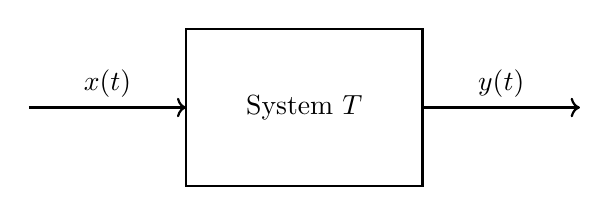
\begin{tikzpicture}[scale=1]
\draw[->,thick] (-3,0) -- (-1,0) node[midway,above] {$x(t)$};
\draw[thick] (-1,-1) rectangle (2,1);
\node at (0.5,0) {System $T$};
\draw[->,thick] (2,0) -- (4,0) node[midway,above] {$y(t)$};
\end{tikzpicture}
\end{center}

The system receives \(x(t)\) and produces \(y(t)\).

%%%%%%%%%%%%%%%%%%%%%%%%%%%%%%%%%%%%%%%%%%%%%%%%%%%%%%%%%%%%%%%%%%%%%%%%%%%%%%%%

\section{Continuous-Time and Discrete-Time Systems}

%%%%%%%%%%%%%%%%%%%%%%%%%%%%%%%%%%%%%%%%%%%%%%%%%%%%%%%%%%%%%%%%%%%%%%%%%%%%%%%%

\subsection{Continuous-Time System}

Input and output are continuous-time signals.

Example:

\[
y(t)=2x(t)+5
\]

%%%%%%%%%%%%%%%%%%%%%%%%%%%%%%%%%%%%%%%%%%%%%%%%%%%%%%%%%%%%%%%%%%%%%%%%%%%%%%%%

\subsection{Discrete-Time System}

Input and output are discrete-time signals.

Example:

\[
y[n]=x[n]+x[n-1]
\]

%%%%%%%%%%%%%%%%%%%%%%%%%%%%%%%%%%%%%%%%%%%%%%%%%%%%%%%%%%%%%%%%%%%%%%%%%%%%%%%%

\section{Memoryless and Dynamic Systems}

%%%%%%%%%%%%%%%%%%%%%%%%%%%%%%%%%%%%%%%%%%%%%%%%%%%%%%%%%%%%%%%%%%%%%%%%%%%%%%%%

\subsection{Memoryless System}

A system is memoryless if the output at time \(t\) depends only on the input at
the same time \(t\).

\[
\boxed{
y(t)=f(x(t))
}
\]

Example:

\[
y(t)=3x(t)
\]

This system is memoryless.

%%%%%%%%%%%%%%%%%%%%%%%%%%%%%%%%%%%%%%%%%%%%%%%%%%%%%%%%%%%%%%%%%%%%%%%%%%%%%%%%

\subsection{Dynamic System}

A system has memory if the output depends on past or future values of the input.

Example:

\[
y(t)=x(t)+x(t-1)
\]

Since \(x(t-1)\) is involved, the system is dynamic.

%%%%%%%%%%%%%%%%%%%%%%%%%%%%%%%%%%%%%%%%%%%%%%%%%%%%%%%%%%%%%%%%%%%%%%%%%%%%%%%%

\section{Linear and Nonlinear Systems}

%%%%%%%%%%%%%%%%%%%%%%%%%%%%%%%%%%%%%%%%%%%%%%%%%%%%%%%%%%%%%%%%%%%%%%%%%%%%%%%%

\subsection{Linearity Conditions}

A system is linear if it satisfies

\begin{enumerate}
\item \textbf{Additivity}
\item \textbf{Homogeneity (scaling)}
\end{enumerate}

%%%%%%%%%%%%%%%%%%%%%%%%%%%%%%%%%%%%%%%%%%%%%%%%%%%%%%%%%%%%%%%%%%%%%%%%%%%%%%%%

\subsection{Additivity}

If

\[
T\{x_1(t)\}=y_1(t)
\]

\[
T\{x_2(t)\}=y_2(t),
\]

then

\[
\boxed{
T\{x_1(t)+x_2(t)\}=y_1(t)+y_2(t)
}
\]

%%%%%%%%%%%%%%%%%%%%%%%%%%%%%%%%%%%%%%%%%%%%%%%%%%%%%%%%%%%%%%%%%%%%%%%%%%%%%%%%

\subsection{Homogeneity}

For any constant \(a\),

\[
\boxed{
T\{ax(t)\}=aT\{x(t)\}
}
\]

%%%%%%%%%%%%%%%%%%%%%%%%%%%%%%%%%%%%%%%%%%%%%%%%%%%%%%%%%%%%%%%%%%%%%%%%%%%%%%%%

\subsection{Superposition}

Combining both conditions,

\[
\boxed{
T\{a_1x_1(t)+a_2x_2(t)\}
=
a_1y_1(t)+a_2y_2(t)
}
\]

This is the superposition principle.

%%%%%%%%%%%%%%%%%%%%%%%%%%%%%%%%%%%%%%%%%%%%%%%%%%%%%%%%%%%%%%%%%%%%%%%%%%%%%%%%

\section{Example: Linear System}

Consider

\[
y(t)=2x(t).
\]

For input \(ax_1(t)+bx_2(t)\),

\[
T\{ax_1+bx_2\}
=
2(ax_1+bx_2)
\]

\[
=2ax_1+2bx_2
\]

\[
=a(2x_1)+b(2x_2)
\]

\[
=aT\{x_1\}+bT\{x_2\}.
\]

Hence,

\[
\boxed{
y(t)=2x(t)\ \text{is linear}
}
\]

%%%%%%%%%%%%%%%%%%%%%%%%%%%%%%%%%%%%%%%%%%%%%%%%%%%%%%%%%%%%%%%%%%%%%%%%%%%%%%%%

\section{Example: Nonlinear System}

Consider

\[
y(t)=x^2(t).
\]

For input \(ax(t)\),

\[
T\{ax(t)\}=(ax(t))^2=a^2x^2(t).
\]

But

\[
aT\{x(t)\}=ax^2(t).
\]

Since

\[
a^2x^2(t)\neq ax^2(t),
\]

the homogeneity condition fails.

Therefore,

\[
\boxed{
y(t)=x^2(t)\ \text{is nonlinear}
}
\]

%%%%%%%%%%%%%%%%%%%%%%%%%%%%%%%%%%%%%%%%%%%%%%%%%%%%%%%%%%%%%%%%%%%%%%%%%%%%%%%%

\section{Time-Invariant Systems}

%%%%%%%%%%%%%%%%%%%%%%%%%%%%%%%%%%%%%%%%%%%%%%%%%%%%%%%%%%%%%%%%%%%%%%%%%%%%%%%%

\subsection{Definition}

A system is time invariant if a delay in the input produces the same delay in
the output.

%%%%%%%%%%%%%%%%%%%%%%%%%%%%%%%%%%%%%%%%%%%%%%%%%%%%%%%%%%%%%%%%%%%%%%%%%%%%%%%%

\subsection{Test Procedure}

Suppose

\[
T\{x(t)\}=y(t).
\]

Delay the input:

\[
x_d(t)=x(t-t_0).
\]

Compute the system output:

\[
T\{x(t-t_0)\}.
\]

Now delay the original output:

\[
y(t-t_0).
\]

If

\[
\boxed{
T\{x(t-t_0)\}=y(t-t_0)
}
\]

the system is time invariant.

%%%%%%%%%%%%%%%%%%%%%%%%%%%%%%%%%%%%%%%%%%%%%%%%%%%%%%%%%%%%%%%%%%%%%%%%%%%%%%%%

\section{Example: Time-Invariant System}

Consider

\[
y(t)=x(t)+x(t-1).
\]

For delayed input,

\[
T\{x(t-t_0)\}
=
x(t-t_0)+x(t-t_0-1).
\]

The delayed output is

\[
y(t-t_0)
=
x(t-t_0)+x(t-t_0-1).
\]

Both are identical.

Hence,

\[
\boxed{
y(t)=x(t)+x(t-1)\ \text{is time invariant}
}
\]

%%%%%%%%%%%%%%%%%%%%%%%%%%%%%%%%%%%%%%%%%%%%%%%%%%%%%%%%%%%%%%%%%%%%%%%%%%%%%%%%

\section{Example: Time-Varying System}

Consider

\[
y(t)=tx(t).
\]

For delayed input,

\[
T\{x(t-t_0)\}=t\,x(t-t_0).
\]

Delayed output:

\[
y(t-t_0)=(t-t_0)x(t-t_0).
\]

Since these are not equal,

\[
\boxed{
y(t)=tx(t)\ \text{is time varying}
}
\]

%%%%%%%%%%%%%%%%%%%%%%%%%%%%%%%%%%%%%%%%%%%%%%%%%%%%%%%%%%%%%%%%%%%%%%%%%%%%%%%%

\section{Quick Identification Table}

\begin{table}[H]
\centering
\caption{Quick classification}
\begin{tabular}{|p{5cm}|p{5cm}|}
\hline
\textbf{System} & \textbf{Classification} \\
\hline
\(y(t)=3x(t)\) & Linear, memoryless, TI \\
\hline
\(y(t)=x^2(t)\) & Nonlinear \\
\hline
\(y(t)=x(t-1)\) & Linear, dynamic, TI \\
\hline
\(y(t)=tx(t)\) & Linear, time varying \\
\hline
\(y(t)=x(t)+5\) & Nonlinear (fails homogeneity) \\
\hline
\end{tabular}
\end{table}

%%%%%%%%%%%%%%%%%%%%%%%%%%%%%%%%%%%%%%%%%%%%%%%%%%%%%%%%%%%%%%%%%%%%%%%%%%%%%%%%

\begin{tcolorbox}[title=Quick Recall,colback=yellow!10]

\[
y(t)=T\{x(t)\}
\]

\[
T\{a_1x_1+a_2x_2\}=a_1T\{x_1\}+a_2T\{x_2\}
\]

\[
T\{x(t-t_0)\}=y(t-t_0)
\]

Memoryless: depends only on \(x(t)\)

Dynamic: depends on \(x(t\pm\tau)\)

\end{tcolorbox}
%%%%%%%%%%%%%%%%%%%%%%%%%%%%%%%%%%%%%%%%%%%%%%%%%%%%%%%%%%%%%%%%%%%%%%%%%%%%%%%%
%%%%%%%%%%%%%%%%%%%%%%%%%%%%%%%%%%%%%%%%%%%%%%%%%%%%%%%%%%%%%%%%%%%%%%%%%%%%%%%%
\section{Causal and Noncausal Systems}

%%%%%%%%%%%%%%%%%%%%%%%%%%%%%%%%%%%%%%%%%%%%%%%%%%%%%%%%%%%%%%%%%%%%%%%%%%%%%%%%

\subsection{Definition of Causality}

A system is \textbf{causal} if the output at time \(t\) depends only on

\begin{itemize}
\item present input values,
\item and past input values.
\end{itemize}

Mathematically, a causal system cannot depend on \(x(t+\tau)\) where
\(\tau>0\).

%%%%%%%%%%%%%%%%%%%%%%%%%%%%%%%%%%%%%%%%%%%%%%%%%%%%%%%%%%%%%%%%%%%%%%%%%%%%%%%%

\subsection{Examples of Causal Systems}

\[
y(t)=x(t)
\]

\[
y(t)=x(t-2)
\]

\[
y(t)=x(t)+x(t-1)
\]

These systems use only present or past values of the input.

%%%%%%%%%%%%%%%%%%%%%%%%%%%%%%%%%%%%%%%%%%%%%%%%%%%%%%%%%%%%%%%%%%%%%%%%%%%%%%%%

\subsection{Example of a Noncausal System}

\[
y(t)=x(t+1)
\]

Here, the output at time \(t\) depends on the future value of the input.

Therefore,

\[
\boxed{
y(t)=x(t+1)\ \text{is noncausal}
}
\]

%%%%%%%%%%%%%%%%%%%%%%%%%%%%%%%%%%%%%%%%%%%%%%%%%%%%%%%%%%%%%%%%%%%%%%%%%%%%%%%%

\section{Causality Test}

For a system described by

\[
y(t)=f(x(t),x(t-1),x(t+1),\ldots),
\]

\begin{itemize}
\item if only \(x(t)\) and \(x(t-\tau)\) appear, the system is causal;
\item if any \(x(t+\tau)\) appears, the system is noncausal.
\end{itemize}

%%%%%%%%%%%%%%%%%%%%%%%%%%%%%%%%%%%%%%%%%%%%%%%%%%%%%%%%%%%%%%%%%%%%%%%%%%%%%%%%

\section{Stability}

%%%%%%%%%%%%%%%%%%%%%%%%%%%%%%%%%%%%%%%%%%%%%%%%%%%%%%%%%%%%%%%%%%%%%%%%%%%%%%%%

\subsection{BIBO Stability}

A system is \textbf{bounded-input bounded-output (BIBO) stable} if every bounded
input produces a bounded output.

If

\[
|x(t)|\le M_x<\infty,
\]

then there must exist a finite constant \(M_y\) such that

\[
|y(t)|\le M_y<\infty.
\]

%%%%%%%%%%%%%%%%%%%%%%%%%%%%%%%%%%%%%%%%%%%%%%%%%%%%%%%%%%%%%%%%%%%%%%%%%%%%%%%%

\section{Example: Stable System}

Consider

\[
y(t)=0.5\,x(t).
\]

If

\[
|x(t)|\le M,
\]

then

\[
|y(t)|=0.5|x(t)|\le 0.5M.
\]

Since \(0.5M\) is finite,

\[
\boxed{
y(t)=0.5x(t)\ \text{is stable}
}
\]

%%%%%%%%%%%%%%%%%%%%%%%%%%%%%%%%%%%%%%%%%%%%%%%%%%%%%%%%%%%%%%%%%%%%%%%%%%%%%%%%

\section{Example: Unstable System}

Consider

\[
y(t)=t\,x(t).
\]

Choose a bounded input

\[
x(t)=1.
\]

Then

\[
y(t)=t.
\]

As \(t\to\infty\),

\[
|y(t)|\to\infty.
\]

Hence,

\[
\boxed{
y(t)=t\,x(t)\ \text{is unstable}
}
\]

%%%%%%%%%%%%%%%%%%%%%%%%%%%%%%%%%%%%%%%%%%%%%%%%%%%%%%%%%%%%%%%%%%%%%%%%%%%%%%%%

\section{Stability of LTI Systems}

For a continuous-time LTI system with impulse response \(h(t)\),

\[
\boxed{
\int_{-\infty}^{\infty}|h(t)|\,dt<\infty
}
\]

is the condition for BIBO stability.

For a discrete-time LTI system,

\[
\boxed{
\sum_{n=-\infty}^{\infty}|h[n]|<\infty
}
\]

%%%%%%%%%%%%%%%%%%%%%%%%%%%%%%%%%%%%%%%%%%%%%%%%%%%%%%%%%%%%%%%%%%%%%%%%%%%%%%%%

\section{Example Using Impulse Response}

Suppose

\[
h(t)=e^{-t}u(t).
\]

Then,

\[
\int_{-\infty}^{\infty}|h(t)|dt
=
\int_0^\infty e^{-t}dt
\]

\[
=
\left[-e^{-t}\right]_0^\infty
=1.
\]

Since the integral is finite,

\[
\boxed{
h(t)=e^{-t}u(t)\ \text{is stable}
}
\]

%%%%%%%%%%%%%%%%%%%%%%%%%%%%%%%%%%%%%%%%%%%%%%%%%%%%%%%%%%%%%%%%%%%%%%%%%%%%%%%%

\section{Invertible Systems}

%%%%%%%%%%%%%%%%%%%%%%%%%%%%%%%%%%%%%%%%%%%%%%%%%%%%%%%%%%%%%%%%%%%%%%%%%%%%%%%%

\subsection{Definition}

A system is \textbf{invertible} if different inputs produce different outputs
and the original input can be uniquely recovered from the output.

%%%%%%%%%%%%%%%%%%%%%%%%%%%%%%%%%%%%%%%%%%%%%%%%%%%%%%%%%%%%%%%%%%%%%%%%%%%%%%%%

\subsection{Example: Invertible}

\[
y(t)=2x(t).
\]

The inverse system is

\[
x(t)=\frac{y(t)}{2}.
\]

Hence,

\[
\boxed{
y(t)=2x(t)\ \text{is invertible}
}
\]

%%%%%%%%%%%%%%%%%%%%%%%%%%%%%%%%%%%%%%%%%%%%%%%%%%%%%%%%%%%%%%%%%%%%%%%%%%%%%%%%

\subsection{Example: Noninvertible}

\[
y(t)=x^2(t).
\]

If

\[
x_1(t)=1,\qquad x_2(t)=-1,
\]

both produce

\[
y(t)=1.
\]

Since the input cannot be uniquely determined,

\[
\boxed{
y(t)=x^2(t)\ \text{is noninvertible}
}
\]

%%%%%%%%%%%%%%%%%%%%%%%%%%%%%%%%%%%%%%%%%%%%%%%%%%%%%%%%%%%%%%%%%%%%%%%%%%%%%%%%

\section{Static and Dynamic Systems}

%%%%%%%%%%%%%%%%%%%%%%%%%%%%%%%%%%%%%%%%%%%%%%%%%%%%%%%%%%%%%%%%%%%%%%%%%%%%%%%%

\subsection{Static (Memoryless)}

\[
y(t)=f(x(t))
\]

Example:

\[
y(t)=5x(t).
\]

%%%%%%%%%%%%%%%%%%%%%%%%%%%%%%%%%%%%%%%%%%%%%%%%%%%%%%%%%%%%%%%%%%%%%%%%%%%%%%%%

\subsection{Dynamic (With Memory)}

\[
y(t)=f(x(t),x(t-\tau),x(t+\tau),\ldots)
\]

Example:

\[
y(t)=x(t)+x(t-1).
\]

%%%%%%%%%%%%%%%%%%%%%%%%%%%%%%%%%%%%%%%%%%%%%%%%%%%%%%%%%%%%%%%%%%%%%%%%%%%%%%%%

\section{Complete Classification Procedure}

Given a system:

\[
y(t)=f(x(t),x(t\pm\tau),t),
\]

use the following sequence:

%%%%%%%%%%%%%%%%%%%%%%%%%%%%%%%%%%%%%%%%%%%%%%%%%%%%%%%%%%%%%%%%%%%%%%%%%%%%%%%%

\subsection{Step 1: Memory}

\begin{itemize}
\item only \(x(t)\) \(\rightarrow\) memoryless,
\item delayed/advanced terms \(\rightarrow\) dynamic.
\end{itemize}

%%%%%%%%%%%%%%%%%%%%%%%%%%%%%%%%%%%%%%%%%%%%%%%%%%%%%%%%%%%%%%%%%%%%%%%%%%%%%%%%

\subsection{Step 2: Linearity}

Check superposition:

\[
T\{a_1x_1+a_2x_2\}
\stackrel{?}{=}
a_1T\{x_1\}+a_2T\{x_2\}.
\]

%%%%%%%%%%%%%%%%%%%%%%%%%%%%%%%%%%%%%%%%%%%%%%%%%%%%%%%%%%%%%%%%%%%%%%%%%%%%%%%%

\subsection{Step 3: Time Invariance}

Check

\[
T\{x(t-t_0)\}
\stackrel{?}{=}
y(t-t_0).
\]

%%%%%%%%%%%%%%%%%%%%%%%%%%%%%%%%%%%%%%%%%%%%%%%%%%%%%%%%%%%%%%%%%%%%%%%%%%%%%%%%

\subsection{Step 4: Causality}

Look for future terms \(x(t+\tau)\).

%%%%%%%%%%%%%%%%%%%%%%%%%%%%%%%%%%%%%%%%%%%%%%%%%%%%%%%%%%%%%%%%%%%%%%%%%%%%%%%%

\subsection{Step 5: Stability}

Apply the BIBO test.

%%%%%%%%%%%%%%%%%%%%%%%%%%%%%%%%%%%%%%%%%%%%%%%%%%%%%%%%%%%%%%%%%%%%%%%%%%%%%%%%

\subsection{Step 6: Invertibility}

Determine whether the input can be uniquely recovered.

%%%%%%%%%%%%%%%%%%%%%%%%%%%%%%%%%%%%%%%%%%%%%%%%%%%%%%%%%%%%%%%%%%%%%%%%%%%%%%%%

\section{Flowchart}

For quick classification of a system, follow this sequence:

\begin{enumerate}
\item Check whether the output depends only on the present input.
\item Check linearity using the superposition principle.
\item Check time invariance.
\item Check causality.
\item Check stability.
\item Check invertibility.
\end{enumerate}

This procedure is sufficient for solving most GATE and university examination problems.
%%%%%%%%%%%%%%%%%%%%%%%%%%%%%%%%%%%%%%%%%%%%%%%%%%%%%%%%%%%%%%%%%%%%%%%%%%%%%%%%

\section{Solved Classification Example}

Classify

\[
y(t)=x(t-1)+3x(t).
\]

%%%%%%%%%%%%%%%%%%%%%%%%%%%%%%%%%%%%%%%%%%%%%%%%%%%%%%%%%%%%%%%%%%%%%%%%%%%%%%%%

\subsection{Memory}

Depends on \(x(t-1)\) \(\Rightarrow\) dynamic.

%%%%%%%%%%%%%%%%%%%%%%%%%%%%%%%%%%%%%%%%%%%%%%%%%%%%%%%%%%%%%%%%%%%%%%%%%%%%%%%%

\subsection{Linearity}

Satisfies superposition \(\Rightarrow\) linear.

%%%%%%%%%%%%%%%%%%%%%%%%%%%%%%%%%%%%%%%%%%%%%%%%%%%%%%%%%%%%%%%%%%%%%%%%%%%%%%%%

\subsection{Time Invariance}

Delay property is preserved \(\Rightarrow\) time invariant.

%%%%%%%%%%%%%%%%%%%%%%%%%%%%%%%%%%%%%%%%%%%%%%%%%%%%%%%%%%%%%%%%%%%%%%%%%%%%%%%%

\subsection{Causality}

Only present and past values appear \(\Rightarrow\) causal.

%%%%%%%%%%%%%%%%%%%%%%%%%%%%%%%%%%%%%%%%%%%%%%%%%%%%%%%%%%%%%%%%%%%%%%%%%%%%%%%%

\subsection{Stability}

Bounded input gives bounded output \(\Rightarrow\) stable.

%%%%%%%%%%%%%%%%%%%%%%%%%%%%%%%%%%%%%%%%%%%%%%%%%%%%%%%%%%%%%%%%%%%%%%%%%%%%%%%%

\subsection{Final Classification}

\[
\boxed{
\text{Linear, Dynamic, Time-Invariant, Causal, Stable}
}
\]

%%%%%%%%%%%%%%%%%%%%%%%%%%%%%%%%%%%%%%%%%%%%%%%%%%%%%%%%%%%%%%%%%%%%%%%%%%%%%%%%

\section{Quick Classification Table}

\begin{table}[H]
\centering
\caption{Common systems and their properties}
\begin{tabular}{|p{5cm}|p{6cm}|}
\hline
\textbf{System} & \textbf{Properties} \\
\hline
\(y(t)=3x(t)\) & Linear, memoryless, TI, causal, stable \\
\hline
\(y(t)=x(t-2)\) & Linear, dynamic, TI, causal, stable \\
\hline
\(y(t)=x(t+2)\) & Linear, dynamic, TI, noncausal, stable \\
\hline
\(y(t)=tx(t)\) & Linear, memoryless, time varying, causal, unstable \\
\hline
\(y(t)=x^2(t)\) & Nonlinear, memoryless, TI, causal \\
\hline
\end{tabular}
\end{table}

%%%%%%%%%%%%%%%%%%%%%%%%%%%%%%%%%%%%%%%%%%%%%%%%%%%%%%%%%%%%%%%%%%%%%%%%%%%%%%%%

\section{Chapter Summary}

In this chapter, we introduced the concept of systems and studied their most
important properties:

\begin{itemize}
\item memoryless and dynamic,
\item linear and nonlinear,
\item time invariant and time varying,
\item causal and noncausal,
\item stable and unstable,
\item invertible and noninvertible.
\end{itemize}

These properties are fundamental for analyzing communication systems, filters,
control systems and digital signal-processing algorithms. In the next chapter,
we will study \textbf{Linear Time-Invariant (LTI) systems} and their impulse
response and convolution properties.

%%%%%%%%%%%%%%%%%%%%%%%%%%%%%%%%%%%%%%%%%%%%%%%%%%%%%%%%%%%%%%%%%%%%%%%%%%%%%%%%

\begin{tcolorbox}[title=One-Minute Revision,colback=blue!5]

\[
T\{a_1x_1+a_2x_2\}=a_1T\{x_1\}+a_2T\{x_2\}
\]

\[
T\{x(t-t_0)\}=y(t-t_0)
\]

Causal: no \(x(t+\tau)\)

Stable: bounded input \(\Rightarrow\) bounded output

Invertible: input can be uniquely recovered

LTI stability:

\[
\int_{-\infty}^{\infty}|h(t)|dt<\infty
\]

\[
\sum_{n=-\infty}^{\infty}|h[n]|<\infty
\]

\end{tcolorbox}
%%%%%%%%%%%%%%%%%%%%%%%%%%%%%%%%%%%%%%%%%%%%%%%%%%%%%%%%%%%%%%%%%%%%%%%%%%%%%%%%

%%%%%%%%%%%%%%%%%%%%%%%%%%%%%%%%%%%%%%%%%%%%%%%%%%%%%%%%%%%%%%%%%%%%%%%%%%%%%%%%
% CHAPTER 3
%%%%%%%%%%%%%%%%%%%%%%%%%%%%%%%%%%%%%%%%%%%%%%%%%%%%%%%%%%%%%%%%%%%%%%%%%%%%%%%%

\chapter{Continuous-Time LTI Systems and Convolution}

\begin{tcolorbox}[colback=blue!5!white,colframe=blue!70!black,title=Learning Objectives]

After studying this chapter, the reader will be able to

\begin{itemize}
\item Define a continuous-time LTI system.
\item Understand impulse response and its significance.
\item Derive the convolution integral.
\item Compute the output of an LTI system using convolution.
\item Understand the graphical interpretation of convolution.
\item Use the properties of convolution in problem solving.
\end{itemize}

\end{tcolorbox}

%%%%%%%%%%%%%%%%%%%%%%%%%%%%%%%%%%%%%%%%%%%%%%%%%%%%%%%%%%%%%%%%%%%%%%%%%%%%%%%%

\section{Introduction}

A \textbf{Linear Time-Invariant (LTI) system} is the most important class of
systems in Signals and Systems because

\begin{itemize}
\item they are mathematically tractable,
\item they model many practical physical systems,
\item and their behavior is completely determined by a single signal called the
impulse response.
\end{itemize}

Examples of systems that can often be modeled as LTI systems include

\begin{itemize}
\item RC circuits,
\item RL circuits,
\item mechanical mass-spring systems,
\item communication channels,
\item and many filters used in signal processing.
\end{itemize}

%%%%%%%%%%%%%%%%%%%%%%%%%%%%%%%%%%%%%%%%%%%%%%%%%%%%%%%%%%%%%%%%%%%%%%%%%%%%%%%%

\section{Definition of an LTI System}

A system is LTI if it satisfies

\begin{enumerate}
\item \textbf{Linearity}
\item \textbf{Time invariance}
\end{enumerate}

%%%%%%%%%%%%%%%%%%%%%%%%%%%%%%%%%%%%%%%%%%%%%%%%%%%%%%%%%%%%%%%%%%%%%%%%%%%%%%%%

\subsection{Linearity}

For inputs \(x_1(t)\) and \(x_2(t)\),

\[
T\{a_1x_1(t)+a_2x_2(t)\}
=
a_1T\{x_1(t)\}+a_2T\{x_2(t)\}.
\]

%%%%%%%%%%%%%%%%%%%%%%%%%%%%%%%%%%%%%%%%%%%%%%%%%%%%%%%%%%%%%%%%%%%%%%%%%%%%%%%%

\subsection{Time Invariance}

If

\[
T\{x(t)\}=y(t),
\]

then

\[
T\{x(t-t_0)\}=y(t-t_0).
\]

%%%%%%%%%%%%%%%%%%%%%%%%%%%%%%%%%%%%%%%%%%%%%%%%%%%%%%%%%%%%%%%%%%%%%%%%%%%%%%%%

\section{Impulse Response}

%%%%%%%%%%%%%%%%%%%%%%%%%%%%%%%%%%%%%%%%%%%%%%%%%%%%%%%%%%%%%%%%%%%%%%%%%%%%%%%%

\subsection{Definition}

The response of an LTI system to a unit impulse input is called the
\textbf{impulse response}.

If

\[
x(t)=\delta(t),
\]

then

\[
\boxed{
y(t)=h(t)
}
\]

where \(h(t)\) is the impulse response.

%%%%%%%%%%%%%%%%%%%%%%%%%%%%%%%%%%%%%%%%%%%%%%%%%%%%%%%%%%%%%%%%%%%%%%%%%%%%%%%%

\subsection{Why is \(h(t)\) Important?}

For an LTI system, knowing \(h(t)\) is sufficient to determine the output for
\emph{any} input signal.

\[
\boxed{
\text{Input }x(t)
\quad \xrightarrow{\text{LTI}}
\quad
\text{Output }y(t)
}
\]

The relationship between \(x(t)\) and \(h(t)\) is called
\textbf{convolution}.

%%%%%%%%%%%%%%%%%%%%%%%%%%%%%%%%%%%%%%%%%%%%%%%%%%%%%%%%%%%%%%%%%%%%%%%%%%%%%%%%

\section{Impulse Decomposition of a Signal}

Any signal can be represented as a continuous sum of shifted impulses:

\[
\boxed{
x(t)=\int_{-\infty}^{\infty}x(\tau)\delta(t-\tau)\,d\tau
}
\]

This is obtained from the sifting property of the delta function.

%%%%%%%%%%%%%%%%%%%%%%%%%%%%%%%%%%%%%%%%%%%%%%%%%%%%%%%%%%%%%%%%%%%%%%%%%%%%%%%%

\section{Response to a Shifted Impulse}

For input

\[
\delta(t-\tau),
\]

the output is

\[
h(t-\tau).
\]

Because of linearity and time invariance,

\[
\boxed{
\delta(t-\tau)\ \longrightarrow\ h(t-\tau)
}
\]

%%%%%%%%%%%%%%%%%%%%%%%%%%%%%%%%%%%%%%%%%%%%%%%%%%%%%%%%%%%%%%%%%%%%%%%%%%%%%%%%

\section{Derivation of the Convolution Integral}

Starting from

\[
x(t)=\int_{-\infty}^{\infty}x(\tau)\delta(t-\tau)\,d\tau,
\]

apply the system operator:

\[
y(t)=T\{x(t)\}.
\]

Using linearity,

\[
y(t)=
\int_{-\infty}^{\infty}
x(\tau)\,T\{\delta(t-\tau)\}\,d\tau.
\]

Since

\[
T\{\delta(t-\tau)\}=h(t-\tau),
\]

we obtain

\[
\boxed{
y(t)=\int_{-\infty}^{\infty}x(\tau)h(t-\tau)\,d\tau
}
\]

This is the \textbf{convolution integral}.

%%%%%%%%%%%%%%%%%%%%%%%%%%%%%%%%%%%%%%%%%%%%%%%%%%%%%%%%%%%%%%%%%%%%%%%%%%%%%%%%

\section{Convolution Notation}

\[
\boxed{
y(t)=x(t)*h(t)
}
\]

where \(*\) denotes convolution.

Thus,

\[
\boxed{
x(t)*h(t)
=
\int_{-\infty}^{\infty}x(\tau)h(t-\tau)\,d\tau
}
\]

%%%%%%%%%%%%%%%%%%%%%%%%%%%%%%%%%%%%%%%%%%%%%%%%%%%%%%%%%%%%%%%%%%%%%%%%%%%%%%%%

\section{Graphical Interpretation}

Convolution can be understood through four steps:

%%%%%%%%%%%%%%%%%%%%%%%%%%%%%%%%%%%%%%%%%%%%%%%%%%%%%%%%%%%%%%%%%%%%%%%%%%%%%%%%

\subsection{Step 1: Flip}

Replace \(h(\tau)\) by

\[
h(-\tau).
\]

%%%%%%%%%%%%%%%%%%%%%%%%%%%%%%%%%%%%%%%%%%%%%%%%%%%%%%%%%%%%%%%%%%%%%%%%%%%%%%%%

\subsection{Step 2: Shift}

Shift by \(t\):

\[
h(t-\tau).
\]

%%%%%%%%%%%%%%%%%%%%%%%%%%%%%%%%%%%%%%%%%%%%%%%%%%%%%%%%%%%%%%%%%%%%%%%%%%%%%%%%

\subsection{Step 3: Multiply}

Multiply

\[
x(\tau)\,h(t-\tau).
\]

%%%%%%%%%%%%%%%%%%%%%%%%%%%%%%%%%%%%%%%%%%%%%%%%%%%%%%%%%%%%%%%%%%%%%%%%%%%%%%%%

\subsection{Step 4: Integrate}

Integrate over all \(\tau\):

\[
y(t)=\int x(\tau)h(t-\tau)\,d\tau.
\]

%%%%%%%%%%%%%%%%%%%%%%%%%%%%%%%%%%%%%%%%%%%%%%%%%%%%%%%%%%%%%%%%%%%%%%%%%%%%%%%%

\section{Convolution of Two Unit Steps}

Let

\[
x(t)=u(t),
\qquad
h(t)=u(t).
\]

Then,

\[
y(t)=\int_{-\infty}^{\infty}u(\tau)u(t-\tau)\,d\tau.
\]

%%%%%%%%%%%%%%%%%%%%%%%%%%%%%%%%%%%%%%%%%%%%%%%%%%%%%%%%%%%%%%%%%%%%%%%%%%%%%%%%

\subsection{Determine Limits}

The integrand is nonzero when

\[
\tau\ge0
\]

and

\[
t-\tau\ge0
\quad\Rightarrow\quad
\tau\le t.
\]

Therefore,

\[
0\le\tau\le t.
\]

%%%%%%%%%%%%%%%%%%%%%%%%%%%%%%%%%%%%%%%%%%%%%%%%%%%%%%%%%%%%%%%%%%%%%%%%%%%%%%%%

\subsection{Evaluate}

\[
y(t)=\int_0^t 1\,d\tau=t.
\]

Hence,

\[
\boxed{
u(t)*u(t)=t\,u(t)
}
\]

This result is extremely important.

%%%%%%%%%%%%%%%%%%%%%%%%%%%%%%%%%%%%%%%%%%%%%%%%%%%%%%%%%%%%%%%%%%%%%%%%%%%%%%%%

\section{Graphical Result}

\begin{center}
\begin{tikzpicture}[scale=0.9]
\draw[->] (-0.5,0) -- (5,0) node[right] {$t$};
\draw[->] (0,-0.5) -- (0,4) node[above] {$y(t)$};

\draw[thick] (-0.5,0) -- (0,0);
\draw[thick] (0,0) -- (4,3.2);
\node[right] at (3,2.6) {$t\,u(t)$};
\end{tikzpicture}
\end{center}

%%%%%%%%%%%%%%%%%%%%%%%%%%%%%%%%%%%%%%%%%%%%%%%%%%%%%%%%%%%%%%%%%%%%%%%%%%%%%%%%

\section{Convolution with an Impulse}

Let

\[
x(t)*\delta(t).
\]

Using the convolution integral,

\[
y(t)=
\int_{-\infty}^{\infty}
x(\tau)\delta(t-\tau)\,d\tau.
\]

By the sifting property,

\[
\boxed{
x(t)*\delta(t)=x(t)
}
\]

Thus, the impulse acts as the identity element for convolution.

%%%%%%%%%%%%%%%%%%%%%%%%%%%%%%%%%%%%%%%%%%%%%%%%%%%%%%%%%%%%%%%%%%%%%%%%%%%%%%%%

\section{Important Convolution Pairs}

\begin{table}[H]
\centering
\caption{Common convolution results}
\begin{tabular}{|p{5cm}|p{5cm}|}
\hline
\textbf{Signals} & \textbf{Result} \\
\hline
\(x(t)*\delta(t)\) & \(x(t)\) \\
\hline
\(u(t)*u(t)\) & \(t\,u(t)\) \\
\hline
\(u(t)*t\,u(t)\) & \(\dfrac{t^2}{2}u(t)\) \\
\hline
\(e^{-at}u(t)*u(t)\) & \(\dfrac{1-e^{-at}}{a}u(t)\) \\
\hline
\end{tabular}
\end{table}

%%%%%%%%%%%%%%%%%%%%%%%%%%%%%%%%%%%%%%%%%%%%%%%%%%%%%%%%%%%%%%%%%%%%%%%%%%%%%%%%

\section{Properties of Convolution}

%%%%%%%%%%%%%%%%%%%%%%%%%%%%%%%%%%%%%%%%%%%%%%%%%%%%%%%%%%%%%%%%%%%%%%%%%%%%%%%%

\subsection{Commutative}

\[
\boxed{
x(t)*h(t)=h(t)*x(t)
}
\]

%%%%%%%%%%%%%%%%%%%%%%%%%%%%%%%%%%%%%%%%%%%%%%%%%%%%%%%%%%%%%%%%%%%%%%%%%%%%%%%%

\subsection{Associative}

\[
\boxed{
[x_1(t)*x_2(t)]*x_3(t)
=
x_1(t)*[x_2(t)*x_3(t)]
}
\]

%%%%%%%%%%%%%%%%%%%%%%%%%%%%%%%%%%%%%%%%%%%%%%%%%%%%%%%%%%%%%%%%%%%%%%%%%%%%%%%%

\subsection{Distributive}

\[
\boxed{
x(t)*[h_1(t)+h_2(t)]
=
x(t)*h_1(t)+x(t)*h_2(t)
}
\]

These properties greatly simplify convolution calculations.

%%%%%%%%%%%%%%%%%%%%%%%%%%%%%%%%%%%%%%%%%%%%%%%%%%%%%%%%%%%%%%%%%%%%%%%%%%%%%%%%

\section{Worked Example 3.1}

Find

\[
y(t)=u(t)*u(t).
\]

\textbf{Solution}

\[
y(t)=\int_{-\infty}^{\infty}u(\tau)u(t-\tau)\,d\tau
\]

The valid region is

\[
0\le\tau\le t.
\]

Therefore,

\[
y(t)=\int_0^t 1\,d\tau=t.
\]

Hence,

\[
\boxed{
y(t)=t\,u(t)
}
\]

%%%%%%%%%%%%%%%%%%%%%%%%%%%%%%%%%%%%%%%%%%%%%%%%%%%%%%%%%%%%%%%%%%%%%%%%%%%%%%%%

\begin{tcolorbox}[title=Quick Recall,colback=yellow!10]

\[
y(t)=x(t)*h(t)
\]

\[
y(t)=\int_{-\infty}^{\infty}x(\tau)h(t-\tau)\,d\tau
\]

\[
u(t)*u(t)=t\,u(t)
\]

\[
x(t)*\delta(t)=x(t)
\]

Flip \(\rightarrow\) Shift \(\rightarrow\) Multiply \(\rightarrow\) Integrate

\end{tcolorbox}
%%%%%%%%%%%%%%%%%%%%%%%%%%%%%%%%%%%%%%%%%%%%%%%%%%%%%%%%%%%%%%%%%%%%%%%%%%%%%%%%
%%%%%%%%%%%%%%%%%%%%%%%%%%%%%%%%%%%%%%%%%%%%%%%%%%%%%%%%%%%%%%%%%%%%%%%%%%%%%%%%
\section{Graphical Convolution in Detail}

Consider

\[
x(t)=u(t),
\qquad
h(t)=u(t)-u(t-1).
\]

The impulse response is a rectangular pulse of width 1.

%%%%%%%%%%%%%%%%%%%%%%%%%%%%%%%%%%%%%%%%%%%%%%%%%%%%%%%%%%%%%%%%%%%%%%%%%%%%%%%%

\subsection{Step 1: Flip}

\[
h(-\tau)=u(-\tau)-u(-\tau-1).
\]

%%%%%%%%%%%%%%%%%%%%%%%%%%%%%%%%%%%%%%%%%%%%%%%%%%%%%%%%%%%%%%%%%%%%%%%%%%%%%%%%

\subsection{Step 2: Shift}

\[
h(t-\tau)=u(t-\tau)-u(t-\tau-1).
\]

%%%%%%%%%%%%%%%%%%%%%%%%%%%%%%%%%%%%%%%%%%%%%%%%%%%%%%%%%%%%%%%%%%%%%%%%%%%%%%%%

\subsection{Step 3: Overlap Region}

The overlap exists when

\[
\tau\ge0
\]

and

\[
t-1\le\tau\le t.
\]

Hence,

\[
\max(0,t-1)\le\tau\le t.
\]

%%%%%%%%%%%%%%%%%%%%%%%%%%%%%%%%%%%%%%%%%%%%%%%%%%%%%%%%%%%%%%%%%%%%%%%%%%%%%%%%

\subsection{Step 4: Integrate}

For \(0<t<1\),

\[
y(t)=\int_0^t 1\,d\tau=t.
\]

For \(t\ge1\),

\[
y(t)=\int_{t-1}^{t}1\,d\tau=1.
\]

Therefore,

\[
\boxed{
y(t)=
\begin{cases}
0, & t<0\\
t, & 0\le t<1\\
1, & t\ge1
\end{cases}
}
\]

%%%%%%%%%%%%%%%%%%%%%%%%%%%%%%%%%%%%%%%%%%%%%%%%%%%%%%%%%%%%%%%%%%%%%%%%%%%%%%%%

\section{Convolution of Rectangular Pulses}

Let

\[
x(t)=u(t)-u(t-T),
\]

\[
h(t)=u(t)-u(t-T).
\]

Both are pulses of width \(T\).

The result is a triangular waveform:

\[
\boxed{
y(t)=
\begin{cases}
0, & t<0\\
t, & 0\le t<T\\
2T-t, & T\le t<2T\\
0, & t\ge2T
\end{cases}
}
\]

%%%%%%%%%%%%%%%%%%%%%%%%%%%%%%%%%%%%%%%%%%%%%%%%%%%%%%%%%%%%%%%%%%%%%%%%%%%%%%%%

\subsection{Graph}

\begin{center}
\begin{tikzpicture}[scale=0.9]
\draw[->] (-0.5,0) -- (5.5,0) node[right] {$t$};
\draw[->] (0,-0.5) -- (0,3) node[above] {$y(t)$};

\draw[thick] (0,0) -- (2,2) -- (4,0);

\node[below] at (2,0) {$T$};
\node[below] at (4,0) {$2T$};
\end{tikzpicture}
\end{center}

This result is frequently asked in GATE.

%%%%%%%%%%%%%%%%%%%%%%%%%%%%%%%%%%%%%%%%%%%%%%%%%%%%%%%%%%%%%%%%%%%%%%%%%%%%%%%%

\section{Convolution with an Exponential}

Let

\[
x(t)=u(t),
\qquad
h(t)=e^{-at}u(t),
\qquad a>0.
\]

%%%%%%%%%%%%%%%%%%%%%%%%%%%%%%%%%%%%%%%%%%%%%%%%%%%%%%%%%%%%%%%%%%%%%%%%%%%%%%%%

\subsection{Convolution Integral}

\[
y(t)=\int_{-\infty}^{\infty}
u(\tau)e^{-a(t-\tau)}u(t-\tau)\,d\tau.
\]

The valid region is

\[
0\le\tau\le t.
\]

Hence,

\[
y(t)=\int_0^t e^{-a(t-\tau)}\,d\tau.
\]

%%%%%%%%%%%%%%%%%%%%%%%%%%%%%%%%%%%%%%%%%%%%%%%%%%%%%%%%%%%%%%%%%%%%%%%%%%%%%%%%

\subsection{Evaluation}

\[
y(t)=e^{-at}\int_0^t e^{a\tau}\,d\tau
\]

\[
=e^{-at}\left[\frac{e^{a\tau}}{a}\right]_0^t
\]

\[
=\frac{1-e^{-at}}{a}.
\]

Therefore,

\[
\boxed{
u(t)*e^{-at}u(t)
=
\frac{1-e^{-at}}{a}u(t)
}
\]

%%%%%%%%%%%%%%%%%%%%%%%%%%%%%%%%%%%%%%%%%%%%%%%%%%%%%%%%%%%%%%%%%%%%%%%%%%%%%%%%

\section{Output of an LTI System}

For any input,

\[
\boxed{
y(t)=x(t)*h(t)
}
\]

Thus, the entire behavior of an LTI system is contained in \(h(t)\).

%%%%%%%%%%%%%%%%%%%%%%%%%%%%%%%%%%%%%%%%%%%%%%%%%%%%%%%%%%%%%%%%%%%%%%%%%%%%%%%%

\section{Causality of CT-LTI Systems}

A continuous-time LTI system is causal if and only if

\[
\boxed{
h(t)=0,\qquad t<0
}
\]

%%%%%%%%%%%%%%%%%%%%%%%%%%%%%%%%%%%%%%%%%%%%%%%%%%%%%%%%%%%%%%%%%%%%%%%%%%%%%%%%

\subsection{Example}

\[
h(t)=e^{-t}u(t)
\]

Since \(u(t)=0\) for \(t<0\),

\[
\boxed{
\text{The system is causal}
}
\]

%%%%%%%%%%%%%%%%%%%%%%%%%%%%%%%%%%%%%%%%%%%%%%%%%%%%%%%%%%%%%%%%%%%%%%%%%%%%%%%%

\section{Stability of CT-LTI Systems}

A CT-LTI system is BIBO stable if

\[
\boxed{
\int_{-\infty}^{\infty}|h(t)|\,dt<\infty
}
\]

%%%%%%%%%%%%%%%%%%%%%%%%%%%%%%%%%%%%%%%%%%%%%%%%%%%%%%%%%%%%%%%%%%%%%%%%%%%%%%%%

\subsection{Example}

\[
h(t)=e^{-t}u(t)
\]

\[
\int_0^\infty e^{-t}dt=1<\infty
\]

Hence,

\[
\boxed{
\text{The system is stable}
}
\]

%%%%%%%%%%%%%%%%%%%%%%%%%%%%%%%%%%%%%%%%%%%%%%%%%%%%%%%%%%%%%%%%%%%%%%%%%%%%%%%%

\section{Impulse Response and Differential Equations}

Many physical systems are described by differential equations.

%%%%%%%%%%%%%%%%%%%%%%%%%%%%%%%%%%%%%%%%%%%%%%%%%%%%%%%%%%%%%%%%%%%%%%%%%%%%%%%%

\subsection{First-Order System}

\[
\boxed{
\frac{dy(t)}{dt}+ay(t)=x(t)
}
\]

To find \(h(t)\), apply

\[
x(t)=\delta(t).
\]

Then,

\[
\frac{dh(t)}{dt}+ah(t)=\delta(t).
\]

The solution is

\[
\boxed{
h(t)=e^{-at}u(t)
}
\]

This is the impulse response of a first-order stable system.

%%%%%%%%%%%%%%%%%%%%%%%%%%%%%%%%%%%%%%%%%%%%%%%%%%%%%%%%%%%%%%%%%%%%%%%%%%%%%%%%

\section{RC Circuit Example}

Consider a series RC circuit with output across the capacitor.

The governing equation is

\[
RC\frac{dy(t)}{dt}+y(t)=x(t).
\]

Comparing with the standard form,

\[
a=\frac{1}{RC}.
\]

Therefore,

\[
\boxed{
h(t)=\frac{1}{RC}e^{-t/(RC)}u(t)
}
\]

%%%%%%%%%%%%%%%%%%%%%%%%%%%%%%%%%%%%%%%%%%%%%%%%%%%%%%%%%%%%%%%%%%%%%%%%%%%%%%%%

\section{Step Response}

The step response is the output for

\[
x(t)=u(t).
\]

Using convolution,

\[
s(t)=u(t)*h(t).
\]

For the RC circuit,

\[
s(t)=
\int_0^t
\frac{1}{RC}e^{-(t-\tau)/(RC)}\,d\tau.
\]

Evaluating,

\[
\boxed{
s(t)=\left(1-e^{-t/(RC)}\right)u(t)
}
\]

This is the familiar charging equation of a capacitor.

%%%%%%%%%%%%%%%%%%%%%%%%%%%%%%%%%%%%%%%%%%%%%%%%%%%%%%%%%%%%%%%%%%%%%%%%%%%%%%%%

\section{Convolution Summary}

\begin{table}[H]
\centering
\caption{Important convolution results}
\begin{tabular}{|p{6cm}|p{5cm}|}
\hline
\textbf{Convolution} & \textbf{Result} \\
\hline
\(x(t)*\delta(t)\) & \(x(t)\) \\
\hline
\(u(t)*u(t)\) & \(t\,u(t)\) \\
\hline
\(u(t)*t\,u(t)\) & \(\dfrac{t^2}{2}u(t)\) \\
\hline
\(u(t)*e^{-at}u(t)\) & \(\dfrac{1-e^{-at}}{a}u(t)\) \\
\hline
Rectangular pulse * rectangular pulse & Triangular pulse \\
\hline
\end{tabular}
\end{table}

%%%%%%%%%%%%%%%%%%%%%%%%%%%%%%%%%%%%%%%%%%%%%%%%%%%%%%%%%%%%%%%%%%%%%%%%%%%%%%%%

\section{Problem-Solving Strategy}

%%%%%%%%%%%%%%%%%%%%%%%%%%%%%%%%%%%%%%%%%%%%%%%%%%%%%%%%%%%%%%%%%%%%%%%%%%%%%%%%

\subsection{Step 1}

Identify \(x(t)\) and \(h(t)\).

%%%%%%%%%%%%%%%%%%%%%%%%%%%%%%%%%%%%%%%%%%%%%%%%%%%%%%%%%%%%%%%%%%%%%%%%%%%%%%%%

\subsection{Step 2}

Write

\[
y(t)=\int x(\tau)h(t-\tau)\,d\tau.
\]

%%%%%%%%%%%%%%%%%%%%%%%%%%%%%%%%%%%%%%%%%%%%%%%%%%%%%%%%%%%%%%%%%%%%%%%%%%%%%%%%

\subsection{Step 3}

Determine the overlap region.

%%%%%%%%%%%%%%%%%%%%%%%%%%%%%%%%%%%%%%%%%%%%%%%%%%%%%%%%%%%%%%%%%%%%%%%%%%%%%%%%

\subsection{Step 4}

Set the correct limits of integration.

%%%%%%%%%%%%%%%%%%%%%%%%%%%%%%%%%%%%%%%%%%%%%%%%%%%%%%%%%%%%%%%%%%%%%%%%%%%%%%%%

\subsection{Step 5}

Evaluate the integral.

%%%%%%%%%%%%%%%%%%%%%%%%%%%%%%%%%%%%%%%%%%%%%%%%%%%%%%%%%%%%%%%%%%%%%%%%%%%%%%%%

\subsection{Step 6}

Express the answer using unit-step functions if required.

%%%%%%%%%%%%%%%%%%%%%%%%%%%%%%%%%%%%%%%%%%%%%%%%%%%%%%%%%%%%%%%%%%%%%%%%%%%%%%%%

\section{Common GATE Mistakes}

\begin{enumerate}
\item Forgetting to flip \(h(\tau)\) before shifting.
\item Using incorrect overlap limits.
\item Forgetting the unit-step multiplier.
\item Confusing convolution with ordinary multiplication.
\item Assuming convolution is not commutative.
\item Ignoring the causality condition \(h(t)=0\) for \(t<0\).
\item Forgetting the absolute value in the stability integral.
\end{enumerate}

%%%%%%%%%%%%%%%%%%%%%%%%%%%%%%%%%%%%%%%%%%%%%%%%%%%%%%%%%%%%%%%%%%%%%%%%%%%%%%%%

\section{Chapter Summary}

In this chapter, we studied continuous-time LTI systems and showed that the
output of an LTI system is obtained by convolving the input with the impulse
response.

We derived the convolution integral from the impulse decomposition of a signal
and learned the graphical interpretation of convolution through the
flip-shift-multiply-integrate procedure.

We also studied

\begin{itemize}
\item convolution of step signals,
\item convolution of rectangular pulses,
\item convolution with exponential signals,
\item causality and stability conditions,
\item and impulse responses obtained from differential equations.
\end{itemize}

These concepts form the foundation for Fourier analysis and frequency-domain
representation of systems.

%%%%%%%%%%%%%%%%%%%%%%%%%%%%%%%%%%%%%%%%%%%%%%%%%%%%%%%%%%%%%%%%%%%%%%%%%%%%%%%%

\begin{tcolorbox}[title=One-Minute Revision,colback=blue!5]

\[
y(t)=x(t)*h(t)
\]

\[
y(t)=\int_{-\infty}^{\infty}x(\tau)h(t-\tau)\,d\tau
\]

\[
u(t)*u(t)=t\,u(t)
\]

\[
u(t)*e^{-at}u(t)=\frac{1-e^{-at}}{a}u(t)
\]

Causal:

\[
h(t)=0,\quad t<0
\]

Stable:

\[
\int_{-\infty}^{\infty}|h(t)|dt<\infty
\]

RC impulse response:

\[
h(t)=\frac{1}{RC}e^{-t/(RC)}u(t)
\]

RC step response:

\[
s(t)=\left(1-e^{-t/(RC)}\right)u(t)
\]

\end{tcolorbox}
%%%%%%%%%%%%%%%%%%%%%%%%%%%%%%%%%%%%%%%%%%%%%%%%%%%%%%%%%%%%%%%%%%%%%%%%%%%%%%%%
%%%%%%%%%%%%%%%%%%%%%%%%%%%%%%%%%%%%%%%%%%%%%%%%%%%%%%%%%%%%%%%%%%%%%%%%%%%%%%%%
% CHAPTER 4
%%%%%%%%%%%%%%%%%%%%%%%%%%%%%%%%%%%%%%%%%%%%%%%%%%%%%%%%%%%%%%%%%%%%%%%%%%%%%%%%

\chapter{Fourier Series}

\begin{tcolorbox}[colback=blue!5!white,colframe=blue!70!black,title=Learning Objectives]

After studying this chapter, the reader will be able to

\begin{itemize}
\item Understand the idea of representing periodic signals as sums of sinusoids.
\item Write the trigonometric Fourier series representation.
\item Derive the Fourier coefficients.
\item Use orthogonality of sine and cosine functions.
\item Determine coefficients for even and odd signals.
\item Find the Fourier series of common waveforms.
\end{itemize}

\end{tcolorbox}

%%%%%%%%%%%%%%%%%%%%%%%%%%%%%%%%%%%%%%%%%%%%%%%%%%%%%%%%%%%%%%%%%%%%%%%%%%%%%%%%

\section{Introduction}

Any periodic signal can be represented as a sum of sinusoidal signals of
different frequencies, amplitudes and phases.

This representation is called the \textbf{Fourier Series}.

The fundamental idea is

\[
\boxed{
\text{Periodic signal}
=
\text{DC component}
+
\text{Harmonics}
}
\]

where the harmonics are sinusoidal components whose frequencies are integer
multiples of the fundamental frequency.

Fourier Series forms the foundation of

\begin{itemize}
\item communication systems,
\item modulation,
\item spectrum analysis,
\item filter design,
\item and digital signal processing.
\end{itemize}

%%%%%%%%%%%%%%%%%%%%%%%%%%%%%%%%%%%%%%%%%%%%%%%%%%%%%%%%%%%%%%%%%%%%%%%%%%%%%%%%

\section{Periodic Signal}

A signal is periodic if

\[
\boxed{
x(t)=x(t+T)
}
\]

where \(T\) is the fundamental period.

The fundamental frequency is

\[
\boxed{
f_0=\frac{1}{T}
}
\]

and the fundamental angular frequency is

\[
\boxed{
\omega_0=\frac{2\pi}{T}
}
\]

%%%%%%%%%%%%%%%%%%%%%%%%%%%%%%%%%%%%%%%%%%%%%%%%%%%%%%%%%%%%%%%%%%%%%%%%%%%%%%%%

\section{Harmonics}

The frequencies present in a Fourier series are

\[
f_0,\ 2f_0,\ 3f_0,\ldots,nf_0.
\]

The \(n\)-th harmonic has angular frequency

\[
\boxed{
n\omega_0
}
\]

%%%%%%%%%%%%%%%%%%%%%%%%%%%%%%%%%%%%%%%%%%%%%%%%%%%%%%%%%%%%%%%%%%%%%%%%%%%%%%%%

\section{Trigonometric Fourier Series}

A periodic signal \(x(t)\) with period \(T\) can be written as

\[
\boxed{
x(t)=
\frac{a_0}{2}
+
\sum_{n=1}^{\infty}
\left[
a_n\cos(n\omega_0 t)
+
b_n\sin(n\omega_0 t)
\right]
}
\]

where

\begin{itemize}
\item \(a_0\): DC coefficient,
\item \(a_n\): cosine coefficients,
\item \(b_n\): sine coefficients.
\end{itemize}

%%%%%%%%%%%%%%%%%%%%%%%%%%%%%%%%%%%%%%%%%%%%%%%%%%%%%%%%%%%%%%%%%%%%%%%%%%%%%%%%

\section{Orthogonality of Trigonometric Functions}

%%%%%%%%%%%%%%%%%%%%%%%%%%%%%%%%%%%%%%%%%%%%%%%%%%%%%%%%%%%%%%%%%%%%%%%%%%%%%%%%

\subsection{Cosine Functions}

\[
\int_0^T
\cos(m\omega_0 t)\cos(n\omega_0 t)\,dt
=
\begin{cases}
0, & m\neq n\\[4pt]
\dfrac{T}{2}, & m=n
\end{cases}
\]

%%%%%%%%%%%%%%%%%%%%%%%%%%%%%%%%%%%%%%%%%%%%%%%%%%%%%%%%%%%%%%%%%%%%%%%%%%%%%%%%

\subsection{Sine Functions}

\[
\int_0^T
\sin(m\omega_0 t)\sin(n\omega_0 t)\,dt
=
\begin{cases}
0, & m\neq n\\[4pt]
\dfrac{T}{2}, & m=n
\end{cases}
\]

%%%%%%%%%%%%%%%%%%%%%%%%%%%%%%%%%%%%%%%%%%%%%%%%%%%%%%%%%%%%%%%%%%%%%%%%%%%%%%%%

\subsection{Sine and Cosine}

\[
\boxed{
\int_0^T
\sin(m\omega_0 t)\cos(n\omega_0 t)\,dt=0
}
\]

These orthogonality relations allow us to extract individual Fourier
coefficients.

%%%%%%%%%%%%%%%%%%%%%%%%%%%%%%%%%%%%%%%%%%%%%%%%%%%%%%%%%%%%%%%%%%%%%%%%%%%%%%%%

\section{Derivation of \(a_0\)}

Multiply the Fourier series by 1 and integrate over one period:

\[
\int_0^T x(t)\,dt
=
\int_0^T
\left[
\frac{a_0}{2}
+\sum_{n=1}^{\infty}(\cdots)
\right]dt
\]

All sine and cosine integrals become zero over one complete period, leaving

\[
\int_0^T x(t)\,dt
=
\frac{a_0}{2}T
\]

Hence,

\[
\boxed{
a_0=\frac{2}{T}\int_0^T x(t)\,dt
}
\]

%%%%%%%%%%%%%%%%%%%%%%%%%%%%%%%%%%%%%%%%%%%%%%%%%%%%%%%%%%%%%%%%%%%%%%%%%%%%%%%%

\section{Derivation of \(a_n\)}

Multiply the Fourier series by \(\cos(m\omega_0 t)\) and integrate:

\[
\int_0^T x(t)\cos(m\omega_0 t)\,dt
=
\frac{a_mT}{2}
\]

Therefore,

\[
\boxed{
a_n=
\frac{2}{T}
\int_0^T
x(t)\cos(n\omega_0 t)\,dt
}
\]

%%%%%%%%%%%%%%%%%%%%%%%%%%%%%%%%%%%%%%%%%%%%%%%%%%%%%%%%%%%%%%%%%%%%%%%%%%%%%%%%

\section{Derivation of \(b_n\)}

Multiply the Fourier series by \(\sin(m\omega_0 t)\) and integrate:

\[
\int_0^T x(t)\sin(m\omega_0 t)\,dt
=
\frac{b_mT}{2}
\]

Hence,

\[
\boxed{
b_n=
\frac{2}{T}
\int_0^T
x(t)\sin(n\omega_0 t)\,dt
}
\]

%%%%%%%%%%%%%%%%%%%%%%%%%%%%%%%%%%%%%%%%%%%%%%%%%%%%%%%%%%%%%%%%%%%%%%%%%%%%%%%%

\section{Summary of Fourier Coefficients}

\begin{tcolorbox}[title=Coefficient Formulas,colback=yellow!10]

\[
a_0=
\frac{2}{T}\int_0^T x(t)\,dt
\]

\[
a_n=
\frac{2}{T}
\int_0^T x(t)\cos(n\omega_0 t)\,dt
\]

\[
b_n=
\frac{2}{T}
\int_0^T x(t)\sin(n\omega_0 t)\,dt
\]

\end{tcolorbox}

%%%%%%%%%%%%%%%%%%%%%%%%%%%%%%%%%%%%%%%%%%%%%%%%%%%%%%%%%%%%%%%%%%%%%%%%%%%%%%%%

\section{Even and Odd Signals}

%%%%%%%%%%%%%%%%%%%%%%%%%%%%%%%%%%%%%%%%%%%%%%%%%%%%%%%%%%%%%%%%%%%%%%%%%%%%%%%%

\subsection{Even Signal}

If

\[
x(t)=x(-t),
\]

then

\[
\boxed{
b_n=0
}
\]

Only cosine terms remain:

\[
x(t)=
\frac{a_0}{2}
+
\sum_{n=1}^{\infty}
a_n\cos(n\omega_0 t)
\]

The coefficients can be computed as

\[
\boxed{
a_n=
\frac{4}{T}
\int_0^{T/2}
x(t)\cos(n\omega_0 t)\,dt
}
\]

%%%%%%%%%%%%%%%%%%%%%%%%%%%%%%%%%%%%%%%%%%%%%%%%%%%%%%%%%%%%%%%%%%%%%%%%%%%%%%%%

\section{Odd Signal}

If

\[
x(t)=-x(-t),
\]

then

\[
\boxed{
a_0=0,\qquad a_n=0
}
\]

Only sine terms remain:

\[
x(t)=
\sum_{n=1}^{\infty}
b_n\sin(n\omega_0 t)
\]

and

\[
\boxed{
b_n=
\frac{4}{T}
\int_0^{T/2}
x(t)\sin(n\omega_0 t)\,dt
}
\]

%%%%%%%%%%%%%%%%%%%%%%%%%%%%%%%%%%%%%%%%%%%%%%%%%%%%%%%%%%%%%%%%%%%%%%%%%%%%%%%%

\section{Half-Wave Symmetry}

A signal has half-wave symmetry if

\[
\boxed{
x\left(t+\frac{T}{2}\right)=-x(t)
}
\]

For such signals,

\[
\boxed{
a_0=0
}
\]

and all even harmonics vanish:

\[
\boxed{
a_{2k}=0,\qquad b_{2k}=0
}
\]

Only odd harmonics are present.

%%%%%%%%%%%%%%%%%%%%%%%%%%%%%%%%%%%%%%%%%%%%%%%%%%%%%%%%%%%%%%%%%%%%%%%%%%%%%%%%

\section{Example: Pure Cosine}

Let

\[
x(t)=A\cos(\omega_0 t).
\]

Comparing with the Fourier series,

\[
a_1=A,
\qquad
a_n=0\ (n\neq1),
\qquad
b_n=0,
\qquad
a_0=0.
\]

Thus, a single sinusoid contains only one harmonic component.

%%%%%%%%%%%%%%%%%%%%%%%%%%%%%%%%%%%%%%%%%%%%%%%%%%%%%%%%%%%%%%%%%%%%%%%%%%%%%%%%

\section{Example: DC Signal}

Let

\[
x(t)=A.
\]

Then

\[
a_0=
\frac{2}{T}\int_0^T A\,dt
=
2A.
\]

Therefore,

\[
\frac{a_0}{2}=A
\]

and all other coefficients are zero.

%%%%%%%%%%%%%%%%%%%%%%%%%%%%%%%%%%%%%%%%%%%%%%%%%%%%%%%%%%%%%%%%%%%%%%%%%%%%%%%%

\section{Graphical Interpretation}

The Fourier series decomposes a periodic waveform into

\begin{itemize}
\item a constant (DC) component,
\item a fundamental sinusoid,
\item and higher-order harmonics.
\end{itemize}

\begin{center}
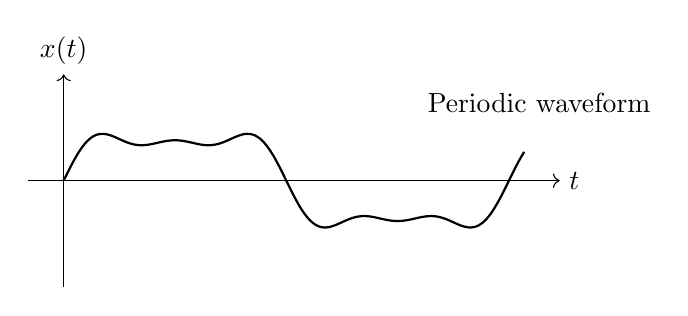
\begin{tikzpicture}[scale=0.9]
\draw[->] (-0.5,0) -- (7,0) node[right] {$t$};
\draw[->] (0,-1.5) -- (0,1.5) node[above] {$x(t)$};

\draw[thick,smooth,samples=100,domain=0:6.5]
plot(\x,{0.7*sin(deg(\x))+0.25*sin(deg(3*\x))+0.12*sin(deg(5*\x))});

\node[right] at (5,1.1) {Periodic waveform};
\end{tikzpicture}
\end{center}

This waveform can be viewed as the sum of the fundamental, third harmonic and
fifth harmonic.

%%%%%%%%%%%%%%%%%%%%%%%%%%%%%%%%%%%%%%%%%%%%%%%%%%%%%%%%%%%%%%%%%%%%%%%%%%%%%%%%

\section{Why Fourier Series Works}

Sinusoids form an orthogonal basis over one period. Just as any vector can be
expressed as a combination of orthogonal unit vectors, any periodic signal can
be expressed as a combination of orthogonal sine and cosine functions.

%%%%%%%%%%%%%%%%%%%%%%%%%%%%%%%%%%%%%%%%%%%%%%%%%%%%%%%%%%%%%%%%%%%%%%%%%%%%%%%%

\begin{tcolorbox}[title=Quick Recall,colback=blue!5]

\[
\omega_0=\frac{2\pi}{T}
\]

\[
x(t)=
\frac{a_0}{2}
+\sum_{n=1}^{\infty}
\left[
a_n\cos(n\omega_0 t)+b_n\sin(n\omega_0 t)
\right]
\]

\[
a_0=
\frac{2}{T}\int_0^T x(t)\,dt
\]

\[
a_n=
\frac{2}{T}\int_0^T x(t)\cos(n\omega_0 t)\,dt
\]

\[
b_n=
\frac{2}{T}\int_0^T x(t)\sin(n\omega_0 t)\,dt
\]

Even signal \(\Rightarrow b_n=0\)

Odd signal \(\Rightarrow a_0=a_n=0\)

Half-wave symmetry \(\Rightarrow\) only odd harmonics

\end{tcolorbox}
%%%%%%%%%%%%%%%%%%%%%%%%%%%%%%%%%%%%%%%%%%%%%%%%%%%%%%%%%%%%%%%%%%%%%%%%%%%%%%%%
%%%%%%%%%%%%%%%%%%%%%%%%%%%%%%%%%%%%%%%%%%%%%%%%%%%%%%%%%%%%%%%%%%%%%%%%%%%%%%%%
\section{Exponential Fourier Series}

%%%%%%%%%%%%%%%%%%%%%%%%%%%%%%%%%%%%%%%%%%%%%%%%%%%%%%%%%%%%%%%%%%%%%%%%%%%%%%%%

\subsection{Euler's Formula}

Using

\[
e^{j\theta}=\cos\theta+j\sin\theta,
\]

the trigonometric Fourier series can be written in a compact exponential form.

%%%%%%%%%%%%%%%%%%%%%%%%%%%%%%%%%%%%%%%%%%%%%%%%%%%%%%%%%%%%%%%%%%%%%%%%%%%%%%%%

\subsection{Exponential Form}

\[
\boxed{
x(t)=\sum_{n=-\infty}^{\infty}C_n e^{jn\omega_0 t}
}
\]

where \(C_n\) are the complex Fourier coefficients.

%%%%%%%%%%%%%%%%%%%%%%%%%%%%%%%%%%%%%%%%%%%%%%%%%%%%%%%%%%%%%%%%%%%%%%%%%%%%%%%%

\section{Derivation of \(C_n\)}

Multiply both sides by \(e^{-jm\omega_0 t}\) and integrate over one period:

\[
\int_0^T x(t)e^{-jm\omega_0 t}dt
=
\sum_{n=-\infty}^{\infty}
C_n
\int_0^T
e^{j(n-m)\omega_0 t}dt
\]

Using orthogonality,

\[
\int_0^T e^{j(n-m)\omega_0 t}dt=
\begin{cases}
T, & n=m\\
0, & n\neq m
\end{cases}
\]

Therefore,

\[
\boxed{
C_n=
\frac{1}{T}
\int_0^T
x(t)e^{-jn\omega_0 t}dt
}
\]

%%%%%%%%%%%%%%%%%%%%%%%%%%%%%%%%%%%%%%%%%%%%%%%%%%%%%%%%%%%%%%%%%%%%%%%%%%%%%%%%

\section{Relationship Between \(C_n\) and \(a_n,b_n\)}

\[
\boxed{
C_0=\frac{a_0}{2}
}
\]

For \(n>0\),

\[
\boxed{
C_n=\frac{1}{2}(a_n-jb_n)
}
\]

\[
\boxed{
C_{-n}=\frac{1}{2}(a_n+jb_n)
}
\]

%%%%%%%%%%%%%%%%%%%%%%%%%%%%%%%%%%%%%%%%%%%%%%%%%%%%%%%%%%%%%%%%%%%%%%%%%%%%%%%%

\section{Magnitude and Phase Spectrum}

The coefficient \(C_n\) is complex:

\[
C_n=|C_n|e^{j\angle C_n}.
\]

Thus,

\begin{itemize}
\item \(|C_n|\): magnitude spectrum,
\item \(\angle C_n\): phase spectrum.
\end{itemize}

%%%%%%%%%%%%%%%%%%%%%%%%%%%%%%%%%%%%%%%%%%%%%%%%%%%%%%%%%%%%%%%%%%%%%%%%%%%%%%%%

\subsection{Line Spectrum}

For periodic signals, the spectrum consists of discrete lines at

\[
\omega=n\omega_0.
\]

\begin{center}
\begin{tikzpicture}[scale=0.9]
\draw[->] (-4,0) -- (4,0) node[right] {$\omega$};
\draw[->] (0,0) -- (0,3) node[above] {$|C_n|$};

\foreach \x/\h in {-3/0.8,-2/1.4,-1/2.2,1/2.2,2/1.4,3/0.8}{
  \draw[thick] (\x,0) -- (\x,\h);
}
\end{tikzpicture}
\end{center}

This is called a \textbf{line spectrum}.

%%%%%%%%%%%%%%%%%%%%%%%%%%%%%%%%%%%%%%%%%%%%%%%%%%%%%%%%%%%%%%%%%%%%%%%%%%%%%%%%

\section{Parseval's Theorem}

The average power of a periodic signal is

\[
P=
\frac{1}{T}\int_0^T |x(t)|^2dt.
\]

Using Fourier coefficients,

\[
\boxed{
P=
\sum_{n=-\infty}^{\infty}|C_n|^2
}
\]

In trigonometric form,

\[
\boxed{
P=
\frac{a_0^2}{4}
+
\frac{1}{2}
\sum_{n=1}^{\infty}(a_n^2+b_n^2)
}
\]

Parseval's theorem relates time-domain power to frequency-domain power.

%%%%%%%%%%%%%%%%%%%%%%%%%%%%%%%%%%%%%%%%%%%%%%%%%%%%%%%%%%%%%%%%%%%%%%%%%%%%%%%%

\section{Square Wave}

Consider the odd square wave

\[
x(t)=
\begin{cases}
A, & 0<t<T/2\\
-A, & -T/2<t<0
\end{cases}
\]

This signal is odd, so

\[
a_0=0,\qquad a_n=0.
\]

%%%%%%%%%%%%%%%%%%%%%%%%%%%%%%%%%%%%%%%%%%%%%%%%%%%%%%%%%%%%%%%%%%%%%%%%%%%%%%%%

\subsection{Compute \(b_n\)}

\[
b_n=
\frac{4}{T}
\int_0^{T/2}
A\sin(n\omega_0 t)\,dt
\]

\[
=
\frac{4A}{T}
\left[
-\frac{\cos(n\omega_0 t)}{n\omega_0}
\right]_0^{T/2}
\]

Since

\[
\omega_0=\frac{2\pi}{T},
\qquad
\cos(n\pi)=(-1)^n,
\]

we get

\[
\boxed{
b_n=
\frac{2A}{n\pi}
\left(1-(-1)^n\right)
}
\]

Thus,

\[
b_n=
\begin{cases}
\dfrac{4A}{n\pi}, & n\ \text{odd}\\[6pt]
0, & n\ \text{even}
\end{cases}
\]

%%%%%%%%%%%%%%%%%%%%%%%%%%%%%%%%%%%%%%%%%%%%%%%%%%%%%%%%%%%%%%%%%%%%%%%%%%%%%%%%

\subsection{Final Fourier Series}

\[
\boxed{
x(t)=
\frac{4A}{\pi}
\left[
\sin\omega_0 t
+\frac{1}{3}\sin3\omega_0 t
+\frac{1}{5}\sin5\omega_0 t
+\cdots
\right]
}
\]

Only odd harmonics are present.

%%%%%%%%%%%%%%%%%%%%%%%%%%%%%%%%%%%%%%%%%%%%%%%%%%%%%%%%%%%%%%%%%%%%%%%%%%%%%%%%

\section{Rectangular Pulse Train}

Consider

\[
x(t)=
\begin{cases}
A, & |t|<\tau/2\\
0, & \tau/2<|t|<T/2
\end{cases}
\]

This signal is even, so \(b_n=0\).

%%%%%%%%%%%%%%%%%%%%%%%%%%%%%%%%%%%%%%%%%%%%%%%%%%%%%%%%%%%%%%%%%%%%%%%%%%%%%%%%

\subsection{DC Component}

\[
a_0=
\frac{4}{T}
\int_0^{\tau/2}A\,dt
=
\frac{2A\tau}{T}
\]

%%%%%%%%%%%%%%%%%%%%%%%%%%%%%%%%%%%%%%%%%%%%%%%%%%%%%%%%%%%%%%%%%%%%%%%%%%%%%%%%

\subsection{Cosine Coefficients}

\[
a_n=
\frac{4A}{T}
\int_0^{\tau/2}
\cos(n\omega_0 t)\,dt
\]

\[
=
\frac{4A}{T}
\frac{\sin(n\omega_0\tau/2)}{n\omega_0}
\]

Using \(\omega_0=2\pi/T\),

\[
\boxed{
a_n=
\frac{2A}{n\pi}
\sin\left(\frac{n\pi\tau}{T}\right)
}
\]

%%%%%%%%%%%%%%%%%%%%%%%%%%%%%%%%%%%%%%%%%%%%%%%%%%%%%%%%%%%%%%%%%%%%%%%%%%%%%%%%

\subsection{Duty Cycle}

Define

\[
\boxed{
D=\frac{\tau}{T}
}
\]

Then,

\[
\boxed{
a_n=
\frac{2A}{n\pi}\sin(n\pi D)
}
\]

This is one of the most important Fourier-series results.

%%%%%%%%%%%%%%%%%%%%%%%%%%%%%%%%%%%%%%%%%%%%%%%%%%%%%%%%%%%%%%%%%%%%%%%%%%%%%%%%

\section{Sawtooth Wave}

Consider

\[
x(t)=\frac{2A}{T}t,
\qquad
-\frac{T}{2}<t<\frac{T}{2}.
\]

This signal is odd, so only sine terms exist.

%%%%%%%%%%%%%%%%%%%%%%%%%%%%%%%%%%%%%%%%%%%%%%%%%%%%%%%%%%%%%%%%%%%%%%%%%%%%%%%%

\subsection{Coefficient}

\[
b_n=
\frac{4}{T}
\int_0^{T/2}
\frac{2A}{T}t\sin(n\omega_0 t)\,dt
\]

Using integration by parts,

\[
\boxed{
b_n=
\frac{2A}{n\pi}(-1)^{n+1}
}
\]

%%%%%%%%%%%%%%%%%%%%%%%%%%%%%%%%%%%%%%%%%%%%%%%%%%%%%%%%%%%%%%%%%%%%%%%%%%%%%%%%

\subsection{Final Series}

\[
\boxed{
x(t)=
\frac{2A}{\pi}
\left[
\sin\omega_0 t
-\frac{1}{2}\sin2\omega_0 t
+\frac{1}{3}\sin3\omega_0 t
-\cdots
\right]
}
\]

Both even and odd harmonics are present.

%%%%%%%%%%%%%%%%%%%%%%%%%%%%%%%%%%%%%%%%%%%%%%%%%%%%%%%%%%%%%%%%%%%%%%%%%%%%%%%%

\section{Comparison of Common Waveforms}

\begin{table}[H]
\centering
\caption{Harmonic content of common periodic signals}
\begin{tabular}{|p{4cm}|p{6cm}|}
\hline
\textbf{Waveform} & \textbf{Harmonics Present} \\
\hline
Square wave & Only odd harmonics \\
\hline
Rectangular pulse train & Even and odd harmonics \\
\hline
Sawtooth wave & Even and odd harmonics \\
\hline
Triangular wave & Only odd harmonics (decay as \(1/n^2\)) \\
\hline
\end{tabular}
\end{table}

%%%%%%%%%%%%%%%%%%%%%%%%%%%%%%%%%%%%%%%%%%%%%%%%%%%%%%%%%%%%%%%%%%%%%%%%%%%%%%%%

\section{Important Observations}

\begin{itemize}
\item Symmetry greatly simplifies coefficient calculation.
\item Even signals require only cosine coefficients.
\item Odd signals require only sine coefficients.
\item Half-wave symmetry eliminates all even harmonics.
\item Harmonic amplitudes usually decrease as frequency increases.
\end{itemize}

%%%%%%%%%%%%%%%%%%%%%%%%%%%%%%%%%%%%%%%%%%%%%%%%%%%%%%%%%%%%%%%%%%%%%%%%%%%%%%%%

\section{Problem-Solving Strategy}

%%%%%%%%%%%%%%%%%%%%%%%%%%%%%%%%%%%%%%%%%%%%%%%%%%%%%%%%%%%%%%%%%%%%%%%%%%%%%%%%

\subsection{Step 1}

Identify the period \(T\).

%%%%%%%%%%%%%%%%%%%%%%%%%%%%%%%%%%%%%%%%%%%%%%%%%%%%%%%%%%%%%%%%%%%%%%%%%%%%%%%%

\subsection{Step 2}

Compute

\[
\omega_0=\frac{2\pi}{T}.
\]

%%%%%%%%%%%%%%%%%%%%%%%%%%%%%%%%%%%%%%%%%%%%%%%%%%%%%%%%%%%%%%%%%%%%%%%%%%%%%%%%

\subsection{Step 3}

Check symmetry:

\begin{itemize}
\item even,
\item odd,
\item half-wave.
\end{itemize}

%%%%%%%%%%%%%%%%%%%%%%%%%%%%%%%%%%%%%%%%%%%%%%%%%%%%%%%%%%%%%%%%%%%%%%%%%%%%%%%%

\subsection{Step 4}

Choose the simplified coefficient formula.

%%%%%%%%%%%%%%%%%%%%%%%%%%%%%%%%%%%%%%%%%%%%%%%%%%%%%%%%%%%%%%%%%%%%%%%%%%%%%%%%

\subsection{Step 5}

Evaluate the integral carefully.

%%%%%%%%%%%%%%%%%%%%%%%%%%%%%%%%%%%%%%%%%%%%%%%%%%%%%%%%%%%%%%%%%%%%%%%%%%%%%%%%

\subsection{Step 6}

Write the final Fourier series and identify the harmonics present.

%%%%%%%%%%%%%%%%%%%%%%%%%%%%%%%%%%%%%%%%%%%%%%%%%%%%%%%%%%%%%%%%%%%%%%%%%%%%%%%%

\section{Common GATE Mistakes}

\begin{enumerate}
\item Using the wrong period.
\item Forgetting the factor \(2/T\).
\item Ignoring symmetry and doing unnecessary calculations.
\item Forgetting that odd signals have \(a_0=0\).
\item Missing the \((-1)^n\) term.
\item Confusing line spectrum with continuous spectrum.
\item Forgetting the DC component.
\end{enumerate}

%%%%%%%%%%%%%%%%%%%%%%%%%%%%%%%%%%%%%%%%%%%%%%%%%%%%%%%%%%%%%%%%%%%%%%%%%%%%%%%%

\section{Chapter Summary}

In this chapter, we studied both the trigonometric and exponential forms of the
Fourier series. We derived the coefficient formulas using orthogonality and
learned how symmetry properties simplify the calculations.

We also studied the line spectrum representation of periodic signals and
Parseval's theorem, which relates signal power in the time domain to the power
contained in its harmonic components.

Finally, we derived the Fourier series of

\begin{itemize}
\item square waves,
\item rectangular pulse trains,
\item and sawtooth waves,
\end{itemize}

which are among the most important waveforms in communication and signal
processing.

%%%%%%%%%%%%%%%%%%%%%%%%%%%%%%%%%%%%%%%%%%%%%%%%%%%%%%%%%%%%%%%%%%%%%%%%%%%%%%%%

\begin{tcolorbox}[title=One-Minute Revision,colback=blue!5]

\[
x(t)=\sum_{n=-\infty}^{\infty}C_n e^{jn\omega_0 t}
\]

\[
C_n=
\frac{1}{T}
\int_0^T x(t)e^{-jn\omega_0 t}dt
\]

\[
C_n=\frac{1}{2}(a_n-jb_n)
\]

\[
P=\sum_{n=-\infty}^{\infty}|C_n|^2
\]

Square wave:

\[
x(t)=\frac{4A}{\pi}
\left(
\sin\omega_0 t+\frac{1}{3}\sin3\omega_0 t+\cdots
\right)
\]

Rectangular pulse train:

\[
a_n=\frac{2A}{n\pi}\sin(n\pi D)
\]

Sawtooth wave:

\[
b_n=\frac{2A}{n\pi}(-1)^{n+1}
\]

\end{tcolorbox}
%%%%%%%%%%%%%%%%%%%%%%%%%%%%%%%%%%%%%%%%%%%%%%%%%%%%%%%%%%%%%%%%%%%%%%%%%%%%%%%%
%%%%%%%%%%%%%%%%%%%%%%%%%%%%%%%%%%%%%%%%%%%%%%%%%%%%%%%%%%%%%%%%%%%%%%%%%%%%%%%%
% CHAPTER 5
%%%%%%%%%%%%%%%%%%%%%%%%%%%%%%%%%%%%%%%%%%%%%%%%%%%%%%%%%%%%%%%%%%%%%%%%%%%%%%%%

\chapter{Continuous-Time Fourier Transform}

\begin{tcolorbox}[colback=blue!5!white,colframe=blue!70!black,title=Learning Objectives]

After studying this chapter, the reader will be able to

\begin{itemize}
\item Understand the need for the Fourier Transform.
\item Derive the Continuous-Time Fourier Transform (CTFT).
\item Compute CTFTs of common signals.
\item Understand the inverse Fourier Transform.
\item Interpret magnitude and phase spectra.
\item Use the duality between time and frequency domains.
\end{itemize}

\end{tcolorbox}

%%%%%%%%%%%%%%%%%%%%%%%%%%%%%%%%%%%%%%%%%%%%%%%%%%%%%%%%%%%%%%%%%%%%%%%%%%%%%%%%

\section{Introduction}

Fourier Series is applicable only to \textbf{periodic signals}. However, many
practical signals are \textbf{aperiodic}, such as

\begin{itemize}
\item speech segments,
\item radar pulses,
\item ECG pulses,
\item data packets,
\item and transient responses of circuits.
\end{itemize}

To analyze the frequency content of aperiodic signals, we use the
\textbf{Continuous-Time Fourier Transform (CTFT)}.

The Fourier Transform converts a signal from the

\[
\boxed{
\text{Time Domain }x(t)
\quad \longleftrightarrow \quad
\text{Frequency Domain }X(\omega)
}
\]

%%%%%%%%%%%%%%%%%%%%%%%%%%%%%%%%%%%%%%%%%%%%%%%%%%%%%%%%%%%%%%%%%%%%%%%%%%%%%%%%

\section{From Fourier Series to Fourier Transform}

Consider a periodic signal with period \(T\).

Its exponential Fourier series is

\[
x(t)=\sum_{n=-\infty}^{\infty}C_n e^{jn\omega_0 t}
\]

where

\[
\omega_0=\frac{2\pi}{T}.
\]

As \(T\to\infty\),

\begin{itemize}
\item the signal becomes aperiodic,
\item the spacing between harmonics approaches zero,
\item and the discrete spectrum becomes a continuous spectrum.
\end{itemize}

The summation changes into an integral, leading to the Fourier Transform.

%%%%%%%%%%%%%%%%%%%%%%%%%%%%%%%%%%%%%%%%%%%%%%%%%%%%%%%%%%%%%%%%%%%%%%%%%%%%%%%%

\section{Continuous-Time Fourier Transform}

%%%%%%%%%%%%%%%%%%%%%%%%%%%%%%%%%%%%%%%%%%%%%%%%%%%%%%%%%%%%%%%%%%%%%%%%%%%%%%%%

\subsection{Definition}

\[
\boxed{
X(\omega)=
\int_{-\infty}^{\infty}
x(t)e^{-j\omega t}\,dt
}
\]

where

\begin{itemize}
\item \(x(t)\): time-domain signal,
\item \(X(\omega)\): frequency-domain representation,
\item \(\omega\): angular frequency (rad/s).
\end{itemize}

%%%%%%%%%%%%%%%%%%%%%%%%%%%%%%%%%%%%%%%%%%%%%%%%%%%%%%%%%%%%%%%%%%%%%%%%%%%%%%%%

\section{Inverse Fourier Transform}

The original signal can be recovered using

\[
\boxed{
x(t)=
\frac{1}{2\pi}
\int_{-\infty}^{\infty}
X(\omega)e^{j\omega t}\,d\omega
}
\]

Together, these form the Fourier transform pair:

\[
\boxed
{
x(t)\ \xleftrightarrow{\mathcal{F}}\ X(\omega)
}
\]

%%%%%%%%%%%%%%%%%%%%%%%%%%%%%%%%%%%%%%%%%%%%%%%%%%%%%%%%%%%%%%%%%%%%%%%%%%%%%%%%

\section{Interpretation}

The exponential term

\[
e^{-j\omega t}
\]

acts as a basis function of frequency \(\omega\).

The transform coefficient \(X(\omega)\) tells us

\begin{itemize}
\item how much of frequency \(\omega\) is present,
\item and what phase that frequency component has.
\end{itemize}

%%%%%%%%%%%%%%%%%%%%%%%%%%%%%%%%%%%%%%%%%%%%%%%%%%%%%%%%%%%%%%%%%%%%%%%%%%%%%%%%

\section{Magnitude and Phase Spectrum}

Since \(X(\omega)\) is generally complex,

\[
X(\omega)=|X(\omega)|e^{j\angle X(\omega)}.
\]

%%%%%%%%%%%%%%%%%%%%%%%%%%%%%%%%%%%%%%%%%%%%%%%%%%%%%%%%%%%%%%%%%%%%%%%%%%%%%%%%

\subsection{Magnitude Spectrum}

\[
\boxed{
|X(\omega)|
}
\]

indicates the strength of each frequency component.

%%%%%%%%%%%%%%%%%%%%%%%%%%%%%%%%%%%%%%%%%%%%%%%%%%%%%%%%%%%%%%%%%%%%%%%%%%%%%%%%

\subsection{Phase Spectrum}

\[
\boxed{
\angle X(\omega)
}
\]

indicates the phase shift of each frequency component.

%%%%%%%%%%%%%%%%%%%%%%%%%%%%%%%%%%%%%%%%%%%%%%%%%%%%%%%%%%%%%%%%%%%%%%%%%%%%%%%%

\section{CTFT of the Unit Impulse}

Let

\[
x(t)=\delta(t).
\]

Using the definition,

\[
X(\omega)=
\int_{-\infty}^{\infty}
\delta(t)e^{-j\omega t}\,dt.
\]

Using the sifting property,

\[
\boxed{
X(\omega)=1
}
\]

Therefore,

\[
\boxed{
\delta(t)\ \xleftrightarrow{\mathcal{F}}\ 1
}
\]

This means the impulse contains all frequencies equally.

%%%%%%%%%%%%%%%%%%%%%%%%%%%%%%%%%%%%%%%%%%%%%%%%%%%%%%%%%%%%%%%%%%%%%%%%%%%%%%%%

\section{CTFT of a Constant}

Let

\[
x(t)=1.
\]

Then,

\[
X(\omega)=
\int_{-\infty}^{\infty}e^{-j\omega t}dt.
\]

This integral is not an ordinary function and is represented using the Dirac
delta function:

\[
\boxed{
1\ \xleftrightarrow{\mathcal{F}}\ 2\pi\delta(\omega)
}
\]

A constant signal contains only zero frequency (DC).

%%%%%%%%%%%%%%%%%%%%%%%%%%%%%%%%%%%%%%%%%%%%%%%%%%%%%%%%%%%%%%%%%%%%%%%%%%%%%%%%

\section{CTFT of an Exponential}

Consider

\[
x(t)=e^{-at}u(t),\qquad a>0.
\]

%%%%%%%%%%%%%%%%%%%%%%%%%%%%%%%%%%%%%%%%%%%%%%%%%%%%%%%%%%%%%%%%%%%%%%%%%%%%%%%%

\subsection{Computation}

\[
X(\omega)=
\int_0^\infty e^{-at}e^{-j\omega t}dt
\]

\[
=
\int_0^\infty e^{-(a+j\omega)t}dt
\]

\[
=
\left[
-\frac{e^{-(a+j\omega)t}}{a+j\omega}
\right]_0^\infty
\]

Since \(a>0\),

\[
e^{-(a+j\omega)t}\to0
\quad \text{as}\quad t\to\infty.
\]

Hence,

\[
\boxed{
X(\omega)=\frac{1}{a+j\omega}
}
\]

Therefore,

\[
\boxed{
e^{-at}u(t)
\ \xleftrightarrow{\mathcal{F}}\
\frac{1}{a+j\omega}
}
\]

%%%%%%%%%%%%%%%%%%%%%%%%%%%%%%%%%%%%%%%%%%%%%%%%%%%%%%%%%%%%%%%%%%%%%%%%%%%%%%%%

\section{Magnitude and Phase}

For

\[
X(\omega)=\frac{1}{a+j\omega},
\]

%%%%%%%%%%%%%%%%%%%%%%%%%%%%%%%%%%%%%%%%%%%%%%%%%%%%%%%%%%%%%%%%%%%%%%%%%%%%%%%%

\subsection{Magnitude}

\[
\boxed{
|X(\omega)|=
\frac{1}{\sqrt{a^2+\omega^2}}
}
\]

%%%%%%%%%%%%%%%%%%%%%%%%%%%%%%%%%%%%%%%%%%%%%%%%%%%%%%%%%%%%%%%%%%%%%%%%%%%%%%%%

\subsection{Phase}

\[
\boxed{
\angle X(\omega)=
-\tan^{-1}\left(\frac{\omega}{a}\right)
}
\]

%%%%%%%%%%%%%%%%%%%%%%%%%%%%%%%%%%%%%%%%%%%%%%%%%%%%%%%%%%%%%%%%%%%%%%%%%%%%%%%%

\section{Rectangular Pulse}

Consider

\[
x(t)=
\begin{cases}
1, & |t|<T/2\\
0, & |t|>T/2
\end{cases}
\]

%%%%%%%%%%%%%%%%%%%%%%%%%%%%%%%%%%%%%%%%%%%%%%%%%%%%%%%%%%%%%%%%%%%%%%%%%%%%%%%%

\subsection{Transform}

\[
X(\omega)=
\int_{-T/2}^{T/2}e^{-j\omega t}dt
\]

\[
=
\left[
\frac{e^{-j\omega t}}{-j\omega}
\right]_{-T/2}^{T/2}
\]

\[
=
\frac{2\sin(\omega T/2)}{\omega}
\]

Define the sinc function as

\[
\boxed{
\mathrm{sinc}(x)=\frac{\sin x}{x}
}
\]

Then,

\[
\boxed{
X(\omega)=
T\,\mathrm{sinc}\left(\frac{\omega T}{2}\right)
}
\]

%%%%%%%%%%%%%%%%%%%%%%%%%%%%%%%%%%%%%%%%%%%%%%%%%%%%%%%%%%%%%%%%%%%%%%%%%%%%%%%%

\section{Sinc Function}

The sinc function has

\begin{itemize}
\item a main lobe,
\item and infinitely many side lobes.
\end{itemize}

Zeros occur at

\[
\boxed{
\omega=\frac{2\pi n}{T},
\qquad n=\pm1,\pm2,\ldots
}
\]

%%%%%%%%%%%%%%%%%%%%%%%%%%%%%%%%%%%%%%%%%%%%%%%%%%%%%%%%%%%%%%%%%%%%%%%%%%%%%%%%

\section{Time-Domain Width vs Frequency-Domain Width}

A very important observation is

\[
\boxed{
\text{Narrow pulse in time}
\Rightarrow
\text{Wide spectrum in frequency}
}
\]

and

\[
\boxed{
\text{Wide pulse in time}
\Rightarrow
\text{Narrow spectrum in frequency}
}
\]

This is the \textbf{time-frequency tradeoff}.

%%%%%%%%%%%%%%%%%%%%%%%%%%%%%%%%%%%%%%%%%%%%%%%%%%%%%%%%%%%%%%%%%%%%%%%%%%%%%%%%

\section{Fourier Transform Pairs}

\begin{table}[H]
\centering
\caption{Important CTFT pairs}
\begin{tabular}{|p{5cm}|p{6cm}|}
\hline
\textbf{Time Domain} & \textbf{Frequency Domain} \\
\hline
\(\delta(t)\) & \(1\) \\
\hline
\(1\) & \(2\pi\delta(\omega)\) \\
\hline
\(e^{-at}u(t)\) & \(\dfrac{1}{a+j\omega}\) \\
\hline
Rectangular pulse & \(T\,\mathrm{sinc}(\omega T/2)\) \\
\hline
\end{tabular}
\end{table}

%%%%%%%%%%%%%%%%%%%%%%%%%%%%%%%%%%%%%%%%%%%%%%%%%%%%%%%%%%%%%%%%%%%%%%%%%%%%%%%%

\section{Existence of the Fourier Transform}

A sufficient condition is

\[
\boxed{
\int_{-\infty}^{\infty}|x(t)|dt<\infty
}
\]

Signals satisfying this are called \textbf{absolutely integrable}.

Examples:

\begin{itemize}
\item \(e^{-at}u(t)\) \(\rightarrow\) transform exists.
\item \(u(t)\) \(\rightarrow\) not absolutely integrable.
\end{itemize}

%%%%%%%%%%%%%%%%%%%%%%%%%%%%%%%%%%%%%%%%%%%%%%%%%%%%%%%%%%%%%%%%%%%%%%%%%%%%%%%%

\section{Physical Meaning}

The Fourier Transform tells us

\begin{itemize}
\item which frequencies are present,
\item how strong they are,
\item and how they are phase shifted.
\end{itemize}

For communication systems, the spectrum determines

\begin{itemize}
\item bandwidth,
\item filter requirements,
\item channel allocation,
\item and noise performance.
\end{itemize}

%%%%%%%%%%%%%%%%%%%%%%%%%%%%%%%%%%%%%%%%%%%%%%%%%%%%%%%%%%%%%%%%%%%%%%%%%%%%%%%%

\begin{tcolorbox}[title=Quick Recall,colback=yellow!10]

\[
X(\omega)=
\int_{-\infty}^{\infty}
x(t)e^{-j\omega t}dt
\]

\[
x(t)=
\frac{1}{2\pi}
\int_{-\infty}^{\infty}
X(\omega)e^{j\omega t}d\omega
\]

\[
\delta(t)\leftrightarrow 1
\]

\[
1\leftrightarrow 2\pi\delta(\omega)
\]

\[
e^{-at}u(t)\leftrightarrow \frac{1}{a+j\omega}
\]

\[
\text{Rectangular pulse}\leftrightarrow T\,\mathrm{sinc}\left(\frac{\omega T}{2}\right)
\]

\end{tcolorbox}
%%%%%%%%%%%%%%%%%%%%%%%%%%%%%%%%%%%%%%%%%%%%%%%%%%%%%%%%%%%%%%%%%%%%%%%%%%%%%%%%
%%%%%%%%%%%%%%%%%%%%%%%%%%%%%%%%%%%%%%%%%%%%%%%%%%%%%%%%%%%%%%%%%%%%%%%%%%%%%%%%
\section{Linearity Property}

If

\[
x_1(t)\xleftrightarrow{\mathcal{F}}X_1(\omega)
\]

and

\[
x_2(t)\xleftrightarrow{\mathcal{F}}X_2(\omega),
\]

then

\[
\boxed{
a_1x_1(t)+a_2x_2(t)
\xleftrightarrow{\mathcal{F}}
a_1X_1(\omega)+a_2X_2(\omega)
}
\]

This follows directly from the linearity of integration.

%%%%%%%%%%%%%%%%%%%%%%%%%%%%%%%%%%%%%%%%%%%%%%%%%%%%%%%%%%%%%%%%%%%%%%%%%%%%%%%%

\section{Time-Shifting Property}

Let

\[
x(t)\xleftrightarrow{\mathcal{F}}X(\omega).
\]

Then a delay of \(t_0\) seconds gives

\[
\boxed{
x(t-t_0)
\xleftrightarrow{\mathcal{F}}
e^{-j\omega t_0}X(\omega)
}
\]

%%%%%%%%%%%%%%%%%%%%%%%%%%%%%%%%%%%%%%%%%%%%%%%%%%%%%%%%%%%%%%%%%%%%%%%%%%%%%%%%

\subsection{Interpretation}

\begin{itemize}
\item Time delay does not change the magnitude spectrum.
\item It introduces a linear phase shift.
\end{itemize}

%%%%%%%%%%%%%%%%%%%%%%%%%%%%%%%%%%%%%%%%%%%%%%%%%%%%%%%%%%%%%%%%%%%%%%%%%%%%%%%%

\subsection{Example}

\[
e^{-a(t-2)}u(t-2)
\xleftrightarrow{\mathcal{F}}
e^{-j2\omega}\frac{1}{a+j\omega}
\]

%%%%%%%%%%%%%%%%%%%%%%%%%%%%%%%%%%%%%%%%%%%%%%%%%%%%%%%%%%%%%%%%%%%%%%%%%%%%%%%%

\section{Frequency-Shifting Property}

If

\[
x(t)\xleftrightarrow{\mathcal{F}}X(\omega),
\]

then

\[
\boxed{
x(t)e^{j\omega_0 t}
\xleftrightarrow{\mathcal{F}}
X(\omega-\omega_0)
}
\]

Multiplication by a complex exponential shifts the spectrum.

%%%%%%%%%%%%%%%%%%%%%%%%%%%%%%%%%%%%%%%%%%%%%%%%%%%%%%%%%%%%%%%%%%%%%%%%%%%%%%%%

\subsection{Cosine Modulation}

Using

\[
\cos\omega_0 t=
\frac{1}{2}
\left(
e^{j\omega_0 t}+e^{-j\omega_0 t}
\right),
\]

we get

\[
\boxed{
x(t)\cos\omega_0 t
\xleftrightarrow{\mathcal{F}}
\frac{1}{2}
\left[
X(\omega-\omega_0)+X(\omega+\omega_0)
\right]
}
\]

This is the basis of amplitude modulation.

%%%%%%%%%%%%%%%%%%%%%%%%%%%%%%%%%%%%%%%%%%%%%%%%%%%%%%%%%%%%%%%%%%%%%%%%%%%%%%%%

\section{Time-Scaling Property}

For \(a\neq0\),

\[
\boxed{
x(at)
\xleftrightarrow{\mathcal{F}}
\frac{1}{|a|}X\left(\frac{\omega}{a}\right)
}
\]

%%%%%%%%%%%%%%%%%%%%%%%%%%%%%%%%%%%%%%%%%%%%%%%%%%%%%%%%%%%%%%%%%%%%%%%%%%%%%%%%

\subsection{Interpretation}

\begin{itemize}
\item Compressing a signal in time expands its spectrum.
\item Expanding a signal in time compresses its spectrum.
\end{itemize}

%%%%%%%%%%%%%%%%%%%%%%%%%%%%%%%%%%%%%%%%%%%%%%%%%%%%%%%%%%%%%%%%%%%%%%%%%%%%%%%%

\subsection{Example}

\[
x(2t)
\xleftrightarrow{\mathcal{F}}
\frac{1}{2}X\left(\frac{\omega}{2}\right)
\]

%%%%%%%%%%%%%%%%%%%%%%%%%%%%%%%%%%%%%%%%%%%%%%%%%%%%%%%%%%%%%%%%%%%%%%%%%%%%%%%%

\section{Differentiation in Time}

If

\[
x(t)\xleftrightarrow{\mathcal{F}}X(\omega),
\]

then

\[
\boxed{
\frac{dx(t)}{dt}
\xleftrightarrow{\mathcal{F}}
j\omega X(\omega)
}
\]

%%%%%%%%%%%%%%%%%%%%%%%%%%%%%%%%%%%%%%%%%%%%%%%%%%%%%%%%%%%%%%%%%%%%%%%%%%%%%%%%

\subsection{Higher Derivatives}

\[
\boxed{
\frac{d^n x(t)}{dt^n}
\xleftrightarrow{\mathcal{F}}
(j\omega)^nX(\omega)
}
\]

Differentiation emphasizes high-frequency components.

%%%%%%%%%%%%%%%%%%%%%%%%%%%%%%%%%%%%%%%%%%%%%%%%%%%%%%%%%%%%%%%%%%%%%%%%%%%%%%%%

\section{Integration in Time}

\[
\boxed{
\int_{-\infty}^{t}x(\tau)\,d\tau
\xleftrightarrow{\mathcal{F}}
\frac{X(\omega)}{j\omega}+\pi X(0)\delta(\omega)
}
\]

Integration acts as a low-pass operation.

%%%%%%%%%%%%%%%%%%%%%%%%%%%%%%%%%%%%%%%%%%%%%%%%%%%%%%%%%%%%%%%%%%%%%%%%%%%%%%%%

\section{Convolution Property}

One of the most important properties is

\[
\boxed{
x(t)*h(t)
\xleftrightarrow{\mathcal{F}}
X(\omega)H(\omega)
}
\]

Thus, convolution in time becomes multiplication in frequency.

%%%%%%%%%%%%%%%%%%%%%%%%%%%%%%%%%%%%%%%%%%%%%%%%%%%%%%%%%%%%%%%%%%%%%%%%%%%%%%%%

\subsection{LTI System Representation}

For an LTI system,

\[
y(t)=x(t)*h(t).
\]

Taking Fourier transforms,

\[
\boxed{
Y(\omega)=X(\omega)H(\omega)
}
\]

where \(H(\omega)\) is the frequency response of the system.

%%%%%%%%%%%%%%%%%%%%%%%%%%%%%%%%%%%%%%%%%%%%%%%%%%%%%%%%%%%%%%%%%%%%%%%%%%%%%%%%

\section{Multiplication Property}

Multiplication in time corresponds to convolution in frequency:

\[
\boxed{
x(t)h(t)
\xleftrightarrow{\mathcal{F}}
\frac{1}{2\pi}X(\omega)*H(\omega)
}
\]

%%%%%%%%%%%%%%%%%%%%%%%%%%%%%%%%%%%%%%%%%%%%%%%%%%%%%%%%%%%%%%%%%%%%%%%%%%%%%%%%

\section{Duality Property}

If

\[
x(t)\xleftrightarrow{\mathcal{F}}X(\omega),
\]

then

\[
\boxed{
X(t)\xleftrightarrow{\mathcal{F}}2\pi x(-\omega)
}
\]

Duality allows new transform pairs to be obtained from known ones.

%%%%%%%%%%%%%%%%%%%%%%%%%%%%%%%%%%%%%%%%%%%%%%%%%%%%%%%%%%%%%%%%%%%%%%%%%%%%%%%%

\section{Parseval’s Theorem}

For energy signals,

\[
E=
\int_{-\infty}^{\infty}|x(t)|^2dt.
\]

In the frequency domain,

\[
\boxed{
E=
\frac{1}{2\pi}
\int_{-\infty}^{\infty}|X(\omega)|^2d\omega
}
\]

This shows that signal energy is conserved across domains.

%%%%%%%%%%%%%%%%%%%%%%%%%%%%%%%%%%%%%%%%%%%%%%%%%%%%%%%%%%%%%%%%%%%%%%%%%%%%%%%%

\section{Energy Spectral Density}

Define

\[
\boxed{
\Psi(\omega)=|X(\omega)|^2
}
\]

called the energy spectral density (ESD).

Then

\[
E=
\frac{1}{2\pi}
\int_{-\infty}^{\infty}\Psi(\omega)d\omega.
\]

%%%%%%%%%%%%%%%%%%%%%%%%%%%%%%%%%%%%%%%%%%%%%%%%%%%%%%%%%%%%%%%%%%%%%%%%%%%%%%%%

\section{Solved Example 5.1}

Find the CTFT of

\[
x(t)=e^{-2t}u(t).
\]

%%%%%%%%%%%%%%%%%%%%%%%%%%%%%%%%%%%%%%%%%%%%%%%%%%%%%%%%%%%%%%%%%%%%%%%%%%%%%%%%

\subsection{Solution}

Using the standard pair,

\[
\boxed{
X(\omega)=\frac{1}{2+j\omega}
}
\]

Magnitude:

\[
|X(\omega)|=
\frac{1}{\sqrt{4+\omega^2}}
\]

Phase:

\[
\angle X(\omega)=
-\tan^{-1}\left(\frac{\omega}{2}\right)
\]

%%%%%%%%%%%%%%%%%%%%%%%%%%%%%%%%%%%%%%%%%%%%%%%%%%%%%%%%%%%%%%%%%%%%%%%%%%%%%%%%

\section{Solved Example 5.2}

Find the CTFT of

\[
x(t)=u(t-3).
\]

%%%%%%%%%%%%%%%%%%%%%%%%%%%%%%%%%%%%%%%%%%%%%%%%%%%%%%%%%%%%%%%%%%%%%%%%%%%%%%%%

\subsection{Step 1}

We know

\[
u(t)\xleftrightarrow{\mathcal{F}}
\pi\delta(\omega)+\frac{1}{j\omega}.
\]

%%%%%%%%%%%%%%%%%%%%%%%%%%%%%%%%%%%%%%%%%%%%%%%%%%%%%%%%%%%%%%%%%%%%%%%%%%%%%%%%

\subsection{Step 2}

Apply time shift:

\[
\boxed{
u(t-3)
\xleftrightarrow{\mathcal{F}}
e^{-j3\omega}
\left(
\pi\delta(\omega)+\frac{1}{j\omega}
\right)
}
\]

%%%%%%%%%%%%%%%%%%%%%%%%%%%%%%%%%%%%%%%%%%%%%%%%%%%%%%%%%%%%%%%%%%%%%%%%%%%%%%%%

\section{Solved Example 5.3}

Find the CTFT of

\[
x(t)=\cos\omega_0 t.
\]

%%%%%%%%%%%%%%%%%%%%%%%%%%%%%%%%%%%%%%%%%%%%%%%%%%%%%%%%%%%%%%%%%%%%%%%%%%%%%%%%

\subsection{Solution}

Using

\[
\cos\omega_0 t=
\frac{1}{2}
\left(
e^{j\omega_0 t}+e^{-j\omega_0 t}
\right),
\]

and

\[
e^{j\omega_0 t}
\xleftrightarrow{\mathcal{F}}
2\pi\delta(\omega-\omega_0),
\]

we obtain

\[
\boxed{
\cos\omega_0 t
\xleftrightarrow{\mathcal{F}}
\pi
\left[
\delta(\omega-\omega_0)+\delta(\omega+\omega_0)
\right]
}
\]

A cosine has two spectral lines at \(\pm\omega_0\).

%%%%%%%%%%%%%%%%%%%%%%%%%%%%%%%%%%%%%%%%%%%%%%%%%%%%%%%%%%%%%%%%%%%%%%%%%%%%%%%%

\section{Solved Example 5.4}

Find the CTFT of a rectangular pulse

\[
x(t)=
\begin{cases}
1, & |t|<1\\
0, & |t|>1
\end{cases}
\]

%%%%%%%%%%%%%%%%%%%%%%%%%%%%%%%%%%%%%%%%%%%%%%%%%%%%%%%%%%%%%%%%%%%%%%%%%%%%%%%%

\subsection{Solution}

Here \(T=2\).

\[
X(\omega)=
\int_{-1}^{1}e^{-j\omega t}dt
\]

\[
=
\frac{2\sin\omega}{\omega}
\]

Hence,

\[
\boxed{
X(\omega)=2\,\mathrm{sinc}(\omega)
}
\]

with \(\mathrm{sinc}(\omega)=\dfrac{\sin\omega}{\omega}\).

%%%%%%%%%%%%%%%%%%%%%%%%%%%%%%%%%%%%%%%%%%%%%%%%%%%%%%%%%%%%%%%%%%%%%%%%%%%%%%%%

\section{Bandwidth}

The bandwidth of a signal is the range of frequencies over which its spectrum is significant.

%%%%%%%%%%%%%%%%%%%%%%%%%%%%%%%%%%%%%%%%%%%%%%%%%%%%%%%%%%%%%%%%%%%%%%%%%%%%%%%%

\subsection{Rectangular Pulse}

For a pulse of width \(T\),

\[
X(\omega)=
T\,\mathrm{sinc}\left(\frac{\omega T}{2}\right).
\]

The first zeros occur at

\[
\omega=\pm\frac{2\pi}{T}.
\]

Hence, the main-lobe bandwidth is approximately

\[
\boxed{
B\approx\frac{4\pi}{T}
}
\]

Narrower pulses require larger bandwidth.

%%%%%%%%%%%%%%%%%%%%%%%%%%%%%%%%%%%%%%%%%%%%%%%%%%%%%%%%%%%%%%%%%%%%%%%%%%%%%%%%

\section{Summary of CTFT Properties}

\begin{table}[H]
\centering
\caption{Important CTFT properties}
\begin{tabular}{|p{5cm}|p{6cm}|}
\hline
\textbf{Time Domain} & \textbf{Frequency Domain} \\
\hline
\(a_1x_1+a_2x_2\) & \(a_1X_1+a_2X_2\) \\
\hline
\(x(t-t_0)\) & \(e^{-j\omega t_0}X(\omega)\) \\
\hline
\(x(t)e^{j\omega_0 t}\) & \(X(\omega-\omega_0)\) \\
\hline
\(x(at)\) & \(\dfrac{1}{|a|}X(\omega/a)\) \\
\hline
\(\dfrac{dx}{dt}\) & \(j\omega X(\omega)\) \\
\hline
\(\int x(\tau)d\tau\) & \(\dfrac{X(\omega)}{j\omega}+\pi X(0)\delta(\omega)\) \\
\hline
\(x*h\) & \(XH\) \\
\hline
\(xh\) & \(\dfrac{1}{2\pi}X*H\) \\
\hline
\end{tabular}
\end{table}

%%%%%%%%%%%%%%%%%%%%%%%%%%%%%%%%%%%%%%%%%%%%%%%%%%%%%%%%%%%%%%%%%%%%%%%%%%%%%%%%

\section{Problem-Solving Strategy}

\subsection{Step 1}

Check whether the signal matches a standard transform pair.

%%%%%%%%%%%%%%%%%%%%%%%%%%%%%%%%%%%%%%%%%%%%%%%%%%%%%%%%%%%%%%%%%%%%%%%%%%%%%%%%

\subsection{Step 2}

Apply properties such as time shift, scaling or modulation.

%%%%%%%%%%%%%%%%%%%%%%%%%%%%%%%%%%%%%%%%%%%%%%%%%%%%%%%%%%%%%%%%%%%%%%%%%%%%%%%%

\subsection{Step 3}

Simplify the expression algebraically.

%%%%%%%%%%%%%%%%%%%%%%%%%%%%%%%%%%%%%%%%%%%%%%%%%%%%%%%%%%%%%%%%%%%%%%%%%%%%%%%%

\subsection{Step 4}

Find magnitude and phase if required.

%%%%%%%%%%%%%%%%%%%%%%%%%%%%%%%%%%%%%%%%%%%%%%%%%%%%%%%%%%%%%%%%%%%%%%%%%%%%%%%%

\subsection{Step 5}

For LTI systems, use

\[
Y(\omega)=X(\omega)H(\omega).
\]

%%%%%%%%%%%%%%%%%%%%%%%%%%%%%%%%%%%%%%%%%%%%%%%%%%%%%%%%%%%%%%%%%%%%%%%%%%%%%%%%

\section{Common GATE Mistakes}

\begin{enumerate}
\item Forgetting the factor \(\dfrac{1}{2\pi}\) in the inverse transform.
\item Confusing frequency shift with time shift.
\item Writing \(X(\omega-\omega_0)\) instead of \(X(\omega+\omega_0)\).
\item Forgetting the scaling factor \(\dfrac{1}{|a|}\).
\item Using ordinary multiplication instead of convolution.
\item Forgetting the delta functions in the transform of sinusoids.
\item Using \(\sin x/x\) without defining the sinc function.
\end{enumerate}

%%%%%%%%%%%%%%%%%%%%%%%%%%%%%%%%%%%%%%%%%%%%%%%%%%%%%%%%%%%%%%%%%%%%%%%%%%%%%%%%

\section{Chapter Summary}

In this chapter, we developed the Continuous-Time Fourier Transform for aperiodic signals and studied its inverse transform, magnitude spectrum and phase spectrum.

We derived the transforms of

\begin{itemize}
\item the impulse,
\item constant signal,
\item exponential signal,
\item and rectangular pulse.
\end{itemize}

We also studied the most important CTFT properties, including time shifting, frequency shifting, scaling, differentiation, integration, convolution and duality.

Finally, we introduced Parseval’s theorem and energy spectral density, which connect the time-domain energy of a signal to its frequency-domain representation.

%%%%%%%%%%%%%%%%%%%%%%%%%%%%%%%%%%%%%%%%%%%%%%%%%%%%%%%%%%%%%%%%%%%%%%%%%%%%%%%%

\begin{tcolorbox}[title=One-Minute Revision,colback=blue!5]

\[
X(\omega)=
\int_{-\infty}^{\infty}x(t)e^{-j\omega t}dt
\]

\[
x(t)=
\frac{1}{2\pi}
\int_{-\infty}^{\infty}X(\omega)e^{j\omega t}d\omega
\]

\[
x(t-t_0)\leftrightarrow e^{-j\omega t_0}X(\omega)
\]

\[
x(t)e^{j\omega_0 t}\leftrightarrow X(\omega-\omega_0)
\]

\[
x(at)\leftrightarrow \frac{1}{|a|}X\left(\frac{\omega}{a}\right)
\]

\[
\frac{dx}{dt}\leftrightarrow j\omega X(\omega)
\]

\[
x*h\leftrightarrow XH
\]

\[
E=
\frac{1}{2\pi}
\int_{-\infty}^{\infty}|X(\omega)|^2d\omega
\]

\[
e^{-at}u(t)\leftrightarrow \frac{1}{a+j\omega}
\]

\[
\text{Rectangular pulse}\leftrightarrow
T\,\mathrm{sinc}\left(\frac{\omega T}{2}\right)
\]

\end{tcolorbox}
%%%%%%%%%%%%%%%%%%%%%%%%%%%%%%%%%%%%%%%%%%%%%%%%%%%%%%%%%%%%%%%%%%%%%%%%%%%%%%%%
%%%%%%%%%%%%%%%%%%%%%%%%%%%%%%%%%%%%%%%%%%%%%%%%%%%%%%%%%%%%%%%%%%%%%%%%%%%%%%%%
% CHAPTER 6
%%%%%%%%%%%%%%%%%%%%%%%%%%%%%%%%%%%%%%%%%%%%%%%%%%%%%%%%%%%%%%%%%%%%%%%%%%%%%%%%

\chapter{Sampling Theorem and Reconstruction}

\begin{tcolorbox}[colback=blue!5!white,colframe=blue!70!black,title=Learning Objectives]

After studying this chapter, the reader will be able to

\begin{itemize}
\item Understand the need for sampling.
\item Define sampling frequency and sampling period.
\item State and prove the Nyquist sampling theorem.
\item Explain aliasing and spectral overlap.
\item Determine the minimum sampling rate for a given signal.
\item Understand ideal reconstruction using a low-pass filter.
\end{itemize}

\end{tcolorbox}

%%%%%%%%%%%%%%%%%%%%%%%%%%%%%%%%%%%%%%%%%%%%%%%%%%%%%%%%%%%%%%%%%%%%%%%%%%%%%%%%

\section{Introduction}

Real-world signals such as speech, ECG, seismic data and sensor outputs are
continuous-time signals. Digital systems, however, can process only discrete-time
samples.

The process of converting a continuous-time signal into a sequence of samples is
called \textbf{sampling}.

\begin{center}
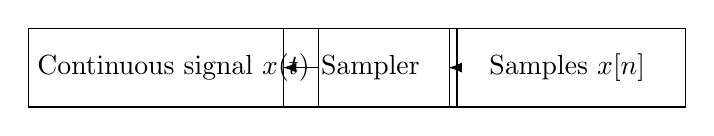
\begin{tikzpicture}[node distance=2.5cm,>=Latex]
\node[draw,minimum width=2.8cm,minimum height=1cm] (x) {Continuous signal $x(t)$};
\node[draw,minimum width=2.2cm,minimum height=1cm,right of=x] (s) {Sampler};
\node[draw,minimum width=3cm,minimum height=1cm,right of=s] (xs) {Samples $x[n]$};

\draw[->] (x) -- (s);
\draw[->] (s) -- (xs);
\end{tikzpicture}
\end{center}

The central question is:

\begin{center}
\textbf{How fast should we sample a signal so that it can be perfectly reconstructed?}
\end{center}

%%%%%%%%%%%%%%%%%%%%%%%%%%%%%%%%%%%%%%%%%%%%%%%%%%%%%%%%%%%%%%%%%%%%%%%%%%%%%%%%

\section{Sampling Period and Sampling Frequency}

Let

\[
T_s=\text{sampling period (seconds)}
\]

\[
f_s=\text{sampling frequency (samples/second)}
\]

They are related by

\[
\boxed{
f_s=\frac{1}{T_s}
}
\]

%%%%%%%%%%%%%%%%%%%%%%%%%%%%%%%%%%%%%%%%%%%%%%%%%%%%%%%%%%%%%%%%%%%%%%%%%%%%%%%%

\subsection{Example}

If

\[
T_s=1\text{ ms}=10^{-3}\text{ s},
\]

then

\[
f_s=\frac{1}{10^{-3}}=1000\text{ Hz}=1\text{ kHz}.
\]

%%%%%%%%%%%%%%%%%%%%%%%%%%%%%%%%%%%%%%%%%%%%%%%%%%%%%%%%%%%%%%%%%%%%%%%%%%%%%%%%

\section{Discrete-Time Sequence}

Sampling a continuous-time signal at instants

\[
t=nT_s,\qquad n=0,\pm1,\pm2,\ldots
\]

produces the discrete sequence

\[
\boxed{
x[n]=x(nT_s)
}
\]

%%%%%%%%%%%%%%%%%%%%%%%%%%%%%%%%%%%%%%%%%%%%%%%%%%%%%%%%%%%%%%%%%%%%%%%%%%%%%%%%

\section{Impulse Sampling}

Ideal sampling is modeled by multiplying the signal with an impulse train.

%%%%%%%%%%%%%%%%%%%%%%%%%%%%%%%%%%%%%%%%%%%%%%%%%%%%%%%%%%%%%%%%%%%%%%%%%%%%%%%%

\subsection{Impulse Train}

\[
\boxed{
p(t)=\sum_{n=-\infty}^{\infty}\delta(t-nT_s)
}
\]

%%%%%%%%%%%%%%%%%%%%%%%%%%%%%%%%%%%%%%%%%%%%%%%%%%%%%%%%%%%%%%%%%%%%%%%%%%%%%%%%

\subsection{Sampled Signal}

\[
x_s(t)=x(t)p(t)
\]

Substituting \(p(t)\),

\[
\boxed{
x_s(t)=
\sum_{n=-\infty}^{\infty}
x(nT_s)\delta(t-nT_s)
}
\]

Thus, the amplitudes of the impulses are the sample values.

%%%%%%%%%%%%%%%%%%%%%%%%%%%%%%%%%%%%%%%%%%%%%%%%%%%%%%%%%%%%%%%%%%%%%%%%%%%%%%%%

\section{Spectrum of the Impulse Train}

The Fourier transform of the impulse train is another impulse train:

\[
\boxed{
P(\omega)=
\frac{2\pi}{T_s}
\sum_{k=-\infty}^{\infty}
\delta(\omega-k\omega_s)
}
\]

where

\[
\boxed{
\omega_s=\frac{2\pi}{T_s}=2\pi f_s
}
\]

is the sampling angular frequency.

%%%%%%%%%%%%%%%%%%%%%%%%%%%%%%%%%%%%%%%%%%%%%%%%%%%%%%%%%%%%%%%%%%%%%%%%%%%%%%%%

\section{Spectrum of the Sampled Signal}

Since multiplication in time corresponds to convolution in frequency,

\[
X_s(\omega)=
\frac{1}{2\pi}
X(\omega)*P(\omega)
\]

Substituting \(P(\omega)\),

\[
\boxed{
X_s(\omega)=
\frac{1}{T_s}
\sum_{k=-\infty}^{\infty}
X(\omega-k\omega_s)
}
\]

%%%%%%%%%%%%%%%%%%%%%%%%%%%%%%%%%%%%%%%%%%%%%%%%%%%%%%%%%%%%%%%%%%%%%%%%%%%%%%%%

\subsection{Interpretation}

The original spectrum is repeated at

\[
\omega=0,\pm\omega_s,\pm2\omega_s,\ldots
\]

with spacing \(\omega_s\).

%%%%%%%%%%%%%%%%%%%%%%%%%%%%%%%%%%%%%%%%%%%%%%%%%%%%%%%%%%%%%%%%%%%%%%%%%%%%%%%%

\section{Bandlimited Signal}

A signal is bandlimited if

\[
\boxed{
X(\omega)=0,\qquad |\omega|>\omega_m
}
\]

where \(\omega_m\) is the highest frequency present.

Equivalently, in hertz,

\[
f_m=\frac{\omega_m}{2\pi}.
\]

%%%%%%%%%%%%%%%%%%%%%%%%%%%%%%%%%%%%%%%%%%%%%%%%%%%%%%%%%%%%%%%%%%%%%%%%%%%%%%%%

\section{Sampling Theorem}

\begin{tcolorbox}[title=Nyquist Sampling Theorem,colback=yellow!10]

A bandlimited signal with maximum frequency \(f_m\) can be perfectly reconstructed
from its samples if the sampling frequency satisfies

\[
\boxed{
f_s\ge 2f_m
}
\]

The minimum sampling frequency

\[
\boxed{
f_N=2f_m
}
\]

is called the \textbf{Nyquist rate}.

\end{tcolorbox}

%%%%%%%%%%%%%%%%%%%%%%%%%%%%%%%%%%%%%%%%%%%%%%%%%%%%%%%%%%%%%%%%%%%%%%%%%%%%%%%%

\section{Why \(2f_m\)?}

The original spectrum occupies

\[
-f_m\le f\le f_m.
\]

After sampling, copies appear centered at \(\pm f_s\).

To avoid overlap,

\[
f_s-f_m\ge f_m
\]

which gives

\[
\boxed{
f_s\ge2f_m
}
\]

%%%%%%%%%%%%%%%%%%%%%%%%%%%%%%%%%%%%%%%%%%%%%%%%%%%%%%%%%%%%%%%%%%%%%%%%%%%%%%%%

\section{Case 1: Proper Sampling}

If

\[
f_s>2f_m,
\]

the spectral copies are separated.

\begin{center}
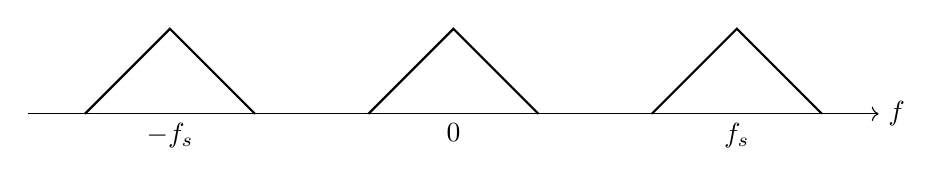
\begin{tikzpicture}[scale=0.9]
\draw[->] (-6,0) -- (6,0) node[right] {$f$};

\draw[thick] (-1.2,0) -- (0,1.2) -- (1.2,0);

\draw[thick] (-5.2,0) -- (-4,1.2) -- (-2.8,0);

\draw[thick] (2.8,0) -- (4,1.2) -- (5.2,0);

\node[below] at (0,0) {$0$};
\node[below] at (4,0) {$f_s$};
\node[below] at (-4,0) {$-f_s$};
\end{tikzpicture}
\end{center}

Perfect reconstruction is possible.

%%%%%%%%%%%%%%%%%%%%%%%%%%%%%%%%%%%%%%%%%%%%%%%%%%%%%%%%%%%%%%%%%%%%%%%%%%%%%%%%

\section{Case 2: Critical Sampling}

If

\[
f_s=2f_m,
\]

the spectra just touch.

This is the theoretical minimum rate.

%%%%%%%%%%%%%%%%%%%%%%%%%%%%%%%%%%%%%%%%%%%%%%%%%%%%%%%%%%%%%%%%%%%%%%%%%%%%%%%%

\section{Case 3: Undersampling}

If

\[
f_s<2f_m,
\]

the spectra overlap.

\begin{center}
\begin{tikzpicture}[scale=0.9]
\draw[->] (-5,0) -- (5,0) node[right] {$f$};

\draw[thick] (-2.2,0) -- (-1,1.2) -- (0.2,0);

\draw[thick] (-0.2,0) -- (1,1.2) -- (2.2,0);

\node[below] at (0,0) {$0$};
\end{tikzpicture}
\end{center}

This phenomenon is called \textbf{aliasing}.

%%%%%%%%%%%%%%%%%%%%%%%%%%%%%%%%%%%%%%%%%%%%%%%%%%%%%%%%%%%%%%%%%%%%%%%%%%%%%%%%

\section{Aliasing}

\subsection{Definition}

Aliasing occurs when different frequency components become indistinguishable after
sampling.

%%%%%%%%%%%%%%%%%%%%%%%%%%%%%%%%%%%%%%%%%%%%%%%%%%%%%%%%%%%%%%%%%%%%%%%%%%%%%%%%

\subsection{Alias Frequency Formula}

For a sinusoid of frequency \(f\),

\[
\boxed{
f_a=\left|f-kf_s\right|
}
\]

where \(k\) is chosen so that \(0\le f_a\le f_s/2\).

%%%%%%%%%%%%%%%%%%%%%%%%%%%%%%%%%%%%%%%%%%%%%%%%%%%%%%%%%%%%%%%%%%%%%%%%%%%%%%%%

\subsection{Example}

Let

\[
f=900\text{ Hz},
\qquad
f_s=1000\text{ Hz}.
\]

Choose \(k=1\):

\[
f_a=|900-1000|=100\text{ Hz}.
\]

So a 900 Hz signal appears as a 100 Hz signal after sampling.

%%%%%%%%%%%%%%%%%%%%%%%%%%%%%%%%%%%%%%%%%%%%%%%%%%%%%%%%%%%%%%%%%%%%%%%%%%%%%%%%

\section{Nyquist Frequency}

The highest frequency that can be represented without aliasing is

\[
\boxed{
f_{max}=\frac{f_s}{2}
}
\]

called the \textbf{Nyquist frequency}.

%%%%%%%%%%%%%%%%%%%%%%%%%%%%%%%%%%%%%%%%%%%%%%%%%%%%%%%%%%%%%%%%%%%%%%%%%%%%%%%%

\section{Anti-Aliasing Filter}

Before sampling, the signal is passed through a low-pass filter to remove frequency
components above \(f_s/2\).

\begin{center}
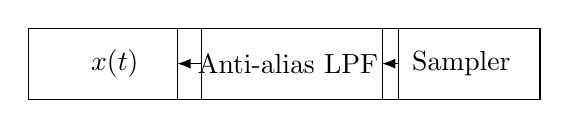
\begin{tikzpicture}[node distance=2.2cm,>=Latex]
\node[draw,minimum width=2.2cm,minimum height=0.9cm] (x) {$x(t)$};
\node[draw,minimum width=2.8cm,minimum height=0.9cm,right of=x] (lpf) {Anti-alias LPF};
\node[draw,minimum width=2cm,minimum height=0.9cm,right of=lpf] (s) {Sampler};

\draw[->] (x) -- (lpf);
\draw[->] (lpf) -- (s);
\end{tikzpicture}
\end{center}

%%%%%%%%%%%%%%%%%%%%%%%%%%%%%%%%%%%%%%%%%%%%%%%%%%%%%%%%%%%%%%%%%%%%%%%%%%%%%%%%

\section{Ideal Reconstruction}

If \(f_s\ge2f_m\), the original signal can be recovered by an ideal low-pass filter.

%%%%%%%%%%%%%%%%%%%%%%%%%%%%%%%%%%%%%%%%%%%%%%%%%%%%%%%%%%%%%%%%%%%%%%%%%%%%%%%%

\subsection{Reconstruction Filter}

\[
\boxed{
H_r(\omega)=
\begin{cases}
T_s, & |\omega|\le\omega_m\\
0, & |\omega|>\omega_m
\end{cases}
}
\]

The filter passes the baseband copy and rejects all other spectral replicas.

%%%%%%%%%%%%%%%%%%%%%%%%%%%%%%%%%%%%%%%%%%%%%%%%%%%%%%%%%%%%%%%%%%%%%%%%%%%%%%%%

\section{Reconstruction Formula}

The reconstructed signal is

\[
x(t)=
\sum_{n=-\infty}^{\infty}
x(nT_s)\,
\mathrm{sinc}\left(\frac{t-nT_s}{T_s}\right)
\]

where

\[
\boxed{
\mathrm{sinc}(x)=\frac{\sin(\pi x)}{\pi x}
}
\]

This is the \textbf{sinc interpolation formula}.

%%%%%%%%%%%%%%%%%%%%%%%%%%%%%%%%%%%%%%%%%%%%%%%%%%%%%%%%%%%%%%%%%%%%%%%%%%%%%%%%

\section{Worked Example 6.1}

A signal contains frequencies up to

\[
f_m=5\text{ kHz}.
\]

Find the Nyquist rate and the minimum sampling period.

%%%%%%%%%%%%%%%%%%%%%%%%%%%%%%%%%%%%%%%%%%%%%%%%%%%%%%%%%%%%%%%%%%%%%%%%%%%%%%%%

\subsection{Solution}

\[
f_N=2f_m=10\text{ kHz}
\]

\[
T_s=\frac{1}{f_N}
=\frac{1}{10^4}
=100\ \mu s
\]

\[
\boxed{
f_N=10\text{ kHz},
\qquad
T_s=100\ \mu s
}
\]

%%%%%%%%%%%%%%%%%%%%%%%%%%%%%%%%%%%%%%%%%%%%%%%%%%%%%%%%%%%%%%%%%%%%%%%%%%%%%%%%

\section{Worked Example 6.2}

A signal is sampled at

\[
f_s=8\text{ kHz}.
\]

What is the maximum frequency that can be represented without aliasing?

%%%%%%%%%%%%%%%%%%%%%%%%%%%%%%%%%%%%%%%%%%%%%%%%%%%%%%%%%%%%%%%%%%%%%%%%%%%%%%%%

\subsection{Solution}

\[
f_{max}=\frac{f_s}{2}=4\text{ kHz}
\]

\[
\boxed{
f_{max}=4\text{ kHz}
}
\]

%%%%%%%%%%%%%%%%%%%%%%%%%%%%%%%%%%%%%%%%%%%%%%%%%%%%%%%%%%%%%%%%%%%%%%%%%%%%%%%%

\section{Worked Example 6.3}

A 6 kHz sinusoid is sampled at 8 kHz. Find the alias frequency.

%%%%%%%%%%%%%%%%%%%%%%%%%%%%%%%%%%%%%%%%%%%%%%%%%%%%%%%%%%%%%%%%%%%%%%%%%%%%%%%%

\subsection{Solution}

\[
f_a=|6-8|=2\text{ kHz}
\]

\[
\boxed{
f_a=2\text{ kHz}
}
\]

%%%%%%%%%%%%%%%%%%%%%%%%%%%%%%%%%%%%%%%%%%%%%%%%%%%%%%%%%%%%%%%%%%%%%%%%%%%%%%%%

\begin{tcolorbox}[title=Quick Recall,colback=blue!5]

\[
f_s=\frac{1}{T_s}
\]

\[
\omega_s=2\pi f_s
\]

\[
X_s(\omega)=
\frac{1}{T_s}
\sum_{k=-\infty}^{\infty}
X(\omega-k\omega_s)
\]

\[
f_s\ge2f_m
\]

\[
f_N=2f_m
\]

\[
f_{max}=\frac{f_s}{2}
\]

\[
f_a=|f-kf_s|
\]

\[
x(t)=
\sum_{n=-\infty}^{\infty}
x(nT_s)\,
\mathrm{sinc}\left(\frac{t-nT_s}{T_s}\right)
\]

\end{tcolorbox}
%%%%%%%%%%%%%%%%%%%%%%%%%%%%%%%%%%%%%%%%%%%%%%%%%%%%%%%%%%%%%%%%%%%%%%%%%%%%%%%%
%%%%%%%%%%%%%%%%%%%%%%%%%%%%%%%%%%%%%%%%%%%%%%%%%%%%%%%%%%%%%%%%%%%%%%%%%%%%%%%%
\section{Proof of the Sampling Theorem}

Assume \(x(t)\) is bandlimited:

\[
X(\omega)=0,\qquad |\omega|>\omega_m
\]

After sampling,

\[
X_s(\omega)=
\frac{1}{T_s}
\sum_{k=-\infty}^{\infty}
X(\omega-k\omega_s)
\]

The replicas are centered at

\[
0,\pm\omega_s,\pm2\omega_s,\ldots
\]

For perfect reconstruction, adjacent replicas must not overlap.

%%%%%%%%%%%%%%%%%%%%%%%%%%%%%%%%%%%%%%%%%%%%%%%%%%%%%%%%%%%%%%%%%%%%%%%%%%%%%%%%

\subsection{Condition}

The right edge of the baseband spectrum is \(\omega_m\).

The left edge of the first shifted replica is \(\omega_s-\omega_m\).

Require

\[
\omega_s-\omega_m\ge\omega_m
\]

Hence,

\[
\boxed{
\omega_s\ge2\omega_m
}
\]

Dividing by \(2\pi\),

\[
\boxed{
f_s\ge2f_m
}
\]

Thus, the Nyquist theorem is proved.

%%%%%%%%%%%%%%%%%%%%%%%%%%%%%%%%%%%%%%%%%%%%%%%%%%%%%%%%%%%%%%%%%%%%%%%%%%%%%%%%

\section{Natural Sampling}

In natural sampling, the switch remains ON for a short duration \(\tau\).

%%%%%%%%%%%%%%%%%%%%%%%%%%%%%%%%%%%%%%%%%%%%%%%%%%%%%%%%%%%%%%%%%%%%%%%%%%%%%%%%

\subsection{Waveform}

\begin{center}
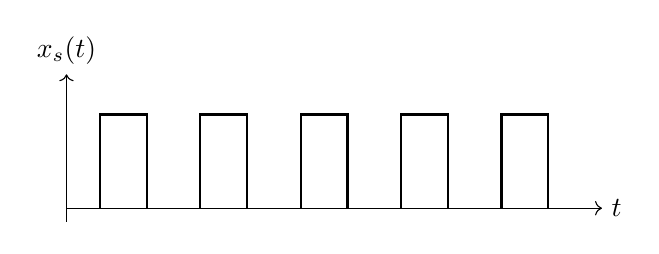
\begin{tikzpicture}[scale=0.85]
\draw[->] (0,0) -- (8,0) node[right] {$t$};
\draw[->] (0,-0.2) -- (0,2) node[above] {$x_s(t)$};

\foreach \x in {0.5,2,3.5,5,6.5}{
  \draw[thick] (\x,0) -- (\x,1.4) -- ++(0.7,0) -- ++(0,-1.4);
}
\end{tikzpicture}
\end{center}

The top of each pulse follows the original signal shape.

%%%%%%%%%%%%%%%%%%%%%%%%%%%%%%%%%%%%%%%%%%%%%%%%%%%%%%%%%%%%%%%%%%%%%%%%%%%%%%%%

\section{Flat-Top Sampling}

In practical sample-and-hold circuits, the sampled value is held constant during the pulse width.

%%%%%%%%%%%%%%%%%%%%%%%%%%%%%%%%%%%%%%%%%%%%%%%%%%%%%%%%%%%%%%%%%%%%%%%%%%%%%%%%

\subsection{Waveform}

\begin{center}
\begin{tikzpicture}[scale=0.85]
\draw[->] (0,0) -- (8,0) node[right] {$t$};
\draw[->] (0,-0.2) -- (0,2) node[above] {$x_s(t)$};

\draw[thick] (0.5,0) -- (0.5,0.8) -- (1.2,0.8) -- (1.2,0);
\draw[thick] (2,0) -- (2,1.3) -- (2.7,1.3) -- (2.7,0);
\draw[thick] (3.5,0) -- (3.5,0.6) -- (4.2,0.6) -- (4.2,0);
\draw[thick] (5,0) -- (5,1.5) -- (5.7,1.5) -- (5.7,0);
\end{tikzpicture}
\end{center}

This is the most common practical sampling method.

%%%%%%%%%%%%%%%%%%%%%%%%%%%%%%%%%%%%%%%%%%%%%%%%%%%%%%%%%%%%%%%%%%%%%%%%%%%%%%%%

\section{Aperture Effect}

Because the sample is averaged over a finite pulse width \(\tau\), high-frequency
components are attenuated.

%%%%%%%%%%%%%%%%%%%%%%%%%%%%%%%%%%%%%%%%%%%%%%%%%%%%%%%%%%%%%%%%%%%%%%%%%%%%%%%%

\subsection{Frequency Response}

\[
\boxed{
H_a(\omega)=
\tau\,\mathrm{sinc}\left(\frac{\omega\tau}{2}\right)
e^{-j\omega\tau/2}
}
\]

The magnitude response is

\[
|H_a(\omega)|=
\tau\left|
\mathrm{sinc}\left(\frac{\omega\tau}{2}\right)
\right|
\]

%%%%%%%%%%%%%%%%%%%%%%%%%%%%%%%%%%%%%%%%%%%%%%%%%%%%%%%%%%%%%%%%%%%%%%%%%%%%%%%%

\subsection{Consequence}

\begin{itemize}
\item Low frequencies are almost unaffected.
\item High frequencies are attenuated.
\item This produces amplitude distortion.
\end{itemize}

%%%%%%%%%%%%%%%%%%%%%%%%%%%%%%%%%%%%%%%%%%%%%%%%%%%%%%%%%%%%%%%%%%%%%%%%%%%%%%%%

\section{Oversampling}

Oversampling means

\[
\boxed{
f_s\gg2f_m
}
\]

%%%%%%%%%%%%%%%%%%%%%%%%%%%%%%%%%%%%%%%%%%%%%%%%%%%%%%%%%%%%%%%%%%%%%%%%%%%%%%%%

\subsection{Advantages}

\begin{itemize}
\item Easier anti-aliasing filter design.
\item Reduced quantization noise in the signal band.
\item Better signal-to-noise ratio after digital filtering.
\end{itemize}

%%%%%%%%%%%%%%%%%%%%%%%%%%%%%%%%%%%%%%%%%%%%%%%%%%%%%%%%%%%%%%%%%%%%%%%%%%%%%%%%

\subsection{Example}

Audio signals are often sampled at

\[
44.1\text{ kHz}
\]

even though human hearing is limited to about

\[
20\text{ kHz}.
\]

%%%%%%%%%%%%%%%%%%%%%%%%%%%%%%%%%%%%%%%%%%%%%%%%%%%%%%%%%%%%%%%%%%%%%%%%%%%%%%%%

\section{Undersampling}

If

\[
f_s<2f_m,
\]

aliasing occurs.

%%%%%%%%%%%%%%%%%%%%%%%%%%%%%%%%%%%%%%%%%%%%%%%%%%%%%%%%%%%%%%%%%%%%%%%%%%%%%%%%

\subsection{Example}

A 7 kHz signal sampled at 10 kHz gives

\[
f_a=|7-10|=3\text{ kHz}
\]

The reconstructed signal contains a false 3 kHz component.

%%%%%%%%%%%%%%%%%%%%%%%%%%%%%%%%%%%%%%%%%%%%%%%%%%%%%%%%%%%%%%%%%%%%%%%%%%%%%%%%

\section{Bandpass Sampling}

If a signal occupies a band

\[
f_L\le f\le f_H,
\]

it is sometimes possible to sample below \(2f_H\).

%%%%%%%%%%%%%%%%%%%%%%%%%%%%%%%%%%%%%%%%%%%%%%%%%%%%%%%%%%%%%%%%%%%%%%%%%%%%%%%%

\subsection{Condition}

For an integer \(n\),

\[
\boxed{
\frac{2f_H}{n}
\le
f_s
\le
\frac{2f_L}{n-1}
}
\]

This technique is widely used in radio receivers.

%%%%%%%%%%%%%%%%%%%%%%%%%%%%%%%%%%%%%%%%%%%%%%%%%%%%%%%%%%%%%%%%%%%%%%%%%%%%%%%%

\section{Example of Bandpass Sampling}

Suppose

\[
f_L=90\text{ MHz},
\qquad
f_H=100\text{ MHz}.
\]

The signal bandwidth is

\[
B=10\text{ MHz}.
\]

Instead of sampling at

\[
200\text{ MHz},
\]

a suitable lower sampling frequency can be chosen using the bandpass sampling
condition.

%%%%%%%%%%%%%%%%%%%%%%%%%%%%%%%%%%%%%%%%%%%%%%%%%%%%%%%%%%%%%%%%%%%%%%%%%%%%%%%%

\section{Reconstruction Filter}

The ideal reconstruction filter has cutoff

\[
\omega_c=\omega_m.
\]

Its frequency response is

\[
H_r(\omega)=
\begin{cases}
T_s, & |\omega|\le\omega_m\\
0, & |\omega|>\omega_m
\end{cases}
\]

%%%%%%%%%%%%%%%%%%%%%%%%%%%%%%%%%%%%%%%%%%%%%%%%%%%%%%%%%%%%%%%%%%%%%%%%%%%%%%%%

\subsection{Why Gain \(T_s\)?}

The sampled spectrum is scaled by \(1/T_s\).

The reconstruction filter multiplies it by \(T_s\), restoring the original amplitude.

%%%%%%%%%%%%%%%%%%%%%%%%%%%%%%%%%%%%%%%%%%%%%%%%%%%%%%%%%%%%%%%%%%%%%%%%%%%%%%%%

\section{Sinc Interpolation}

The reconstructed signal is

\[
\boxed{
x(t)=
\sum_{n=-\infty}^{\infty}
x(nT_s)\,
\mathrm{sinc}\left(\frac{t-nT_s}{T_s}\right)
}
\]

Each sample generates a shifted sinc pulse, and the sum of all sinc pulses
reconstructs the original signal exactly.

%%%%%%%%%%%%%%%%%%%%%%%%%%%%%%%%%%%%%%%%%%%%%%%%%%%%%%%%%%%%%%%%%%%%%%%%%%%%%%%%

\section{Why Sinc Passes Through the Samples}

Since

\[
\mathrm{sinc}(0)=1
\]

and

\[
\mathrm{sinc}(k)=0,\qquad k=\pm1,\pm2,\ldots
\]

at \(t=mT_s\),

\[
x(mT_s)=x[m].
\]

Thus, the interpolation passes through every sample point.

%%%%%%%%%%%%%%%%%%%%%%%%%%%%%%%%%%%%%%%%%%%%%%%%%%%%%%%%%%%%%%%%%%%%%%%%%%%%%%%%

\section{Solved Example 6.4}

A signal has maximum frequency

\[
f_m=12\text{ kHz}.
\]

Find the Nyquist rate, minimum sampling period, and a practical sampling frequency.

%%%%%%%%%%%%%%%%%%%%%%%%%%%%%%%%%%%%%%%%%%%%%%%%%%%%%%%%%%%%%%%%%%%%%%%%%%%%%%%%

\subsection{Solution}

Nyquist rate:

\[
f_N=2f_m=24\text{ kHz}
\]

Minimum sampling period:

\[
T_s=\frac{1}{24\times10^3}=41.67\ \mu s
\]

A practical choice is

\[
\boxed{
f_s=30\text{ kHz}
}
\]

%%%%%%%%%%%%%%%%%%%%%%%%%%%%%%%%%%%%%%%%%%%%%%%%%%%%%%%%%%%%%%%%%%%%%%%%%%%%%%%%

\section{Solved Example 6.5}

A 15 kHz signal is sampled at 20 kHz. Determine the alias frequency.

%%%%%%%%%%%%%%%%%%%%%%%%%%%%%%%%%%%%%%%%%%%%%%%%%%%%%%%%%%%%%%%%%%%%%%%%%%%%%%%%

\subsection{Solution}

\[
f_a=|15-20|=5\text{ kHz}
\]

\[
\boxed{
f_a=5\text{ kHz}
}
\]

%%%%%%%%%%%%%%%%%%%%%%%%%%%%%%%%%%%%%%%%%%%%%%%%%%%%%%%%%%%%%%%%%%%%%%%%%%%%%%%%

\section{Solved Example 6.6}

A signal contains frequencies up to 3 kHz and is sampled at 6 kHz. Is perfect
reconstruction possible?

%%%%%%%%%%%%%%%%%%%%%%%%%%%%%%%%%%%%%%%%%%%%%%%%%%%%%%%%%%%%%%%%%%%%%%%%%%%%%%%%

\subsection{Solution}

\[
f_s=6\text{ kHz},
\qquad
2f_m=6\text{ kHz}
\]

Since

\[
f_s=2f_m,
\]

the signal is sampled at the Nyquist rate.

\[
\boxed{
\text{Yes, perfect reconstruction is theoretically possible.}
}
\]

In practice, a slightly higher sampling frequency is preferred.

%%%%%%%%%%%%%%%%%%%%%%%%%%%%%%%%%%%%%%%%%%%%%%%%%%%%%%%%%%%%%%%%%%%%%%%%%%%%%%%%

\section{Solved Example 6.7}

A signal is sampled at 48 kHz. What is the Nyquist frequency?

%%%%%%%%%%%%%%%%%%%%%%%%%%%%%%%%%%%%%%%%%%%%%%%%%%%%%%%%%%%%%%%%%%%%%%%%%%%%%%%%

\subsection{Solution}

\[
f_N=\frac{48}{2}=24\text{ kHz}
\]

\[
\boxed{
f_N=24\text{ kHz}
}
\]

%%%%%%%%%%%%%%%%%%%%%%%%%%%%%%%%%%%%%%%%%%%%%%%%%%%%%%%%%%%%%%%%%%%%%%%%%%%%%%%%

\section{Practical ADC Chain}

\begin{center}
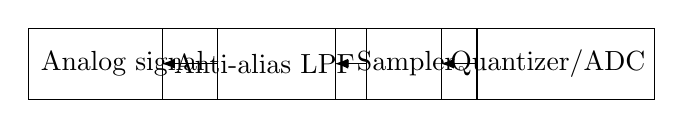
\begin{tikzpicture}[node distance=1.8cm,>=Latex]
\node[draw,minimum width=2.4cm,minimum height=0.9cm] (x) {Analog signal};
\node[draw,minimum width=2.6cm,minimum height=0.9cm,right of=x] (lpf) {Anti-alias LPF};
\node[draw,minimum width=1.8cm,minimum height=0.9cm,right of=lpf] (s) {Sampler};
\node[draw,minimum width=2.2cm,minimum height=0.9cm,right of=s] (adc) {Quantizer/ADC};

\draw[->] (x) -- (lpf);
\draw[->] (lpf) -- (s);
\draw[->] (s) -- (adc);
\end{tikzpicture}
\end{center}

The anti-alias filter is essential before the sampler.

%%%%%%%%%%%%%%%%%%%%%%%%%%%%%%%%%%%%%%%%%%%%%%%%%%%%%%%%%%%%%%%%%%%%%%%%%%%%%%%%

\section{Comparison of Sampling Methods}

\begin{table}[H]
\centering
\caption{Sampling methods}
\begin{tabular}{|p{4cm}|p{5cm}|p{3cm}|}
\hline
\textbf{Method} & \textbf{Pulse Shape} & \textbf{Practical?}\\
\hline
Ideal sampling & Impulses & No\\
\hline
Natural sampling & Signal-shaped pulses & Limited\\
\hline
Flat-top sampling & Constant pulses & Yes\\
\hline
\end{tabular}
\end{table}

%%%%%%%%%%%%%%%%%%%%%%%%%%%%%%%%%%%%%%%%%%%%%%%%%%%%%%%%%%%%%%%%%%%%%%%%%%%%%%%%

\section{Common GATE Mistakes}

\begin{enumerate}
\item Using \(f_s=f_m\) instead of \(2f_m\).
\item Forgetting that Nyquist frequency is \(f_s/2\).
\item Using the wrong value of \(k\) in alias calculations.
\item Confusing sampling rate with signal frequency.
\item Ignoring the anti-aliasing filter.
\item Forgetting the scaling factor \(T_s\) in reconstruction.
\item Using \(\sin x/x\) without normalizing the sinc function.
\end{enumerate}

%%%%%%%%%%%%%%%%%%%%%%%%%%%%%%%%%%%%%%%%%%%%%%%%%%%%%%%%%%%%%%%%%%%%%%%%%%%%%%%%

\section{Chapter Summary}

In this chapter, we studied the sampling process and showed that sampling
creates periodic replicas of the signal spectrum. By preventing overlap between
these replicas, we obtained the Nyquist condition

\[
f_s\ge2f_m.
\]

We also studied aliasing, anti-aliasing filters, practical sampling methods,
aperture effect, oversampling, undersampling and bandpass sampling.

Finally, we learned that an ideally sampled signal can be perfectly reconstructed
using sinc interpolation and an ideal low-pass filter.

%%%%%%%%%%%%%%%%%%%%%%%%%%%%%%%%%%%%%%%%%%%%%%%%%%%%%%%%%%%%%%%%%%%%%%%%%%%%%%%%

\begin{tcolorbox}[title=One-Minute Revision,colback=blue!5]

\[
f_s=\frac{1}{T_s}
\]

\[
\omega_s=2\pi f_s
\]

\[
X_s(\omega)=
\frac{1}{T_s}
\sum_{k=-\infty}^{\infty}
X(\omega-k\omega_s)
\]

\[
f_s\ge2f_m
\]

\[
f_N=2f_m
\]

\[
f_{max}=\frac{f_s}{2}
\]

\[
f_a=|f-kf_s|
\]

\[
x(t)=
\sum_{n=-\infty}^{\infty}
x[n]\,
\mathrm{sinc}\left(\frac{t-nT_s}{T_s}\right)
\]

Ideal LPF cutoff:

\[
\omega_c=\omega_m
\]

Bandpass sampling:

\[
\frac{2f_H}{n}
\le
f_s
\le
\frac{2f_L}{n-1}
\]

\end{tcolorbox}
%%%%%%%%%%%%%%%%%%%%%%%%%%%%%%%%%%%%%%%%%%%%%%%%%%%%%%%%%%%%%%%%%%%%%%%%%%%%%%%%
%%%%%%%%%%%%%%%%%%%%%%%%%%%%%%%%%%%%%%%%%%%%%%%%%%%%%%%%%%%%%%%%%%%%%%%%%%%%%%%%
% CHAPTER 7
%%%%%%%%%%%%%%%%%%%%%%%%%%%%%%%%%%%%%%%%%%%%%%%%%%%%%%%%%%%%%%%%%%%%%%%%%%%%%%%%

\chapter{Discrete-Time Signals and Systems}

\begin{tcolorbox}[colback=blue!5!white,colframe=blue!70!black,title=Learning Objectives]

After studying this chapter, the reader will be able to

\begin{itemize}
\item Define discrete-time signals and sequences.
\item Understand basic sequence operations.
\item Define discrete-time systems.
\item Test linearity, time invariance, causality and stability.
\item Understand discrete-time convolution.
\item Compute the output of an LTI discrete-time system.
\end{itemize}

\end{tcolorbox}

%%%%%%%%%%%%%%%%%%%%%%%%%%%%%%%%%%%%%%%%%%%%%%%%%%%%%%%%%%%%%%%%%%%%%%%%%%%%%%%%

\section{Introduction}

A \textbf{discrete-time signal} is a signal defined only at discrete instants of time.

Instead of \(x(t)\), we use the notation

\[
\boxed{
x[n]
}
\]

where \(n\) is an integer.

Discrete-time signals arise naturally from sampling continuous-time signals and are
the basic signals processed by digital computers, DSP processors and microcontrollers.

%%%%%%%%%%%%%%%%%%%%%%%%%%%%%%%%%%%%%%%%%%%%%%%%%%%%%%%%%%%%%%%%%%%%%%%%%%%%%%%%

\section{Continuous-Time vs Discrete-Time}

\begin{table}[H]
\centering
\caption{Comparison of signal types}
\begin{tabular}{|p{4cm}|p{4cm}|p{4cm}|}
\hline
\textbf{Feature} & \textbf{Continuous-Time} & \textbf{Discrete-Time}\\
\hline
Independent variable & \(t\) & \(n\)\\
\hline
Definition & All real values & Integer values only\\
\hline
Notation & \(x(t)\) & \(x[n]\)\\
\hline
Example & \(\sin(2\pi t)\) & \(\sin(0.2\pi n)\)\\
\hline
\end{tabular}
\end{table}

%%%%%%%%%%%%%%%%%%%%%%%%%%%%%%%%%%%%%%%%%%%%%%%%%%%%%%%%%%%%%%%%%%%%%%%%%%%%%%%%

\section{Sampling Relationship}

If a continuous-time signal is sampled every \(T_s\) seconds, then

\[
\boxed{
x[n]=x(nT_s)
}
\]

where

\begin{itemize}
\item \(T_s\): sampling period,
\item \(f_s=1/T_s\): sampling frequency.
\end{itemize}

%%%%%%%%%%%%%%%%%%%%%%%%%%%%%%%%%%%%%%%%%%%%%%%%%%%%%%%%%%%%%%%%%%%%%%%%%%%%%%%%

\section{Basic Sequences}

%%%%%%%%%%%%%%%%%%%%%%%%%%%%%%%%%%%%%%%%%%%%%%%%%%%%%%%%%%%%%%%%%%%%%%%%%%%%%%%%

\subsection{Unit Sample Sequence}

\[
\boxed{
\delta[n]=
\begin{cases}
1, & n=0\\
0, & n\neq0
\end{cases}
}
\]

%%%%%%%%%%%%%%%%%%%%%%%%%%%%%%%%%%%%%%%%%%%%%%%%%%%%%%%%%%%%%%%%%%%%%%%%%%%%%%%%

\subsection{Unit Step Sequence}

\[
\boxed{
u[n]=
\begin{cases}
1, & n\ge0\\
0, & n<0
\end{cases}
}
\]

%%%%%%%%%%%%%%%%%%%%%%%%%%%%%%%%%%%%%%%%%%%%%%%%%%%%%%%%%%%%%%%%%%%%%%%%%%%%%%%%

\subsection{Exponential Sequence}

\[
\boxed{
x[n]=a^n u[n]
}
\]

\begin{itemize}
\item \(|a|<1\): decaying,
\item \(|a|>1\): growing,
\item \(a<0\): alternating sign.
\end{itemize}

%%%%%%%%%%%%%%%%%%%%%%%%%%%%%%%%%%%%%%%%%%%%%%%%%%%%%%%%%%%%%%%%%%%%%%%%%%%%%%%%

\section{Sequence Operations}

%%%%%%%%%%%%%%%%%%%%%%%%%%%%%%%%%%%%%%%%%%%%%%%%%%%%%%%%%%%%%%%%%%%%%%%%%%%%%%%%

\subsection{Time Shifting}

Delay by \(n_0\):

\[
\boxed{
x[n-n_0]
}
\]

Advance by \(n_0\):

\[
\boxed{
x[n+n_0]
}
\]

%%%%%%%%%%%%%%%%%%%%%%%%%%%%%%%%%%%%%%%%%%%%%%%%%%%%%%%%%%%%%%%%%%%%%%%%%%%%%%%%

\subsection{Time Reversal}

\[
\boxed{
x[-n]
}
\]

%%%%%%%%%%%%%%%%%%%%%%%%%%%%%%%%%%%%%%%%%%%%%%%%%%%%%%%%%%%%%%%%%%%%%%%%%%%%%%%%

\subsection{Amplitude Scaling}

\[
\boxed{
y[n]=A\,x[n]
}
\]

%%%%%%%%%%%%%%%%%%%%%%%%%%%%%%%%%%%%%%%%%%%%%%%%%%%%%%%%%%%%%%%%%%%%%%%%%%%%%%%%

\section{Even and Odd Sequences}

%%%%%%%%%%%%%%%%%%%%%%%%%%%%%%%%%%%%%%%%%%%%%%%%%%%%%%%%%%%%%%%%%%%%%%%%%%%%%%%%

\subsection{Even Sequence}

\[
\boxed{
x[n]=x[-n]
}
\]

%%%%%%%%%%%%%%%%%%%%%%%%%%%%%%%%%%%%%%%%%%%%%%%%%%%%%%%%%%%%%%%%%%%%%%%%%%%%%%%%

\subsection{Odd Sequence}

\[
\boxed{
x[n]=-x[-n]
}
\]

%%%%%%%%%%%%%%%%%%%%%%%%%%%%%%%%%%%%%%%%%%%%%%%%%%%%%%%%%%%%%%%%%%%%%%%%%%%%%%%%

\subsection{Decomposition}

Any sequence can be written as

\[
\boxed{
x[n]=x_e[n]+x_o[n]
}
\]

where

\[
\boxed{
x_e[n]=\frac{x[n]+x[-n]}{2}
}
\]

and

\[
\boxed{
x_o[n]=\frac{x[n]-x[-n]}{2}
}
\]

%%%%%%%%%%%%%%%%%%%%%%%%%%%%%%%%%%%%%%%%%%%%%%%%%%%%%%%%%%%%%%%%%%%%%%%%%%%%%%%%

\section{Periodic Discrete-Time Signals}

A sequence is periodic if

\[
\boxed{
x[n+N]=x[n]
}
\]

for some positive integer \(N\).

The smallest such integer is the \textbf{fundamental period}.

%%%%%%%%%%%%%%%%%%%%%%%%%%%%%%%%%%%%%%%%%%%%%%%%%%%%%%%%%%%%%%%%%%%%%%%%%%%%%%%%

\subsection{Sinusoidal Sequence}

Consider

\[
x[n]=\cos(\omega_0 n).
\]

It is periodic if

\[
\boxed{
\frac{\omega_0}{2\pi}=\frac{m}{N}
}
\]

where \(m\) and \(N\) are integers.

%%%%%%%%%%%%%%%%%%%%%%%%%%%%%%%%%%%%%%%%%%%%%%%%%%%%%%%%%%%%%%%%%%%%%%%%%%%%%%%%

\subsection{Example}

\[
x[n]=\cos\left(\frac{\pi}{4}n\right)
\]

Here

\[
\frac{\omega_0}{2\pi}=\frac{1}{8}.
\]

Hence,

\[
\boxed{
N=8
}
\]

%%%%%%%%%%%%%%%%%%%%%%%%%%%%%%%%%%%%%%%%%%%%%%%%%%%%%%%%%%%%%%%%%%%%%%%%%%%%%%%%

\section{Discrete-Time Systems}

A discrete-time system maps an input sequence \(x[n]\) to an output sequence
\(y[n]\).

\[
\boxed{
y[n]=T\{x[n]\}
}
\]

%%%%%%%%%%%%%%%%%%%%%%%%%%%%%%%%%%%%%%%%%%%%%%%%%%%%%%%%%%%%%%%%%%%%%%%%%%%%%%%%

\section{Linearity}

A system is linear if

\[
T\{a_1x_1[n]+a_2x_2[n]\}
=
a_1T\{x_1[n]\}+a_2T\{x_2[n]\}.
\]

%%%%%%%%%%%%%%%%%%%%%%%%%%%%%%%%%%%%%%%%%%%%%%%%%%%%%%%%%%%%%%%%%%%%%%%%%%%%%%%%

\subsection{Example}

\[
y[n]=3x[n]-2x[n-1]
\]

is linear.

%%%%%%%%%%%%%%%%%%%%%%%%%%%%%%%%%%%%%%%%%%%%%%%%%%%%%%%%%%%%%%%%%%%%%%%%%%%%%%%%

\section{Time Invariance}

A system is time invariant if delaying the input delays the output by the same amount.

If

\[
x[n]\rightarrow y[n],
\]

then

\[
x[n-n_0]\rightarrow y[n-n_0].
\]

%%%%%%%%%%%%%%%%%%%%%%%%%%%%%%%%%%%%%%%%%%%%%%%%%%%%%%%%%%%%%%%%%%%%%%%%%%%%%%%%

\subsection{Example}

\[
y[n]=x[n]+x[n-1]
\]

is time invariant.

%%%%%%%%%%%%%%%%%%%%%%%%%%%%%%%%%%%%%%%%%%%%%%%%%%%%%%%%%%%%%%%%%%%%%%%%%%%%%%%%

\section{Causality}

A system is causal if the output at time \(n\) depends only on present and past inputs.

%%%%%%%%%%%%%%%%%%%%%%%%%%%%%%%%%%%%%%%%%%%%%%%%%%%%%%%%%%%%%%%%%%%%%%%%%%%%%%%%

\subsection{Causal}

\[
y[n]=x[n]+x[n-2]
\]

%%%%%%%%%%%%%%%%%%%%%%%%%%%%%%%%%%%%%%%%%%%%%%%%%%%%%%%%%%%%%%%%%%%%%%%%%%%%%%%%

\subsection{Noncausal}

\[
y[n]=x[n+1]
\]

because it depends on a future input.

%%%%%%%%%%%%%%%%%%%%%%%%%%%%%%%%%%%%%%%%%%%%%%%%%%%%%%%%%%%%%%%%%%%%%%%%%%%%%%%%

\section{BIBO Stability}

A discrete-time system is stable if every bounded input produces a bounded output.

For an LTI system with impulse response \(h[n]\),

\[
\boxed{
\sum_{n=-\infty}^{\infty}|h[n]|<\infty
}
\]

%%%%%%%%%%%%%%%%%%%%%%%%%%%%%%%%%%%%%%%%%%%%%%%%%%%%%%%%%%%%%%%%%%%%%%%%%%%%%%%%

\section{Impulse Response}

The response to the unit sample sequence is called the impulse response.

\[
\boxed{
h[n]=T\{\delta[n]\}
}
\]

For LTI systems, \(h[n]\) completely characterizes the system.

%%%%%%%%%%%%%%%%%%%%%%%%%%%%%%%%%%%%%%%%%%%%%%%%%%%%%%%%%%%%%%%%%%%%%%%%%%%%%%%%

\section{Convolution Sum}

For a discrete-time LTI system,

\[
\boxed{
y[n]=x[n]*h[n]
}
\]

where

\[
\boxed{
y[n]=
\sum_{k=-\infty}^{\infty}
x[k]\,h[n-k]
}
\]

This is the discrete-time convolution sum.

%%%%%%%%%%%%%%%%%%%%%%%%%%%%%%%%%%%%%%%%%%%%%%%%%%%%%%%%%%%%%%%%%%%%%%%%%%%%%%%%

\section{Graphical Steps for Convolution}

To compute \(y[n]\):

\begin{enumerate}
\item Flip \(h[k]\rightarrow h[-k]\),
\item Shift \(h[-k]\rightarrow h[n-k]\),
\item Multiply \(x[k]\) and \(h[n-k]\),
\item Sum over all \(k\).
\end{enumerate}

%%%%%%%%%%%%%%%%%%%%%%%%%%%%%%%%%%%%%%%%%%%%%%%%%%%%%%%%%%%%%%%%%%%%%%%%%%%%%%%%

\section{Example 1}

Let

\[
x[n]=u[n],
\qquad
h[n]=u[n].
\]

Then

\[
y[n]=
\sum_{k=-\infty}^{\infty}
u[k]u[n-k].
\]

The terms are nonzero when

\[
k\ge0
\]

and

\[
k\le n.
\]

Hence,

\[
y[n]=
\sum_{k=0}^{n}1
=
n+1.
\]

Therefore,

\[
\boxed{
u[n]*u[n]=(n+1)u[n]
}
\]

%%%%%%%%%%%%%%%%%%%%%%%%%%%%%%%%%%%%%%%%%%%%%%%%%%%%%%%%%%%%%%%%%%%%%%%%%%%%%%%%

\section{Example 2}

Let

\[
x[n]=\delta[n]+\delta[n-1],
\]

\[
h[n]=\delta[n]+\delta[n-1].
\]

Using convolution,

\[
y[n]=
\delta[n]
+2\delta[n-1]
+\delta[n-2].
\]

%%%%%%%%%%%%%%%%%%%%%%%%%%%%%%%%%%%%%%%%%%%%%%%%%%%%%%%%%%%%%%%%%%%%%%%%%%%%%%%%

\section{Properties of Convolution}

%%%%%%%%%%%%%%%%%%%%%%%%%%%%%%%%%%%%%%%%%%%%%%%%%%%%%%%%%%%%%%%%%%%%%%%%%%%%%%%%

\subsection{Commutative}

\[
\boxed{
x[n]*h[n]=h[n]*x[n]
}
\]

%%%%%%%%%%%%%%%%%%%%%%%%%%%%%%%%%%%%%%%%%%%%%%%%%%%%%%%%%%%%%%%%%%%%%%%%%%%%%%%%

\subsection{Associative}

\[
\boxed{
(x_1*x_2)*x_3=x_1*(x_2*x_3)
}
\]

%%%%%%%%%%%%%%%%%%%%%%%%%%%%%%%%%%%%%%%%%%%%%%%%%%%%%%%%%%%%%%%%%%%%%%%%%%%%%%%%

\subsection{Distributive}

\[
\boxed{
x*(h_1+h_2)=x*h_1+x*h_2
}
\]

%%%%%%%%%%%%%%%%%%%%%%%%%%%%%%%%%%%%%%%%%%%%%%%%%%%%%%%%%%%%%%%%%%%%%%%%%%%%%%%%

\section{Difference Equation Representation}

Many discrete-time systems are described by difference equations.

%%%%%%%%%%%%%%%%%%%%%%%%%%%%%%%%%%%%%%%%%%%%%%%%%%%%%%%%%%%%%%%%%%%%%%%%%%%%%%%%

\subsection{First-Order System}

\[
\boxed{
y[n]-ay[n-1]=x[n]
}
\]

where \(a\) is a constant.

This is the discrete-time counterpart of a first-order differential equation.

%%%%%%%%%%%%%%%%%%%%%%%%%%%%%%%%%%%%%%%%%%%%%%%%%%%%%%%%%%%%%%%%%%%%%%%%%%%%%%%%

\section{Finding the Impulse Response}

Apply

\[
x[n]=\delta[n].
\]

Then

\[
h[n]-ah[n-1]=\delta[n].
\]

Solving recursively gives

\[
\boxed{
h[n]=a^n u[n]
}
\]

%%%%%%%%%%%%%%%%%%%%%%%%%%%%%%%%%%%%%%%%%%%%%%%%%%%%%%%%%%%%%%%%%%%%%%%%%%%%%%%%

\section{Memoryless Systems}

A system is memoryless if

\[
y[n]
\]

depends only on

\[
x[n].
\]

%%%%%%%%%%%%%%%%%%%%%%%%%%%%%%%%%%%%%%%%%%%%%%%%%%%%%%%%%%%%%%%%%%%%%%%%%%%%%%%%

\subsection{Example}

\[
y[n]=5x[n]
\]

is memoryless.

%%%%%%%%%%%%%%%%%%%%%%%%%%%%%%%%%%%%%%%%%%%%%%%%%%%%%%%%%%%%%%%%%%%%%%%%%%%%%%%%

\subsection{With Memory}

\[
y[n]=x[n]+x[n-1]
\]

has memory.

%%%%%%%%%%%%%%%%%%%%%%%%%%%%%%%%%%%%%%%%%%%%%%%%%%%%%%%%%%%%%%%%%%%%%%%%%%%%%%%%

\begin{tcolorbox}[title=Quick Recall,colback=blue!5]

\[
x[n]=x(nT_s)
\]

\[
\delta[n]=
\begin{cases}
1,& n=0\\
0,& n\neq0
\end{cases}
\]

\[
u[n]=
\begin{cases}
1,& n\ge0\\
0,& n<0
\end{cases}
\]

\[
y[n]=
\sum_{k=-\infty}^{\infty}
x[k]h[n-k]
\]

\[
u[n]*u[n]=(n+1)u[n]
\]

Causal:

\[
y[n]\text{ depends on }x[n],x[n-1],x[n-2],\ldots
\]

Stable:

\[
\sum |h[n]|<\infty
\]

\end{tcolorbox}
%%%%%%%%%%%%%%%%%%%%%%%%%%%%%%%%%%%%%%%%%%%%%%%%%%%%%%%%%%%%%%%%%%%%%%%%%%%%%%%%
%%%%%%%%%%%%%%%%%%%%%%%%%%%%%%%%%%%%%%%%%%%%%%%%%%%%%%%%%%%%%%%%%%%%%%%%%%%%%%%%
\section{Discrete-Time Fourier Transform (DTFT)}

For an aperiodic discrete-time sequence \(x[n]\), the frequency-domain
representation is the \textbf{Discrete-Time Fourier Transform (DTFT)}.

%%%%%%%%%%%%%%%%%%%%%%%%%%%%%%%%%%%%%%%%%%%%%%%%%%%%%%%%%%%%%%%%%%%%%%%%%%%%%%%%

\subsection{Definition}

\[
\boxed{
X(e^{j\omega})=
\sum_{n=-\infty}^{\infty}
x[n]e^{-j\omega n}
}
\]

where

\[
-\pi\le\omega\le\pi.
\]

%%%%%%%%%%%%%%%%%%%%%%%%%%%%%%%%%%%%%%%%%%%%%%%%%%%%%%%%%%%%%%%%%%%%%%%%%%%%%%%%

\subsection{Inverse DTFT}

\[
\boxed{
x[n]=
\frac{1}{2\pi}
\int_{-\pi}^{\pi}
X(e^{j\omega})e^{j\omega n}\,d\omega
}
\]

The DTFT is periodic in frequency with period \(2\pi\):

\[
\boxed{
X(e^{j(\omega+2\pi)})=X(e^{j\omega})
}
\]

%%%%%%%%%%%%%%%%%%%%%%%%%%%%%%%%%%%%%%%%%%%%%%%%%%%%%%%%%%%%%%%%%%%%%%%%%%%%%%%%

\section{DTFT of Basic Sequences}

%%%%%%%%%%%%%%%%%%%%%%%%%%%%%%%%%%%%%%%%%%%%%%%%%%%%%%%%%%%%%%%%%%%%%%%%%%%%%%%%

\subsection{Unit Sample}

\[
\boxed{
\delta[n]\xleftrightarrow{\mathcal{F}}1
}
\]

%%%%%%%%%%%%%%%%%%%%%%%%%%%%%%%%%%%%%%%%%%%%%%%%%%%%%%%%%%%%%%%%%%%%%%%%%%%%%%%%

\subsection{Shifted Impulse}

\[
\boxed{
\delta[n-n_0]
\xleftrightarrow{\mathcal{F}}
e^{-j\omega n_0}
}
\]

%%%%%%%%%%%%%%%%%%%%%%%%%%%%%%%%%%%%%%%%%%%%%%%%%%%%%%%%%%%%%%%%%%%%%%%%%%%%%%%%

\subsection{Unit Step}

For \(|a|<1\),

\[
x[n]=a^n u[n]
\]

has DTFT

\[
\boxed{
X(e^{j\omega})=
\frac{1}{1-ae^{-j\omega}}
}
\]

This is one of the most important transform pairs.

%%%%%%%%%%%%%%%%%%%%%%%%%%%%%%%%%%%%%%%%%%%%%%%%%%%%%%%%%%%%%%%%%%%%%%%%%%%%%%%%

\section{Frequency Response of an LTI System}

For an LTI system with impulse response \(h[n]\),

\[
\boxed{
H(e^{j\omega})=
\sum_{n=-\infty}^{\infty}
h[n]e^{-j\omega n}
}
\]

The output spectrum is

\[
\boxed{
Y(e^{j\omega})=
X(e^{j\omega})H(e^{j\omega})
}
\]

%%%%%%%%%%%%%%%%%%%%%%%%%%%%%%%%%%%%%%%%%%%%%%%%%%%%%%%%%%%%%%%%%%%%%%%%%%%%%%%%

\section{Example: Moving Average Filter}

Consider

\[
h[n]=
\begin{cases}
1, & n=0,1\\
0, & \text{otherwise}
\end{cases}
\]

Then

\[
H(e^{j\omega})=
1+e^{-j\omega}
\]

Using Euler’s identity,

\[
H(e^{j\omega})=
2e^{-j\omega/2}\cos\frac{\omega}{2}
\]

Hence,

\[
\boxed{
|H(e^{j\omega})|=2\left|\cos\frac{\omega}{2}\right|
}
\]

and

\[
\boxed{
\angle H(e^{j\omega})=-\frac{\omega}{2}
}
\]

This is a simple low-pass filter.

%%%%%%%%%%%%%%%%%%%%%%%%%%%%%%%%%%%%%%%%%%%%%%%%%%%%%%%%%%%%%%%%%%%%%%%%%%%%%%%%

\section{Difference Equation}

A general linear constant-coefficient difference equation is

\[
\boxed{
\sum_{k=0}^{N}a_k y[n-k]
=
\sum_{k=0}^{M}b_k x[n-k]
}
\]

Taking the DTFT,

\[
\left(
\sum_{k=0}^{N}a_k e^{-j\omega k}
\right)
Y(e^{j\omega})
=
\left(
\sum_{k=0}^{M}b_k e^{-j\omega k}
\right)
X(e^{j\omega})
\]

Therefore,

\[
\boxed{
H(e^{j\omega})=
\frac{\sum_{k=0}^{M}b_k e^{-j\omega k}}
{\sum_{k=0}^{N}a_k e^{-j\omega k}}
}
\]

%%%%%%%%%%%%%%%%%%%%%%%%%%%%%%%%%%%%%%%%%%%%%%%%%%%%%%%%%%%%%%%%%%%%%%%%%%%%%%%%

\section{z-Transform}

The DTFT exists only for some sequences. A more general transform is the
\textbf{z-transform}.

%%%%%%%%%%%%%%%%%%%%%%%%%%%%%%%%%%%%%%%%%%%%%%%%%%%%%%%%%%%%%%%%%%%%%%%%%%%%%%%%

\subsection{Definition}

\[
\boxed{
X(z)=
\sum_{n=-\infty}^{\infty}
x[n]z^{-n}
}
\]

where

\[
z=re^{j\omega}.
\]

%%%%%%%%%%%%%%%%%%%%%%%%%%%%%%%%%%%%%%%%%%%%%%%%%%%%%%%%%%%%%%%%%%%%%%%%%%%%%%%%

\subsection{Region of Convergence (ROC)}

The set of values of \(z\) for which the series converges is called the ROC.

The ROC is essential for determining causality and stability.

%%%%%%%%%%%%%%%%%%%%%%%%%%%%%%%%%%%%%%%%%%%%%%%%%%%%%%%%%%%%%%%%%%%%%%%%%%%%%%%%

\section{z-Transform of \(a^n u[n]\)}

\[
X(z)=
\sum_{n=0}^{\infty}a^n z^{-n}
\]

This is a geometric series:

\[
X(z)=
\frac{1}{1-az^{-1}}
\]

with ROC

\[
\boxed{
|z|>|a|
}
\]

%%%%%%%%%%%%%%%%%%%%%%%%%%%%%%%%%%%%%%%%%%%%%%%%%%%%%%%%%%%%%%%%%%%%%%%%%%%%%%%%

\section{Poles and Zeros}

%%%%%%%%%%%%%%%%%%%%%%%%%%%%%%%%%%%%%%%%%%%%%%%%%%%%%%%%%%%%%%%%%%%%%%%%%%%%%%%%

\subsection{Zero}

A value of \(z\) for which

\[
X(z)=0.
\]

%%%%%%%%%%%%%%%%%%%%%%%%%%%%%%%%%%%%%%%%%%%%%%%%%%%%%%%%%%%%%%%%%%%%%%%%%%%%%%%%

\subsection{Pole}

A value of \(z\) for which

\[
X(z)\to\infty.
\]

%%%%%%%%%%%%%%%%%%%%%%%%%%%%%%%%%%%%%%%%%%%%%%%%%%%%%%%%%%%%%%%%%%%%%%%%%%%%%%%%

\subsection{Example}

\[
X(z)=
\frac{1-z^{-1}}
{1-0.5z^{-1}}
\]

Zero:

\[
z=1
\]

Pole:

\[
z=0.5
\]

%%%%%%%%%%%%%%%%%%%%%%%%%%%%%%%%%%%%%%%%%%%%%%%%%%%%%%%%%%%%%%%%%%%%%%%%%%%%%%%%

\section{Pole-Zero Plot}

The pole-zero plot is drawn in the complex \(z\)-plane.

\begin{center}
\begin{tikzpicture}[scale=2]
\draw[->] (-1.5,0) -- (1.5,0) node[right] {Re};
\draw[->] (0,-1.2) -- (0,1.2) node[above] {Im};

\draw (0,0) circle (1);

\draw[thick] (1,0) node[circle,draw,inner sep=1.5pt] {};
\draw[thick] (0.5,0) node[cross out,draw,inner sep=2pt] {};

\node[below] at (1,0) {$z=1$};
\node[below] at (0.5,0) {$z=0.5$};
\end{tikzpicture}
\end{center}

Convention:

\begin{itemize}
\item \(\circ\): zero,
\item \(\times\): pole.
\end{itemize}

%%%%%%%%%%%%%%%%%%%%%%%%%%%%%%%%%%%%%%%%%%%%%%%%%%%%%%%%%%%%%%%%%%%%%%%%%%%%%%%%

\section{Causality from ROC}

A rational system is causal if the ROC extends outward from the outermost pole.

Example:

\[
X(z)=
\frac{1}{1-0.5z^{-1}}
\]

ROC:

\[
|z|>0.5
\]

Hence,

\[
\boxed{
\text{The sequence is causal.}
}
\]

%%%%%%%%%%%%%%%%%%%%%%%%%%%%%%%%%%%%%%%%%%%%%%%%%%%%%%%%%%%%%%%%%%%%%%%%%%%%%%%%

\section{Stability from ROC}

A system is BIBO stable if the ROC includes the unit circle

\[
\boxed{
|z|=1
}
\]

For the previous example,

\[
|z|>0.5
\]

includes the unit circle, so

\[
\boxed{
\text{The system is stable.}
}
\]

%%%%%%%%%%%%%%%%%%%%%%%%%%%%%%%%%%%%%%%%%%%%%%%%%%%%%%%%%%%%%%%%%%%%%%%%%%%%%%%%

\section{Frequency Response from z-Transform}

The DTFT is obtained by evaluating the z-transform on the unit circle:

\[
\boxed{
H(e^{j\omega})=H(z)\big|_{z=e^{j\omega}}
}
\]

Thus, the unit circle is the frequency axis of discrete-time systems.

%%%%%%%%%%%%%%%%%%%%%%%%%%%%%%%%%%%%%%%%%%%%%%%%%%%%%%%%%%%%%%%%%%%%%%%%%%%%%%%%

\section{First-Order IIR System}

Consider

\[
y[n]-0.5y[n-1]=x[n].
\]

Taking the z-transform,

\[
Y(z)-0.5z^{-1}Y(z)=X(z).
\]

Hence,

\[
H(z)=
\frac{Y(z)}{X(z)}
=
\frac{1}{1-0.5z^{-1}}.
\]

%%%%%%%%%%%%%%%%%%%%%%%%%%%%%%%%%%%%%%%%%%%%%%%%%%%%%%%%%%%%%%%%%%%%%%%%%%%%%%%%

\subsection{Pole}

\[
z=0.5
\]

%%%%%%%%%%%%%%%%%%%%%%%%%%%%%%%%%%%%%%%%%%%%%%%%%%%%%%%%%%%%%%%%%%%%%%%%%%%%%%%%

\subsection{Frequency Response}

\[
\boxed{
H(e^{j\omega})=
\frac{1}{1-0.5e^{-j\omega}}
}
\]

%%%%%%%%%%%%%%%%%%%%%%%%%%%%%%%%%%%%%%%%%%%%%%%%%%%%%%%%%%%%%%%%%%%%%%%%%%%%%%%%

\section{Magnitude Response}

\[
|H(e^{j\omega})|=
\frac{1}
{\sqrt{1+0.25-\cos\omega}}
\]

%%%%%%%%%%%%%%%%%%%%%%%%%%%%%%%%%%%%%%%%%%%%%%%%%%%%%%%%%%%%%%%%%%%%%%%%%%%%%%%%

\section{Phase Response}

\[
\angle H(e^{j\omega})=
-\tan^{-1}
\left(
\frac{0.5\sin\omega}
{1-0.5\cos\omega}
\right)
\]

%%%%%%%%%%%%%%%%%%%%%%%%%%%%%%%%%%%%%%%%%%%%%%%%%%%%%%%%%%%%%%%%%%%%%%%%%%%%%%%%

\section{Phase Delay}

\[
\boxed{
\tau_p(\omega)=
-\frac{\angle H(e^{j\omega})}{\omega}
}
\]

Phase delay measures the delay experienced by a sinusoid of frequency \(\omega\).

%%%%%%%%%%%%%%%%%%%%%%%%%%%%%%%%%%%%%%%%%%%%%%%%%%%%%%%%%%%%%%%%%%%%%%%%%%%%%%%%

\section{Group Delay}

\[
\boxed{
\tau_g(\omega)=
-\frac{d}{d\omega}\angle H(e^{j\omega})
}
\]

Group delay measures the delay experienced by the envelope of a narrowband signal.

%%%%%%%%%%%%%%%%%%%%%%%%%%%%%%%%%%%%%%%%%%%%%%%%%%%%%%%%%%%%%%%%%%%%%%%%%%%%%%%%

\section{Linear Phase}

A system has linear phase if

\[
\angle H(e^{j\omega})=-\omega n_0.
\]

Then,

\[
\tau_p(\omega)=\tau_g(\omega)=n_0.
\]

Linear-phase systems do not distort waveform shape.

%%%%%%%%%%%%%%%%%%%%%%%%%%%%%%%%%%%%%%%%%%%%%%%%%%%%%%%%%%%%%%%%%%%%%%%%%%%%%%%%

\section{FIR vs IIR Systems}

\begin{table}[H]
\centering
\caption{Comparison of FIR and IIR systems}
\begin{tabular}{|p{5cm}|p{3cm}|p{3cm}|}
\hline
\textbf{Feature} & \textbf{FIR} & \textbf{IIR}\\
\hline
Impulse response & Finite & Infinite\\
\hline
Poles & At origin only & General poles\\
\hline
Always stable? & Yes & Not always\\
\hline
Linear phase possible? & Yes & Generally no\\
\hline
Computation & More multipliers & Fewer multipliers\\
\hline
\end{tabular}
\end{table}

%%%%%%%%%%%%%%%%%%%%%%%%%%%%%%%%%%%%%%%%%%%%%%%%%%%%%%%%%%%%%%%%%%%%%%%%%%%%%%%%

\section{Solved Example 7.1}

Find the DTFT of

\[
x[n]=\left(\frac12\right)^n u[n].
\]

%%%%%%%%%%%%%%%%%%%%%%%%%%%%%%%%%%%%%%%%%%%%%%%%%%%%%%%%%%%%%%%%%%%%%%%%%%%%%%%%

\subsection{Solution}

Using the standard pair,

\[
\boxed{
X(e^{j\omega})=
\frac{1}{1-\frac12 e^{-j\omega}}
}
\]

%%%%%%%%%%%%%%%%%%%%%%%%%%%%%%%%%%%%%%%%%%%%%%%%%%%%%%%%%%%%%%%%%%%%%%%%%%%%%%%%

\section{Solved Example 7.2}

Determine whether the system

\[
y[n]=x[n]+x[n-1]
\]

is causal and stable.

%%%%%%%%%%%%%%%%%%%%%%%%%%%%%%%%%%%%%%%%%%%%%%%%%%%%%%%%%%%%%%%%%%%%%%%%%%%%%%%%

\subsection{Impulse Response}

\[
h[n]=\delta[n]+\delta[n-1]
\]

%%%%%%%%%%%%%%%%%%%%%%%%%%%%%%%%%%%%%%%%%%%%%%%%%%%%%%%%%%%%%%%%%%%%%%%%%%%%%%%%

\subsection{Causality}

Both impulses occur at \(n=0\) and \(n=1\), so the system is causal.

%%%%%%%%%%%%%%%%%%%%%%%%%%%%%%%%%%%%%%%%%%%%%%%%%%%%%%%%%%%%%%%%%%%%%%%%%%%%%%%%

\subsection{Stability}

\[
\sum |h[n]|=1+1=2<\infty
\]

Hence,

\[
\boxed{
\text{The system is causal and stable.}
}
\]

%%%%%%%%%%%%%%%%%%%%%%%%%%%%%%%%%%%%%%%%%%%%%%%%%%%%%%%%%%%%%%%%%%%%%%%%%%%%%%%%

\section{Solved Example 7.3}

Find the output of the system with

\[
h[n]=u[n]
\]

for input

\[
x[n]=u[n].
\]

%%%%%%%%%%%%%%%%%%%%%%%%%%%%%%%%%%%%%%%%%%%%%%%%%%%%%%%%%%%%%%%%%%%%%%%%%%%%%%%%

\subsection{Solution}

\[
y[n]=u[n]*u[n]
\]

\[
y[n]=(n+1)u[n]
\]

%%%%%%%%%%%%%%%%%%%%%%%%%%%%%%%%%%%%%%%%%%%%%%%%%%%%%%%%%%%%%%%%%%%%%%%%%%%%%%%%

\section{Solved Example 7.4}

For

\[
H(z)=
\frac{1}{1-1.2z^{-1}},
\]

determine stability.

%%%%%%%%%%%%%%%%%%%%%%%%%%%%%%%%%%%%%%%%%%%%%%%%%%%%%%%%%%%%%%%%%%%%%%%%%%%%%%%%

\subsection{Pole}

\[
z=1.2
\]

For a causal system, ROC is

\[
|z|>1.2
\]

The unit circle \(|z|=1\) is not included.

Therefore,

\[
\boxed{
\text{The system is unstable.}
}
\]

%%%%%%%%%%%%%%%%%%%%%%%%%%%%%%%%%%%%%%%%%%%%%%%%%%%%%%%%%%%%%%%%%%%%%%%%%%%%%%%%

\section{Quick Test}

\begin{enumerate}
\item \(x[n]=\cos(\pi n/3)\) has period \(\boxed{6}\).
\item \(u[n]*u[n]=\boxed{(n+1)u[n]}\).
\item Stable LTI system: \(\boxed{\sum |h[n]|<\infty}\).
\item DTFT periodicity: \(\boxed{2\pi}\).
\item Frequency response: \(\boxed{H(e^{j\omega})=H(z)|_{z=e^{j\omega}}}\).
\end{enumerate}

%%%%%%%%%%%%%%%%%%%%%%%%%%%%%%%%%%%%%%%%%%%%%%%%%%%%%%%%%%%%%%%%%%%%%%%%%%%%%%%%

\section{Chapter Summary}

In this chapter, we introduced discrete-time signals and systems and developed
the DTFT for frequency-domain analysis.

We studied

\begin{itemize}
\item sequence operations,
\item periodicity,
\item system properties,
\item convolution,
\item DTFT,
\item z-transform,
\item poles and zeros,
\item causality and stability,
\item and frequency response.
\end{itemize}

We also introduced phase delay and group delay, which are important in digital
filter design and communication systems.

%%%%%%%%%%%%%%%%%%%%%%%%%%%%%%%%%%%%%%%%%%%%%%%%%%%%%%%%%%%%%%%%%%%%%%%%%%%%%%%%

\begin{tcolorbox}[title=One-Minute Revision,colback=blue!5]

\[
X(e^{j\omega})=
\sum_{n=-\infty}^{\infty}x[n]e^{-j\omega n}
\]

\[
x[n]=
\frac{1}{2\pi}
\int_{-\pi}^{\pi}
X(e^{j\omega})e^{j\omega n}d\omega
\]

\[
X(e^{j\omega})\text{ is periodic with }2\pi
\]

\[
y[n]=
\sum_{k=-\infty}^{\infty}
x[k]h[n-k]
\]

\[
X(z)=
\sum_{n=-\infty}^{\infty}x[n]z^{-n}
\]

\[
H(e^{j\omega})=H(z)|_{z=e^{j\omega}}
\]

Stable:

\[
\sum |h[n]|<\infty
\]

Causal ROC:

\[
|z|>\text{outermost pole}
\]

Stable ROC includes:

\[
|z|=1
\]

\[
\tau_g(\omega)=
-\frac{d}{d\omega}\angle H(e^{j\omega})
\]

\end{tcolorbox}
%%%%%%%%%%%%%%%%%%%%%%%%%%%%%%%%%%%%%%%%%%%%%%%%%%%%%%%%%%%%%%%%%%%%%%%%%%%%%%%%
%%%%%%%%%%%%%%%%%%%%%%%%%%%%%%%%%%%%%%%%%%%%%%%%%%%%%%%%%%%%%%%%%%%%%%%%%%%%%%%%
% CHAPTER 8
%%%%%%%%%%%%%%%%%%%%%%%%%%%%%%%%%%%%%%%%%%%%%%%%%%%%%%%%%%%%%%%%%%%%%%%%%%%%%%%%

\chapter{Discrete-Time Fourier Transform and Frequency Analysis}

\begin{tcolorbox}[colback=blue!5!white,colframe=blue!70!black,title=Learning Objectives]

After studying this chapter, the reader will be able to

\begin{itemize}
\item Understand the need for DTFT.
\item Derive the DTFT and inverse DTFT.
\item Interpret the DTFT as a periodic spectrum.
\item Compute DTFTs of common sequences.
\item Understand magnitude and phase spectra.
\item Analyze frequency response of discrete-time systems.
\end{itemize}

\end{tcolorbox}

%%%%%%%%%%%%%%%%%%%%%%%%%%%%%%%%%%%%%%%%%%%%%%%%%%%%%%%%%%%%%%%%%%%%%%%%%%%%%%%%

\section{Introduction}

For continuous-time aperiodic signals, we use the CTFT. For discrete-time
aperiodic sequences, we use the \textbf{Discrete-Time Fourier Transform (DTFT)}.

The DTFT converts a sequence

\[
x[n]
\]

into a continuous function of frequency

\[
X(e^{j\omega}).
\]

%%%%%%%%%%%%%%%%%%%%%%%%%%%%%%%%%%%%%%%%%%%%%%%%%%%%%%%%%%%%%%%%%%%%%%%%%%%%%%%%

\section{DTFT Definition}

\[
\boxed{
X(e^{j\omega})=
\sum_{n=-\infty}^{\infty}
x[n]e^{-j\omega n}
}
\]

where

\[
-\pi\le\omega\le\pi.
\]

%%%%%%%%%%%%%%%%%%%%%%%%%%%%%%%%%%%%%%%%%%%%%%%%%%%%%%%%%%%%%%%%%%%%%%%%%%%%%%%%

\section{Inverse DTFT}

\[
\boxed{
x[n]=
\frac{1}{2\pi}
\int_{-\pi}^{\pi}
X(e^{j\omega})e^{j\omega n}\,d\omega
}
\]

The pair is written as

\[
\boxed{
x[n]\xleftrightarrow{\mathcal{F}}X(e^{j\omega})
}
\]

%%%%%%%%%%%%%%%%%%%%%%%%%%%%%%%%%%%%%%%%%%%%%%%%%%%%%%%%%%%%%%%%%%%%%%%%%%%%%%%%

\section{Why is the DTFT Periodic?}

Consider

\[
X(e^{j(\omega+2\pi)})=
\sum_{n=-\infty}^{\infty}
x[n]e^{-j(\omega+2\pi)n}.
\]

Since

\[
e^{-j2\pi n}=1
\]

for every integer \(n\),

\[
\boxed{
X(e^{j(\omega+2\pi)})=X(e^{j\omega})
}
\]

Hence the DTFT is periodic with period

\[
\boxed{
2\pi
}
\]

%%%%%%%%%%%%%%%%%%%%%%%%%%%%%%%%%%%%%%%%%%%%%%%%%%%%%%%%%%%%%%%%%%%%%%%%%%%%%%%%

\section{Frequency Axis}

The normalized frequency is

\[
\omega \text{ rad/sample}.
\]

One complete period is

\[
-\pi\le\omega\le\pi.
\]

The corresponding frequency in hertz is

\[
\boxed{
f=\frac{\omega}{2\pi}f_s
}
\]

where \(f_s\) is the sampling frequency.

%%%%%%%%%%%%%%%%%%%%%%%%%%%%%%%%%%%%%%%%%%%%%%%%%%%%%%%%%%%%%%%%%%%%%%%%%%%%%%%%

\section{DTFT of the Unit Sample}

Let

\[
x[n]=\delta[n].
\]

Then

\[
X(e^{j\omega})=
\sum_{n=-\infty}^{\infty}
\delta[n]e^{-j\omega n}.
\]

Only the term \(n=0\) survives:

\[
\boxed{
X(e^{j\omega})=1
}
\]

Thus,

\[
\boxed{
\delta[n]\xleftrightarrow{\mathcal{F}}1
}
\]

%%%%%%%%%%%%%%%%%%%%%%%%%%%%%%%%%%%%%%%%%%%%%%%%%%%%%%%%%%%%%%%%%%%%%%%%%%%%%%%%

\section{DTFT of a Shifted Impulse}

For

\[
x[n]=\delta[n-n_0],
\]

we obtain

\[
X(e^{j\omega})=
e^{-j\omega n_0}.
\]

Hence,

\[
\boxed{
\delta[n-n_0]
\xleftrightarrow{\mathcal{F}}
e^{-j\omega n_0}
}
\]

%%%%%%%%%%%%%%%%%%%%%%%%%%%%%%%%%%%%%%%%%%%%%%%%%%%%%%%%%%%%%%%%%%%%%%%%%%%%%%%%

\section{DTFT of the Unit Step}

The DTFT of \(u[n]\) is not absolutely convergent in the ordinary sense. It is
interpreted using generalized functions:

\[
\boxed{
u[n]
\xleftrightarrow{\mathcal{F}}
\pi\sum_{k=-\infty}^{\infty}\delta(\omega-2\pi k)
+\frac{1}{1-e^{-j\omega}}
}
\]

In practice, we usually work with the exponentially weighted sequence
\(a^n u[n]\).

%%%%%%%%%%%%%%%%%%%%%%%%%%%%%%%%%%%%%%%%%%%%%%%%%%%%%%%%%%%%%%%%%%%%%%%%%%%%%%%%

\section{DTFT of \(a^n u[n]\)}

Assume \(|a|<1\).

\[
X(e^{j\omega})=
\sum_{n=0}^{\infty}
a^n e^{-j\omega n}
\]

\[
=
\sum_{n=0}^{\infty}
(ae^{-j\omega})^n.
\]

This is a geometric series:

\[
\boxed{
X(e^{j\omega})=
\frac{1}{1-ae^{-j\omega}}
}
\]

with convergence condition

\[
|a|<1.
\]

%%%%%%%%%%%%%%%%%%%%%%%%%%%%%%%%%%%%%%%%%%%%%%%%%%%%%%%%%%%%%%%%%%%%%%%%%%%%%%%%

\section{Magnitude Spectrum}

For

\[
X(e^{j\omega})=
\frac{1}{1-ae^{-j\omega}},
\]

the magnitude is

\[
|X(e^{j\omega})|=
\frac{1}{|1-ae^{-j\omega}|}.
\]

Using

\[
|1-ae^{-j\omega}|^2=
1+a^2-2a\cos\omega,
\]

we get

\[
\boxed{
|X(e^{j\omega})|=
\frac{1}{\sqrt{1+a^2-2a\cos\omega}}
}
\]

%%%%%%%%%%%%%%%%%%%%%%%%%%%%%%%%%%%%%%%%%%%%%%%%%%%%%%%%%%%%%%%%%%%%%%%%%%%%%%%%

\section{Phase Spectrum}

\[
\boxed{
\angle X(e^{j\omega})=
-\tan^{-1}
\left(
\frac{a\sin\omega}{1-a\cos\omega}
\right)
}
\]

%%%%%%%%%%%%%%%%%%%%%%%%%%%%%%%%%%%%%%%%%%%%%%%%%%%%%%%%%%%%%%%%%%%%%%%%%%%%%%%%

\section{Rectangular Sequence}

Consider

\[
x[n]=
\begin{cases}
1, & 0\le n\le N-1\\
0, & \text{otherwise}
\end{cases}
\]

%%%%%%%%%%%%%%%%%%%%%%%%%%%%%%%%%%%%%%%%%%%%%%%%%%%%%%%%%%%%%%%%%%%%%%%%%%%%%%%%

\subsection{DTFT}

\[
X(e^{j\omega})=
\sum_{n=0}^{N-1}e^{-j\omega n}.
\]

Using the finite geometric-series formula,

\[
X(e^{j\omega})=
\frac{1-e^{-j\omega N}}{1-e^{-j\omega}}.
\]

Multiplying numerator and denominator by \(e^{-j\omega(N-1)/2}\),

\[
\boxed{
X(e^{j\omega})=
e^{-j\omega(N-1)/2}
\frac{\sin(N\omega/2)}{\sin(\omega/2)}
}
\]

%%%%%%%%%%%%%%%%%%%%%%%%%%%%%%%%%%%%%%%%%%%%%%%%%%%%%%%%%%%%%%%%%%%%%%%%%%%%%%%%

\section{Magnitude of Rectangular Sequence}

\[
\boxed{
|X(e^{j\omega})|=
\left|
\frac{\sin(N\omega/2)}{\sin(\omega/2)}
\right|
}
\]

This function is called the \textbf{Dirichlet kernel}.

%%%%%%%%%%%%%%%%%%%%%%%%%%%%%%%%%%%%%%%%%%%%%%%%%%%%%%%%%%%%%%%%%%%%%%%%%%%%%%%%

\section{Main-Lobe Width}

The first zeros occur at

\[
\omega=\pm\frac{2\pi}{N}.
\]

Hence the main-lobe width is

\[
\boxed{
\Delta\omega=\frac{4\pi}{N}
}
\]

A longer sequence produces a narrower main lobe and better frequency resolution.

%%%%%%%%%%%%%%%%%%%%%%%%%%%%%%%%%%%%%%%%%%%%%%%%%%%%%%%%%%%%%%%%%%%%%%%%%%%%%%%%

\section{DTFT of a Cosine}

Consider

\[
x[n]=\cos(\omega_0 n).
\]

Using Euler’s identity,

\[
\cos(\omega_0 n)=
\frac{1}{2}
\left(
e^{j\omega_0 n}+e^{-j\omega_0 n}
\right).
\]

The DTFT is

\[
\boxed{
X(e^{j\omega})=
\pi\sum_{k=-\infty}^{\infty}
\left[
\delta(\omega-\omega_0-2\pi k)
+\delta(\omega+\omega_0-2\pi k)
\right]
}
\]

Within \(-\pi\le\omega\le\pi\), there are two impulses at

\[
\boxed{
\omega=\pm\omega_0.
}
\]

%%%%%%%%%%%%%%%%%%%%%%%%%%%%%%%%%%%%%%%%%%%%%%%%%%%%%%%%%%%%%%%%%%%%%%%%%%%%%%%%

\section{Frequency Response of an LTI System}

For an LTI system,

\[
y[n]=x[n]*h[n].
\]

Taking the DTFT,

\[
\boxed{
Y(e^{j\omega})=
X(e^{j\omega})H(e^{j\omega})
}
\]

where

\[
\boxed{
H(e^{j\omega})=
\sum_{n=-\infty}^{\infty}
h[n]e^{-j\omega n}
}
\]

is the frequency response.

%%%%%%%%%%%%%%%%%%%%%%%%%%%%%%%%%%%%%%%%%%%%%%%%%%%%%%%%%%%%%%%%%%%%%%%%%%%%%%%%

\section{Example: Two-Point Averager}

Let

\[
h[n]=\delta[n]+\delta[n-1].
\]

Then

\[
H(e^{j\omega})=
1+e^{-j\omega}.
\]

Factorizing,

\[
H(e^{j\omega})=
2e^{-j\omega/2}\cos\frac{\omega}{2}.
\]

Therefore,

\[
\boxed{
|H(e^{j\omega})|=
2\left|\cos\frac{\omega}{2}\right|
}
\]

and

\[
\boxed{
\angle H(e^{j\omega})=-\frac{\omega}{2}.
}
\]

This is a low-pass filter.

%%%%%%%%%%%%%%%%%%%%%%%%%%%%%%%%%%%%%%%%%%%%%%%%%%%%%%%%%%%%%%%%%%%%%%%%%%%%%%%%

\section{Low-Pass Behavior}

Evaluate the magnitude:

At \(\omega=0\),

\[
|H(e^{j0})|=2.
\]

At \(\omega=\pi\),

\[
|H(e^{j\pi})|=0.
\]

Thus, low frequencies are passed and high frequencies are rejected.

%%%%%%%%%%%%%%%%%%%%%%%%%%%%%%%%%%%%%%%%%%%%%%%%%%%%%%%%%%%%%%%%%%%%%%%%%%%%%%%%

\section{High-Pass Example}

Let

\[
h[n]=\delta[n]-\delta[n-1].
\]

Then

\[
H(e^{j\omega})=
1-e^{-j\omega}
=
2je^{-j\omega/2}\sin\frac{\omega}{2}.
\]

Hence,

\[
\boxed{
|H(e^{j\omega})|=
2\left|\sin\frac{\omega}{2}\right|
}
\]

Now,

\[
|H(e^{j0})|=0,
\qquad
|H(e^{j\pi})|=2.
\]

This is a high-pass filter.

%%%%%%%%%%%%%%%%%%%%%%%%%%%%%%%%%%%%%%%%%%%%%%%%%%%%%%%%%%%%%%%%%%%%%%%%%%%%%%%%

\section{Bandwidth Interpretation}

For discrete-time systems,

\[
\omega=0
\]

represents DC, while

\[
\omega=\pi
\]

represents the highest representable frequency (Nyquist frequency).

The useful frequency range is

\[
\boxed{
0\le\omega\le\pi.
}
\]

%%%%%%%%%%%%%%%%%%%%%%%%%%%%%%%%%%%%%%%%%%%%%%%%%%%%%%%%%%%%%%%%%%%%%%%%%%%%%%%%

\section{Quick Check}

\begin{enumerate}
\item DTFT period = \(\boxed{2\pi}\).
\item \(a^n u[n]\leftrightarrow\boxed{\dfrac{1}{1-ae^{-j\omega}}}\).
\item Rectangular sequence DTFT = \(\boxed{\dfrac{\sin(N\omega/2)}{\sin(\omega/2)}}\).
\item Low-pass filter: \(\boxed{1+e^{-j\omega}}\).
\item High-pass filter: \(\boxed{1-e^{-j\omega}}\).
\end{enumerate}

%%%%%%%%%%%%%%%%%%%%%%%%%%%%%%%%%%%%%%%%%%%%%%%%%%%%%%%%%%%%%%%%%%%%%%%%%%%%%%%%

\begin{tcolorbox}[title=One-Minute Revision,colback=blue!5]

\[
X(e^{j\omega})=
\sum_{n=-\infty}^{\infty}
x[n]e^{-j\omega n}
\]

\[
x[n]=
\frac{1}{2\pi}
\int_{-\pi}^{\pi}
X(e^{j\omega})e^{j\omega n}d\omega
\]

\[
X(e^{j(\omega+2\pi)})=X(e^{j\omega})
\]

\[
a^n u[n]
\leftrightarrow
\frac{1}{1-ae^{-j\omega}}
\]

\[
|X(e^{j\omega})|=
\frac{1}{\sqrt{1+a^2-2a\cos\omega}}
\]

\[
H(e^{j\omega})=
\sum h[n]e^{-j\omega n}
\]

Low-pass:

\[
1+e^{-j\omega}
\]

High-pass:

\[
1-e^{-j\omega}
\]

Nyquist frequency:

\[
\omega=\pi
\]

\end{tcolorbox}
%%%%%%%%%%%%%%%%%%%%%%%%%%%%%%%%%%%%%%%%%%%%%%%%%%%%%%%%%%%%%%%%%%%%%%%%%%%%%%%%
%%%%%%%%%%%%%%%%%%%%%%%%%%%%%%%%%%%%%%%%%%%%%%%%%%%%%%%%%%%%%%%%%%%%%%%%%%%%%%%%
\section{Linearity Property}

If

\[
x_1[n]\xleftrightarrow{\mathcal{F}}X_1(e^{j\omega})
\]

and

\[
x_2[n]\xleftrightarrow{\mathcal{F}}X_2(e^{j\omega}),
\]

then

\[
\boxed{
a_1x_1[n]+a_2x_2[n]
\xleftrightarrow{\mathcal{F}}
a_1X_1(e^{j\omega})+a_2X_2(e^{j\omega})
}
\]

%%%%%%%%%%%%%%%%%%%%%%%%%%%%%%%%%%%%%%%%%%%%%%%%%%%%%%%%%%%%%%%%%%%%%%%%%%%%%%%%

\section{Time-Shifting Property}

A delay of \(n_0\) samples gives

\[
\boxed{
x[n-n_0]
\xleftrightarrow{\mathcal{F}}
e^{-j\omega n_0}X(e^{j\omega})
}
\]

%%%%%%%%%%%%%%%%%%%%%%%%%%%%%%%%%%%%%%%%%%%%%%%%%%%%%%%%%%%%%%%%%%%%%%%%%%%%%%%%

\subsection{Interpretation}

\begin{itemize}
\item Magnitude remains unchanged.
\item Phase changes linearly with frequency.
\end{itemize}

%%%%%%%%%%%%%%%%%%%%%%%%%%%%%%%%%%%%%%%%%%%%%%%%%%%%%%%%%%%%%%%%%%%%%%%%%%%%%%%%

\section{Frequency-Shifting Property}

Multiplication by a complex exponential shifts the spectrum:

\[
\boxed{
x[n]e^{j\omega_0 n}
\xleftrightarrow{\mathcal{F}}
X(e^{j(\omega-\omega_0)})
}
\]

This is the basis of digital modulation.

%%%%%%%%%%%%%%%%%%%%%%%%%%%%%%%%%%%%%%%%%%%%%%%%%%%%%%%%%%%%%%%%%%%%%%%%%%%%%%%%

\section{Time-Reversal Property}

\[
\boxed{
x[-n]
\xleftrightarrow{\mathcal{F}}
X(e^{-j\omega})
}
\]

If \(x[n]\) is real,

\[
X(e^{-j\omega})=X^*(e^{j\omega}).
\]

%%%%%%%%%%%%%%%%%%%%%%%%%%%%%%%%%%%%%%%%%%%%%%%%%%%%%%%%%%%%%%%%%%%%%%%%%%%%%%%%

\section{Conjugation Property}

\[
\boxed{
x^*[n]
\xleftrightarrow{\mathcal{F}}
X^*(e^{-j\omega})
}
\]

For real sequences,

\[
\boxed{
X(e^{-j\omega})=X^*(e^{j\omega})
}
\]

This is called \textbf{Hermitian symmetry}.

%%%%%%%%%%%%%%%%%%%%%%%%%%%%%%%%%%%%%%%%%%%%%%%%%%%%%%%%%%%%%%%%%%%%%%%%%%%%%%%%

\section{Convolution Property}

For

\[
y[n]=x[n]*h[n],
\]

the DTFT is

\[
\boxed{
Y(e^{j\omega})=
X(e^{j\omega})H(e^{j\omega})
}
\]

Convolution in time becomes multiplication in frequency.

%%%%%%%%%%%%%%%%%%%%%%%%%%%%%%%%%%%%%%%%%%%%%%%%%%%%%%%%%%%%%%%%%%%%%%%%%%%%%%%%

\section{Multiplication Property}

If

\[
y[n]=x[n]h[n],
\]

then

\[
\boxed{
Y(e^{j\omega})=
\frac{1}{2\pi}
\int_{-\pi}^{\pi}
X(e^{j\theta})
H(e^{j(\omega-\theta)})
\,d\theta
}
\]

Thus, multiplication in time corresponds to convolution in frequency.

%%%%%%%%%%%%%%%%%%%%%%%%%%%%%%%%%%%%%%%%%%%%%%%%%%%%%%%%%%%%%%%%%%%%%%%%%%%%%%%%

\section{Differentiation in Frequency}

\[
\boxed{
nx[n]
\xleftrightarrow{\mathcal{F}}
j\frac{d}{d\omega}X(e^{j\omega})
}
\]

This property is useful for computing moments of sequences.

%%%%%%%%%%%%%%%%%%%%%%%%%%%%%%%%%%%%%%%%%%%%%%%%%%%%%%%%%%%%%%%%%%%%%%%%%%%%%%%%

\section{Parseval’s Theorem}

For an energy sequence,

\[
E=
\sum_{n=-\infty}^{\infty}|x[n]|^2.
\]

In the frequency domain,

\[
\boxed{
E=
\frac{1}{2\pi}
\int_{-\pi}^{\pi}
|X(e^{j\omega})|^2\,d\omega
}
\]

Energy is conserved across domains.

%%%%%%%%%%%%%%%%%%%%%%%%%%%%%%%%%%%%%%%%%%%%%%%%%%%%%%%%%%%%%%%%%%%%%%%%%%%%%%%%

\section{Energy Spectral Density}

Define

\[
\boxed{
\Psi(\omega)=|X(e^{j\omega})|^2
}
\]

called the \textbf{energy spectral density (ESD)}.

Then

\[
E=
\frac{1}{2\pi}
\int_{-\pi}^{\pi}
\Psi(\omega)\,d\omega.
\]

%%%%%%%%%%%%%%%%%%%%%%%%%%%%%%%%%%%%%%%%%%%%%%%%%%%%%%%%%%%%%%%%%%%%%%%%%%%%%%%%

\section{Example: Energy of \(a^n u[n]\)}

Let

\[
x[n]=a^n u[n],\qquad |a|<1.
\]

%%%%%%%%%%%%%%%%%%%%%%%%%%%%%%%%%%%%%%%%%%%%%%%%%%%%%%%%%%%%%%%%%%%%%%%%%%%%%%%%

\subsection{Time-Domain Energy}

\[
E=
\sum_{n=0}^{\infty}|a|^{2n}
=
\frac{1}{1-|a|^2}.
\]

%%%%%%%%%%%%%%%%%%%%%%%%%%%%%%%%%%%%%%%%%%%%%%%%%%%%%%%%%%%%%%%%%%%%%%%%%%%%%%%%

\subsection{Result}

\[
\boxed{
E=\frac{1}{1-|a|^2}
}
\]

%%%%%%%%%%%%%%%%%%%%%%%%%%%%%%%%%%%%%%%%%%%%%%%%%%%%%%%%%%%%%%%%%%%%%%%%%%%%%%%%

\section{Linear-Phase FIR Systems}

A real FIR filter has linear phase if its impulse response is symmetric:

\[
\boxed{
h[n]=h[N-1-n]
}
\]

or antisymmetric:

\[
\boxed{
h[n]=-h[N-1-n].
}
\]

%%%%%%%%%%%%%%%%%%%%%%%%%%%%%%%%%%%%%%%%%%%%%%%%%%%%%%%%%%%%%%%%%%%%%%%%%%%%%%%%

\section{Symmetric FIR Example}

Let

\[
h[0]=1,\qquad h[1]=2,\qquad h[2]=1.
\]

This sequence is symmetric.

%%%%%%%%%%%%%%%%%%%%%%%%%%%%%%%%%%%%%%%%%%%%%%%%%%%%%%%%%%%%%%%%%%%%%%%%%%%%%%%%

\subsection{Frequency Response}

\[
H(e^{j\omega})=
1+2e^{-j\omega}+e^{-j2\omega}
\]

Factorizing,

\[
H(e^{j\omega})=
e^{-j\omega}
\left(
2+2\cos\omega
\right)
\]

Hence,

\[
\boxed{
\angle H(e^{j\omega})=-\omega
}
\]

which is linear in \(\omega\).

%%%%%%%%%%%%%%%%%%%%%%%%%%%%%%%%%%%%%%%%%%%%%%%%%%%%%%%%%%%%%%%%%%%%%%%%%%%%%%%%

\section{Phase Delay}

\[
\boxed{
\tau_p(\omega)=
-\frac{\angle H(e^{j\omega})}{\omega}
}
\]

For the previous filter,

\[
\tau_p(\omega)=1.
\]

%%%%%%%%%%%%%%%%%%%%%%%%%%%%%%%%%%%%%%%%%%%%%%%%%%%%%%%%%%%%%%%%%%%%%%%%%%%%%%%%

\section{Group Delay}

\[
\boxed{
\tau_g(\omega)=
-\frac{d}{d\omega}\angle H(e^{j\omega})
}
\]

For a linear-phase FIR filter,

\[
\boxed{
\tau_g(\omega)=\frac{N-1}{2}
}
\]

which is constant.

%%%%%%%%%%%%%%%%%%%%%%%%%%%%%%%%%%%%%%%%%%%%%%%%%%%%%%%%%%%%%%%%%%%%%%%%%%%%%%%%

\section{Importance of Constant Group Delay}

Constant group delay means all frequency components are delayed equally.

\begin{itemize}
\item No waveform distortion.
\item Important in audio systems.
\item Important in communication receivers.
\item Important in data transmission.
\end{itemize}

%%%%%%%%%%%%%%%%%%%%%%%%%%%%%%%%%%%%%%%%%%%%%%%%%%%%%%%%%%%%%%%%%%%%%%%%%%%%%%%%

\section{Magnitude Response Classification}

%%%%%%%%%%%%%%%%%%%%%%%%%%%%%%%%%%%%%%%%%%%%%%%%%%%%%%%%%%%%%%%%%%%%%%%%%%%%%%%%

\subsection{Low-Pass}

Large gain near \(\omega=0\).

%%%%%%%%%%%%%%%%%%%%%%%%%%%%%%%%%%%%%%%%%%%%%%%%%%%%%%%%%%%%%%%%%%%%%%%%%%%%%%%%

\subsection{High-Pass}

Large gain near \(\omega=\pi\).

%%%%%%%%%%%%%%%%%%%%%%%%%%%%%%%%%%%%%%%%%%%%%%%%%%%%%%%%%%%%%%%%%%%%%%%%%%%%%%%%

\subsection{Band-Pass}

Large gain over a middle range of frequencies.

%%%%%%%%%%%%%%%%%%%%%%%%%%%%%%%%%%%%%%%%%%%%%%%%%%%%%%%%%%%%%%%%%%%%%%%%%%%%%%%%

\subsection{Band-Stop}

Small gain over a middle range of frequencies.

%%%%%%%%%%%%%%%%%%%%%%%%%%%%%%%%%%%%%%%%%%%%%%%%%%%%%%%%%%%%%%%%%%%%%%%%%%%%%%%%

\section{Solved Example 8.1}

Find the DTFT of

\[
x[n]=\delta[n]+\delta[n-2].
\]

%%%%%%%%%%%%%%%%%%%%%%%%%%%%%%%%%%%%%%%%%%%%%%%%%%%%%%%%%%%%%%%%%%%%%%%%%%%%%%%%

\subsection{Solution}

Using the shift property,

\[
X(e^{j\omega})=
1+e^{-j2\omega}.
\]

Factorizing,

\[
X(e^{j\omega})=
2e^{-j\omega}\cos\omega.
\]

Therefore,

\[
\boxed{
|X(e^{j\omega})|=2|\cos\omega|
}
\]

and

\[
\boxed{
\angle X(e^{j\omega})=-\omega.
}
\]

%%%%%%%%%%%%%%%%%%%%%%%%%%%%%%%%%%%%%%%%%%%%%%%%%%%%%%%%%%%%%%%%%%%%%%%%%%%%%%%%

\section{Solved Example 8.2}

Find the DTFT of

\[
x[n]=\left(\frac12\right)^n u[n].
\]

%%%%%%%%%%%%%%%%%%%%%%%%%%%%%%%%%%%%%%%%%%%%%%%%%%%%%%%%%%%%%%%%%%%%%%%%%%%%%%%%

\subsection{Solution}

\[
X(e^{j\omega})=
\frac{1}{1-\frac12 e^{-j\omega}}.
\]

Magnitude:

\[
\boxed{
|X(e^{j\omega})|=
\frac{1}{\sqrt{1.25-\cos\omega}}
}
\]

Phase:

\[
\boxed{
\angle X(e^{j\omega})=
-\tan^{-1}
\left(
\frac{0.5\sin\omega}{1-0.5\cos\omega}
\right)
}
\]

%%%%%%%%%%%%%%%%%%%%%%%%%%%%%%%%%%%%%%%%%%%%%%%%%%%%%%%%%%%%%%%%%%%%%%%%%%%%%%%%

\section{Solved Example 8.3}

Determine whether

\[
h[n]=\{1,2,1\}
\]

has linear phase.

%%%%%%%%%%%%%%%%%%%%%%%%%%%%%%%%%%%%%%%%%%%%%%%%%%%%%%%%%%%%%%%%%%%%%%%%%%%%%%%%

\subsection{Check Symmetry}

\[
h[0]=h[2]=1.
\]

Therefore,

\[
\boxed{
h[n]\text{ is symmetric}
}
\]

and the filter has linear phase.

%%%%%%%%%%%%%%%%%%%%%%%%%%%%%%%%%%%%%%%%%%%%%%%%%%%%%%%%%%%%%%%%%%%%%%%%%%%%%%%%

\section{Solved Example 8.4}

Find the group delay of the filter

\[
h[n]=\{1,1,1,1\}.
\]

%%%%%%%%%%%%%%%%%%%%%%%%%%%%%%%%%%%%%%%%%%%%%%%%%%%%%%%%%%%%%%%%%%%%%%%%%%%%%%%%

\subsection{Solution}

The filter length is

\[
N=4.
\]

Hence,

\[
\tau_g=
\frac{N-1}{2}
=
\frac{3}{2}.
\]

\[
\boxed{
\tau_g=1.5\text{ samples}
}
\]

%%%%%%%%%%%%%%%%%%%%%%%%%%%%%%%%%%%%%%%%%%%%%%%%%%%%%%%%%%%%%%%%%%%%%%%%%%%%%%%%

\section{Solved Example 8.5}

A discrete-time system has

\[
H(e^{j\omega})=
1-e^{-j\omega}.
\]

Identify the filter type.

%%%%%%%%%%%%%%%%%%%%%%%%%%%%%%%%%%%%%%%%%%%%%%%%%%%%%%%%%%%%%%%%%%%%%%%%%%%%%%%%

\subsection{Magnitude}

\[
|H(e^{j\omega})|=
2\left|\sin\frac{\omega}{2}\right|.
\]

At \(\omega=0\),

\[
|H|=0.
\]

At \(\omega=\pi\),

\[
|H|=2.
\]

Therefore,

\[
\boxed{
\text{High-pass filter}
}
\]

%%%%%%%%%%%%%%%%%%%%%%%%%%%%%%%%%%%%%%%%%%%%%%%%%%%%%%%%%%%%%%%%%%%%%%%%%%%%%%%%

\section{DTFT Property Table}

\begin{table}[H]
\centering
\caption{Important DTFT properties}
\begin{tabular}{|p{5cm}|p{6cm}|}
\hline
\textbf{Time Domain} & \textbf{Frequency Domain}\\
\hline
\(a_1x_1+a_2x_2\) & \(a_1X_1+a_2X_2\)\\
\hline
\(x[n-n_0]\) & \(e^{-j\omega n_0}X\)\\
\hline
\(x[n]e^{j\omega_0 n}\) & \(X(e^{j(\omega-\omega_0)})\)\\
\hline
\(x[-n]\) & \(X(e^{-j\omega})\)\\
\hline
\(x*h\) & \(XH\)\\
\hline
\(xh\) & \(\frac{1}{2\pi}X*H\)\\
\hline
\(nx[n]\) & \(j\dfrac{dX}{d\omega}\)\\
\hline
\end{tabular}
\end{table}

%%%%%%%%%%%%%%%%%%%%%%%%%%%%%%%%%%%%%%%%%%%%%%%%%%%%%%%%%%%%%%%%%%%%%%%%%%%%%%%%

\section{Common GATE Mistakes}

\begin{enumerate}
\item Forgetting the DTFT is periodic with \(2\pi\).
\item Using CTFT formulas directly for discrete-time signals.
\item Missing the factor \(e^{-j\omega n_0}\) in time shifting.
\item Confusing phase delay with group delay.
\item Forgetting symmetry conditions for linear phase.
\item Using \(\omega\) in hertz instead of rad/sample.
\item Forgetting the factor \(1/(2\pi)\) in Parseval’s theorem.
\end{enumerate}

%%%%%%%%%%%%%%%%%%%%%%%%%%%%%%%%%%%%%%%%%%%%%%%%%%%%%%%%%%%%%%%%%%%%%%%%%%%%%%%%

\section{Chapter Summary}

In this chapter, we developed the DTFT and studied its properties, including
linearity, time shifting, frequency shifting, time reversal, convolution and
differentiation.

We introduced Parseval’s theorem and energy spectral density, and then studied
linear-phase FIR systems, phase delay and group delay.

Finally, we solved several GATE-style problems involving DTFT computation,
frequency response and filter classification.

%%%%%%%%%%%%%%%%%%%%%%%%%%%%%%%%%%%%%%%%%%%%%%%%%%%%%%%%%%%%%%%%%%%%%%%%%%%%%%%%

\begin{tcolorbox}[title=One-Minute Revision,colback=blue!5]

\[
X(e^{j\omega})=
\sum_{n=-\infty}^{\infty}x[n]e^{-j\omega n}
\]

\[
x[n]=
\frac{1}{2\pi}
\int_{-\pi}^{\pi}
X(e^{j\omega})e^{j\omega n}d\omega
\]

\[
X(e^{j(\omega+2\pi)})=X(e^{j\omega})
\]

\[
x[n-n_0]\leftrightarrow e^{-j\omega n_0}X(e^{j\omega})
\]

\[
x[n]e^{j\omega_0 n}\leftrightarrow X(e^{j(\omega-\omega_0)})
\]

\[
Y(e^{j\omega})=X(e^{j\omega})H(e^{j\omega})
\]

\[
E=
\frac{1}{2\pi}
\int_{-\pi}^{\pi}|X(e^{j\omega})|^2d\omega
\]

Linear phase:

\[
h[n]=h[N-1-n]
\]

Group delay:

\[
\tau_g=\frac{N-1}{2}
\]

\end{tcolorbox}
%%%%%%%%%%%%%%%%%%%%%%%%%%%%%%%%%%%%%%%%%%%%%%%%%%%%%%%%%%%%%%%%%%%%%%%%%%%%%%%%
%%%%%%%%%%%%%%%%%%%%%%%%%%%%%%%%%%%%%%%%%%%%%%%%%%%%%%%%%%%%%%%%%%%%%%%%%%%%%%%%
% CHAPTER 9
%%%%%%%%%%%%%%%%%%%%%%%%%%%%%%%%%%%%%%%%%%%%%%%%%%%%%%%%%%%%%%%%%%%%%%%%%%%%%%%%

\chapter{Discrete Fourier Transform}

\begin{tcolorbox}[colback=blue!5!white,colframe=blue!70!black,title=Learning Objectives]

After studying this chapter, the reader will be able to

\begin{itemize}
\item Understand the need for the DFT.
\item Derive the DFT and inverse DFT.
\item Understand the relationship between DTFT and DFT.
\item Compute DFTs of finite sequences.
\item Understand twiddle factors and their properties.
\item Interpret DFT bins and frequency resolution.
\end{itemize}

\end{tcolorbox}

%%%%%%%%%%%%%%%%%%%%%%%%%%%%%%%%%%%%%%%%%%%%%%%%%%%%%%%%%%%%%%%%%%%%%%%%%%%%%%%%

\section{Introduction}

The DTFT of a sequence is continuous in frequency and contains infinitely many
frequency samples. A digital computer cannot store or process an infinite number
of frequency values.

For a finite sequence of length \(N\), we compute the DTFT only at \(N\)
equally spaced frequencies. These samples form the
\textbf{Discrete Fourier Transform (DFT)}.

%%%%%%%%%%%%%%%%%%%%%%%%%%%%%%%%%%%%%%%%%%%%%%%%%%%%%%%%%%%%%%%%%%%%%%%%%%%%%%%%

\section{From DTFT to DFT}

For a finite sequence \(x[n]\) of length \(N\),

\[
X(e^{j\omega})=
\sum_{n=0}^{N-1}x[n]e^{-j\omega n}.
\]

Evaluate it at

\[
\omega_k=\frac{2\pi k}{N},
\qquad k=0,1,\ldots,N-1.
\]

Then

\[
X[k]=X(e^{j\omega_k}).
\]

%%%%%%%%%%%%%%%%%%%%%%%%%%%%%%%%%%%%%%%%%%%%%%%%%%%%%%%%%%%%%%%%%%%%%%%%%%%%%%%%

\section{DFT Definition}

\[
\boxed{
X[k]=
\sum_{n=0}^{N-1}
x[n]e^{-j\frac{2\pi}{N}kn}
}
\]

where

\[
k=0,1,\ldots,N-1.
\]

Here,

\begin{itemize}
\item \(x[n]\): time-domain sequence,
\item \(X[k]\): DFT coefficients,
\item \(N\): number of samples.
\end{itemize}

%%%%%%%%%%%%%%%%%%%%%%%%%%%%%%%%%%%%%%%%%%%%%%%%%%%%%%%%%%%%%%%%%%%%%%%%%%%%%%%%

\section{Inverse DFT}

The original sequence is recovered by

\[
\boxed{
x[n]=
\frac{1}{N}
\sum_{k=0}^{N-1}
X[k]e^{j\frac{2\pi}{N}kn}
}
\]

Thus, the DFT and IDFT form a transform pair.

%%%%%%%%%%%%%%%%%%%%%%%%%%%%%%%%%%%%%%%%%%%%%%%%%%%%%%%%%%%%%%%%%%%%%%%%%%%%%%%%

\section{Twiddle Factor}

Define

\[
\boxed{
W_N=e^{-j\frac{2\pi}{N}}
}
\]

Then the DFT becomes

\[
\boxed{
X[k]=
\sum_{n=0}^{N-1}
x[n]W_N^{kn}
}
\]

and the IDFT becomes

\[
\boxed{
x[n]=
\frac{1}{N}
\sum_{k=0}^{N-1}
X[k]W_N^{-kn}.
}
\]

%%%%%%%%%%%%%%%%%%%%%%%%%%%%%%%%%%%%%%%%%%%%%%%%%%%%%%%%%%%%%%%%%%%%%%%%%%%%%%%%

\section{Properties of the Twiddle Factor}

%%%%%%%%%%%%%%%%%%%%%%%%%%%%%%%%%%%%%%%%%%%%%%%%%%%%%%%%%%%%%%%%%%%%%%%%%%%%%%%%

\subsection{Periodicity}

\[
\boxed{
W_N^{k+N}=W_N^k
}
\]

%%%%%%%%%%%%%%%%%%%%%%%%%%%%%%%%%%%%%%%%%%%%%%%%%%%%%%%%%%%%%%%%%%%%%%%%%%%%%%%%

\subsection{Symmetry}

\[
\boxed{
W_N^{k+N/2}=-W_N^k
}
\]

for even \(N\).

%%%%%%%%%%%%%%%%%%%%%%%%%%%%%%%%%%%%%%%%%%%%%%%%%%%%%%%%%%%%%%%%%%%%%%%%%%%%%%%%

\subsection{Complex Conjugate}

\[
\boxed{
(W_N^k)^*=W_N^{-k}
}
\]

These properties are heavily used in FFT algorithms.

%%%%%%%%%%%%%%%%%%%%%%%%%%%%%%%%%%%%%%%%%%%%%%%%%%%%%%%%%%%%%%%%%%%%%%%%%%%%%%%%

\section{Orthogonality}

The complex exponentials are orthogonal:

\[
\boxed{
\sum_{n=0}^{N-1}W_N^{(k-m)n}=
\begin{cases}
N, & k=m\\
0, & k\neq m
\end{cases}
}
\]

Orthogonality guarantees perfect reconstruction.

%%%%%%%%%%%%%%%%%%%%%%%%%%%%%%%%%%%%%%%%%%%%%%%%%%%%%%%%%%%%%%%%%%%%%%%%%%%%%%%%

\section{Matrix Representation}

Define the DFT matrix

\[
[F_N]_{k,n}=W_N^{kn}.
\]

Then

\[
\boxed{
\mathbf{X}=F_N\mathbf{x}
}
\]

and

\[
\boxed{
\mathbf{x}=\frac{1}{N}F_N^H\mathbf{X}
}
\]

where \(F_N^H\) is the conjugate transpose of \(F_N\).

%%%%%%%%%%%%%%%%%%%%%%%%%%%%%%%%%%%%%%%%%%%%%%%%%%%%%%%%%%%%%%%%%%%%%%%%%%%%%%%%

\section{Frequency Bins}

The \(k\)-th DFT coefficient corresponds to frequency

\[
\boxed{
f_k=\frac{k}{N}f_s
}
\]

where \(f_s\) is the sampling frequency.

%%%%%%%%%%%%%%%%%%%%%%%%%%%%%%%%%%%%%%%%%%%%%%%%%%%%%%%%%%%%%%%%%%%%%%%%%%%%%%%%

\subsection{Frequency Resolution}

The spacing between adjacent bins is

\[
\boxed{
\Delta f=\frac{f_s}{N}
}
\]

Larger \(N\) gives finer frequency resolution.

%%%%%%%%%%%%%%%%%%%%%%%%%%%%%%%%%%%%%%%%%%%%%%%%%%%%%%%%%%%%%%%%%%%%%%%%%%%%%%%%

\section{Example 1: 2-Point DFT}

Let

\[
x[0]=1,\qquad x[1]=1.
\]

For \(N=2\),

\[
W_2=e^{-j\pi}=-1.
\]

%%%%%%%%%%%%%%%%%%%%%%%%%%%%%%%%%%%%%%%%%%%%%%%%%%%%%%%%%%%%%%%%%%%%%%%%%%%%%%%%

\subsection{Compute \(X[0]\)}

\[
X[0]=1+1=2.
\]

%%%%%%%%%%%%%%%%%%%%%%%%%%%%%%%%%%%%%%%%%%%%%%%%%%%%%%%%%%%%%%%%%%%%%%%%%%%%%%%%

\subsection{Compute \(X[1]\)}

\[
X[1]=1+1(-1)=0.
\]

%%%%%%%%%%%%%%%%%%%%%%%%%%%%%%%%%%%%%%%%%%%%%%%%%%%%%%%%%%%%%%%%%%%%%%%%%%%%%%%%

\subsection{Result}

\[
\boxed{
X[k]=\{2,0\}
}
\]

The sequence contains only a DC component.

%%%%%%%%%%%%%%%%%%%%%%%%%%%%%%%%%%%%%%%%%%%%%%%%%%%%%%%%%%%%%%%%%%%%%%%%%%%%%%%%

\section{Example 2: 4-Point DFT}

Let

\[
x[n]=\{1,0,0,0\}.
\]

Using the DFT definition,

\[
X[k]=1
\]

for all \(k\).

Hence,

\[
\boxed{
X[k]=\{1,1,1,1\}
}
\]

This is the discrete-time counterpart of

\[
\delta[n]\leftrightarrow1.
\]

%%%%%%%%%%%%%%%%%%%%%%%%%%%%%%%%%%%%%%%%%%%%%%%%%%%%%%%%%%%%%%%%%%%%%%%%%%%%%%%%

\section{Example 3: Constant Sequence}

Let

\[
x[n]=\{1,1,1,1\}.
\]

%%%%%%%%%%%%%%%%%%%%%%%%%%%%%%%%%%%%%%%%%%%%%%%%%%%%%%%%%%%%%%%%%%%%%%%%%%%%%%%%

\subsection{Compute \(X[0]\)}

\[
X[0]=1+1+1+1=4.
\]

%%%%%%%%%%%%%%%%%%%%%%%%%%%%%%%%%%%%%%%%%%%%%%%%%%%%%%%%%%%%%%%%%%%%%%%%%%%%%%%%

\subsection{Compute \(X[1]\)}

\[
X[1]=1+W_4+W_4^2+W_4^3.
\]

Since

\[
W_4=e^{-j\pi/2}=-j,
\]

the terms cancel:

\[
X[1]=0.
\]

Similarly,

\[
X[2]=0,\qquad X[3]=0.
\]

%%%%%%%%%%%%%%%%%%%%%%%%%%%%%%%%%%%%%%%%%%%%%%%%%%%%%%%%%%%%%%%%%%%%%%%%%%%%%%%%

\subsection{Result}

\[
\boxed{
X[k]=\{4,0,0,0\}
}
\]

Only the DC bin is nonzero.

%%%%%%%%%%%%%%%%%%%%%%%%%%%%%%%%%%%%%%%%%%%%%%%%%%%%%%%%%%%%%%%%%%%%%%%%%%%%%%%%

\section{DFT of a Complex Exponential}

Let

\[
x[n]=e^{j\frac{2\pi}{N}mn}.
\]

Then

\[
X[k]=
\sum_{n=0}^{N-1}
e^{j\frac{2\pi}{N}(m-k)n}.
\]

Using orthogonality,

\[
\boxed{
X[k]=
\begin{cases}
N, & k=m\\
0, & k\neq m
\end{cases}
}
\]

Thus, a complex exponential occupies exactly one DFT bin.

%%%%%%%%%%%%%%%%%%%%%%%%%%%%%%%%%%%%%%%%%%%%%%%%%%%%%%%%%%%%%%%%%%%%%%%%%%%%%%%%

\section{DFT Spectrum Interpretation}

For a real sequence:

\begin{itemize}
\item \(X[0]\): DC component,
\item \(X[1]\) to \(X[N/2-1]\): positive frequencies,
\item \(X[N/2]\): Nyquist component (for even \(N\)),
\item remaining bins: negative frequencies.
\end{itemize}

%%%%%%%%%%%%%%%%%%%%%%%%%%%%%%%%%%%%%%%%%%%%%%%%%%%%%%%%%%%%%%%%%%%%%%%%%%%%%%%%

\section{Conjugate Symmetry}

If \(x[n]\) is real,

\[
\boxed{
X[N-k]=X^*[k]
}
\]

Hence,

\[
|X[N-k]|=|X[k]|
\]

and

\[
\angle X[N-k]=-\angle X[k].
\]

Only half the spectrum is independent.

%%%%%%%%%%%%%%%%%%%%%%%%%%%%%%%%%%%%%%%%%%%%%%%%%%%%%%%%%%%%%%%%%%%%%%%%%%%%%%%%

\section{Example 4: Real Sequence}

Let

\[
x[n]=\{1,2,1,0\}.
\]

The DFT satisfies

\[
X[3]=X^*[1].
\]

So after computing \(X[1]\), \(X[3]\) is obtained automatically.

%%%%%%%%%%%%%%%%%%%%%%%%%%%%%%%%%%%%%%%%%%%%%%%%%%%%%%%%%%%%%%%%%%%%%%%%%%%%%%%%

\section{Circular Periodicity}

The DFT assumes that the sequence is periodic with period \(N\):

\[
\boxed{
x[n+N]=x[n]
}
\]

This assumption leads to \textbf{circular convolution}, which will be studied in
the next part.

%%%%%%%%%%%%%%%%%%%%%%%%%%%%%%%%%%%%%%%%%%%%%%%%%%%%%%%%%%%%%%%%%%%%%%%%%%%%%%%%

\section{Relationship Between DTFT and DFT}

\[
\boxed{
X[k]=X(e^{j\omega})\Big|_{\omega=2\pi k/N}
}
\]

Therefore, the DFT is simply a set of samples of the DTFT.

Increasing \(N\) gives more samples of the DTFT and a better approximation of the
continuous spectrum.

%%%%%%%%%%%%%%%%%%%%%%%%%%%%%%%%%%%%%%%%%%%%%%%%%%%%%%%%%%%%%%%%%%%%%%%%%%%%%%%%

\section{Zero Padding}

If a sequence has length \(L < N\), append zeros:

\[
x[n]=\{x_0,x_1,\ldots,x_{L-1},0,\ldots,0\}.
\]

%%%%%%%%%%%%%%%%%%%%%%%%%%%%%%%%%%%%%%%%%%%%%%%%%%%%%%%%%%%%%%%%%%%%%%%%%%%%%%%%

\subsection{Effect}

\begin{itemize}
\item No new frequency content is added.
\item The DTFT is sampled more densely.
\item Spectral plots appear smoother.
\end{itemize}

%%%%%%%%%%%%%%%%%%%%%%%%%%%%%%%%%%%%%%%%%%%%%%%%%%%%%%%%%%%%%%%%%%%%%%%%%%%%%%%%

\section{Quick Check}

For \(N=8\),

\[
\Delta f=\frac{f_s}{8}.
\]

If \(f_s=8\text{ kHz}\),

\[
\boxed{
\Delta f=1\text{ kHz}
}
\]

The DFT bins correspond to

\[
0,1,2,\ldots,7\text{ kHz}.
\]

%%%%%%%%%%%%%%%%%%%%%%%%%%%%%%%%%%%%%%%%%%%%%%%%%%%%%%%%%%%%%%%%%%%%%%%%%%%%%%%%

\begin{tcolorbox}[title=One-Minute Revision,colback=blue!5]

\[
X[k]=
\sum_{n=0}^{N-1}
x[n]e^{-j\frac{2\pi}{N}kn}
\]

\[
x[n]=
\frac{1}{N}
\sum_{k=0}^{N-1}
X[k]e^{j\frac{2\pi}{N}kn}
\]

\[
W_N=e^{-j\frac{2\pi}{N}}
\]

\[
f_k=\frac{k}{N}f_s
\]

\[
\Delta f=\frac{f_s}{N}
\]

Real sequence:

\[
X[N-k]=X^*[k]
\]

Complex exponential:

\[
e^{j2\pi mn/N}\rightarrow
X[m]=N
\]

DFT = sampled DTFT.

\end{tcolorbox}
%%%%%%%%%%%%%%%%%%%%%%%%%%%%%%%%%%%%%%%%%%%%%%%%%%%%%%%%%%%%%%%%%%%%%%%%%%%%%%%%
%%%%%%%%%%%%%%%%%%%%%%%%%%%%%%%%%%%%%%%%%%%%%%%%%%%%%%%%%%%%%%%%%%%%%%%%%%%%%%%%
\section{Linearity Property}

If

\[
x_1[n]\xleftrightarrow{\text{DFT}}X_1[k]
\]

and

\[
x_2[n]\xleftrightarrow{\text{DFT}}X_2[k],
\]

then

\[
\boxed{
a_1x_1[n]+a_2x_2[n]
\xleftrightarrow{\text{DFT}}
a_1X_1[k]+a_2X_2[k]
}
\]

%%%%%%%%%%%%%%%%%%%%%%%%%%%%%%%%%%%%%%%%%%%%%%%%%%%%%%%%%%%%%%%%%%%%%%%%%%%%%%%%

\section{Circular Time Shift}

A circular delay of \(n_0\) samples gives

\[
\boxed{
x[(n-n_0)_N]
\xleftrightarrow{\text{DFT}}
W_N^{kn_0}X[k]
}
\]

where \((\cdot)_N\) denotes modulo-\(N\) indexing.

%%%%%%%%%%%%%%%%%%%%%%%%%%%%%%%%%%%%%%%%%%%%%%%%%%%%%%%%%%%%%%%%%%%%%%%%%%%%%%%%

\section{Circular Frequency Shift}

Multiplying by a complex exponential shifts the DFT bins:

\[
\boxed{
x[n]W_N^{-mn}
\xleftrightarrow{\text{DFT}}
X[(k-m)_N]
}
\]

%%%%%%%%%%%%%%%%%%%%%%%%%%%%%%%%%%%%%%%%%%%%%%%%%%%%%%%%%%%%%%%%%%%%%%%%%%%%%%%%

\section{Circular Convolution}

%%%%%%%%%%%%%%%%%%%%%%%%%%%%%%%%%%%%%%%%%%%%%%%%%%%%%%%%%%%%%%%%%%%%%%%%%%%%%%%%

\subsection{Definition}

For two length-\(N\) sequences,

\[
\boxed{
y[n]=x[n]\circledast h[n]
}
\]

where

\[
\boxed{
y[n]=
\sum_{m=0}^{N-1}
x[m]h[(n-m)_N]
}
\]

The index is taken modulo \(N\).

%%%%%%%%%%%%%%%%%%%%%%%%%%%%%%%%%%%%%%%%%%%%%%%%%%%%%%%%%%%%%%%%%%%%%%%%%%%%%%%%

\section{Circular Convolution Property}

If

\[
x[n]\xleftrightarrow{\text{DFT}}X[k]
\]

and

\[
h[n]\xleftrightarrow{\text{DFT}}H[k],
\]

then

\[
\boxed{
x[n]\circledast h[n]
\xleftrightarrow{\text{DFT}}
X[k]H[k]
}
\]

This is the most important property of the DFT.

%%%%%%%%%%%%%%%%%%%%%%%%%%%%%%%%%%%%%%%%%%%%%%%%%%%%%%%%%%%%%%%%%%%%%%%%%%%%%%%%

\section{Example: Circular Convolution}

Let

\[
x[n]=\{1,2\},
\qquad
h[n]=\{1,1\}.
\]

Assume \(N=2\).

%%%%%%%%%%%%%%%%%%%%%%%%%%%%%%%%%%%%%%%%%%%%%%%%%%%%%%%%%%%%%%%%%%%%%%%%%%%%%%%%

\subsection{Compute \(y[0]\)}

\[
y[0]=x[0]h[0]+x[1]h[1]
\]

\[
=1(1)+2(1)=3.
\]

%%%%%%%%%%%%%%%%%%%%%%%%%%%%%%%%%%%%%%%%%%%%%%%%%%%%%%%%%%%%%%%%%%%%%%%%%%%%%%%%

\subsection{Compute \(y[1]\)}

\[
y[1]=x[0]h[1]+x[1]h[0]
\]

\[
=1(1)+2(1)=3.
\]

%%%%%%%%%%%%%%%%%%%%%%%%%%%%%%%%%%%%%%%%%%%%%%%%%%%%%%%%%%%%%%%%%%%%%%%%%%%%%%%%

\subsection{Result}

\[
\boxed{
y[n]=\{3,3\}
}
\]

%%%%%%%%%%%%%%%%%%%%%%%%%%%%%%%%%%%%%%%%%%%%%%%%%%%%%%%%%%%%%%%%%%%%%%%%%%%%%%%%

\section{Linear Convolution}

Ordinary convolution is

\[
\boxed{
y[n]=x[n]*h[n]
}
\]

with output length

\[
\boxed{
L=L_x+L_h-1
}
\]

Circular convolution and linear convolution are generally different.

%%%%%%%%%%%%%%%%%%%%%%%%%%%%%%%%%%%%%%%%%%%%%%%%%%%%%%%%%%%%%%%%%%%%%%%%%%%%%%%%

\section{Linear Convolution Using DFT}

To obtain linear convolution using DFT:

\begin{enumerate}
\item Choose
\[
N\ge L_x+L_h-1.
\]

\item Zero-pad both sequences to length \(N\).

\item Compute the DFTs.

\item Multiply:
\[
Y[k]=X[k]H[k].
\]

\item Compute the IDFT of \(Y[k]\).
\end{enumerate}

%%%%%%%%%%%%%%%%%%%%%%%%%%%%%%%%%%%%%%%%%%%%%%%%%%%%%%%%%%%%%%%%%%%%%%%%%%%%%%%%

\section{Example: Linear Convolution Using DFT}

Let

\[
x[n]=\{1,2\},
\qquad
h[n]=\{1,1\}.
\]

Output length:

\[
L=2+2-1=3.
\]

Choose \(N=3\).

%%%%%%%%%%%%%%%%%%%%%%%%%%%%%%%%%%%%%%%%%%%%%%%%%%%%%%%%%%%%%%%%%%%%%%%%%%%%%%%%

\subsection{Zero Padding}

\[
x[n]=\{1,2,0\},
\qquad
h[n]=\{1,1,0\}.
\]

%%%%%%%%%%%%%%%%%%%%%%%%%%%%%%%%%%%%%%%%%%%%%%%%%%%%%%%%%%%%%%%%%%%%%%%%%%%%%%%%

\subsection{Result}

The IDFT gives

\[
\boxed{
y[n]=\{1,3,2\}
}
\]

which matches the ordinary convolution result.

%%%%%%%%%%%%%%%%%%%%%%%%%%%%%%%%%%%%%%%%%%%%%%%%%%%%%%%%%%%%%%%%%%%%%%%%%%%%%%%%

\section{Circular vs Linear Convolution}

\begin{table}[H]
\centering
\caption{Comparison of convolution types}
\begin{tabular}{|p{5cm}|p{4cm}|p{4cm}|}
\hline
\textbf{Feature} & \textbf{Linear} & \textbf{Circular}\\
\hline
Output length & \(L_x+L_h-1\) & \(N\)\\
\hline
Indexing & Ordinary & Modulo \(N\)\\
\hline
Used in LTI systems & Yes & No (directly)\\
\hline
Used in DFT processing & Via zero padding & Yes\\
\hline
\end{tabular}
\end{table}

%%%%%%%%%%%%%%%%%%%%%%%%%%%%%%%%%%%%%%%%%%%%%%%%%%%%%%%%%%%%%%%%%%%%%%%%%%%%%%%%

\section{Parseval’s Theorem for DFT}

The energy in time and frequency domains is equal:

\[
\boxed{
\sum_{n=0}^{N-1}|x[n]|^2
=
\frac{1}{N}
\sum_{k=0}^{N-1}|X[k]|^2
}
\]

%%%%%%%%%%%%%%%%%%%%%%%%%%%%%%%%%%%%%%%%%%%%%%%%%%%%%%%%%%%%%%%%%%%%%%%%%%%%%%%%

\section{Example}

Let

\[
x[n]=\{1,1,1,1\}.
\]

Its DFT is

\[
X[k]=\{4,0,0,0\}.
\]

%%%%%%%%%%%%%%%%%%%%%%%%%%%%%%%%%%%%%%%%%%%%%%%%%%%%%%%%%%%%%%%%%%%%%%%%%%%%%%%%

\subsection{Time-Domain Energy}

\[
E_t=1+1+1+1=4.
\]

%%%%%%%%%%%%%%%%%%%%%%%%%%%%%%%%%%%%%%%%%%%%%%%%%%%%%%%%%%%%%%%%%%%%%%%%%%%%%%%%

\subsection{Frequency-Domain Energy}

\[
E_f=
\frac{1}{4}(16)=4.
\]

Hence Parseval’s theorem is verified.

%%%%%%%%%%%%%%%%%%%%%%%%%%%%%%%%%%%%%%%%%%%%%%%%%%%%%%%%%%%%%%%%%%%%%%%%%%%%%%%%

\section{Spectral Leakage}

The DFT assumes the observed sequence is one period of a periodic signal.

If the signal does not contain an integer number of cycles within the observation
window, energy spreads into adjacent bins.

This phenomenon is called \textbf{spectral leakage}.

%%%%%%%%%%%%%%%%%%%%%%%%%%%%%%%%%%%%%%%%%%%%%%%%%%%%%%%%%%%%%%%%%%%%%%%%%%%%%%%%

\section{Example of Leakage}

Suppose

\[
x[n]=\cos\left(\frac{2\pi(1.5)}{8}n\right),
\qquad N=8.
\]

The frequency lies between bins 1 and 2, so the DFT energy spreads across several
bins instead of appearing in a single bin.

%%%%%%%%%%%%%%%%%%%%%%%%%%%%%%%%%%%%%%%%%%%%%%%%%%%%%%%%%%%%%%%%%%%%%%%%%%%%%%%%

\section{Windowing}

To reduce leakage, the sequence is multiplied by a window.

%%%%%%%%%%%%%%%%%%%%%%%%%%%%%%%%%%%%%%%%%%%%%%%%%%%%%%%%%%%%%%%%%%%%%%%%%%%%%%%%

\subsection{Rectangular Window}

\[
w_R[n]=1.
\]

Narrow main lobe, high side lobes.

%%%%%%%%%%%%%%%%%%%%%%%%%%%%%%%%%%%%%%%%%%%%%%%%%%%%%%%%%%%%%%%%%%%%%%%%%%%%%%%%

\subsection{Hanning Window}

\[
\boxed{
w_H[n]=
0.5-0.5\cos\left(\frac{2\pi n}{N-1}\right)
}
\]

Wider main lobe, lower side lobes.

%%%%%%%%%%%%%%%%%%%%%%%%%%%%%%%%%%%%%%%%%%%%%%%%%%%%%%%%%%%%%%%%%%%%%%%%%%%%%%%%

\subsection{Hamming Window}

\[
\boxed{
w_{Ham}[n]=
0.54-0.46\cos\left(\frac{2\pi n}{N-1}\right)
}
\]

Very commonly used in practice.

%%%%%%%%%%%%%%%%%%%%%%%%%%%%%%%%%%%%%%%%%%%%%%%%%%%%%%%%%%%%%%%%%%%%%%%%%%%%%%%%

\section{Window Comparison}

\begin{table}[H]
\centering
\caption{Window characteristics}
\begin{tabular}{|p{4cm}|p{3cm}|p{4cm}|}
\hline
\textbf{Window} & \textbf{Main Lobe} & \textbf{Side Lobes}\\
\hline
Rectangular & Narrowest & Highest\\
\hline
Hanning & Wider & Lower\\
\hline
Hamming & Slightly wider & Much lower\\
\hline
\end{tabular}
\end{table}

%%%%%%%%%%%%%%%%%%%%%%%%%%%%%%%%%%%%%%%%%%%%%%%%%%%%%%%%%%%%%%%%%%%%%%%%%%%%%%%%

\section{Zero Padding}

Appending zeros to a sequence increases the DFT length.

%%%%%%%%%%%%%%%%%%%%%%%%%%%%%%%%%%%%%%%%%%%%%%%%%%%%%%%%%%%%%%%%%%%%%%%%%%%%%%%%

\subsection{Important Point}

Zero padding:

\begin{itemize}
\item does not increase actual frequency resolution,
\item only provides more interpolated spectral samples,
\item makes plots appear smoother.
\end{itemize}

%%%%%%%%%%%%%%%%%%%%%%%%%%%%%%%%%%%%%%%%%%%%%%%%%%%%%%%%%%%%%%%%%%%%%%%%%%%%%%%%

\section{Frequency Resolution}

For a sampling frequency \(f_s\),

\[
\boxed{
\Delta f=\frac{f_s}{N}
}
\]

To improve resolution:

\begin{itemize}
\item increase \(N\),
\item or observe the signal for a longer duration.
\end{itemize}

%%%%%%%%%%%%%%%%%%%%%%%%%%%%%%%%%%%%%%%%%%%%%%%%%%%%%%%%%%%%%%%%%%%%%%%%%%%%%%%%

\section{Solved Example 9.1}

Find the 4-point DFT of

\[
x[n]=\{1,1,1,1\}.
\]

%%%%%%%%%%%%%%%%%%%%%%%%%%%%%%%%%%%%%%%%%%%%%%%%%%%%%%%%%%%%%%%%%%%%%%%%%%%%%%%%

\subsection{Solution}

\[
X[0]=4.
\]

Using orthogonality,

\[
X[1]=X[2]=X[3]=0.
\]

\[
\boxed{
X[k]=\{4,0,0,0\}
}
\]

%%%%%%%%%%%%%%%%%%%%%%%%%%%%%%%%%%%%%%%%%%%%%%%%%%%%%%%%%%%%%%%%%%%%%%%%%%%%%%%%

\section{Solved Example 9.2}

Find the 4-point DFT of

\[
x[n]=\{1,0,-1,0\}.
\]

For \(N=4\),

\[
W_4=e^{-j\pi/2}=-j.
\]

%%%%%%%%%%%%%%%%%%%%%%%%%%%%%%%%%%%%%%%%%%%%%%%%%%%%%%%%%%%%%%%%%%%%%%%%%%%%%%%%

\subsection{Compute \(X[0]\)}

\[
X[0]=1+0-1+0=0.
\]

%%%%%%%%%%%%%%%%%%%%%%%%%%%%%%%%%%%%%%%%%%%%%%%%%%%%%%%%%%%%%%%%%%%%%%%%%%%%%%%%

\subsection{Compute \(X[1]\)}

\[
X[1]=1+0+(-1)(-1)+0=2.
\]

%%%%%%%%%%%%%%%%%%%%%%%%%%%%%%%%%%%%%%%%%%%%%%%%%%%%%%%%%%%%%%%%%%%%%%%%%%%%%%%%

\subsection{Compute \(X[2]\)}

\[
X[2]=1+0-1+0=0.
\]

%%%%%%%%%%%%%%%%%%%%%%%%%%%%%%%%%%%%%%%%%%%%%%%%%%%%%%%%%%%%%%%%%%%%%%%%%%%%%%%%

\subsection{Compute \(X[3]\)}

\[
X[3]=2.
\]

%%%%%%%%%%%%%%%%%%%%%%%%%%%%%%%%%%%%%%%%%%%%%%%%%%%%%%%%%%%%%%%%%%%%%%%%%%%%%%%%

\subsection{Result}

\[
\boxed{
X[k]=\{0,2,0,2\}
}
\]

%%%%%%%%%%%%%%%%%%%%%%%%%%%%%%%%%%%%%%%%%%%%%%%%%%%%%%%%%%%%%%%%%%%%%%%%%%%%%%%%

\section{Solved Example 9.3}

Find the circular convolution of

\[
x[n]=\{1,2,3\},
\qquad
h[n]=\{1,1,1\}.
\]

Using the circular convolution formula,

\[
y[0]=1+2+3=6,
\]

\[
y[1]=6,
\qquad
y[2]=6.
\]

Hence,

\[
\boxed{
y[n]=\{6,6,6\}
}
\]

%%%%%%%%%%%%%%%%%%%%%%%%%%%%%%%%%%%%%%%%%%%%%%%%%%%%%%%%%%%%%%%%%%%%%%%%%%%%%%%%

\section{Solved Example 9.4}

A sequence of length \(N=16\) is sampled at

\[
f_s=8\text{ kHz}.
\]

Find the frequency resolution.

%%%%%%%%%%%%%%%%%%%%%%%%%%%%%%%%%%%%%%%%%%%%%%%%%%%%%%%%%%%%%%%%%%%%%%%%%%%%%%%%

\subsection{Solution}

\[
\Delta f=
\frac{8000}{16}=500\text{ Hz}.
\]

\[
\boxed{
\Delta f=500\text{ Hz}
}
\]

%%%%%%%%%%%%%%%%%%%%%%%%%%%%%%%%%%%%%%%%%%%%%%%%%%%%%%%%%%%%%%%%%%%%%%%%%%%%%%%%

\section{Solved Example 9.5}

A 1 kHz sinusoid is sampled at 8 kHz and an 8-point DFT is computed.

%%%%%%%%%%%%%%%%%%%%%%%%%%%%%%%%%%%%%%%%%%%%%%%%%%%%%%%%%%%%%%%%%%%%%%%%%%%%%%%%

\subsection{Bin Frequency}

\[
f_k=\frac{k}{8}\times8000.
\]

Thus,

\[
f_1=1000\text{ Hz}.
\]

The sinusoid appears in

\[
\boxed{
k=1
}
\]

(and \(k=7\) due to conjugate symmetry).

%%%%%%%%%%%%%%%%%%%%%%%%%%%%%%%%%%%%%%%%%%%%%%%%%%%%%%%%%%%%%%%%%%%%%%%%%%%%%%%%

\section{Important GATE Points}

\begin{enumerate}
\item DFT assumes periodic extension.
\item Circular convolution results from periodicity.
\item Zero padding is required for linear convolution.
\item Real sequences exhibit conjugate symmetry.
\item Frequency resolution is \(f_s/N\).
\item Spectral leakage occurs when the signal frequency is not exactly at a DFT bin.
\item Windowing trades main-lobe width for lower side lobes.
\end{enumerate}

%%%%%%%%%%%%%%%%%%%%%%%%%%%%%%%%%%%%%%%%%%%%%%%%%%%%%%%%%%%%%%%%%%%%%%%%%%%%%%%%

\section{Chapter Summary}

In this chapter, we studied the Discrete Fourier Transform, its inverse transform,
twiddle factors and orthogonality.

We developed the concepts of circular convolution, linear convolution using DFT,
Parseval’s theorem, spectral leakage, windowing and zero padding.

These concepts form the mathematical foundation of FFT-based spectrum analyzers,
digital filters, OFDM systems and modern DSP processors.

%%%%%%%%%%%%%%%%%%%%%%%%%%%%%%%%%%%%%%%%%%%%%%%%%%%%%%%%%%%%%%%%%%%%%%%%%%%%%%%%

\begin{tcolorbox}[title=One-Minute Revision,colback=blue!5]

\[
X[k]=
\sum_{n=0}^{N-1}x[n]W_N^{kn}
\]

\[
x[n]=
\frac{1}{N}
\sum_{k=0}^{N-1}X[k]W_N^{-kn}
\]

\[
W_N=e^{-j2\pi/N}
\]

\[
y[n]=x[n]\circledast h[n]
\]

\[
x\circledast h
\xleftrightarrow{\text{DFT}}
XH
\]

\[
\Delta f=\frac{f_s}{N}
\]

\[
\sum |x[n]|^2=
\frac{1}{N}\sum |X[k]|^2
\]

Linear convolution:

\[
N\ge L_x+L_h-1
\]

Real sequence:

\[
X[N-k]=X^*[k]
\]

\end{tcolorbox}
%%%%%%%%%%%%%%%%%%%%%%%%%%%%%%%%%%%%%%%%%%%%%%%%%%%%%%%%%%%%%%%%%%%%%%%%%%%%%%%%
%%%%%%%%%%%%%%%%%%%%%%%%%%%%%%%%%%%%%%%%%%%%%%%%%%%%%%%%%%%%%%%%%%%%%%%%%%%%%%%%
% CHAPTER 10
%%%%%%%%%%%%%%%%%%%%%%%%%%%%%%%%%%%%%%%%%%%%%%%%%%%%%%%%%%%%%%%%%%%%%%%%%%%%%%%%

\chapter{Fast Fourier Transform}

\begin{tcolorbox}[colback=blue!5!white,colframe=blue!70!black,title=Learning Objectives]

After studying this chapter, the reader will be able to

\begin{itemize}
\item Understand the need for FFT.
\item Compare DFT and FFT computational complexity.
\item Derive the radix-2 decimation-in-time FFT.
\item Understand butterfly operations.
\item Perform a 4-point FFT manually.
\item Understand bit-reversal ordering.
\end{itemize}

\end{tcolorbox}

%%%%%%%%%%%%%%%%%%%%%%%%%%%%%%%%%%%%%%%%%%%%%%%%%%%%%%%%%%%%%%%%%%%%%%%%%%%%%%%%

\section{Introduction}

The DFT of an \(N\)-point sequence is

\[
X[k]=
\sum_{n=0}^{N-1}
x[n]W_N^{kn},
\qquad
W_N=e^{-j2\pi/N}.
\]

A direct computation requires

\[
N^2
\]

complex multiplications.

For large \(N\), this becomes computationally expensive.

%%%%%%%%%%%%%%%%%%%%%%%%%%%%%%%%%%%%%%%%%%%%%%%%%%%%%%%%%%%%%%%%%%%%%%%%%%%%%%%%

\section{Need for FFT}

The \textbf{Fast Fourier Transform (FFT)} is an efficient algorithm for computing
the DFT.

%%%%%%%%%%%%%%%%%%%%%%%%%%%%%%%%%%%%%%%%%%%%%%%%%%%%%%%%%%%%%%%%%%%%%%%%%%%%%%%%

\subsection{Complexity Comparison}

\begin{table}[H]
\centering
\caption{DFT vs FFT}
\begin{tabular}{|c|c|c|}
\hline
\textbf{\(N\)} & \textbf{DFT multiplications} & \textbf{FFT multiplications}\\
\hline
8 & 64 & 12\\
16 & 256 & 32\\
64 & 4096 & 192\\
1024 & 1,048,576 & 5120\\
\hline
\end{tabular}
\end{table}

%%%%%%%%%%%%%%%%%%%%%%%%%%%%%%%%%%%%%%%%%%%%%%%%%%%%%%%%%%%%%%%%%%%%%%%%%%%%%%%%

\subsection{FFT Complexity}

For radix-2 FFT,

\[
\boxed{
\text{Complexity}=N\log_2N
}
\]

This reduction makes real-time DSP practical.

%%%%%%%%%%%%%%%%%%%%%%%%%%%%%%%%%%%%%%%%%%%%%%%%%%%%%%%%%%%%%%%%%%%%%%%%%%%%%%%%

\section{Divide-and-Conquer Idea}

The FFT divides the \(N\)-point DFT into smaller DFTs.

%%%%%%%%%%%%%%%%%%%%%%%%%%%%%%%%%%%%%%%%%%%%%%%%%%%%%%%%%%%%%%%%%%%%%%%%%%%%%%%%

\subsection{Even-Odd Decomposition}

Separate the sequence into

\begin{itemize}
\item even-indexed samples,
\item odd-indexed samples.
\end{itemize}

\[
x_e[r]=x[2r]
\]

\[
x_o[r]=x[2r+1]
\]

where

\[
r=0,1,\ldots,\frac{N}{2}-1.
\]

%%%%%%%%%%%%%%%%%%%%%%%%%%%%%%%%%%%%%%%%%%%%%%%%%%%%%%%%%%%%%%%%%%%%%%%%%%%%%%%%

\section{Derivation of Radix-2 DIT FFT}

Start with

\[
X[k]=
\sum_{n=0}^{N-1}x[n]W_N^{kn}.
\]

Split the sum into even and odd terms:

\[
X[k]=
\sum_{r=0}^{N/2-1}x[2r]W_N^{k(2r)}
+
\sum_{r=0}^{N/2-1}x[2r+1]W_N^{k(2r+1)}.
\]

Using

\[
W_N^{2k}=W_{N/2}^k,
\]

we get

\[
X[k]=
\sum_{r=0}^{N/2-1}x_e[r]W_{N/2}^{kr}
+
W_N^k
\sum_{r=0}^{N/2-1}x_o[r]W_{N/2}^{kr}.
\]

Define

\[
E[k]=
\sum_{r=0}^{N/2-1}x_e[r]W_{N/2}^{kr},
\]

\[
O[k]=
\sum_{r=0}^{N/2-1}x_o[r]W_{N/2}^{kr}.
\]

Then

\[
\boxed{
X[k]=E[k]+W_N^kO[k]
}
\]

and

\[
\boxed{
X[k+N/2]=E[k]-W_N^kO[k]
}
\]

for

\[
k=0,1,\ldots,\frac{N}{2}-1.
\]

%%%%%%%%%%%%%%%%%%%%%%%%%%%%%%%%%%%%%%%%%%%%%%%%%%%%%%%%%%%%%%%%%%%%%%%%%%%%%%%%

\section{Butterfly Operation}

The pair of equations above is implemented by a \textbf{butterfly}.

\begin{center}
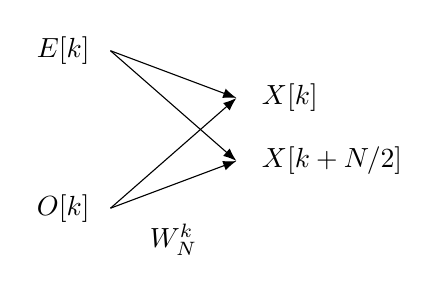
\begin{tikzpicture}[>=Latex]
\node at (0,1) {$E[k]$};
\node at (0,-1) {$O[k]$};

\draw[->] (0.6,1) -- (2.2,0.4);
\draw[->] (0.6,-1) -- (2.2,-0.4);

\draw[->] (0.6,1) -- (2.2,-0.4);
\draw[->] (0.6,-1) -- (2.2,0.4);

\node[right] at (2.4,0.4) {$X[k]$};
\node[right] at (2.4,-0.4) {$X[k+N/2]$};

\node at (1.4,-1.4) {$W_N^k$};
\end{tikzpicture}
\end{center}

The butterfly performs

\[
\boxed{
\begin{aligned}
X[k] &= E[k]+W_N^kO[k]\\
X[k+N/2] &= E[k]-W_N^kO[k]
\end{aligned}
}
\]

%%%%%%%%%%%%%%%%%%%%%%%%%%%%%%%%%%%%%%%%%%%%%%%%%%%%%%%%%%%%%%%%%%%%%%%%%%%%%%%%

\section{4-Point FFT}

Let

\[
x[n]=\{1,2,3,4\}.
\]

%%%%%%%%%%%%%%%%%%%%%%%%%%%%%%%%%%%%%%%%%%%%%%%%%%%%%%%%%%%%%%%%%%%%%%%%%%%%%%%%

\subsection{Step 1: Separate Even and Odd Samples}

Even sequence:

\[
x_e=\{1,3\}
\]

Odd sequence:

\[
x_o=\{2,4\}.
\]

%%%%%%%%%%%%%%%%%%%%%%%%%%%%%%%%%%%%%%%%%%%%%%%%%%%%%%%%%%%%%%%%%%%%%%%%%%%%%%%%

\section{2-Point DFT of Even Sequence}

For a 2-point DFT,

\[
E[0]=1+3=4
\]

\[
E[1]=1-3=-2.
\]

%%%%%%%%%%%%%%%%%%%%%%%%%%%%%%%%%%%%%%%%%%%%%%%%%%%%%%%%%%%%%%%%%%%%%%%%%%%%%%%%

\section{2-Point DFT of Odd Sequence}

\[
O[0]=2+4=6
\]

\[
O[1]=2-4=-2.
\]

%%%%%%%%%%%%%%%%%%%%%%%%%%%%%%%%%%%%%%%%%%%%%%%%%%%%%%%%%%%%%%%%%%%%%%%%%%%%%%%%

\section{Twiddle Factors}

For \(N=4\),

\[
W_4=e^{-j\pi/2}=-j.
\]

\[
W_4^0=1,
\qquad
W_4^1=-j.
\]

%%%%%%%%%%%%%%%%%%%%%%%%%%%%%%%%%%%%%%%%%%%%%%%%%%%%%%%%%%%%%%%%%%%%%%%%%%%%%%%%

\section{Combine for \(k=0\)}

\[
X[0]=E[0]+W_4^0O[0]
\]

\[
=4+6=10.
\]

\[
X[2]=E[0]-W_4^0O[0]
\]

\[
=4-6=-2.
\]

%%%%%%%%%%%%%%%%%%%%%%%%%%%%%%%%%%%%%%%%%%%%%%%%%%%%%%%%%%%%%%%%%%%%%%%%%%%%%%%%

\section{Combine for \(k=1\)}

\[
X[1]=E[1]+W_4^1O[1]
\]

\[
=-2+(-j)(-2)
=-2+2j.
\]

\[
X[3]=E[1]-W_4^1O[1]
\]

\[
=-2-2j.
\]

%%%%%%%%%%%%%%%%%%%%%%%%%%%%%%%%%%%%%%%%%%%%%%%%%%%%%%%%%%%%%%%%%%%%%%%%%%%%%%%%

\section{Final Result}

\[
\boxed{
X[k]=
\{10,\,-2+2j,\,-2,\,-2-2j\}
}
\]

%%%%%%%%%%%%%%%%%%%%%%%%%%%%%%%%%%%%%%%%%%%%%%%%%%%%%%%%%%%%%%%%%%%%%%%%%%%%%%%%

\section{Verification}

The direct DFT gives the same result, confirming the correctness of the FFT
computation.

%%%%%%%%%%%%%%%%%%%%%%%%%%%%%%%%%%%%%%%%%%%%%%%%%%%%%%%%%%%%%%%%%%%%%%%%%%%%%%%%

\section{FFT Stages}

For radix-2 FFT,

\[
\boxed{
\text{Number of stages}=\log_2N
}
\]

Examples:

\begin{table}[H]
\centering
\caption{FFT stages}
\begin{tabular}{|c|c|}
\hline
\textbf{\(N\)} & \textbf{Stages}\\
\hline
4 & 2\\
8 & 3\\
16 & 4\\
32 & 5\\
64 & 6\\
\hline
\end{tabular}
\end{table}

%%%%%%%%%%%%%%%%%%%%%%%%%%%%%%%%%%%%%%%%%%%%%%%%%%%%%%%%%%%%%%%%%%%%%%%%%%%%%%%%

\section{Butterflies per Stage}

Each stage contains

\[
\boxed{
\frac{N}{2}
}
\]

butterflies.

Total butterflies:

\[
\boxed{
\frac{N}{2}\log_2N
}
\]

%%%%%%%%%%%%%%%%%%%%%%%%%%%%%%%%%%%%%%%%%%%%%%%%%%%%%%%%%%%%%%%%%%%%%%%%%%%%%%%%

\section{Bit-Reversal Ordering}

In radix-2 DIT FFT, the input must be arranged in bit-reversed order.

%%%%%%%%%%%%%%%%%%%%%%%%%%%%%%%%%%%%%%%%%%%%%%%%%%%%%%%%%%%%%%%%%%%%%%%%%%%%%%%%

\subsection{Example for \(N=8\)}

\begin{table}[H]
\centering
\caption{Bit-reversal table}
\begin{tabular}{|c|c|c|}
\hline
\textbf{Decimal} & \textbf{Binary} & \textbf{Reversed}\\
\hline
0 & 000 & 000 (0)\\
1 & 001 & 100 (4)\\
2 & 010 & 010 (2)\\
3 & 011 & 110 (6)\\
4 & 100 & 001 (1)\\
5 & 101 & 101 (5)\\
6 & 110 & 011 (3)\\
7 & 111 & 111 (7)\\
\hline
\end{tabular}
\end{table}

The input order becomes

\[
\boxed{
\{0,4,2,6,1,5,3,7\}
}
\]

%%%%%%%%%%%%%%%%%%%%%%%%%%%%%%%%%%%%%%%%%%%%%%%%%%%%%%%%%%%%%%%%%%%%%%%%%%%%%%%%

\section{Why Bit Reversal?}

Bit reversal allows the FFT to be computed \textbf{in place}, meaning the input
array is overwritten by intermediate results and finally by the output.

This reduces memory usage significantly.

%%%%%%%%%%%%%%%%%%%%%%%%%%%%%%%%%%%%%%%%%%%%%%%%%%%%%%%%%%%%%%%%%%%%%%%%%%%%%%%%

\section{Flow Graph of 4-Point FFT}

\begin{center}
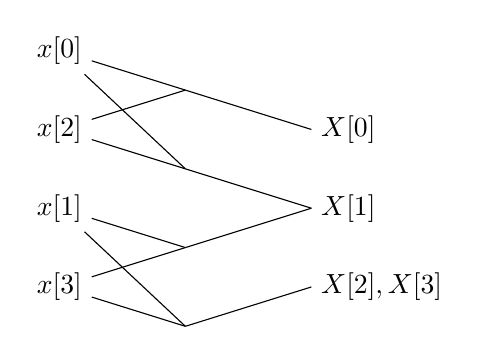
\begin{tikzpicture}[x=1.6cm,y=1cm,>=Latex]
\node (x0) at (0,3) {$x[0]$};
\node (x2) at (0,2) {$x[2]$};
\node (x1) at (0,1) {$x[1]$};
\node (x3) at (0,0) {$x[3]$};

\draw (x0) -- (1,2.5);
\draw (x2) -- (1,2.5);
\draw (x0) -- (1,1.5);
\draw (x2) -- (1,1.5);

\draw (x1) -- (1,0.5);
\draw (x3) -- (1,0.5);
\draw (x1) -- (1,-0.5);
\draw (x3) -- (1,-0.5);

\draw (1,2.5) -- (2,2);
\draw (1,1.5) -- (2,1);
\draw (1,0.5) -- (2,1);
\draw (1,-0.5) -- (2,0);

\node[right] at (2,2) {$X[0]$};
\node[right] at (2,1) {$X[1]$};
\node[right] at (2,0) {$X[2],X[3]$};
\end{tikzpicture}
\end{center}

%%%%%%%%%%%%%%%%%%%%%%%%%%%%%%%%%%%%%%%%%%%%%%%%%%%%%%%%%%%%%%%%%%%%%%%%%%%%%%%%

\section{Computational Saving}

For \(N=1024\),

Direct DFT:

\[
1024^2=1,048,576
\]

multiplications.

FFT:

\[
1024\log_2(1024)=1024\times10=10,240
\]

operations.

This is approximately

\[
\boxed{
100\times \text{ fewer operations}
}
\]

%%%%%%%%%%%%%%%%%%%%%%%%%%%%%%%%%%%%%%%%%%%%%%%%%%%%%%%%%%%%%%%%%%%%%%%%%%%%%%%%

\section{Quick Check}

\begin{enumerate}
\item \(W_4=\boxed{-j}\).
\item 8-point FFT has \(\boxed{3}\) stages.
\item Butterflies per stage for \(N=16\): \(\boxed{8}\).
\item Total butterflies for \(N=16\): \(\boxed{32}\).
\item Bit-reversal of binary \(101\) is \(\boxed{101}\) (decimal 5).
\end{enumerate}

%%%%%%%%%%%%%%%%%%%%%%%%%%%%%%%%%%%%%%%%%%%%%%%%%%%%%%%%%%%%%%%%%%%%%%%%%%%%%%%%

\begin{tcolorbox}[title=One-Minute Revision,colback=blue!5]

\[
X[k]=
\sum_{n=0}^{N-1}x[n]W_N^{kn}
\]

\[
W_N=e^{-j2\pi/N}
\]

Radix-2 DIT:

\[
X[k]=E[k]+W_N^kO[k]
\]

\[
X[k+N/2]=E[k]-W_N^kO[k]
\]

Stages:

\[
\log_2N
\]

Butterflies per stage:

\[
\frac{N}{2}
\]

Total butterflies:

\[
\frac{N}{2}\log_2N
\]

Bit-reversal is required for DIT FFT input ordering.

FFT complexity:

\[
N\log_2N
\]

\end{tcolorbox}
%%%%%%%%%%%%%%%%%%%%%%%%%%%%%%%%%%%%%%%%%%%%%%%%%%%%%%%%%%%%%%%%%%%%%%%%%%%%%%%%
%%%%%%%%%%%%%%%%%%%%%%%%%%%%%%%%%%%%%%%%%%%%%%%%%%%%%%%%%%%%%%%%%%%%%%%%%%%%%%%%
\section{Radix-2 Decimation-in-Frequency (DIF) FFT}

In the DIT algorithm, the input is divided into even and odd samples.

In the \textbf{DIF algorithm}, the frequency-domain outputs are divided into
even and odd frequency indices.

Start with

\[
X[k]=
\sum_{n=0}^{N-1}x[n]W_N^{kn}.
\]

Split the sequence into two halves:

\[
X[k]=
\sum_{n=0}^{N/2-1}x[n]W_N^{kn}
+
\sum_{n=0}^{N/2-1}x[n+N/2]W_N^{k(n+N/2)}.
\]

Using

\[
W_N^{kN/2}=(-1)^k,
\]

we obtain

\[
X[k]=
\sum_{n=0}^{N/2-1}
\left[
x[n]+(-1)^k x[n+N/2]
\right]
W_{N/2}^{kn}.
\]

%%%%%%%%%%%%%%%%%%%%%%%%%%%%%%%%%%%%%%%%%%%%%%%%%%%%%%%%%%%%%%%%%%%%%%%%%%%%%%%%

\section{DIF Butterfly Equations}

For

\[
n=0,1,\ldots,\frac{N}{2}-1,
\]

compute

\[
\boxed{
u[n]=x[n]+x[n+N/2]
}
\]

\[
\boxed{
v[n]=
\left(x[n]-x[n+N/2]\right)W_N^n
}
\]

Then perform two \((N/2)\)-point FFTs on \(u[n]\) and \(v[n]\).

%%%%%%%%%%%%%%%%%%%%%%%%%%%%%%%%%%%%%%%%%%%%%%%%%%%%%%%%%%%%%%%%%%%%%%%%%%%%%%%%

\section{DIT vs DIF}

\begin{table}[H]
\centering
\caption{DIT and DIF comparison}
\begin{tabular}{|p{4cm}|p{4cm}|p{4cm}|}
\hline
\textbf{Feature} & \textbf{DIT} & \textbf{DIF}\\
\hline
Decimation & Time & Frequency\\
\hline
Input order & Bit-reversed & Normal\\
\hline
Output order & Normal & Bit-reversed\\
\hline
Twiddle multiplication & Before butterfly output & After subtraction\\
\hline
Most common in textbooks & Yes & Yes\\
\hline
\end{tabular}
\end{table}

%%%%%%%%%%%%%%%%%%%%%%%%%%%%%%%%%%%%%%%%%%%%%%%%%%%%%%%%%%%%%%%%%%%%%%%%%%%%%%%%

\section{In-Place Computation}

FFT algorithms can overwrite the input array with intermediate results.

For example,

\[
x[0],x[1],x[2],x[3]
\]

are updated stage by stage until they contain

\[
X[0],X[1],X[2],X[3].
\]

This is called \textbf{in-place computation} and saves memory.

%%%%%%%%%%%%%%%%%%%%%%%%%%%%%%%%%%%%%%%%%%%%%%%%%%%%%%%%%%%%%%%%%%%%%%%%%%%%%%%%

\section{Inverse FFT (IFFT)}

The IDFT is

\[
x[n]=
\frac{1}{N}
\sum_{k=0}^{N-1}X[k]e^{j2\pi kn/N}.
\]

Notice that the sign in the exponent is opposite to the DFT.

%%%%%%%%%%%%%%%%%%%%%%%%%%%%%%%%%%%%%%%%%%%%%%%%%%%%%%%%%%%%%%%%%%%%%%%%%%%%%%%%

\subsection{IFFT Using FFT}

The IFFT can be computed using a forward FFT:

\[
\boxed{
x[n]=
\frac{1}{N}
\left(
\text{FFT}\{X^*[k]\}
\right)^*
}
\]

Procedure:

\begin{enumerate}
\item Take the complex conjugate of \(X[k]\).
\item Compute the FFT.
\item Take the conjugate of the result.
\item Divide by \(N\).
\end{enumerate}

%%%%%%%%%%%%%%%%%%%%%%%%%%%%%%%%%%%%%%%%%%%%%%%%%%%%%%%%%%%%%%%%%%%%%%%%%%%%%%%%

\section{Example: IFFT}

Let

\[
X[k]=\{4,0,0,0\}.
\]

Applying the IFFT,

\[
x[n]=\{1,1,1,1\}.
\]

%%%%%%%%%%%%%%%%%%%%%%%%%%%%%%%%%%%%%%%%%%%%%%%%%%%%%%%%%%%%%%%%%%%%%%%%%%%%%%%%

\section{FFT-Based Linear Convolution}

Direct convolution of long sequences is computationally expensive.

%%%%%%%%%%%%%%%%%%%%%%%%%%%%%%%%%%%%%%%%%%%%%%%%%%%%%%%%%%%%%%%%%%%%%%%%%%%%%%%%

\subsection{Procedure}

For sequences of lengths \(L_x\) and \(L_h\):

\begin{enumerate}
\item Choose
\[
N\ge L_x+L_h-1.
\]

\item Zero-pad both sequences to length \(N\).

\item Compute FFTs:
\[
X[k]=\text{FFT}\{x[n]\},
\qquad
H[k]=\text{FFT}\{h[n]\}.
\]

\item Multiply:
\[
Y[k]=X[k]H[k].
\]

\item Compute
\[
y[n]=\text{IFFT}\{Y[k]\}.
\]
\end{enumerate}

%%%%%%%%%%%%%%%%%%%%%%%%%%%%%%%%%%%%%%%%%%%%%%%%%%%%%%%%%%%%%%%%%%%%%%%%%%%%%%%%

\section{Example: FFT Convolution}

Let

\[
x[n]=\{1,2\},
\qquad
h[n]=\{1,1\}.
\]

Output length:

\[
L=2+2-1=3.
\]

Choose \(N=4\).

%%%%%%%%%%%%%%%%%%%%%%%%%%%%%%%%%%%%%%%%%%%%%%%%%%%%%%%%%%%%%%%%%%%%%%%%%%%%%%%%

\subsection{Zero-Padded Sequences}

\[
x[n]=\{1,2,0,0\},
\]

\[
h[n]=\{1,1,0,0\}.
\]

%%%%%%%%%%%%%%%%%%%%%%%%%%%%%%%%%%%%%%%%%%%%%%%%%%%%%%%%%%%%%%%%%%%%%%%%%%%%%%%%

\subsection{Result}

The IFFT gives

\[
\boxed{
y[n]=\{1,3,2,0\}.
}
\]

Ignoring the trailing zero,

\[
\boxed{
y[n]=\{1,3,2\}
}
\]

which is the correct linear convolution.

%%%%%%%%%%%%%%%%%%%%%%%%%%%%%%%%%%%%%%%%%%%%%%%%%%%%%%%%%%%%%%%%%%%%%%%%%%%%%%%%

\section{Block Convolution}

For very long signals, convolution is performed block by block.

Two standard methods are

\begin{itemize}
\item Overlap-Add (OLA),
\item Overlap-Save (OLS).
\end{itemize}

%%%%%%%%%%%%%%%%%%%%%%%%%%%%%%%%%%%%%%%%%%%%%%%%%%%%%%%%%%%%%%%%%%%%%%%%%%%%%%%%

\section{Overlap-Add Method}

%%%%%%%%%%%%%%%%%%%%%%%%%%%%%%%%%%%%%%%%%%%%%%%%%%%%%%%%%%%%%%%%%%%%%%%%%%%%%%%%

\subsection{Idea}

\begin{enumerate}
\item Divide the input into non-overlapping blocks.
\item Convolve each block with the filter using FFT.
\item Add the overlapping output portions.
\end{enumerate}

%%%%%%%%%%%%%%%%%%%%%%%%%%%%%%%%%%%%%%%%%%%%%%%%%%%%%%%%%%%%%%%%%%%%%%%%%%%%%%%%

\subsection{Block Diagram}

\begin{center}

\begin{tikzpicture}[node distance=2.2cm,>=Latex]
\node[draw,minimum width=2.4cm,minimum height=0.9cm] (blk) {Input blocks};
\node[draw,minimum width=2.6cm,minimum height=0.9cm,right of=blk] (fft) {FFT convolution};
\node[draw,minimum width=2.4cm,minimum height=0.9cm,right of=fft] (add) {Overlap \& Add};

\draw[->] (blk) -- (fft);
\draw[->] (fft) -- (add);
\end{tikzpicture}
\end{center}

%%%%%%%%%%%%%%%%%%%%%%%%%%%%%%%%%%%%%%%%%%%%%%%%%%%%%%%%%%%%%%%%%%%%%%%%%%%%%%%%

\subsection{Advantage}

Simple to understand and implement.

%%%%%%%%%%%%%%%%%%%%%%%%%%%%%%%%%%%%%%%%%%%%%%%%%%%%%%%%%%%%%%%%%%%%%%%%%%%%%%%%

\subsection{Disadvantage}

Requires addition of overlapping segments.

%%%%%%%%%%%%%%%%%%%%%%%%%%%%%%%%%%%%%%%%%%%%%%%%%%%%%%%%%%%%%%%%%%%%%%%%%%%%%%%%

\section{Overlap-Save Method}

%%%%%%%%%%%%%%%%%%%%%%%%%%%%%%%%%%%%%%%%%%%%%%%%%%%%%%%%%%%%%%%%%%%%%%%%%%%%%%%%

\subsection{Idea}

\begin{enumerate}
\item Consecutive blocks overlap by \(L_h-1\) samples.
\item Perform circular convolution using FFT.
\item Discard the corrupted samples at the beginning.
\item Keep the remaining valid samples.
\end{enumerate}

%%%%%%%%%%%%%%%%%%%%%%%%%%%%%%%%%%%%%%%%%%%%%%%%%%%%%%%%%%%%%%%%%%%%%%%%%%%%%%%%

\subsection{Advantage}

No overlap addition is required.

%%%%%%%%%%%%%%%%%%%%%%%%%%%%%%%%%%%%%%%%%%%%%%%%%%%%%%%%%%%%%%%%%%%%%%%%%%%%%%%%

\subsection{Disadvantage}

Input block management is slightly more complex.

%%%%%%%%%%%%%%%%%%%%%%%%%%%%%%%%%%%%%%%%%%%%%%%%%%%%%%%%%%%%%%%%%%%%%%%%%%%%%%%%

\section{OLA vs OLS}

\begin{table}[H]
\centering
\caption{Comparison of block convolution methods}
\begin{tabular}{|p{4cm}|p{4cm}|p{4cm}|}
\hline
\textbf{Feature} & \textbf{OLA} & \textbf{OLS}\\
\hline
Input blocks & Non-overlapping & Overlapping\\
\hline
Output processing & Add overlaps & Discard corrupted samples\\
\hline
Extra additions & Yes & No\\
\hline
Memory requirement & Moderate & Moderate\\
\hline
Practical use & Common & Very common\\
\hline
\end{tabular}
\end{table}

%%%%%%%%%%%%%%%%%%%%%%%%%%%%%%%%%%%%%%%%%%%%%%%%%%%%%%%%%%%%%%%%%%%%%%%%%%%%%%%%

\section{Computational Complexity}

For radix-2 FFT:

%%%%%%%%%%%%%%%%%%%%%%%%%%%%%%%%%%%%%%%%%%%%%%%%%%%%%%%%%%%%%%%%%%%%%%%%%%%%%%%%

\subsection{Complex Multiplications}

\[
\boxed{
\frac{N}{2}\log_2N
}
\]

%%%%%%%%%%%%%%%%%%%%%%%%%%%%%%%%%%%%%%%%%%%%%%%%%%%%%%%%%%%%%%%%%%%%%%%%%%%%%%%%

\subsection{Complex Additions}

\[
\boxed{
N\log_2N
}
\]

%%%%%%%%%%%%%%%%%%%%%%%%%%%%%%%%%%%%%%%%%%%%%%%%%%%%%%%%%%%%%%%%%%%%%%%%%%%%%%%%

\section{Example: 8-Point FFT}

\[
N=8,
\qquad
\log_2 8=3.
\]

Multiplications:

\[
\frac{8}{2}\times3=12.
\]

Additions:

\[
8\times3=24.
\]

%%%%%%%%%%%%%%%%%%%%%%%%%%%%%%%%%%%%%%%%%%%%%%%%%%%%%%%%%%%%%%%%%%%%%%%%%%%%%%%%

\section{Example: 16-Point FFT}

\[
N=16,
\qquad
\log_2 16=4.
\]

Multiplications:

\[
\frac{16}{2}\times4=32.
\]

Additions:

\[
16\times4=64.
\]

%%%%%%%%%%%%%%%%%%%%%%%%%%%%%%%%%%%%%%%%%%%%%%%%%%%%%%%%%%%%%%%%%%%%%%%%%%%%%%%%

\section{Solved Example 10.1}

How many stages are required for a 32-point radix-2 FFT?

%%%%%%%%%%%%%%%%%%%%%%%%%%%%%%%%%%%%%%%%%%%%%%%%%%%%%%%%%%%%%%%%%%%%%%%%%%%%%%%%

\subsection{Solution}

\[
\log_2 32=5.
\]

\[
\boxed{
5\text{ stages}
}
\]

%%%%%%%%%%%%%%%%%%%%%%%%%%%%%%%%%%%%%%%%%%%%%%%%%%%%%%%%%%%%%%%%%%%%%%%%%%%%%%%%

\section{Solved Example 10.2}

How many butterflies are required for a 32-point FFT?

%%%%%%%%%%%%%%%%%%%%%%%%%%%%%%%%%%%%%%%%%%%%%%%%%%%%%%%%%%%%%%%%%%%%%%%%%%%%%%%%

\subsection{Solution}

Butterflies per stage:

\[
\frac{32}{2}=16.
\]

Total butterflies:

\[
16\times5=80.
\]

\[
\boxed{
80\text{ butterflies}
}
\]

%%%%%%%%%%%%%%%%%%%%%%%%%%%%%%%%%%%%%%%%%%%%%%%%%%%%%%%%%%%%%%%%%%%%%%%%%%%%%%%%

\section{Solved Example 10.3}

Find the bit-reversed order for \(N=8\).

Using the bit-reversal table:

\[
0\rightarrow0,
\quad
1\rightarrow4,
\quad
2\rightarrow2,
\quad
3\rightarrow6,
\]

\[
4\rightarrow1,
\quad
5\rightarrow5,
\quad
6\rightarrow3,
\quad
7\rightarrow7.
\]

Hence,

\[
\boxed{
\{0,4,2,6,1,5,3,7\}
}
\]

%%%%%%%%%%%%%%%%%%%%%%%%%%%%%%%%%%%%%%%%%%%%%%%%%%%%%%%%%%%%%%%%%%%%%%%%%%%%%%%%

\section{Solved Example 10.4}

A 64-point FFT is used. Find the number of complex multiplications.

%%%%%%%%%%%%%%%%%%%%%%%%%%%%%%%%%%%%%%%%%%%%%%%%%%%%%%%%%%%%%%%%%%%%%%%%%%%%%%%%

\subsection{Solution}

\[
\frac{64}{2}\log_2 64
=
32\times6
=
192.
\]

\[
\boxed{
192
}
\]

%%%%%%%%%%%%%%%%%%%%%%%%%%%%%%%%%%%%%%%%%%%%%%%%%%%%%%%%%%%%%%%%%%%%%%%%%%%%%%%%

\section{Solved Example 10.5}

A sequence of length 100 is convolved with a filter of length 25 using FFT.

Minimum FFT size:

\[
N\ge100+25-1=124.
\]

Choose the next power of two:

\[
\boxed{
N=128
}
\]

%%%%%%%%%%%%%%%%%%%%%%%%%%%%%%%%%%%%%%%%%%%%%%%%%%%%%%%%%%%%%%%%%%%%%%%%%%%%%%%%

\section{Important GATE Points}

\begin{enumerate}
\item FFT is an algorithm, not a new transform.
\item Radix-2 FFT requires \(N=2^m\).
\item DIT: bit-reversed input, normal output.
\item DIF: normal input, bit-reversed output.
\item IFFT can be computed using FFT and conjugation.
\item FFT-based convolution requires zero padding.
\item OLA adds overlaps; OLS discards corrupted samples.
\item Complexity is \(N\log_2N\), not \(N^2\).
\end{enumerate}

%%%%%%%%%%%%%%%%%%%%%%%%%%%%%%%%%%%%%%%%%%%%%%%%%%%%%%%%%%%%%%%%%%%%%%%%%%%%%%%%

\section{Chapter Summary}

In this chapter, we derived the radix-2 DIT FFT and introduced the DIF FFT,
butterfly operations, bit-reversal ordering and in-place computation.

We also studied the IFFT, FFT-based linear convolution and the practical block
convolution methods OLA and OLS.

These techniques are used in spectrum analyzers, communication systems, audio
processing, radar, image processing and real-time embedded DSP systems.

%%%%%%%%%%%%%%%%%%%%%%%%%%%%%%%%%%%%%%%%%%%%%%%%%%%%%%%%%%%%%%%%%%%%%%%%%%%%%%%%

\begin{tcolorbox}[title=One-Minute Revision,colback=blue!5]

FFT complexity:

\[
N\log_2N
\]

DIT butterfly:

\[
X[k]=E[k]+W_N^kO[k]
\]

\[
X[k+N/2]=E[k]-W_N^kO[k]
\]

DIF butterfly:

\[
u[n]=x[n]+x[n+N/2]
\]

\[
v[n]=(x[n]-x[n+N/2])W_N^n
\]

Stages:

\[
\log_2N
\]

Butterflies:

\[
\frac{N}{2}\log_2N
\]

IFFT:

\[
x[n]=
\frac{1}{N}
\left(
\text{FFT}\{X^*[k]\}
\right)^*
\]

Linear convolution:

\[
N\ge L_x+L_h-1
\]

OLA: add overlaps.

OLS: discard corrupted samples.

\end{tcolorbox}
%%%%%%%%%%%%%%%%%%%%%%%%%%%%%%%%%%%%%%%%%%%%%%%%%%%%%%%%%%%%%%%%%%%%%%%%%%%%%%%%
%%%%%%%%%%%%%%%%%%%%%%%%%%%%%%%%%%%%%%%%%%%%%%%%%%%%%%%%%%%%%%%%%%%%%%%%%%%%%%%%
% CHAPTER 11
%%%%%%%%%%%%%%%%%%%%%%%%%%%%%%%%%%%%%%%%%%%%%%%%%%%%%%%%%%%%%%%%%%%%%%%%%%%%%%%%

\chapter{z-Transform}

\begin{tcolorbox}[colback=blue!5!white,colframe=blue!70!black,title=Learning Objectives]

After studying this chapter, the reader will be able to

\begin{itemize}
\item Understand the need for the z-transform.
\item Define the bilateral and unilateral z-transforms.
\item Determine the Region of Convergence (ROC).
\item Compute z-transforms of standard sequences.
\item Understand poles and zeros.
\item Relate the z-transform to the DTFT.
\end{itemize}

\end{tcolorbox}

%%%%%%%%%%%%%%%%%%%%%%%%%%%%%%%%%%%%%%%%%%%%%%%%%%%%%%%%%%%%%%%%%%%%%%%%%%%%%%%%

\section{Introduction}

The DTFT is useful for frequency analysis, but it does not exist for many important
sequences.

Example:

\[
x[n]=u[n]
\]

has a DTFT that is not absolutely convergent.

To analyze such sequences and solve difference equations systematically, we use the
\textbf{z-transform}.

The z-transform is the discrete-time counterpart of the Laplace transform.

%%%%%%%%%%%%%%%%%%%%%%%%%%%%%%%%%%%%%%%%%%%%%%%%%%%%%%%%%%%%%%%%%%%%%%%%%%%%%%%%

\section{Complex Variable \(z\)}

The complex variable is written as

\[
\boxed{
z=re^{j\omega}
}
\]

where

\begin{itemize}
\item \(r\): magnitude,
\item \(\omega\): angle.
\end{itemize}

The \(z\)-plane is a complex plane with

\[
z=\sigma+j\Omega.
\]

The unit circle is

\[
\boxed{
|z|=1.
}
\]

%%%%%%%%%%%%%%%%%%%%%%%%%%%%%%%%%%%%%%%%%%%%%%%%%%%%%%%%%%%%%%%%%%%%%%%%%%%%%%%%

\section{Bilateral z-Transform}

The bilateral (two-sided) z-transform is

\[
\boxed{
X(z)=
\sum_{n=-\infty}^{\infty}
x[n]z^{-n}
}
\]

The summation includes all integer values of \(n\).

%%%%%%%%%%%%%%%%%%%%%%%%%%%%%%%%%%%%%%%%%%%%%%%%%%%%%%%%%%%%%%%%%%%%%%%%%%%%%%%%

\section{Region of Convergence (ROC)}

The values of \(z\) for which the series converges form the
\textbf{Region of Convergence}.

\[
\boxed{
\text{ROC}=
\{z:\sum |x[n]z^{-n}|<\infty\}
}
\]

The ROC is as important as the transform itself.

%%%%%%%%%%%%%%%%%%%%%%%%%%%%%%%%%%%%%%%%%%%%%%%%%%%%%%%%%%%%%%%%%%%%%%%%%%%%%%%%

\section{Unilateral z-Transform}

For causal sequences, we often use the one-sided transform:

\[
\boxed{
X^+(z)=
\sum_{n=0}^{\infty}
x[n]z^{-n}
}
\]

This is convenient for solving difference equations with initial conditions.

%%%%%%%%%%%%%%%%%%%%%%%%%%%%%%%%%%%%%%%%%%%%%%%%%%%%%%%%%%%%%%%%%%%%%%%%%%%%%%%%

\section{z-Transform of the Unit Sample}

Let

\[
x[n]=\delta[n].
\]

Then

\[
X(z)=
\sum_{n=-\infty}^{\infty}
\delta[n]z^{-n}.
\]

Only \(n=0\) contributes:

\[
\boxed{
X(z)=1
}
\]

The ROC is the entire \(z\)-plane.

%%%%%%%%%%%%%%%%%%%%%%%%%%%%%%%%%%%%%%%%%%%%%%%%%%%%%%%%%%%%%%%%%%%%%%%%%%%%%%%%

\section{z-Transform of the Unit Step}

Let

\[
x[n]=u[n].
\]

Then

\[
X(z)=
\sum_{n=0}^{\infty}z^{-n}.
\]

This is a geometric series:

\[
X(z)=
\frac{1}{1-z^{-1}}
\]

provided

\[
|z^{-1}|<1.
\]

Hence,

\[
\boxed{
u[n]
\xleftrightarrow{\mathcal{Z}}
\frac{1}{1-z^{-1}},
\qquad
\text{ROC: }|z|>1
}
\]

%%%%%%%%%%%%%%%%%%%%%%%%%%%%%%%%%%%%%%%%%%%%%%%%%%%%%%%%%%%%%%%%%%%%%%%%%%%%%%%%

\section{z-Transform of \(a^n u[n]\)}

Let

\[
x[n]=a^n u[n].
\]

Then

\[
X(z)=
\sum_{n=0}^{\infty}
a^n z^{-n}
=
\sum_{n=0}^{\infty}
(az^{-1})^n.
\]

Therefore,

\[
\boxed{
X(z)=
\frac{1}{1-az^{-1}},
\qquad
\text{ROC: }|z|>|a|
}
\]

%%%%%%%%%%%%%%%%%%%%%%%%%%%%%%%%%%%%%%%%%%%%%%%%%%%%%%%%%%%%%%%%%%%%%%%%%%%%%%%%

\section{Example}

For

\[
x[n]=\left(\frac12\right)^n u[n],
\]

\[
\boxed{
X(z)=
\frac{1}{1-\frac12 z^{-1}},
\qquad
\text{ROC: }|z|>\frac12
}
\]

%%%%%%%%%%%%%%%%%%%%%%%%%%%%%%%%%%%%%%%%%%%%%%%%%%%%%%%%%%%%%%%%%%%%%%%%%%%%%%%%

\section{Left-Sided Sequence}

Consider

\[
x[n]=-a^n u[-n-1].
\]

Then

\[
X(z)=
\sum_{n=-\infty}^{-1}
(-a^n)z^{-n}.
\]

After simplification,

\[
\boxed{
X(z)=
\frac{1}{1-az^{-1}},
\qquad
\text{ROC: }|z|<|a|
}
\]

Notice that the algebraic expression is the same as the right-sided sequence, but
the ROC is different.

%%%%%%%%%%%%%%%%%%%%%%%%%%%%%%%%%%%%%%%%%%%%%%%%%%%%%%%%%%%%%%%%%%%%%%%%%%%%%%%%

\section{ROC Determines the Sequence}

\[
\frac{1}{1-az^{-1}}
\]

can represent three different sequences:

\begin{table}[H]
\centering
\caption{Same transform, different ROCs}
\begin{tabular}{|p{5cm}|p{5cm}|}
\hline
\textbf{Sequence} & \textbf{ROC}\\
\hline
\(a^n u[n]\) & \(|z|>|a|\)\\
\hline
\(-a^n u[-n-1]\) & \(|z|<|a|\)\\
\hline
No two-sided sequence exists & \(|z|=|a|\)\\
\hline
\end{tabular}
\end{table}

%%%%%%%%%%%%%%%%%%%%%%%%%%%%%%%%%%%%%%%%%%%%%%%%%%%%%%%%%%%%%%%%%%%%%%%%%%%%%%%%

\section{Poles and Zeros}

%%%%%%%%%%%%%%%%%%%%%%%%%%%%%%%%%%%%%%%%%%%%%%%%%%%%%%%%%%%%%%%%%%%%%%%%%%%%%%%%

\subsection{Zero}

A value of \(z\) that makes

\[
X(z)=0.
\]

%%%%%%%%%%%%%%%%%%%%%%%%%%%%%%%%%%%%%%%%%%%%%%%%%%%%%%%%%%%%%%%%%%%%%%%%%%%%%%%%

\subsection{Pole}

A value of \(z\) that makes

\[
X(z)\to\infty.
\]

%%%%%%%%%%%%%%%%%%%%%%%%%%%%%%%%%%%%%%%%%%%%%%%%%%%%%%%%%%%%%%%%%%%%%%%%%%%%%%%%

\subsection{Example}

\[
X(z)=
\frac{1-z^{-1}}
{1-0.5z^{-1}}.
\]

Zero:

\[
z=1.
\]

Pole:

\[
z=0.5.
\]

%%%%%%%%%%%%%%%%%%%%%%%%%%%%%%%%%%%%%%%%%%%%%%%%%%%%%%%%%%%%%%%%%%%%%%%%%%%%%%%%

\section{Pole-Zero Plot}

\begin{center}
\begin{tikzpicture}[scale=2]
\draw[->] (-1.5,0) -- (1.5,0) node[right] {Re};
\draw[->] (0,-1.2) -- (0,1.2) node[above] {Im};

\draw (0,0) circle (1);

\draw[thick] (1,0) node[circle,draw,inner sep=1.5pt] {};
\draw[thick] (0.5,0) node[cross out,draw,inner sep=2pt] {};

\node[below] at (1,0) {$z=1$};
\node[below] at (0.5,0) {$z=0.5$};
\end{tikzpicture}
\end{center}

Convention:

\begin{itemize}
\item \(\circ\): zero,
\item \(\times\): pole.
\end{itemize}

%%%%%%%%%%%%%%%%%%%%%%%%%%%%%%%%%%%%%%%%%%%%%%%%%%%%%%%%%%%%%%%%%%%%%%%%%%%%%%%%

\section{ROC of Rational Functions}

For rational functions, the ROC is an annular region.

%%%%%%%%%%%%%%%%%%%%%%%%%%%%%%%%%%%%%%%%%%%%%%%%%%%%%%%%%%%%%%%%%%%%%%%%%%%%%%%%

\subsection{Example}

\[
X(z)=
\frac{1}
{(1-0.5z^{-1})(1-2z^{-1})}.
\]

Possible ROCs:

\begin{itemize}
\item \(|z|>2\),
\item \(0.5<|z|<2\),
\item \(|z|<0.5\).
\end{itemize}

The ROC cannot contain poles.

%%%%%%%%%%%%%%%%%%%%%%%%%%%%%%%%%%%%%%%%%%%%%%%%%%%%%%%%%%%%%%%%%%%%%%%%%%%%%%%%

\section{Causality from ROC}

A rational sequence is causal if

\[
\boxed{
\text{ROC is outside the outermost pole.}
}
\]

Example:

\[
X(z)=
\frac{1}{1-0.5z^{-1}},
\qquad
\text{ROC: }|z|>0.5.
\]

This corresponds to

\[
x[n]=(0.5)^n u[n]
\]

which is causal.

%%%%%%%%%%%%%%%%%%%%%%%%%%%%%%%%%%%%%%%%%%%%%%%%%%%%%%%%%%%%%%%%%%%%%%%%%%%%%%%%

\section{Stability from ROC}

A sequence is stable if the DTFT exists, which requires the ROC to include the unit circle.

\[
\boxed{
|z|=1 \in \text{ROC}
}
\]

For the previous example,

\[
|z|>0.5
\]

includes \(|z|=1\), so the sequence is stable.

%%%%%%%%%%%%%%%%%%%%%%%%%%%%%%%%%%%%%%%%%%%%%%%%%%%%%%%%%%%%%%%%%%%%%%%%%%%%%%%%

\section{Connection with DTFT}

Evaluate the z-transform on the unit circle:

\[
\boxed{
X(e^{j\omega})=
X(z)\Big|_{z=e^{j\omega}}
}
\]

This is valid only if the unit circle lies inside the ROC.

%%%%%%%%%%%%%%%%%%%%%%%%%%%%%%%%%%%%%%%%%%%%%%%%%%%%%%%%%%%%%%%%%%%%%%%%%%%%%%%%

\section{Example}

\[
X(z)=
\frac{1}{1-0.5z^{-1}},
\qquad
|z|>0.5.
\]

Since the unit circle is included,

\[
X(e^{j\omega})=
\frac{1}{1-0.5e^{-j\omega}}.
\]

This is exactly the DTFT of \((0.5)^n u[n]\).

%%%%%%%%%%%%%%%%%%%%%%%%%%%%%%%%%%%%%%%%%%%%%%%%%%%%%%%%%%%%%%%%%%%%%%%%%%%%%%%%

\section{Initial Value Theorem}

For causal sequences,

\[
\boxed{
x[0]=
\lim_{z\to\infty}X(z)
}
\]

%%%%%%%%%%%%%%%%%%%%%%%%%%%%%%%%%%%%%%%%%%%%%%%%%%%%%%%%%%%%%%%%%%%%%%%%%%%%%%%%

\subsection{Example}

\[
X(z)=
\frac{1}{1-0.5z^{-1}}.
\]

Then

\[
x[0]=
\lim_{z\to\infty}
\frac{1}{1-0.5z^{-1}}
=1.
\]

%%%%%%%%%%%%%%%%%%%%%%%%%%%%%%%%%%%%%%%%%%%%%%%%%%%%%%%%%%%%%%%%%%%%%%%%%%%%%%%%

\section{Final Value Theorem}

If the limits exist and all poles of \((1-z^{-1})X(z)\) are inside the unit circle,

\[
\boxed{
\lim_{n\to\infty}x[n]
=
\lim_{z\to1}(1-z^{-1})X(z)
}
\]

%%%%%%%%%%%%%%%%%%%%%%%%%%%%%%%%%%%%%%%%%%%%%%%%%%%%%%%%%%%%%%%%%%%%%%%%%%%%%%%%

\subsection{Example}

\[
X(z)=
\frac{1}{1-0.5z^{-1}}.
\]

\[
(1-z^{-1})X(z)=
\frac{1-z^{-1}}{1-0.5z^{-1}}.
\]

At \(z=1\),

\[
\lim_{n\to\infty}x[n]=0.
\]

This matches

\[
(0.5)^n\to0.
\]

%%%%%%%%%%%%%%%%%%%%%%%%%%%%%%%%%%%%%%%%%%%%%%%%%%%%%%%%%%%%%%%%%%%%%%%%%%%%%%%%

\section{Common ROC Patterns}

\begin{table}[H]
\centering
\caption{ROC patterns}
\begin{tabular}{|p{4cm}|p{5cm}|}
\hline
\textbf{Sequence Type} & \textbf{ROC}\\
\hline
Right-sided & Outside outermost pole\\
\hline
Left-sided & Inside innermost pole\\
\hline
Two-sided & Between poles\\
\hline
Finite-duration right-sided & Entire plane except \(z=0\)\\
\hline
Finite-duration left-sided & Entire plane except \(z=\infty\)\\
\hline
\end{tabular}
\end{table}

%%%%%%%%%%%%%%%%%%%%%%%%%%%%%%%%%%%%%%%%%%%%%%%%%%%%%%%%%%%%%%%%%%%%%%%%%%%%%%%%

\section{Solved Example 11.1}

Find the z-transform of

\[
x[n]=3^n u[n].
\]

%%%%%%%%%%%%%%%%%%%%%%%%%%%%%%%%%%%%%%%%%%%%%%%%%%%%%%%%%%%%%%%%%%%%%%%%%%%%%%%%

\subsection{Solution}

\[
X(z)=
\sum_{n=0}^{\infty}(3z^{-1})^n
=
\frac{1}{1-3z^{-1}}
\]

with ROC

\[
\boxed{
|z|>3
}
\]

%%%%%%%%%%%%%%%%%%%%%%%%%%%%%%%%%%%%%%%%%%%%%%%%%%%%%%%%%%%%%%%%%%%%%%%%%%%%%%%%

\section{Solved Example 11.2}

Find the z-transform of

\[
x[n]=-\left(\frac12\right)^n u[-n-1].
\]

%%%%%%%%%%%%%%%%%%%%%%%%%%%%%%%%%%%%%%%%%%%%%%%%%%%%%%%%%%%%%%%%%%%%%%%%%%%%%%%%

\subsection{Solution}

\[
\boxed{
X(z)=
\frac{1}{1-\frac12 z^{-1}},
\qquad
\text{ROC: }|z|<\frac12
}
\]

%%%%%%%%%%%%%%%%%%%%%%%%%%%%%%%%%%%%%%%%%%%%%%%%%%%%%%%%%%%%%%%%%%%%%%%%%%%%%%%%

\section{Solved Example 11.3}

Determine whether the sequence is stable:

\[
X(z)=
\frac{1}{1-2z^{-1}},
\qquad
\text{ROC: }|z|>2.
\]

%%%%%%%%%%%%%%%%%%%%%%%%%%%%%%%%%%%%%%%%%%%%%%%%%%%%%%%%%%%%%%%%%%%%%%%%%%%%%%%%

\subsection{Solution}

The unit circle \(|z|=1\) is not included in the ROC.

Hence,

\[
\boxed{
\text{The sequence is unstable.}
}
\]

%%%%%%%%%%%%%%%%%%%%%%%%%%%%%%%%%%%%%%%%%%%%%%%%%%%%%%%%%%%%%%%%%%%%%%%%%%%%%%%%

\section{Solved Example 11.4}

Find the poles and zeros of

\[
X(z)=
\frac{1-z^{-1}}
{1-0.25z^{-1}}.
\]

%%%%%%%%%%%%%%%%%%%%%%%%%%%%%%%%%%%%%%%%%%%%%%%%%%%%%%%%%%%%%%%%%%%%%%%%%%%%%%%%

\subsection{Solution}

Zero:

\[
\boxed{
z=1
}
\]

Pole:

\[
\boxed{
z=0.25
}
\]

%%%%%%%%%%%%%%%%%%%%%%%%%%%%%%%%%%%%%%%%%%%%%%%%%%%%%%%%%%%%%%%%%%%%%%%%%%%%%%%%

\section{Quick Check}

\begin{enumerate}
\item \(u[n]\rightarrow \boxed{\dfrac{1}{1-z^{-1}}}\).
\item ROC of \(u[n]\): \(\boxed{|z|>1}\).
\item Pole of \(\dfrac{1}{1-0.5z^{-1}}\): \(\boxed{0.5}\).
\item Stable if: \(\boxed{\text{unit circle is in ROC}}\).
\item DTFT is obtained by: \(\boxed{z=e^{j\omega}}\).
\end{enumerate}

%%%%%%%%%%%%%%%%%%%%%%%%%%%%%%%%%%%%%%%%%%%%%%%%%%%%%%%%%%%%%%%%%%%%%%%%%%%%%%%%

\begin{tcolorbox}[title=One-Minute Revision,colback=blue!5]

\[
X(z)=
\sum_{n=-\infty}^{\infty}x[n]z^{-n}
\]

\[
X^+(z)=
\sum_{n=0}^{\infty}x[n]z^{-n}
\]

\[
u[n]\leftrightarrow
\frac{1}{1-z^{-1}},
\quad |z|>1
\]

\[
a^n u[n]\leftrightarrow
\frac{1}{1-az^{-1}},
\quad |z|>|a|
\]

Pole: denominator zero.

Zero: numerator zero.

Causal:

\[
\text{ROC outside outermost pole}
\]

Stable:

\[
|z|=1 \in \text{ROC}
\]

DTFT:

\[
X(e^{j\omega})=X(z)|_{z=e^{j\omega}}
\]

\end{tcolorbox}
%%%%%%%%%%%%%%%%%%%%%%%%%%%%%%%%%%%%%%%%%%%%%%%%%%%%%%%%%%%%%%%%%%%%%%%%%%%%%%%%
%%%%%%%%%%%%%%%%%%%%%%%%%%%%%%%%%%%%%%%%%%%%%%%%%%%%%%%%%%%%%%%%%%%%%%%%%%%%%%%%
\section{Linearity Property}

If

\[
x_1[n]\xleftrightarrow{\mathcal{Z}}X_1(z)
\]

and

\[
x_2[n]\xleftrightarrow{\mathcal{Z}}X_2(z),
\]

then

\[
\boxed{
a_1x_1[n]+a_2x_2[n]
\xleftrightarrow{\mathcal{Z}}
a_1X_1(z)+a_2X_2(z)
}
\]

%%%%%%%%%%%%%%%%%%%%%%%%%%%%%%%%%%%%%%%%%%%%%%%%%%%%%%%%%%%%%%%%%%%%%%%%%%%%%%%%

\section{Time-Shifting Property}

%%%%%%%%%%%%%%%%%%%%%%%%%%%%%%%%%%%%%%%%%%%%%%%%%%%%%%%%%%%%%%%%%%%%%%%%%%%%%%%%

\subsection{Delay}

\[
\boxed{
x[n-n_0]
\xleftrightarrow{\mathcal{Z}}
z^{-n_0}X(z)
}
\]

For bilateral transforms, the ROC is unchanged except possibly at the origin or infinity.

%%%%%%%%%%%%%%%%%%%%%%%%%%%%%%%%%%%%%%%%%%%%%%%%%%%%%%%%%%%%%%%%%%%%%%%%%%%%%%%%

\subsection{Advance}

\[
\boxed{
x[n+n_0]
\xleftrightarrow{\mathcal{Z}}
z^{n_0}X(z)
}
\]

with additional terms for unilateral transforms.

%%%%%%%%%%%%%%%%%%%%%%%%%%%%%%%%%%%%%%%%%%%%%%%%%%%%%%%%%%%%%%%%%%%%%%%%%%%%%%%%

\section{Scaling Property}

\[
\boxed{
a^n x[n]
\xleftrightarrow{\mathcal{Z}}
X\left(\frac{z}{a}\right)
}
\]

%%%%%%%%%%%%%%%%%%%%%%%%%%%%%%%%%%%%%%%%%%%%%%%%%%%%%%%%%%%%%%%%%%%%%%%%%%%%%%%%

\section{Time Reversal}

\[
\boxed{
x[-n]
\xleftrightarrow{\mathcal{Z}}
X(z^{-1})
}
\]

The ROC is inverted with respect to the unit circle.

%%%%%%%%%%%%%%%%%%%%%%%%%%%%%%%%%%%%%%%%%%%%%%%%%%%%%%%%%%%%%%%%%%%%%%%%%%%%%%%%

\section{Convolution Property}

If

\[
y[n]=x[n]*h[n],
\]

then

\[
\boxed{
Y(z)=X(z)H(z)
}
\]

This is one of the most powerful properties of the z-transform.

%%%%%%%%%%%%%%%%%%%%%%%%%%%%%%%%%%%%%%%%%%%%%%%%%%%%%%%%%%%%%%%%%%%%%%%%%%%%%%%%

\section{Differentiation Property}

\[
\boxed{
nx[n]
\xleftrightarrow{\mathcal{Z}}
-z\frac{dX(z)}{dz}
}
\]

This is useful for finding moments of sequences.

%%%%%%%%%%%%%%%%%%%%%%%%%%%%%%%%%%%%%%%%%%%%%%%%%%%%%%%%%%%%%%%%%%%%%%%%%%%%%%%%

\section{Initial Value Theorem}

For causal sequences,

\[
\boxed{
x[0]=\lim_{z\to\infty}X(z)
}
\]

%%%%%%%%%%%%%%%%%%%%%%%%%%%%%%%%%%%%%%%%%%%%%%%%%%%%%%%%%%%%%%%%%%%%%%%%%%%%%%%%

\subsection{Example}

\[
X(z)=
\frac{1}{1-0.5z^{-1}}.
\]

Then

\[
x[0]=
\lim_{z\to\infty}
\frac{1}{1-0.5z^{-1}}
=1.
\]

%%%%%%%%%%%%%%%%%%%%%%%%%%%%%%%%%%%%%%%%%%%%%%%%%%%%%%%%%%%%%%%%%%%%%%%%%%%%%%%%

\section{Final Value Theorem}

If all poles of \((1-z^{-1})X(z)\) are inside the unit circle,

\[
\boxed{
\lim_{n\to\infty}x[n]
=
\lim_{z\to1}(1-z^{-1})X(z)
}
\]

%%%%%%%%%%%%%%%%%%%%%%%%%%%%%%%%%%%%%%%%%%%%%%%%%%%%%%%%%%%%%%%%%%%%%%%%%%%%%%%%

\subsection{Example}

\[
X(z)=
\frac{1}{1-0.5z^{-1}}.
\]

\[
(1-z^{-1})X(z)=
\frac{1-z^{-1}}{1-0.5z^{-1}}.
\]

At \(z=1\),

\[
\lim_{n\to\infty}x[n]=0.
\]

%%%%%%%%%%%%%%%%%%%%%%%%%%%%%%%%%%%%%%%%%%%%%%%%%%%%%%%%%%%%%%%%%%%%%%%%%%%%%%%%

\section{Inverse z-Transform}

We now recover \(x[n]\) from \(X(z)\).

%%%%%%%%%%%%%%%%%%%%%%%%%%%%%%%%%%%%%%%%%%%%%%%%%%%%%%%%%%%%%%%%%%%%%%%%%%%%%%%%

\subsection{Method 1: Power-Series Expansion}

Given

\[
X(z)=
\frac{1}{1-0.5z^{-1}},
\qquad |z|>0.5,
\]

expand as

\[
X(z)=
1+0.5z^{-1}+0.25z^{-2}+\cdots
\]

Hence,

\[
\boxed{
x[n]=(0.5)^n u[n]
}
\]

%%%%%%%%%%%%%%%%%%%%%%%%%%%%%%%%%%%%%%%%%%%%%%%%%%%%%%%%%%%%%%%%%%%%%%%%%%%%%%%%

\section{Method 2: Partial-Fraction Expansion}

Consider

\[
X(z)=
\frac{1}
{(1-0.5z^{-1})(1-0.25z^{-1})}.
\]

Assume

\[
X(z)=
\frac{A}{1-0.5z^{-1}}
+
\frac{B}{1-0.25z^{-1}}.
\]

%%%%%%%%%%%%%%%%%%%%%%%%%%%%%%%%%%%%%%%%%%%%%%%%%%%%%%%%%%%%%%%%%%%%%%%%%%%%%%%%

\subsection{Find \(A\) and \(B\)}

Multiplying both sides,

\[
1=A(1-0.25z^{-1})+B(1-0.5z^{-1}).
\]

Set

\[
z^{-1}=2
\]

to eliminate the first denominator:

\[
1=B(1-1)=0
\]

Instead, compare coefficients:

\[
A+B=1
\]

\[
0.25A+0.5B=0.
\]

Solving,

\[
A=2,
\qquad
B=-1.
\]

%%%%%%%%%%%%%%%%%%%%%%%%%%%%%%%%%%%%%%%%%%%%%%%%%%%%%%%%%%%%%%%%%%%%%%%%%%%%%%%%

\subsection{Inverse Transform}

\[
\boxed{
x[n]=
2(0.5)^n u[n]
-(0.25)^n u[n]
}
\]

%%%%%%%%%%%%%%%%%%%%%%%%%%%%%%%%%%%%%%%%%%%%%%%%%%%%%%%%%%%%%%%%%%%%%%%%%%%%%%%%

\section{Repeated Poles}

If

\[
X(z)=
\frac{1}{(1-az^{-1})^2},
\]

then

\[
\boxed{
x[n]=(n+1)a^n u[n]
}
\]

Repeated poles produce polynomial factors in time.

%%%%%%%%%%%%%%%%%%%%%%%%%%%%%%%%%%%%%%%%%%%%%%%%%%%%%%%%%%%%%%%%%%%%%%%%%%%%%%%%

\section{Difference Equations}

Consider the first-order equation

\[
y[n]-0.5y[n-1]=x[n].
\]

%%%%%%%%%%%%%%%%%%%%%%%%%%%%%%%%%%%%%%%%%%%%%%%%%%%%%%%%%%%%%%%%%%%%%%%%%%%%%%%%

\subsection{Zero Initial Conditions}

Taking the unilateral z-transform,

\[
Y(z)-0.5z^{-1}Y(z)=X(z).
\]

Hence,

\[
Y(z)=
\frac{X(z)}{1-0.5z^{-1}}.
\]

Therefore,

\[
\boxed{
H(z)=
\frac{1}{1-0.5z^{-1}}
}
\]

%%%%%%%%%%%%%%%%%%%%%%%%%%%%%%%%%%%%%%%%%%%%%%%%%%%%%%%%%%%%%%%%%%%%%%%%%%%%%%%%

\section{Impulse Response}

For

\[
x[n]=\delta[n],
\]

\[
X(z)=1.
\]

Thus,

\[
H(z)=
\frac{1}{1-0.5z^{-1}}.
\]

Inverse transform:

\[
\boxed{
h[n]=(0.5)^n u[n]
}
\]

%%%%%%%%%%%%%%%%%%%%%%%%%%%%%%%%%%%%%%%%%%%%%%%%%%%%%%%%%%%%%%%%%%%%%%%%%%%%%%%%

\section{Step Response}

For

\[
x[n]=u[n],
\]

\[
X(z)=
\frac{1}{1-z^{-1}}.
\]

Then

\[
Y(z)=
\frac{1}{(1-z^{-1})(1-0.5z^{-1})}.
\]

Using partial fractions,

\[
Y(z)=
\frac{2}{1-z^{-1}}
-
\frac{1}{1-0.5z^{-1}}.
\]

Hence,

\[
\boxed{
y[n]=
2u[n]-(0.5)^n u[n]
}
\]

%%%%%%%%%%%%%%%%%%%%%%%%%%%%%%%%%%%%%%%%%%%%%%%%%%%%%%%%%%%%%%%%%%%%%%%%%%%%%%%%

\section{System Function}

For a general difference equation

\[
\sum_{k=0}^{N}a_k y[n-k]
=
\sum_{k=0}^{M}b_k x[n-k],
\]

taking the z-transform gives

\[
H(z)=
\frac{Y(z)}{X(z)}
=
\frac{\sum_{k=0}^{M}b_k z^{-k}}
{\sum_{k=0}^{N}a_k z^{-k}}.
\]

%%%%%%%%%%%%%%%%%%%%%%%%%%%%%%%%%%%%%%%%%%%%%%%%%%%%%%%%%%%%%%%%%%%%%%%%%%%%%%%%

\section{Pole-Zero Interpretation}

%%%%%%%%%%%%%%%%%%%%%%%%%%%%%%%%%%%%%%%%%%%%%%%%%%%%%%%%%%%%%%%%%%%%%%%%%%%%%%%%

\subsection{Poles Near the Unit Circle}

\begin{itemize}
\item Produce sharp resonances.
\item Give long impulse responses.
\item Make the system more selective.
\end{itemize}

%%%%%%%%%%%%%%%%%%%%%%%%%%%%%%%%%%%%%%%%%%%%%%%%%%%%%%%%%%%%%%%%%%%%%%%%%%%%%%%%

\subsection{Zeros on the Unit Circle}

\begin{itemize}
\item Create frequency nulls.
\item Completely reject specific frequencies.
\end{itemize}

%%%%%%%%%%%%%%%%%%%%%%%%%%%%%%%%%%%%%%%%%%%%%%%%%%%%%%%%%%%%%%%%%%%%%%%%%%%%%%%%

\section{Example: Notch Filter}

\[
H(z)=
\frac{1-2\cos\omega_0 z^{-1}+z^{-2}}
{1-r(2\cos\omega_0)z^{-1}+r^2 z^{-2}}.
\]

Zeros at

\[
z=e^{\pm j\omega_0}
\]

create a notch at frequency \(\omega_0\).

%%%%%%%%%%%%%%%%%%%%%%%%%%%%%%%%%%%%%%%%%%%%%%%%%%%%%%%%%%%%%%%%%%%%%%%%%%%%%%%%

\section{Stability Criterion}

A causal rational system is stable if all poles lie strictly inside the unit circle:

\[
\boxed{
|p_i|<1
}
\]

%%%%%%%%%%%%%%%%%%%%%%%%%%%%%%%%%%%%%%%%%%%%%%%%%%%%%%%%%%%%%%%%%%%%%%%%%%%%%%%%

\section{Example}

\[
H(z)=
\frac{1}{1-1.2z^{-1}}.
\]

Pole:

\[
z=1.2.
\]

Since

\[
|1.2|>1,
\]

\[
\boxed{
\text{The system is unstable.}
}
\]

%%%%%%%%%%%%%%%%%%%%%%%%%%%%%%%%%%%%%%%%%%%%%%%%%%%%%%%%%%%%%%%%%%%%%%%%%%%%%%%%

\section{Solved Example 11.5}

Find the inverse z-transform of

\[
X(z)=
\frac{1}{1-0.8z^{-1}},
\qquad |z|>0.8.
\]

%%%%%%%%%%%%%%%%%%%%%%%%%%%%%%%%%%%%%%%%%%%%%%%%%%%%%%%%%%%%%%%%%%%%%%%%%%%%%%%%

\subsection{Solution}

Using the standard pair,

\[
\boxed{
x[n]=(0.8)^n u[n]
}
\]

%%%%%%%%%%%%%%%%%%%%%%%%%%%%%%%%%%%%%%%%%%%%%%%%%%%%%%%%%%%%%%%%%%%%%%%%%%%%%%%%

\section{Solved Example 11.6}

Find the inverse z-transform of

\[
X(z)=
\frac{1}{1-0.8z^{-1}},
\qquad |z|<0.8.
\]

%%%%%%%%%%%%%%%%%%%%%%%%%%%%%%%%%%%%%%%%%%%%%%%%%%%%%%%%%%%%%%%%%%%%%%%%%%%%%%%%

\subsection{Solution}

This is a left-sided sequence:

\[
\boxed{
x[n]=-(0.8)^n u[-n-1]
}
\]

%%%%%%%%%%%%%%%%%%%%%%%%%%%%%%%%%%%%%%%%%%%%%%%%%%%%%%%%%%%%%%%%%%%%%%%%%%%%%%%%

\section{Solved Example 11.7}

Solve

\[
y[n]-0.5y[n-1]=u[n],
\qquad y[-1]=0.
\]

%%%%%%%%%%%%%%%%%%%%%%%%%%%%%%%%%%%%%%%%%%%%%%%%%%%%%%%%%%%%%%%%%%%%%%%%%%%%%%%%

\subsection{Step 1: Transform}

\[
Y(z)-0.5z^{-1}Y(z)=
\frac{1}{1-z^{-1}}.
\]

%%%%%%%%%%%%%%%%%%%%%%%%%%%%%%%%%%%%%%%%%%%%%%%%%%%%%%%%%%%%%%%%%%%%%%%%%%%%%%%%

\subsection{Step 2: Solve for \(Y(z)\)}

\[
Y(z)=
\frac{1}
{(1-z^{-1})(1-0.5z^{-1})}.
\]

%%%%%%%%%%%%%%%%%%%%%%%%%%%%%%%%%%%%%%%%%%%%%%%%%%%%%%%%%%%%%%%%%%%%%%%%%%%%%%%%

\subsection{Step 3: Partial Fractions}

\[
Y(z)=
\frac{2}{1-z^{-1}}
-
\frac{1}{1-0.5z^{-1}}.
\]

%%%%%%%%%%%%%%%%%%%%%%%%%%%%%%%%%%%%%%%%%%%%%%%%%%%%%%%%%%%%%%%%%%%%%%%%%%%%%%%%

\subsection{Step 4: Inverse Transform}

\[
\boxed{
y[n]=
2u[n]-(0.5)^n u[n]
}
\]

%%%%%%%%%%%%%%%%%%%%%%%%%%%%%%%%%%%%%%%%%%%%%%%%%%%%%%%%%%%%%%%%%%%%%%%%%%%%%%%%

\section{Solved Example 11.8}

Determine causality and stability:

\[
H(z)=
\frac{1}{(1-0.5z^{-1})(1-0.25z^{-1})}.
\]

%%%%%%%%%%%%%%%%%%%%%%%%%%%%%%%%%%%%%%%%%%%%%%%%%%%%%%%%%%%%%%%%%%%%%%%%%%%%%%%%

\subsection{Causality}

For a causal system,

\[
\text{ROC: }|z|>0.5.
\]

%%%%%%%%%%%%%%%%%%%%%%%%%%%%%%%%%%%%%%%%%%%%%%%%%%%%%%%%%%%%%%%%%%%%%%%%%%%%%%%%

\subsection{Stability}

The unit circle is included because

\[
1>0.5.
\]

Therefore,

\[
\boxed{
\text{The system is causal and stable.}
}
\]

%%%%%%%%%%%%%%%%%%%%%%%%%%%%%%%%%%%%%%%%%%%%%%%%%%%%%%%%%%%%%%%%%%%%%%%%%%%%%%%%

\section{Quick Comparison}

\begin{table}[H]
\centering
\caption{DTFT vs z-transform}
\begin{tabular}{|p{5cm}|p{4cm}|p{4cm}|}
\hline
\textbf{Feature} & \textbf{DTFT} & \textbf{z-Transform}\\
\hline
Variable & \(e^{j\omega}\) & \(z\)\\
\hline
Frequency analysis & Yes & Yes (via unit circle)\\
\hline
Difference equations & Limited & Excellent\\
\hline
ROC information & No & Yes\\
\hline
Stability analysis & Indirect & Direct\\
\hline
\end{tabular}
\end{table}

%%%%%%%%%%%%%%%%%%%%%%%%%%%%%%%%%%%%%%%%%%%%%%%%%%%%%%%%%%%%%%%%%%%%%%%%%%%%%%%%

\section{Important GATE Points}

\begin{enumerate}
\item The ROC is part of the complete answer.
\item Same algebraic expression can represent different sequences.
\item Causal \(\Rightarrow\) ROC outside outermost pole.
\item Stable \(\Rightarrow\) unit circle included in ROC.
\item Repeated poles produce polynomial terms.
\item Use unilateral z-transform when initial conditions are given.
\item DTFT is obtained by setting \(z=e^{j\omega}\).
\end{enumerate}

%%%%%%%%%%%%%%%%%%%%%%%%%%%%%%%%%%%%%%%%%%%%%%%%%%%%%%%%%%%%%%%%%%%%%%%%%%%%%%%%

\section{Chapter Summary}

In this chapter, we studied the properties of the z-transform, inverse z-transform
methods, initial and final value theorems, and the use of the unilateral
z-transform for solving difference equations.

We also interpreted poles and zeros geometrically and established the direct
connection between pole locations, causality and stability.

These ideas form the foundation for digital filter design, control systems and
advanced DSP analysis.

%%%%%%%%%%%%%%%%%%%%%%%%%%%%%%%%%%%%%%%%%%%%%%%%%%%%%%%%%%%%%%%%%%%%%%%%%%%%%%%%

\begin{tcolorbox}[title=One-Minute Revision,colback=blue!5]

\[
X(z)=
\sum_{n=-\infty}^{\infty}x[n]z^{-n}
\]

\[
x[n-n_0]\leftrightarrow z^{-n_0}X(z)
\]

\[
a^n x[n]\leftrightarrow X\left(\frac{z}{a}\right)
\]

\[
x*h\leftrightarrow X(z)H(z)
\]

\[
x[0]=\lim_{z\to\infty}X(z)
\]

\[
\lim_{n\to\infty}x[n]
=
\lim_{z\to1}(1-z^{-1})X(z)
\]

\[
a^n u[n]\leftrightarrow
\frac{1}{1-az^{-1}},
\quad |z|>|a|
\]

\[
(n+1)a^n u[n]
\leftrightarrow
\frac{1}{(1-az^{-1})^2}
\]

Causal:

\[
\text{ROC outside outermost pole}
\]

Stable:

\[
|p_i|<1
\]

DTFT:

\[
X(e^{j\omega})=X(z)|_{z=e^{j\omega}}
\]

\end{tcolorbox}
%%%%%%%%%%%%%%%%%%%%%%%%%%%%%%%%%%%%%%%%%%%%%%%%%%%%%%%%%%%%%%%%%%%%%%%%%%%%%%%%
%%%%%%%%%%%%%%%%%%%%%%%%%%%%%%%%%%%%%%%%%%%%%%%%%%%%%%%%%%%%%%%%%%%%%%%%%%%%%%%%
% CHAPTER 12
%%%%%%%%%%%%%%%%%%%%%%%%%%%%%%%%%%%%%%%%%%%%%%%%%%%%%%%%%%%%%%%%%%%%%%%%%%%%%%%%

\chapter{Frequency Response, Poles \& Zeros, Phase Delay and Group Delay}

\begin{tcolorbox}[colback=blue!5!white,colframe=blue!70!black,title=Learning Objectives]

After studying this chapter, the reader will be able to

\begin{itemize}
\item Define the frequency response of an LTI system.
\item Relate the frequency response to the z-transform.
\item Understand poles and zeros in the \(z\)-plane.
\item Sketch pole-zero plots.
\item Determine system behavior from pole locations.
\item Compute magnitude and phase responses.
\item Understand resonance and bandwidth.
\end{itemize}

\end{tcolorbox}

%%%%%%%%%%%%%%%%%%%%%%%%%%%%%%%%%%%%%%%%%%%%%%%%%%%%%%%%%%%%%%%%%%%%%%%%%%%%%%%%

\section{Introduction}

An LTI system is completely characterized by its impulse response \(h[n]\).
However, in signal processing and communication systems, we are often interested
in how the system responds to different frequencies.

The \textbf{frequency response} tells us

\begin{itemize}
\item which frequencies are passed,
\item which frequencies are attenuated,
\item and how much phase shift each frequency experiences.
\end{itemize}

%%%%%%%%%%%%%%%%%%%%%%%%%%%%%%%%%%%%%%%%%%%%%%%%%%%%%%%%%%%%%%%%%%%%%%%%%%%%%%%%

\section{System Function}

For a discrete-time LTI system,

\[
H(z)=\frac{Y(z)}{X(z)}.
\]

If

\[
H(z)=
\frac{b_0+b_1z^{-1}+\cdots+b_Mz^{-M}}
{a_0+a_1z^{-1}+\cdots+a_Nz^{-N}},
\]

then

\begin{itemize}
\item the numerator determines the \textbf{zeros},
\item the denominator determines the \textbf{poles}.
\end{itemize}

%%%%%%%%%%%%%%%%%%%%%%%%%%%%%%%%%%%%%%%%%%%%%%%%%%%%%%%%%%%%%%%%%%%%%%%%%%%%%%%%

\section{Frequency Response}

The frequency response is obtained by evaluating \(H(z)\) on the unit circle:

\[
\boxed{
H(e^{j\omega})=
H(z)\Big|_{z=e^{j\omega}}
}
\]

This is valid only if the unit circle lies inside the ROC.

%%%%%%%%%%%%%%%%%%%%%%%%%%%%%%%%%%%%%%%%%%%%%%%%%%%%%%%%%%%%%%%%%%%%%%%%%%%%%%%%

\section{Magnitude and Phase}

Any complex frequency response can be written as

\[
\boxed{
H(e^{j\omega})=
|H(e^{j\omega})|e^{j\angle H(e^{j\omega})}
}
\]

where

\[
|H(e^{j\omega})|
\]

is the magnitude response and

\[
\angle H(e^{j\omega})
\]

is the phase response.

%%%%%%%%%%%%%%%%%%%%%%%%%%%%%%%%%%%%%%%%%%%%%%%%%%%%%%%%%%%%%%%%%%%%%%%%%%%%%%%%

\section{Example 1}

Consider

\[
H(z)=
\frac{1}{1-0.5z^{-1}}.
\]

%%%%%%%%%%%%%%%%%%%%%%%%%%%%%%%%%%%%%%%%%%%%%%%%%%%%%%%%%%%%%%%%%%%%%%%%%%%%%%%%

\subsection{Frequency Response}

Substitute \(z=e^{j\omega}\):

\[
H(e^{j\omega})=
\frac{1}{1-0.5e^{-j\omega}}.
\]

%%%%%%%%%%%%%%%%%%%%%%%%%%%%%%%%%%%%%%%%%%%%%%%%%%%%%%%%%%%%%%%%%%%%%%%%%%%%%%%%

\subsection{Expand}

\[
1-0.5e^{-j\omega}
=
1-0.5\cos\omega+j0.5\sin\omega.
\]

%%%%%%%%%%%%%%%%%%%%%%%%%%%%%%%%%%%%%%%%%%%%%%%%%%%%%%%%%%%%%%%%%%%%%%%%%%%%%%%%

\subsection{Magnitude}

\[
\boxed{
|H(e^{j\omega})|=
\frac{1}
{\sqrt{1.25-\cos\omega}}
}
\]

%%%%%%%%%%%%%%%%%%%%%%%%%%%%%%%%%%%%%%%%%%%%%%%%%%%%%%%%%%%%%%%%%%%%%%%%%%%%%%%%

\subsection{Phase}

\[
\boxed{
\angle H(e^{j\omega})=
-\tan^{-1}
\left(
\frac{0.5\sin\omega}{1-0.5\cos\omega}
\right)
}
\]

%%%%%%%%%%%%%%%%%%%%%%%%%%%%%%%%%%%%%%%%%%%%%%%%%%%%%%%%%%%%%%%%%%%%%%%%%%%%%%%%

\section{Poles and Zeros}

%%%%%%%%%%%%%%%%%%%%%%%%%%%%%%%%%%%%%%%%%%%%%%%%%%%%%%%%%%%%%%%%%%%%%%%%%%%%%%%%

\subsection{Zero}

A value of \(z\) that makes

\[
H(z)=0.
\]

%%%%%%%%%%%%%%%%%%%%%%%%%%%%%%%%%%%%%%%%%%%%%%%%%%%%%%%%%%%%%%%%%%%%%%%%%%%%%%%%

\subsection{Pole}

A value of \(z\) that makes

\[
H(z)\to\infty.
\]

%%%%%%%%%%%%%%%%%%%%%%%%%%%%%%%%%%%%%%%%%%%%%%%%%%%%%%%%%%%%%%%%%%%%%%%%%%%%%%%%

\subsection{Example}

\[
H(z)=
\frac{1-z^{-1}}
{1-0.5z^{-1}}.
\]

Zero:

\[
z=1.
\]

Pole:

\[
z=0.5.
\]

%%%%%%%%%%%%%%%%%%%%%%%%%%%%%%%%%%%%%%%%%%%%%%%%%%%%%%%%%%%%%%%%%%%%%%%%%%%%%%%%

\section{Pole-Zero Plot}

\begin{center}
\begin{tikzpicture}[scale=2]
\draw[->] (-1.5,0) -- (1.5,0) node[right] {Re};
\draw[->] (0,-1.2) -- (0,1.2) node[above] {Im};

\draw (0,0) circle (1);

\draw[thick] (1,0) node[circle,draw,inner sep=1.5pt] {};
\draw[thick] (0.5,0) node[cross out,draw,inner sep=2pt] {};

\node[below] at (1,0) {$z=1$};
\node[below] at (0.5,0) {$z=0.5$};
\end{tikzpicture}
\end{center}

Convention:

\begin{itemize}
\item \(\circ\): zero,
\item \(\times\): pole.
\end{itemize}

%%%%%%%%%%%%%%%%%%%%%%%%%%%%%%%%%%%%%%%%%%%%%%%%%%%%%%%%%%%%%%%%%%%%%%%%%%%%%%%%

\section{Effect of Zeros}

A zero on the unit circle creates a frequency null.

If

\[
z=e^{j\omega_0},
\]

then

\[
H(e^{j\omega_0})=0.
\]

The system completely rejects frequency \(\omega_0\).

%%%%%%%%%%%%%%%%%%%%%%%%%%%%%%%%%%%%%%%%%%%%%%%%%%%%%%%%%%%%%%%%%%%%%%%%%%%%%%%%

\section{Example: Notch at \(\omega=0\)}

For

\[
H(z)=1-z^{-1},
\]

the zero is at

\[
z=1=e^{j0}.
\]

Hence,

\[
H(e^{j0})=0.
\]

This removes the DC component.

%%%%%%%%%%%%%%%%%%%%%%%%%%%%%%%%%%%%%%%%%%%%%%%%%%%%%%%%%%%%%%%%%%%%%%%%%%%%%%%%

\section{Effect of Poles}

Poles close to the unit circle create peaks in the magnitude response.

%%%%%%%%%%%%%%%%%%%%%%%%%%%%%%%%%%%%%%%%%%%%%%%%%%%%%%%%%%%%%%%%%%%%%%%%%%%%%%%%

\subsection{Resonance}

If a pole is at

\[
z=re^{j\omega_0},
\qquad r\lesssim1,
\]

then the system exhibits resonance near \(\omega_0\).

%%%%%%%%%%%%%%%%%%%%%%%%%%%%%%%%%%%%%%%%%%%%%%%%%%%%%%%%%%%%%%%%%%%%%%%%%%%%%%%%

\section{Example: Resonant Pole}

\[
H(z)=
\frac{1}{1-0.95e^{j\pi/4}z^{-1}}.
\]

The pole is very close to the unit circle, so the magnitude response has a sharp
peak near

\[
\omega=\frac{\pi}{4}.
\]

%%%%%%%%%%%%%%%%%%%%%%%%%%%%%%%%%%%%%%%%%%%%%%%%%%%%%%%%%%%%%%%%%%%%%%%%%%%%%%%%

\section{Stability}

A causal system is stable if all poles lie strictly inside the unit circle:

\[
\boxed{
|p_i|<1
}
\]

%%%%%%%%%%%%%%%%%%%%%%%%%%%%%%%%%%%%%%%%%%%%%%%%%%%%%%%%%%%%%%%%%%%%%%%%%%%%%%%%

\subsection{Stable Pole}

\[
p=0.8
\]

%%%%%%%%%%%%%%%%%%%%%%%%%%%%%%%%%%%%%%%%%%%%%%%%%%%%%%%%%%%%%%%%%%%%%%%%%%%%%%%%

\subsection{Marginally Stable}

\[
p=1
\]

%%%%%%%%%%%%%%%%%%%%%%%%%%%%%%%%%%%%%%%%%%%%%%%%%%%%%%%%%%%%%%%%%%%%%%%%%%%%%%%%

\subsection{Unstable}

\[
p=1.2
\]

%%%%%%%%%%%%%%%%%%%%%%%%%%%%%%%%%%%%%%%%%%%%%%%%%%%%%%%%%%%%%%%%%%%%%%%%%%%%%%%%

\section{Frequency Response from Pole-Zero Distances}

For a point on the unit circle \(z=e^{j\omega}\),

\[
\boxed{
|H(e^{j\omega})|=
K
\frac{\prod_i |e^{j\omega}-z_i|}
{\prod_j |e^{j\omega}-p_j|}
}
\]

Interpretation:

\begin{itemize}
\item close to a zero \(\Rightarrow\) magnitude becomes small,
\item close to a pole \(\Rightarrow\) magnitude becomes large.
\end{itemize}

%%%%%%%%%%%%%%%%%%%%%%%%%%%%%%%%%%%%%%%%%%%%%%%%%%%%%%%%%%%%%%%%%%%%%%%%%%%%%%%%

\section{Low-Pass Filter Example}

\[
H(z)=
\frac{1}{1-0.5z^{-1}}.
\]

%%%%%%%%%%%%%%%%%%%%%%%%%%%%%%%%%%%%%%%%%%%%%%%%%%%%%%%%%%%%%%%%%%%%%%%%%%%%%%%%

\subsection{At \(\omega=0\)}

\[
|H(e^{j0})|=
\frac{1}{1-0.5}=2.
\]

%%%%%%%%%%%%%%%%%%%%%%%%%%%%%%%%%%%%%%%%%%%%%%%%%%%%%%%%%%%%%%%%%%%%%%%%%%%%%%%%

\subsection{At \(\omega=\pi\)}

\[
|H(e^{j\pi})|=
\frac{1}{1+0.5}=\frac23.
\]

Since low frequencies are amplified more than high frequencies,

\[
\boxed{
\text{Low-pass filter}
}
\]

%%%%%%%%%%%%%%%%%%%%%%%%%%%%%%%%%%%%%%%%%%%%%%%%%%%%%%%%%%%%%%%%%%%%%%%%%%%%%%%%

\section{High-Pass Filter Example}

\[
H(z)=1-z^{-1}.
\]

%%%%%%%%%%%%%%%%%%%%%%%%%%%%%%%%%%%%%%%%%%%%%%%%%%%%%%%%%%%%%%%%%%%%%%%%%%%%%%%%

\subsection{Magnitude}

\[
|H(e^{j\omega})|=
2\left|\sin\frac{\omega}{2}\right|.
\]

%%%%%%%%%%%%%%%%%%%%%%%%%%%%%%%%%%%%%%%%%%%%%%%%%%%%%%%%%%%%%%%%%%%%%%%%%%%%%%%%

\subsection{At \(\omega=0\)}

\[
|H|=0.
\]

%%%%%%%%%%%%%%%%%%%%%%%%%%%%%%%%%%%%%%%%%%%%%%%%%%%%%%%%%%%%%%%%%%%%%%%%%%%%%%%%

\subsection{At \(\omega=\pi\)}

\[
|H|=2.
\]

Therefore,

\[
\boxed{
\text{High-pass filter}
}
\]

%%%%%%%%%%%%%%%%%%%%%%%%%%%%%%%%%%%%%%%%%%%%%%%%%%%%%%%%%%%%%%%%%%%%%%%%%%%%%%%%

\section{Bandwidth}

The bandwidth is the frequency range over which the magnitude remains above the
\(-3\) dB level.

%%%%%%%%%%%%%%%%%%%%%%%%%%%%%%%%%%%%%%%%%%%%%%%%%%%%%%%%%%%%%%%%%%%%%%%%%%%%%%%%

\subsection{\(-3\) dB Condition}

\[
\boxed{
|H(e^{j\omega_c})|=
\frac{|H|_{\max}}{\sqrt{2}}
}
\]

The corresponding frequency \(\omega_c\) is the cutoff frequency.

%%%%%%%%%%%%%%%%%%%%%%%%%%%%%%%%%%%%%%%%%%%%%%%%%%%%%%%%%%%%%%%%%%%%%%%%%%%%%%%%

\section{First-Order Filter Cutoff}

For

\[
H(z)=
\frac{1}{1-az^{-1}},
\qquad 0<a<1,
\]

the cutoff frequency satisfies

\[
\boxed{
\cos\omega_c=
\frac{4a-a^2-1}{2a}
}
\]

As \(a\to1\),

\begin{itemize}
\item the bandwidth decreases,
\item selectivity increases.
\end{itemize}

%%%%%%%%%%%%%%%%%%%%%%%%%%%%%%%%%%%%%%%%%%%%%%%%%%%%%%%%%%%%%%%%%%%%%%%%%%%%%%%%

\section{Resonance and Quality Factor}

For a second-order system,

\[
H(z)=
\frac{1}
{1-2r\cos\omega_0 z^{-1}+r^2 z^{-2}},
\]

the parameter \(r\) controls the sharpness of resonance.

%%%%%%%%%%%%%%%%%%%%%%%%%%%%%%%%%%%%%%%%%%%%%%%%%%%%%%%%%%%%%%%%%%%%%%%%%%%%%%%%

\subsection{Approximate Relation}

\[
\boxed{
Q\approx\frac{1}{2(1-r)}
}
\]

Larger \(r\) gives higher \(Q\) and a narrower bandwidth.

%%%%%%%%%%%%%%%%%%%%%%%%%%%%%%%%%%%%%%%%%%%%%%%%%%%%%%%%%%%%%%%%%%%%%%%%%%%%%%%%

\section{Solved Example 12.1}

Find the poles and zeros of

\[
H(z)=
\frac{1-0.5z^{-1}}
{1-0.8z^{-1}}.
\]

%%%%%%%%%%%%%%%%%%%%%%%%%%%%%%%%%%%%%%%%%%%%%%%%%%%%%%%%%%%%%%%%%%%%%%%%%%%%%%%%

\subsection{Solution}

Zero:

\[
1-0.5z^{-1}=0
\Rightarrow z=0.5.
\]

Pole:

\[
1-0.8z^{-1}=0
\Rightarrow z=0.8.
\]

\[
\boxed{
\text{Zero at }0.5,\quad \text{Pole at }0.8
}
\]

%%%%%%%%%%%%%%%%%%%%%%%%%%%%%%%%%%%%%%%%%%%%%%%%%%%%%%%%%%%%%%%%%%%%%%%%%%%%%%%%

\section{Solved Example 12.2}

Determine whether the system is stable.

\[
H(z)=
\frac{1}{1-1.1z^{-1}}.
\]

%%%%%%%%%%%%%%%%%%%%%%%%%%%%%%%%%%%%%%%%%%%%%%%%%%%%%%%%%%%%%%%%%%%%%%%%%%%%%%%%

\subsection{Solution}

Pole:

\[
z=1.1.
\]

Since

\[
|1.1|>1,
\]

\[
\boxed{
\text{The system is unstable.}
}
\]

%%%%%%%%%%%%%%%%%%%%%%%%%%%%%%%%%%%%%%%%%%%%%%%%%%%%%%%%%%%%%%%%%%%%%%%%%%%%%%%%

\section{Solved Example 12.3}

Find the magnitude response of

\[
H(z)=1-z^{-1}.
\]

%%%%%%%%%%%%%%%%%%%%%%%%%%%%%%%%%%%%%%%%%%%%%%%%%%%%%%%%%%%%%%%%%%%%%%%%%%%%%%%%

\subsection{Solution}

\[
H(e^{j\omega})=1-e^{-j\omega}
\]

\[
=
e^{-j\omega/2}
\left(
e^{j\omega/2}-e^{-j\omega/2}
\right)
\]

\[
=
2je^{-j\omega/2}\sin\frac{\omega}{2}.
\]

Hence,

\[
\boxed{
|H(e^{j\omega})|=
2\left|\sin\frac{\omega}{2}\right|
}
\]

%%%%%%%%%%%%%%%%%%%%%%%%%%%%%%%%%%%%%%%%%%%%%%%%%%%%%%%%%%%%%%%%%%%%%%%%%%%%%%%%

\section{Solved Example 12.4}

Identify the filter type:

\[
H(z)=1+z^{-1}.
\]

%%%%%%%%%%%%%%%%%%%%%%%%%%%%%%%%%%%%%%%%%%%%%%%%%%%%%%%%%%%%%%%%%%%%%%%%%%%%%%%%

\subsection{Solution}

\[
H(e^{j\omega})=
1+e^{-j\omega}
=
2e^{-j\omega/2}\cos\frac{\omega}{2}.
\]

\[
|H(e^{j\omega})|=
2\left|\cos\frac{\omega}{2}\right|.
\]

At \(\omega=0\),

\[
|H|=2.
\]

At \(\omega=\pi\),

\[
|H|=0.
\]

\[
\boxed{
\text{Low-pass filter}
}
\]

%%%%%%%%%%%%%%%%%%%%%%%%%%%%%%%%%%%%%%%%%%%%%%%%%%%%%%%%%%%%%%%%%%%%%%%%%%%%%%%%

\section{Quick Check}

\begin{enumerate}
\item Frequency response is obtained by \(\boxed{z=e^{j\omega}}\).
\item Zero on unit circle \(\Rightarrow\) \(\boxed{\text{frequency null}}\).
\item Pole near unit circle \(\Rightarrow\) \(\boxed{\text{resonance}}\).
\item Stable causal system \(\Rightarrow\) \(\boxed{|p_i|<1}\).
\item \(1-z^{-1}\) is \(\boxed{\text{high-pass}}\).
\item \(1+z^{-1}\) is \(\boxed{\text{low-pass}}\).
\end{enumerate}

%%%%%%%%%%%%%%%%%%%%%%%%%%%%%%%%%%%%%%%%%%%%%%%%%%%%%%%%%%%%%%%%%%%%%%%%%%%%%%%%

\begin{tcolorbox}[title=One-Minute Revision,colback=blue!5]

\[
H(e^{j\omega})=H(z)|_{z=e^{j\omega}}
\]

\[
H(e^{j\omega})=
|H(e^{j\omega})|e^{j\angle H(e^{j\omega})}
\]

Zero: \(H(z)=0\).

Pole: denominator \(=0\).

Stable:

\[
|p_i|<1
\]

Low-pass:

\[
1+z^{-1}
\]

High-pass:

\[
1-z^{-1}
\]

Notch at \(\omega_0\):

\[
z=e^{\pm j\omega_0}
\]

\[
|H(e^{j\omega})|=
K
\frac{\prod |e^{j\omega}-z_i|}
{\prod |e^{j\omega}-p_i|}
\]

\end{tcolorbox}
%%%%%%%%%%%%%%%%%%%%%%%%%%%%%%%%%%%%%%%%%%%%%%%%%%%%%%%%%%%%%%%%%%%%%%%%%%%%%%%%
%%%%%%%%%%%%%%%%%%%%%%%%%%%%%%%%%%%%%%%%%%%%%%%%%%%%%%%%%%%%%%%%%%%%%%%%%%%%%%%%
\section{Phase Response}

The phase response of a system is

\[
\boxed{
\phi(\omega)=\angle H(e^{j\omega})
}
\]

It specifies the phase shift experienced by a sinusoidal component of frequency
\(\omega\).

%%%%%%%%%%%%%%%%%%%%%%%%%%%%%%%%%%%%%%%%%%%%%%%%%%%%%%%%%%%%%%%%%%%%%%%%%%%%%%%%

\section{Example}

Consider

\[
H(z)=1+z^{-1}.
\]

Substituting \(z=e^{j\omega}\),

\[
H(e^{j\omega})=
1+e^{-j\omega}.
\]

Factorize:

\[
H(e^{j\omega})=
2e^{-j\omega/2}\cos\frac{\omega}{2}.
\]

Hence,

\[
\boxed{
\phi(\omega)=-\frac{\omega}{2}
}
\]

for frequencies where \(\cos(\omega/2) > 0\).

%%%%%%%%%%%%%%%%%%%%%%%%%%%%%%%%%%%%%%%%%%%%%%%%%%%%%%%%%%%%%%%%%%%%%%%%%%%%%%%%

\section{Phase Delay}

Phase delay is defined as

\[
\boxed{
\tau_p(\omega)=
-\frac{\phi(\omega)}{\omega}
}
\]

It represents the delay experienced by a single sinusoidal component.

%%%%%%%%%%%%%%%%%%%%%%%%%%%%%%%%%%%%%%%%%%%%%%%%%%%%%%%%%%%%%%%%%%%%%%%%%%%%%%%%

\subsection{Example}

For

\[
\phi(\omega)=-\frac{\omega}{2},
\]

\[
\tau_p(\omega)=
-\frac{-\omega/2}{\omega}
=
\frac12.
\]

\[
\boxed{
\tau_p(\omega)=0.5\text{ samples}
}
\]

%%%%%%%%%%%%%%%%%%%%%%%%%%%%%%%%%%%%%%%%%%%%%%%%%%%%%%%%%%%%%%%%%%%%%%%%%%%%%%%%

\section{Group Delay}

Group delay is

\[
\boxed{
\tau_g(\omega)=
-\frac{d\phi(\omega)}{d\omega}
}
\]

It represents the delay experienced by a narrowband group of frequencies (an
envelope).

%%%%%%%%%%%%%%%%%%%%%%%%%%%%%%%%%%%%%%%%%%%%%%%%%%%%%%%%%%%%%%%%%%%%%%%%%%%%%%%%

\subsection{Example}

Again,

\[
\phi(\omega)=-\frac{\omega}{2}.
\]

Then

\[
\tau_g(\omega)=
-\frac{d}{d\omega}\left(-\frac{\omega}{2}\right)
=
\frac12.
\]

\[
\boxed{
\tau_g(\omega)=0.5\text{ samples}
}
\]

%%%%%%%%%%%%%%%%%%%%%%%%%%%%%%%%%%%%%%%%%%%%%%%%%%%%%%%%%%%%%%%%%%%%%%%%%%%%%%%%

\section{Phase Delay vs Group Delay}

\begin{table}[H]
\centering
\caption{Comparison of phase and group delay}
\begin{tabular}{|p{5cm}|p{4cm}|p{4cm}|}
\hline
\textbf{Quantity} & \textbf{Formula} & \textbf{Meaning}\\
\hline
Phase delay & \(-\phi/\omega\) & Delay of a sinusoid\\
\hline
Group delay & \(-d\phi/d\omega\) & Delay of an envelope\\
\hline
\end{tabular}
\end{table}

For a linear-phase system, both are constant and equal.

%%%%%%%%%%%%%%%%%%%%%%%%%%%%%%%%%%%%%%%%%%%%%%%%%%%%%%%%%%%%%%%%%%%%%%%%%%%%%%%%

\section{Why Group Delay Matters}

A digital communication signal contains many frequency components.

If different frequencies experience different delays,

\begin{itemize}
\item the waveform shape changes,
\item pulses spread,
\item intersymbol interference occurs.
\end{itemize}

Therefore, communication systems prefer filters with \textbf{constant group delay}.

%%%%%%%%%%%%%%%%%%%%%%%%%%%%%%%%%%%%%%%%%%%%%%%%%%%%%%%%%%%%%%%%%%%%%%%%%%%%%%%%

\section{Linear-Phase Systems}

A system has linear phase if

\[
\boxed{
\phi(\omega)=-(\alpha\omega+\beta)
}
\]

where \(\alpha\) and \(\beta\) are constants.

Then

\[
\boxed{
\tau_g(\omega)=\alpha
}
\]

which is independent of frequency.

%%%%%%%%%%%%%%%%%%%%%%%%%%%%%%%%%%%%%%%%%%%%%%%%%%%%%%%%%%%%%%%%%%%%%%%%%%%%%%%%

\section{Symmetric FIR Condition}

A real FIR filter has linear phase if

\[
\boxed{
h[n]=h[N-1-n]
}
\]

or

\[
\boxed{
h[n]=-h[N-1-n].
}
\]

%%%%%%%%%%%%%%%%%%%%%%%%%%%%%%%%%%%%%%%%%%%%%%%%%%%%%%%%%%%%%%%%%%%%%%%%%%%%%%%%

\section{Example: Symmetric FIR}

\[
h[n]=\{1,2,1\}.
\]

Check symmetry:

\[
h[0]=h[2]=1.
\]

Hence the filter is symmetric and therefore linear phase.

%%%%%%%%%%%%%%%%%%%%%%%%%%%%%%%%%%%%%%%%%%%%%%%%%%%%%%%%%%%%%%%%%%%%%%%%%%%%%%%%

\section{Frequency Response}

\[
H(e^{j\omega})=
1+2e^{-j\omega}+e^{-j2\omega}.
\]

Factorize:

\[
H(e^{j\omega})=
e^{-j\omega}(2+2\cos\omega).
\]

Thus,

\[
\boxed{
\phi(\omega)=-\omega
}
\]

and

\[
\boxed{
\tau_g(\omega)=1
}
\]

sample.

%%%%%%%%%%%%%%%%%%%%%%%%%%%%%%%%%%%%%%%%%%%%%%%%%%%%%%%%%%%%%%%%%%%%%%%%%%%%%%%%

\section{The Four Linear-Phase FIR Types}

%%%%%%%%%%%%%%%%%%%%%%%%%%%%%%%%%%%%%%%%%%%%%%%%%%%%%%%%%%%%%%%%%%%%%%%%%%%%%%%%

\subsection{Type I}

\begin{itemize}
\item Symmetric
\item Odd length
\item Most commonly used
\end{itemize}

%%%%%%%%%%%%%%%%%%%%%%%%%%%%%%%%%%%%%%%%%%%%%%%%%%%%%%%%%%%%%%%%%%%%%%%%%%%%%%%%

\subsection{Type II}

\begin{itemize}
\item Symmetric
\item Even length
\item Zero at \(\omega=\pi\)
\end{itemize}

%%%%%%%%%%%%%%%%%%%%%%%%%%%%%%%%%%%%%%%%%%%%%%%%%%%%%%%%%%%%%%%%%%%%%%%%%%%%%%%%

\subsection{Type III}

\begin{itemize}
\item Antisymmetric
\item Odd length
\item Zero at \(\omega=0\)
\end{itemize}

%%%%%%%%%%%%%%%%%%%%%%%%%%%%%%%%%%%%%%%%%%%%%%%%%%%%%%%%%%%%%%%%%%%%%%%%%%%%%%%%

\subsection{Type IV}

\begin{itemize}
\item Antisymmetric
\item Even length
\item Zeros at both \(\omega=0\) and \(\omega=\pi\)
\end{itemize}

%%%%%%%%%%%%%%%%%%%%%%%%%%%%%%%%%%%%%%%%%%%%%%%%%%%%%%%%%%%%%%%%%%%%%%%%%%%%%%%%

\section{Type I Example}

\[
h[n]=\{1,3,3,1,0\}.
\]

Length:

\[
N=5 \quad (\text{odd})
\]

and the sequence is symmetric.

Hence,

\[
\boxed{
\text{Type I linear-phase FIR}
}
\]

%%%%%%%%%%%%%%%%%%%%%%%%%%%%%%%%%%%%%%%%%%%%%%%%%%%%%%%%%%%%%%%%%%%%%%%%%%%%%%%%

\section{Group Delay of Linear-Phase FIR}

For an \(N\)-tap linear-phase FIR filter,

\[
\boxed{
\tau_g=
\frac{N-1}{2}
}
\]

%%%%%%%%%%%%%%%%%%%%%%%%%%%%%%%%%%%%%%%%%%%%%%%%%%%%%%%%%%%%%%%%%%%%%%%%%%%%%%%%

\subsection{Examples}

\[
N=5 \Rightarrow \tau_g=2
\]

\[
N=8 \Rightarrow \tau_g=3.5
\]

%%%%%%%%%%%%%%%%%%%%%%%%%%%%%%%%%%%%%%%%%%%%%%%%%%%%%%%%%%%%%%%%%%%%%%%%%%%%%%%%

\section{Phase Unwrapping}

The phase returned by \(\tan^{-1}\) is restricted to

\[
(-\pi,\pi].
\]

When the true phase crosses \(\pm\pi\), discontinuities appear.

%%%%%%%%%%%%%%%%%%%%%%%%%%%%%%%%%%%%%%%%%%%%%%%%%%%%%%%%%%%%%%%%%%%%%%%%%%%%%%%%

\subsection{Wrapped Phase}

\[
170^\circ,\;175^\circ,\;-179^\circ,\;-175^\circ
\]

%%%%%%%%%%%%%%%%%%%%%%%%%%%%%%%%%%%%%%%%%%%%%%%%%%%%%%%%%%%%%%%%%%%%%%%%%%%%%%%%

\subsection{Unwrapped Phase}

\[
170^\circ,\;175^\circ,\;181^\circ,\;185^\circ
\]

Unwrapping adds multiples of \(2\pi\) to maintain continuity.

%%%%%%%%%%%%%%%%%%%%%%%%%%%%%%%%%%%%%%%%%%%%%%%%%%%%%%%%%%%%%%%%%%%%%%%%%%%%%%%%

\section{Distortionless Transmission}

A system is distortionless if

\[
\boxed{
y[n]=Kx[n-n_0]
}
\]

for some constant gain \(K\) and delay \(n_0\).

In the frequency domain,

\[
\boxed{
H(e^{j\omega})=
Ke^{-j\omega n_0}
}
\]

Hence,

\begin{itemize}
\item magnitude is constant,
\item phase is linear,
\item group delay is constant.
\end{itemize}

%%%%%%%%%%%%%%%%%%%%%%%%%%%%%%%%%%%%%%%%%%%%%%%%%%%%%%%%%%%%%%%%%%%%%%%%%%%%%%%%

\section{All-Pass Systems}

An all-pass filter has

\[
\boxed{
|H(e^{j\omega})|=1
}
\]

for all frequencies.

It changes only the phase.

%%%%%%%%%%%%%%%%%%%%%%%%%%%%%%%%%%%%%%%%%%%%%%%%%%%%%%%%%%%%%%%%%%%%%%%%%%%%%%%%

\section{Example}

\[
H(z)=
\frac{a+z^{-1}}{1+az^{-1}},
\qquad |a|<1.
\]

This is a first-order all-pass filter.

%%%%%%%%%%%%%%%%%%%%%%%%%%%%%%%%%%%%%%%%%%%%%%%%%%%%%%%%%%%%%%%%%%%%%%%%%%%%%%%%

\section{Magnitude Verification}

Substituting \(z=e^{j\omega}\),

\[
|H(e^{j\omega})|=1.
\]

The filter is useful for phase equalization and delay compensation.

%%%%%%%%%%%%%%%%%%%%%%%%%%%%%%%%%%%%%%%%%%%%%%%%%%%%%%%%%%%%%%%%%%%%%%%%%%%%%%%%

\section{Minimum-Phase Systems}

A system is minimum phase if

\begin{itemize}
\item all poles are inside the unit circle,
\item all zeros are also inside the unit circle.
\end{itemize}

Such systems have the smallest possible phase delay for a given magnitude response.

%%%%%%%%%%%%%%%%%%%%%%%%%%%%%%%%%%%%%%%%%%%%%%%%%%%%%%%%%%%%%%%%%%%%%%%%%%%%%%%%

\section{Maximum-Phase Systems}

If one or more zeros lie outside the unit circle, the system is maximum phase.

These systems have larger phase delay.

%%%%%%%%%%%%%%%%%%%%%%%%%%%%%%%%%%%%%%%%%%%%%%%%%%%%%%%%%%%%%%%%%%%%%%%%%%%%%%%%

\section{Mixed-Phase Systems}

If some zeros are inside and some are outside the unit circle, the system is mixed
phase.

Most arbitrary FIR filters are mixed phase unless designed specifically for linear
or minimum phase.

%%%%%%%%%%%%%%%%%%%%%%%%%%%%%%%%%%%%%%%%%%%%%%%%%%%%%%%%%%%%%%%%%%%%%%%%%%%%%%%%

\section{Solved Example 12.5}

Find the phase and group delay of

\[
H(z)=1+z^{-1}.
\]

%%%%%%%%%%%%%%%%%%%%%%%%%%%%%%%%%%%%%%%%%%%%%%%%%%%%%%%%%%%%%%%%%%%%%%%%%%%%%%%%

\subsection{Solution}

\[
H(e^{j\omega})=
2e^{-j\omega/2}\cos\frac{\omega}{2}.
\]

Therefore,

\[
\phi(\omega)=-\frac{\omega}{2}.
\]

Group delay:

\[
\tau_g=
-\frac{d}{d\omega}\left(-\frac{\omega}{2}\right)
=
\frac12.
\]

\[
\boxed{
\tau_g=0.5\text{ samples}
}
\]

%%%%%%%%%%%%%%%%%%%%%%%%%%%%%%%%%%%%%%%%%%%%%%%%%%%%%%%%%%%%%%%%%%%%%%%%%%%%%%%%

\section{Solved Example 12.6}

Determine whether

\[
h[n]=\{1,2,3,2,1\}
\]

has linear phase.

%%%%%%%%%%%%%%%%%%%%%%%%%%%%%%%%%%%%%%%%%%%%%%%%%%%%%%%%%%%%%%%%%%%%%%%%%%%%%%%%

\subsection{Check Symmetry}

\[
h[0]=h[4]=1,
\qquad
h[1]=h[3]=2.
\]

The sequence is symmetric.

\[
\boxed{
\text{Linear-phase FIR}
}
\]

Length:

\[
N=5.
\]

Hence,

\[
\boxed{
\tau_g=\frac{5-1}{2}=2
}
\]

samples.

%%%%%%%%%%%%%%%%%%%%%%%%%%%%%%%%%%%%%%%%%%%%%%%%%%%%%%%%%%%%%%%%%%%%%%%%%%%%%%%%

\section{Solved Example 12.7}

Find the group delay of an 8-tap linear-phase FIR filter.

%%%%%%%%%%%%%%%%%%%%%%%%%%%%%%%%%%%%%%%%%%%%%%%%%%%%%%%%%%%%%%%%%%%%%%%%%%%%%%%%

\subsection{Solution}

\[
\tau_g=
\frac{8-1}{2}
=
3.5.
\]

\[
\boxed{
3.5\text{ samples}
}
\]

%%%%%%%%%%%%%%%%%%%%%%%%%%%%%%%%%%%%%%%%%%%%%%%%%%%%%%%%%%%%%%%%%%%%%%%%%%%%%%%%

\section{Solved Example 12.8}

A system has

\[
H(e^{j\omega})=
3e^{-j2\omega}.
\]

Determine whether it is distortionless.

%%%%%%%%%%%%%%%%%%%%%%%%%%%%%%%%%%%%%%%%%%%%%%%%%%%%%%%%%%%%%%%%%%%%%%%%%%%%%%%%

\subsection{Solution}

Magnitude:

\[
|H|=3 \quad (\text{constant})
\]

Phase:

\[
\phi(\omega)=-2\omega
\]

which is linear.

Therefore,

\[
\boxed{
\text{The system is distortionless}
}
\]

with gain \(3\) and delay \(2\) samples.

%%%%%%%%%%%%%%%%%%%%%%%%%%%%%%%%%%%%%%%%%%%%%%%%%%%%%%%%%%%%%%%%%%%%%%%%%%%%%%%%

\section{Solved Example 12.9}

Identify the FIR type:

\[
h[n]=\{1,0,-1\}.
\]

Check antisymmetry:

\[
h[0]=-h[2].
\]

Length is odd (\(N=3\)).

\[
\boxed{
\text{Type III linear-phase FIR}
}
\]

%%%%%%%%%%%%%%%%%%%%%%%%%%%%%%%%%%%%%%%%%%%%%%%%%%%%%%%%%%%%%%%%%%%%%%%%%%%%%%%%

\section{Important GATE Points}

\begin{enumerate}
\item Frequency response is evaluated on the unit circle.
\item Group delay is the derivative of phase.
\item Constant group delay implies no waveform distortion.
\item Symmetric or antisymmetric FIR filters have linear phase.
\item Group delay of an \(N\)-tap linear-phase FIR is \((N-1)/2\).
\item All-pass filters have unity magnitude.
\item Minimum-phase systems have all poles and zeros inside the unit circle.
\end{enumerate}

%%%%%%%%%%%%%%%%%%%%%%%%%%%%%%%%%%%%%%%%%%%%%%%%%%%%%%%%%%%%%%%%%%%%%%%%%%%%%%%%

\section{Chapter Summary}

In this chapter, we studied the phase response of discrete-time systems and
defined phase delay and group delay.

We established the conditions for linear-phase FIR filters, classified the four
FIR linear-phase types, and discussed phase unwrapping, all-pass filters,
minimum-phase systems and distortionless transmission.

These concepts are fundamental in digital communication, audio processing and
high-performance filter design.

%%%%%%%%%%%%%%%%%%%%%%%%%%%%%%%%%%%%%%%%%%%%%%%%%%%%%%%%%%%%%%%%%%%%%%%%%%%%%%%%

\begin{tcolorbox}[title=One-Minute Revision,colback=blue!5]

\[
H(e^{j\omega})=
|H(e^{j\omega})|e^{j\phi(\omega)}
\]

\[
\tau_p(\omega)=
-\frac{\phi(\omega)}{\omega}
\]

\[
\tau_g(\omega)=
-\frac{d\phi(\omega)}{d\omega}
\]

Linear phase:

\[
\phi(\omega)=-(\alpha\omega+\beta)
\]

Symmetric FIR:

\[
h[n]=h[N-1-n]
\]

Antisymmetric FIR:

\[
h[n]=-h[N-1-n]
\]

Group delay:

\[
\tau_g=\frac{N-1}{2}
\]

Distortionless:

\[
H(e^{j\omega})=Ke^{-j\omega n_0}
\]

All-pass:

\[
|H(e^{j\omega})|=1
\]

Minimum phase:

\[
|p_i|<1,\quad |z_i|<1
\]

\end{tcolorbox}
%%%%%%%%%%%%%%%%%%%%%%%%%%%%%%%%%%%%%%%%%%%%%%%%%%%%%%%%%%%%%%%%%%%%%%%%%%%%%%%%
%%%%%%%%%%%%%%%%%%%%%%%%%%%%%%%%%%%%%%%%%%%%%%%%%%%%%%%%%%%%%%%%%%%%%%%%%%%%%%%%
% CHAPTER 13
%%%%%%%%%%%%%%%%%%%%%%%%%%%%%%%%%%%%%%%%%%%%%%%%%%%%%%%%%%%%%%%%%%%%%%%%%%%%%%%%

\chapter{Sampling Theorem and Discrete-Time Processing of Continuous-Time Signals}

\begin{tcolorbox}[colback=blue!5!white,colframe=blue!70!black,title=Learning Objectives]

After studying this chapter, the reader will be able to

\begin{itemize}
\item Understand the need for sampling.
\item Define sampling frequency and sampling period.
\item State and prove the Nyquist sampling theorem.
\item Understand aliasing and spectral overlap.
\item Determine the minimum sampling frequency.
\item Analyze ideal sampling in the time and frequency domains.
\end{itemize}

\end{tcolorbox}

%%%%%%%%%%%%%%%%%%%%%%%%%%%%%%%%%%%%%%%%%%%%%%%%%%%%%%%%%%%%%%%%%%%%%%%%%%%%%%%%

\section{Introduction}

Real-world signals such as speech, ECG, radar and sensor outputs are
\textbf{continuous-time signals}.

Digital systems cannot process continuous-time signals directly.

Therefore, we must convert them into discrete-time signals by
\textbf{sampling}.

Sampling is the bridge between the analog world and the digital world.

%%%%%%%%%%%%%%%%%%%%%%%%%%%%%%%%%%%%%%%%%%%%%%%%%%%%%%%%%%%%%%%%%%%%%%%%%%%%%%%%

\section{Continuous-Time Signal}

A continuous-time signal is defined for every real value of time:

\[
x(t),\qquad -\infty<t<\infty.
\]

Example:

\[
x(t)=A\cos(2\pi f_0 t).
\]

%%%%%%%%%%%%%%%%%%%%%%%%%%%%%%%%%%%%%%%%%%%%%%%%%%%%%%%%%%%%%%%%%%%%%%%%%%%%%%%%

\section{Sampling Process}

Sampling means measuring the signal at equally spaced instants:

\[
t=nT_s,
\qquad n=0,\pm1,\pm2,\ldots
\]

The sampled sequence is

\[
\boxed{
x[n]=x(nT_s)
}
\]

where

\begin{itemize}
\item \(T_s\): sampling period,
\item \(f_s=\dfrac{1}{T_s}\): sampling frequency.
\end{itemize}

%%%%%%%%%%%%%%%%%%%%%%%%%%%%%%%%%%%%%%%%%%%%%%%%%%%%%%%%%%%%%%%%%%%%%%%%%%%%%%%%

\section{Example}

If

\[
x(t)=\cos(200\pi t)
\]

and

\[
f_s=1000\text{ Hz},
\]

then

\[
T_s=1\text{ ms}.
\]

The samples are

\[
x[n]=\cos(200\pi nT_s)
=\cos(0.2\pi n).
\]

%%%%%%%%%%%%%%%%%%%%%%%%%%%%%%%%%%%%%%%%%%%%%%%%%%%%%%%%%%%%%%%%%%%%%%%%%%%%%%%%

\section{Impulse-Train Representation}

Ideal sampling is modeled by multiplying \(x(t)\) with an impulse train:

\[
p(t)=
\sum_{n=-\infty}^{\infty}\delta(t-nT_s).
\]

The sampled signal is

\[
\boxed{
x_s(t)=x(t)p(t)
=
\sum_{n=-\infty}^{\infty}
x(nT_s)\delta(t-nT_s)
}
\]

%%%%%%%%%%%%%%%%%%%%%%%%%%%%%%%%%%%%%%%%%%%%%%%%%%%%%%%%%%%%%%%%%%%%%%%%%%%%%%%%

\section{Spectrum of the Impulse Train}

The Fourier transform of \(p(t)\) is another impulse train:

\[
\boxed{
P(f)=
f_s
\sum_{k=-\infty}^{\infty}
\delta(f-kf_s)
}
\]

Thus, the sampling operation creates periodic replicas of the original spectrum.

%%%%%%%%%%%%%%%%%%%%%%%%%%%%%%%%%%%%%%%%%%%%%%%%%%%%%%%%%%%%%%%%%%%%%%%%%%%%%%%%

\section{Spectrum of the Sampled Signal}

Since multiplication in time corresponds to convolution in frequency,

\[
X_s(f)=X(f)*P(f).
\]

Substituting \(P(f)\),

\[
\boxed{
X_s(f)=
f_s
\sum_{k=-\infty}^{\infty}
X(f-kf_s)
}
\]

This means the original spectrum is repeated every \(f_s\) hertz.

%%%%%%%%%%%%%%%%%%%%%%%%%%%%%%%%%%%%%%%%%%%%%%%%%%%%%%%%%%%%%%%%%%%%%%%%%%%%%%%%

\section{Bandlimited Signal}

A signal is bandlimited if

\[
X(f)=0
\qquad \text{for } |f|>B.
\]

Here,

\[
B
\]

is the highest frequency component.

%%%%%%%%%%%%%%%%%%%%%%%%%%%%%%%%%%%%%%%%%%%%%%%%%%%%%%%%%%%%%%%%%%%%%%%%%%%%%%%%

\section{Nyquist Sampling Theorem}

\begin{tcolorbox}[colback=green!5!white,colframe=green!60!black,title=Nyquist Theorem]

A bandlimited signal with highest frequency \(B\) can be reconstructed exactly
from its samples if

\[
\boxed{
f_s\ge 2B
}
\]

\end{tcolorbox}

The quantity

\[
\boxed{
2B
}
\]

is called the \textbf{Nyquist rate}.

%%%%%%%%%%%%%%%%%%%%%%%%%%%%%%%%%%%%%%%%%%%%%%%%%%%%%%%%%%%%%%%%%%%%%%%%%%%%%%%%

\section{Why \(2B\)?}

The spectral replicas are centered at

\[
0,\pm f_s,\pm2f_s,\ldots
\]

To avoid overlap,

\[
f_s-B\ge B.
\]

Hence,

\[
f_s\ge2B.
\]

%%%%%%%%%%%%%%%%%%%%%%%%%%%%%%%%%%%%%%%%%%%%%%%%%%%%%%%%%%%%%%%%%%%%%%%%%%%%%%%%

\section{Aliasing}

If

\[
f_s<2B,
\]

the spectral replicas overlap.

This overlap is called

\[
\boxed{
\text{Aliasing}
}
\]

Aliasing causes high-frequency components to appear as lower frequencies after
sampling.

%%%%%%%%%%%%%%%%%%%%%%%%%%%%%%%%%%%%%%%%%%%%%%%%%%%%%%%%%%%%%%%%%%%%%%%%%%%%%%%%

\section{Aliasing Formula}

A frequency \(f\) appears after sampling as

\[
\boxed{
f_a=
|f-kf_s|
}
\]

for some integer \(k\) chosen so that

\[
0\le f_a\le \frac{f_s}{2}.
\]

%%%%%%%%%%%%%%%%%%%%%%%%%%%%%%%%%%%%%%%%%%%%%%%%%%%%%%%%%%%%%%%%%%%%%%%%%%%%%%%%

\section{Example 1}

A 900 Hz sinusoid is sampled at

\[
f_s=1000\text{ Hz}.
\]

%%%%%%%%%%%%%%%%%%%%%%%%%%%%%%%%%%%%%%%%%%%%%%%%%%%%%%%%%%%%%%%%%%%%%%%%%%%%%%%%

\subsection{Compute Aliased Frequency}

Choose \(k=1\):

\[
f_a=|900-1000|=100\text{ Hz}.
\]

\[
\boxed{
900\text{ Hz aliases to }100\text{ Hz}
}
\]

%%%%%%%%%%%%%%%%%%%%%%%%%%%%%%%%%%%%%%%%%%%%%%%%%%%%%%%%%%%%%%%%%%%%%%%%%%%%%%%%

\section{Nyquist Frequency}

The highest frequency that can be represented without ambiguity is

\[
\boxed{
f_N=\frac{f_s}{2}
}
\]

called the \textbf{Nyquist frequency}.

%%%%%%%%%%%%%%%%%%%%%%%%%%%%%%%%%%%%%%%%%%%%%%%%%%%%%%%%%%%%%%%%%%%%%%%%%%%%%%%%

\section{Example 2}

If

\[
f_s=8\text{ kHz},
\]

then

\[
\boxed{
f_N=4\text{ kHz}
}
\]

Any component above 4 kHz will alias.

%%%%%%%%%%%%%%%%%%%%%%%%%%%%%%%%%%%%%%%%%%%%%%%%%%%%%%%%%%%%%%%%%%%%%%%%%%%%%%%%

\section{Anti-Aliasing Filter}

Before sampling, an analog low-pass filter is used.

\begin{center}
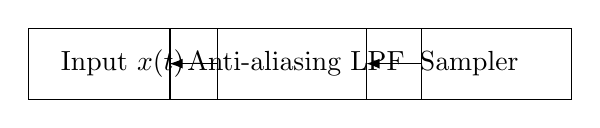
\begin{tikzpicture}[node distance=2.2cm,>=Latex]
\node[draw,minimum width=2.4cm,minimum height=0.9cm] (x) {Input \(x(t)\)};
\node[draw,minimum width=3.2cm,minimum height=0.9cm,right of=x] (lpf) {Anti-aliasing LPF};
\node[draw,minimum width=2.6cm,minimum height=0.9cm,right of=lpf] (sampler) {Sampler};

\draw[->] (x) -- (lpf);
\draw[->] (lpf) -- (sampler);
\end{tikzpicture}
\end{center}

The filter removes frequency components above \(B\).

%%%%%%%%%%%%%%%%%%%%%%%%%%%%%%%%%%%%%%%%%%%%%%%%%%%%%%%%%%%%%%%%%%%%%%%%%%%%%%%%

\section{Ideal Reconstruction}

The original signal can be reconstructed using an ideal low-pass filter with
cutoff \(B\).

%%%%%%%%%%%%%%%%%%%%%%%%%%%%%%%%%%%%%%%%%%%%%%%%%%%%%%%%%%%%%%%%%%%%%%%%%%%%%%%%

\subsection{Interpolation Formula}

\[
\boxed{
x(t)=
\sum_{n=-\infty}^{\infty}
x[n]
\operatorname{sinc}
\left(
\frac{t-nT_s}{T_s}
\right)
}
\]

where

\[
\operatorname{sinc}(x)=
\frac{\sin(\pi x)}{\pi x}.
\]

%%%%%%%%%%%%%%%%%%%%%%%%%%%%%%%%%%%%%%%%%%%%%%%%%%%%%%%%%%%%%%%%%%%%%%%%%%%%%%%%

\section{Interpretation of Sinc Interpolation}

Each sample generates a sinc pulse.

\begin{itemize}
\item The pulse equals 1 at its own sampling instant.
\item It equals 0 at all other sampling instants.
\item Adding all sinc pulses reconstructs the original signal.
\end{itemize}

%%%%%%%%%%%%%%%%%%%%%%%%%%%%%%%%%%%%%%%%%%%%%%%%%%%%%%%%%%%%%%%%%%%%%%%%%%%%%%%%

\section{Under-Sampling}

If

\[
f_s<2B,
\]

the signal is under-sampled.

Example:

\[
B=5\text{ kHz},
\qquad
f_s=8\text{ kHz}.
\]

Since

\[
8<10,
\]

the signal cannot be reconstructed exactly.

%%%%%%%%%%%%%%%%%%%%%%%%%%%%%%%%%%%%%%%%%%%%%%%%%%%%%%%%%%%%%%%%%%%%%%%%%%%%%%%%

\section{Critical Sampling}

When

\[
f_s=2B,
\]

the spectral replicas just touch each other.

This is called \textbf{critical sampling}.

In practice, we usually choose

\[
f_s>2B
\]

to allow a transition band for the anti-aliasing filter.

%%%%%%%%%%%%%%%%%%%%%%%%%%%%%%%%%%%%%%%%%%%%%%%%%%%%%%%%%%%%%%%%%%%%%%%%%%%%%%%%

\section{Over-Sampling}

When

\[
f_s\gg2B,
\]

the system is over-sampled.

Advantages:

\begin{itemize}
\item easier analog filter design,
\item improved noise performance,
\item higher dynamic range.
\end{itemize}

%%%%%%%%%%%%%%%%%%%%%%%%%%%%%%%%%%%%%%%%%%%%%%%%%%%%%%%%%%%%%%%%%%%%%%%%%%%%%%%%

\section{Solved Example 13.1}

A signal is bandlimited to

\[
B=3\text{ kHz}.
\]

Find the minimum sampling frequency.

%%%%%%%%%%%%%%%%%%%%%%%%%%%%%%%%%%%%%%%%%%%%%%%%%%%%%%%%%%%%%%%%%%%%%%%%%%%%%%%%

\subsection{Solution}

\[
f_s^{\min}=2B=6\text{ kHz}.
\]

\[
\boxed{
f_s^{\min}=6\text{ kHz}
}
\]

%%%%%%%%%%%%%%%%%%%%%%%%%%%%%%%%%%%%%%%%%%%%%%%%%%%%%%%%%%%%%%%%%%%%%%%%%%%%%%%%

\section{Solved Example 13.2}

A 7 kHz signal is sampled at

\[
f_s=10\text{ kHz}.
\]

Find the aliased frequency.

%%%%%%%%%%%%%%%%%%%%%%%%%%%%%%%%%%%%%%%%%%%%%%%%%%%%%%%%%%%%%%%%%%%%%%%%%%%%%%%%

\subsection{Solution}

\[
f_a=|7-10|=3\text{ kHz}.
\]

\[
\boxed{
f_a=3\text{ kHz}
}
\]

%%%%%%%%%%%%%%%%%%%%%%%%%%%%%%%%%%%%%%%%%%%%%%%%%%%%%%%%%%%%%%%%%%%%%%%%%%%%%%%%

\section{Solved Example 13.3}

A signal contains frequencies up to

\[
15\text{ kHz}.
\]

Choose a practical sampling frequency.

%%%%%%%%%%%%%%%%%%%%%%%%%%%%%%%%%%%%%%%%%%%%%%%%%%%%%%%%%%%%%%%%%%%%%%%%%%%%%%%%

\subsection{Solution}

Nyquist rate:

\[
2B=30\text{ kHz}.
\]

Choose a slightly higher value:

\[
\boxed{
f_s=36\text{ kHz}
}
\]

(or 40 kHz in practice).

%%%%%%%%%%%%%%%%%%%%%%%%%%%%%%%%%%%%%%%%%%%%%%%%%%%%%%%%%%%%%%%%%%%%%%%%%%%%%%%%

\section{Solved Example 13.4}

Find the discrete-time frequency corresponding to

\[
f=1\text{ kHz},
\qquad
f_s=8\text{ kHz}.
\]

%%%%%%%%%%%%%%%%%%%%%%%%%%%%%%%%%%%%%%%%%%%%%%%%%%%%%%%%%%%%%%%%%%%%%%%%%%%%%%%%

\subsection{Solution}

\[
\omega=
2\pi\frac{f}{f_s}
=
2\pi\frac{1000}{8000}
=
\frac{\pi}{4}.
\]

\[
\boxed{
\omega=\frac{\pi}{4}\text{ rad/sample}
}
\]

%%%%%%%%%%%%%%%%%%%%%%%%%%%%%%%%%%%%%%%%%%%%%%%%%%%%%%%%%%%%%%%%%%%%%%%%%%%%%%%%

\section{Quick Check}

\begin{enumerate}
\item \(T_s=\boxed{1/f_s}\).
\item Nyquist rate \(=\boxed{2B}\).
\item Nyquist frequency \(=\boxed{f_s/2}\).
\item Aliasing occurs when \(\boxed{f_s<2B}\).
\item Reconstruction uses \(\boxed{\text{sinc interpolation}}\).
\end{enumerate}

%%%%%%%%%%%%%%%%%%%%%%%%%%%%%%%%%%%%%%%%%%%%%%%%%%%%%%%%%%%%%%%%%%%%%%%%%%%%%%%%

\begin{tcolorbox}[title=One-Minute Revision,colback=blue!5]

\[
x[n]=x(nT_s)
\]

\[
f_s=\frac{1}{T_s}
\]

\[
x_s(t)=
\sum x(nT_s)\delta(t-nT_s)
\]

\[
X_s(f)=
f_s\sum X(f-kf_s)
\]

Nyquist theorem:

\[
f_s\ge2B
\]

Nyquist frequency:

\[
f_N=\frac{f_s}{2}
\]

Aliasing:

\[
f_a=|f-kf_s|
\]

Reconstruction:

\[
x(t)=
\sum x[n]\,
\operatorname{sinc}
\left(
\frac{t-nT_s}{T_s}
\right)
\]

\end{tcolorbox}
%%%%%%%%%%%%%%%%%%%%%%%%%%%%%%%%%%%%%%%%%%%%%%%%%%%%%%%%%%%%%%%%%%%%%%%%%%%%%%%%
%%%%%%%%%%%%%%%%%%%%%%%%%%%%%%%%%%%%%%%%%%%%%%%%%%%%%%%%%%%%%%%%%%%%%%%%%%%%%%%%
\section{Discrete-Time Processing of Continuous-Time Signals}

A practical DSP system consists of three stages:

\begin{center}
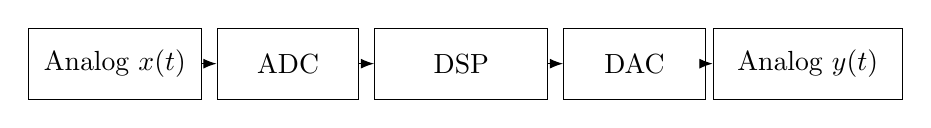
\begin{tikzpicture}[node distance=2.2cm,>=Latex]
\node[draw,minimum width=2.2cm,minimum height=0.9cm] (x) {Analog \(x(t)\)};
\node[draw,minimum width=1.8cm,minimum height=0.9cm,right of=x] (adc) {ADC};
\node[draw,minimum width=2.2cm,minimum height=0.9cm,right of=adc] (dsp) {DSP};
\node[draw,minimum width=1.8cm,minimum height=0.9cm,right of=dsp] (dac) {DAC};
\node[draw,minimum width=2.4cm,minimum height=0.9cm,right of=dac] (y) {Analog \(y(t)\)};

\draw[->] (x) -- (adc);
\draw[->] (adc) -- (dsp);
\draw[->] (dsp) -- (dac);
\draw[->] (dac) -- (y);
\end{tikzpicture}
\end{center}

\begin{itemize}
\item \textbf{ADC}: sampling and quantization.
\item \textbf{DSP}: digital filtering, modulation, FFT, etc.
\item \textbf{DAC}: converts the processed sequence back to analog form.
\end{itemize}

%%%%%%%%%%%%%%%%%%%%%%%%%%%%%%%%%%%%%%%%%%%%%%%%%%%%%%%%%%%%%%%%%%%%%%%%%%%%%%%%

\section{Analog-to-Digital Conversion (ADC)}

The ADC performs two operations:

%%%%%%%%%%%%%%%%%%%%%%%%%%%%%%%%%%%%%%%%%%%%%%%%%%%%%%%%%%%%%%%%%%%%%%%%%%%%%%%%

\subsection{Sampling}

\[
x[n]=x(nT_s)
\]

%%%%%%%%%%%%%%%%%%%%%%%%%%%%%%%%%%%%%%%%%%%%%%%%%%%%%%%%%%%%%%%%%%%%%%%%%%%%%%%%

\subsection{Quantization}

Each sample is rounded to one of a finite number of amplitude levels.

%%%%%%%%%%%%%%%%%%%%%%%%%%%%%%%%%%%%%%%%%%%%%%%%%%%%%%%%%%%%%%%%%%%%%%%%%%%%%%%%

\section{Quantization Levels}

For an \(N_b\)-bit ADC,

\[
\boxed{
L=2^{N_b}
}
\]

levels are available.

%%%%%%%%%%%%%%%%%%%%%%%%%%%%%%%%%%%%%%%%%%%%%%%%%%%%%%%%%%%%%%%%%%%%%%%%%%%%%%%%

\subsection{Examples}

\begin{table}[H]
\centering
\caption{ADC resolution}
\begin{tabular}{|c|c|}
\hline
\textbf{Bits} & \textbf{Levels}\\
\hline
8 & 256\\
10 & 1024\\
12 & 4096\\
16 & 65536\\
\hline
\end{tabular}
\end{table}

%%%%%%%%%%%%%%%%%%%%%%%%%%%%%%%%%%%%%%%%%%%%%%%%%%%%%%%%%%%%%%%%%%%%%%%%%%%%%%%%

\section{Quantization Step Size}

If the input range is

\[
[-V_{\max},\,V_{\max}],
\]

the step size is

\[
\boxed{
\Delta=
\frac{2V_{\max}}{2^{N_b}}
}
\]

%%%%%%%%%%%%%%%%%%%%%%%%%%%%%%%%%%%%%%%%%%%%%%%%%%%%%%%%%%%%%%%%%%%%%%%%%%%%%%%%

\section{Quantization Error}

The error is

\[
e_q=x-x_q.
\]

For an ideal uniform quantizer,

\[
\boxed{
-\frac{\Delta}{2}\le e_q\le\frac{\Delta}{2}
}
\]

and the mean-square error is

\[
\boxed{
P_q=\frac{\Delta^2}{12}.
}
\]

%%%%%%%%%%%%%%%%%%%%%%%%%%%%%%%%%%%%%%%%%%%%%%%%%%%%%%%%%%%%%%%%%%%%%%%%%%%%%%%%

\section{Signal-to-Quantization-Noise Ratio}

For a full-scale sinusoid,

\[
\boxed{
\text{SQNR}_{\text{dB}}
\approx
6.02N_b+1.76
}
\]

%%%%%%%%%%%%%%%%%%%%%%%%%%%%%%%%%%%%%%%%%%%%%%%%%%%%%%%%%%%%%%%%%%%%%%%%%%%%%%%%

\subsection{Example}

For a 12-bit ADC,

\[
\text{SQNR}\approx
6.02(12)+1.76
=
74\text{ dB}.
\]

%%%%%%%%%%%%%%%%%%%%%%%%%%%%%%%%%%%%%%%%%%%%%%%%%%%%%%%%%%%%%%%%%%%%%%%%%%%%%%%%

\section{Digital-to-Analog Conversion (DAC)}

The DAC produces a staircase waveform.

An analog low-pass filter then smooths the staircase to reconstruct the continuous
signal.

%%%%%%%%%%%%%%%%%%%%%%%%%%%%%%%%%%%%%%%%%%%%%%%%%%%%%%%%%%%%%%%%%%%%%%%%%%%%%%%%

\section{Zero-Order Hold (ZOH)}

A practical DAC holds each sample value constant for one sampling period.

The ZOH output is

\[
x_{\text{ZOH}}(t)=x[n],
\qquad nT_s\le t<(n+1)T_s.
\]

%%%%%%%%%%%%%%%%%%%%%%%%%%%%%%%%%%%%%%%%%%%%%%%%%%%%%%%%%%%%%%%%%%%%%%%%%%%%%%%%

\section{ZOH Frequency Response}

The ZOH introduces a sinc-shaped attenuation:

\[
\boxed{
H_{\text{ZOH}}(f)=
T_s\,\mathrm{sinc}(fT_s)\,
e^{-j\pi fT_s}
}
\]

High frequencies are attenuated more than low frequencies.

%%%%%%%%%%%%%%%%%%%%%%%%%%%%%%%%%%%%%%%%%%%%%%%%%%%%%%%%%%%%%%%%%%%%%%%%%%%%%%%%

\section{Sampling of a Sinusoid}

Let

\[
x(t)=A\cos(2\pi f_0 t+\phi).
\]

Sampling at \(f_s\) gives

\[
x[n]=A\cos\left(2\pi\frac{f_0}{f_s}n+\phi\right).
\]

Define the discrete-time frequency

\[
\boxed{
\omega_0=
2\pi\frac{f_0}{f_s}
}
\]

in rad/sample.

%%%%%%%%%%%%%%%%%%%%%%%%%%%%%%%%%%%%%%%%%%%%%%%%%%%%%%%%%%%%%%%%%%%%%%%%%%%%%%%%

\section{Example 1}

\[
f_0=1\text{ kHz},
\qquad
f_s=8\text{ kHz}.
\]

Then

\[
\omega_0=
2\pi\frac{1}{8}
=
\frac{\pi}{4}.
\]

Hence,

\[
\boxed{
x[n]=A\cos\left(\frac{\pi}{4}n+\phi\right)
}
\]

%%%%%%%%%%%%%%%%%%%%%%%%%%%%%%%%%%%%%%%%%%%%%%%%%%%%%%%%%%%%%%%%%%%%%%%%%%%%%%%%

\section{Frequency Equivalence}

Discrete-time frequencies separated by multiples of \(2\pi\) are identical:

\[
\boxed{
\omega\equiv\omega+2\pi k
}
\]

Therefore,

\[
\cos(\omega n)=\cos((\omega+2\pi)n).
\]

%%%%%%%%%%%%%%%%%%%%%%%%%%%%%%%%%%%%%%%%%%%%%%%%%%%%%%%%%%%%%%%%%%%%%%%%%%%%%%%%

\section{Example 2}

\[
\omega_1=\frac{\pi}{4},
\qquad
\omega_2=\frac{9\pi}{4}.
\]

Since

\[
\omega_2=\omega_1+2\pi,
\]

both sequences are identical.

%%%%%%%%%%%%%%%%%%%%%%%%%%%%%%%%%%%%%%%%%%%%%%%%%%%%%%%%%%%%%%%%%%%%%%%%%%%%%%%%

\section{Analog Frequency Mapping}

The analog frequency corresponding to a discrete-time frequency \(\omega\) is

\[
\boxed{
f=\frac{\omega}{2\pi}f_s
}
\]

%%%%%%%%%%%%%%%%%%%%%%%%%%%%%%%%%%%%%%%%%%%%%%%%%%%%%%%%%%%%%%%%%%%%%%%%%%%%%%%%

\subsection{Example}

\[
\omega=\frac{\pi}{2},
\qquad
f_s=10\text{ kHz}.
\]

Then

\[
f=
\frac{\pi/2}{2\pi}(10\,000)
=
2500\text{ Hz}.
\]

\[
\boxed{
f=2.5\text{ kHz}
}
\]

%%%%%%%%%%%%%%%%%%%%%%%%%%%%%%%%%%%%%%%%%%%%%%%%%%%%%%%%%%%%%%%%%%%%%%%%%%%%%%%%

\section{Discrete-Time Filtering of Analog Signals}

Suppose the analog input is sampled to obtain \(x[n]\).

A digital filter with frequency response \(H(e^{j\omega})\) produces

\[
y[n]=x[n]*h[n].
\]

After DAC and reconstruction, the analog output approximates the response of an
analog filter.

%%%%%%%%%%%%%%%%%%%%%%%%%%%%%%%%%%%%%%%%%%%%%%%%%%%%%%%%%%%%%%%%%%%%%%%%%%%%%%%%

\section{Equivalent Analog Frequency}

The digital filter acts on frequencies

\[
0\le\omega\le\pi.
\]

These correspond to analog frequencies

\[
0\le f\le\frac{f_s}{2}.
\]

Thus, digital filter specifications are often converted between \(\omega\) and
\(f\).

%%%%%%%%%%%%%%%%%%%%%%%%%%%%%%%%%%%%%%%%%%%%%%%%%%%%%%%%%%%%%%%%%%%%%%%%%%%%%%%%

\section{Multirate Signal Processing}

%%%%%%%%%%%%%%%%%%%%%%%%%%%%%%%%%%%%%%%%%%%%%%%%%%%%%%%%%%%%%%%%%%%%%%%%%%%%%%%%

\subsection{Decimation}

Reducing the sampling rate by \(M\):

\[
\boxed{
y[n]=x[nM]
}
\]

The new sampling frequency is

\[
f_s'=\frac{f_s}{M}.
\]

An anti-aliasing filter must be applied before decimation.

%%%%%%%%%%%%%%%%%%%%%%%%%%%%%%%%%%%%%%%%%%%%%%%%%%%%%%%%%%%%%%%%%%%%%%%%%%%%%%%%

\section{Interpolation}

Increasing the sampling rate by \(L\):

\begin{enumerate}
\item Insert \(L-1\) zeros between samples.
\item Apply a low-pass interpolation filter.
\end{enumerate}

The new sampling frequency is

\[
f_s'=Lf_s.
\]

%%%%%%%%%%%%%%%%%%%%%%%%%%%%%%%%%%%%%%%%%%%%%%%%%%%%%%%%%%%%%%%%%%%%%%%%%%%%%%%%

\section{Example 3: Decimation}

A signal sampled at

\[
48\text{ kHz}
\]

is decimated by

\[
M=4.
\]

Then

\[
f_s'=
\frac{48}{4}
=
12\text{ kHz}.
\]

\[
\boxed{
f_s'=12\text{ kHz}
}
\]

%%%%%%%%%%%%%%%%%%%%%%%%%%%%%%%%%%%%%%%%%%%%%%%%%%%%%%%%%%%%%%%%%%%%%%%%%%%%%%%%

\section{Example 4: Interpolation}

A signal sampled at

\[
8\text{ kHz}
\]

is interpolated by

\[
L=3.
\]

Then

\[
f_s'=24\text{ kHz}.
\]

\[
\boxed{
f_s'=24\text{ kHz}
}
\]

%%%%%%%%%%%%%%%%%%%%%%%%%%%%%%%%%%%%%%%%%%%%%%%%%%%%%%%%%%%%%%%%%%%%%%%%%%%%%%%%

\section{Bandpass Sampling (Concept)}

A bandpass signal can sometimes be sampled at a rate lower than \(2f_H\), provided
the spectral replicas do not overlap.

This is called \textbf{undersampling} or \textbf{bandpass sampling} and is used in
RF receivers.

For GATE, remember:

\[
\boxed{
2B\le f_s
}
\]

where \(B\) is the bandwidth of the bandpass signal.

%%%%%%%%%%%%%%%%%%%%%%%%%%%%%%%%%%%%%%%%%%%%%%%%%%%%%%%%%%%%%%%%%%%%%%%%%%%%%%%%

\section{Solved Example 13.5}

A signal is bandlimited to

\[
B=5\text{ kHz}.
\]

Find the minimum sampling frequency.

%%%%%%%%%%%%%%%%%%%%%%%%%%%%%%%%%%%%%%%%%%%%%%%%%%%%%%%%%%%%%%%%%%%%%%%%%%%%%%%%

\subsection{Solution}

\[
f_s^{\min}=2B=10\text{ kHz}.
\]

\[
\boxed{
10\text{ kHz}
}
\]

%%%%%%%%%%%%%%%%%%%%%%%%%%%%%%%%%%%%%%%%%%%%%%%%%%%%%%%%%%%%%%%%%%%%%%%%%%%%%%%%

\section{Solved Example 13.6}

A 9 kHz sinusoid is sampled at

\[
f_s=12\text{ kHz}.
\]

Find the aliased frequency.

%%%%%%%%%%%%%%%%%%%%%%%%%%%%%%%%%%%%%%%%%%%%%%%%%%%%%%%%%%%%%%%%%%%%%%%%%%%%%%%%

\subsection{Solution}

Choose \(k=1\):

\[
f_a=|9-12|=3\text{ kHz}.
\]

\[
\boxed{
f_a=3\text{ kHz}
}
\]

%%%%%%%%%%%%%%%%%%%%%%%%%%%%%%%%%%%%%%%%%%%%%%%%%%%%%%%%%%%%%%%%%%%%%%%%%%%%%%%%

\section{Solved Example 13.7}

Find the discrete-time frequency of a 2 kHz signal sampled at 16 kHz.

%%%%%%%%%%%%%%%%%%%%%%%%%%%%%%%%%%%%%%%%%%%%%%%%%%%%%%%%%%%%%%%%%%%%%%%%%%%%%%%%

\subsection{Solution}

\[
\omega=
2\pi\frac{2000}{16000}
=
\frac{\pi}{4}.
\]

\[
\boxed{
\omega=\frac{\pi}{4}\text{ rad/sample}
}
\]

%%%%%%%%%%%%%%%%%%%%%%%%%%%%%%%%%%%%%%%%%%%%%%%%%%%%%%%%%%%%%%%%%%%%%%%%%%%%%%%%

\section{Solved Example 13.8}

A 10-bit ADC has input range

\[
\pm5\text{ V}.
\]

Find the quantization step size.

%%%%%%%%%%%%%%%%%%%%%%%%%%%%%%%%%%%%%%%%%%%%%%%%%%%%%%%%%%%%%%%%%%%%%%%%%%%%%%%%

\subsection{Solution}

\[
\Delta=
\frac{10}{2^{10}}
=
\frac{10}{1024}
=
9.77\text{ mV}.
\]

\[
\boxed{
\Delta\approx9.77\text{ mV}
}
\]

%%%%%%%%%%%%%%%%%%%%%%%%%%%%%%%%%%%%%%%%%%%%%%%%%%%%%%%%%%%%%%%%%%%%%%%%%%%%%%%%

\section{Solved Example 13.9}

Find the SQNR of an 8-bit ADC.

%%%%%%%%%%%%%%%%%%%%%%%%%%%%%%%%%%%%%%%%%%%%%%%%%%%%%%%%%%%%%%%%%%%%%%%%%%%%%%%%

\subsection{Solution}

\[
\text{SQNR}\approx
6.02(8)+1.76
=
49.92\text{ dB}.
\]

\[
\boxed{
\text{SQNR}\approx50\text{ dB}
}
\]

%%%%%%%%%%%%%%%%%%%%%%%%%%%%%%%%%%%%%%%%%%%%%%%%%%%%%%%%%%%%%%%%%%%%%%%%%%%%%%%%

\section{Quick Check}

\begin{enumerate}
\item ADC levels \(=\boxed{2^{N_b}}\).
\item Quantization step \(=\boxed{\dfrac{2V_{\max}}{2^{N_b}}}\).
\item SQNR \(=\boxed{6.02N_b+1.76}\).
\item Discrete-time frequency:
\[
\boxed{\omega=2\pi f/f_s}
\]
\item Decimation:
\[
\boxed{y[n]=x[nM]}
\]
\item Interpolation increases sampling rate by \(\boxed{L}\).
\end{enumerate}

%%%%%%%%%%%%%%%%%%%%%%%%%%%%%%%%%%%%%%%%%%%%%%%%%%%%%%%%%%%%%%%%%%%%%%%%%%%%%%%%

\section{Chapter Summary}

In this chapter, we studied the complete chain of discrete-time processing of
continuous-time signals, including sampling, ADC, quantization, DAC, zero-order
hold, frequency mapping and multirate processing.

We also analyzed aliasing, reconstruction, decimation and interpolation, and
solved several GATE-style numerical problems.

With this chapter, the entire GATE Signals \& Systems syllabus is complete.

%%%%%%%%%%%%%%%%%%%%%%%%%%%%%%%%%%%%%%%%%%%%%%%%%%%%%%%%%%%%%%%%%%%%%%%%%%%%%%%%

\section{Complete Volume Conclusion}

This volume covered

\begin{enumerate}
\item Continuous-time Fourier series,
\item Continuous-time Fourier transform,
\item Sampling theorem,
\item DTFT,
\item DFT,
\item FFT,
\item z-transform,
\item Frequency response,
\item Poles and zeros,
\item Phase delay,
\item Group delay,
\item Discrete-time processing of continuous-time signals.
\end{enumerate}

These topics form the mathematical foundation of

\begin{itemize}
\item Digital Signal Processing,
\item Communication Systems,
\item Control Systems,
\item Embedded DSP,
\item Radar and Sonar,
\item Audio and Speech Processing,
\item Satellite and Aerospace Signal Processing.
\end{itemize}

%%%%%%%%%%%%%%%%%%%%%%%%%%%%%%%%%%%%%%%%%%%%%%%%%%%%%%%%%%%%%%%%%%%%%%%%%%%%%%%%

\begin{tcolorbox}[title=Final One-Minute Revision,colback=blue!5]

Sampling:

\[
x[n]=x(nT_s),
\qquad
f_s=\frac1{T_s}
\]

Nyquist:

\[
f_s\ge2B
\]

Aliasing:

\[
f_a=|f-kf_s|
\]

DTFT:

\[
X(e^{j\omega})=
\sum x[n]e^{-j\omega n}
\]

DFT:

\[
X[k]=
\sum x[n]e^{-j2\pi kn/N}
\]

FFT complexity:

\[
N\log_2N
\]

z-transform:

\[
X(z)=
\sum x[n]z^{-n}
\]

Frequency response:

\[
H(e^{j\omega})=H(z)|_{z=e^{j\omega}}
\]

Group delay:

\[
\tau_g=
-\frac{d\phi}{d\omega}
\]

Linear-phase FIR:

\[
\tau_g=\frac{N-1}{2}
\]

ADC:

\[
L=2^{N_b},
\qquad
\Delta=\frac{2V_{\max}}{2^{N_b}}
\]

SQNR:

\[
6.02N_b+1.76\text{ dB}
\]

\end{tcolorbox}
%%%%%%%%%%%%%%%%%%%%%%%%%%%%%%%%%%%%%%%%%%%%%%%%%%%%%%%%%%%%%%%%%%%%%%%%%%%%%%%%

% =========================================================
% Back Matter
% =========================================================
\backmatter

\chapter*{About This Book}

These notes were prepared for GATE EC preparation with emphasis on conceptual
clarity, derivations, solved examples, and quick revision. The material covers
the complete Signals and Systems syllabus and is intended for both university
examinations and competitive examinations.

\end{document}
